%# -*- coding: utf-8-unix -*-
%%==================================================
%% thesis.tex
%%==================================================


%\newcommand{\argmax}{\mathop{\mathrm{arg\,max}}
%\newcommand{\argmin}{\mathop{\mathrm{argmin}}
%\newcommand{\argmin}{\mathop{\mathrm{arg\,min}\nolimits}
%\newcommand{\argmin}{\mathop{\mathrm{argmin}\nolimits}



\newcommand{\secref}[1]{\ref{#1}节}
\newcommand{\figref}[1]{图\ref{#1}}
\newcommand{\eqnref}[1]{公式\ref{#1}}
\newcommand{\algoref}[1]{算法\ref{#1}}
\newcommand{\tabref}[1]{表\ref{#1}}
\newcommand{\lineref}[1]{第\ref{#1}行}
\newcommand{\bi}[1]{\textbf{\textit{#1}}}


% 双面打印
\documentclass[doctor, openright, twoside, submit]{sjtuthesis}
% \documentclass[bachelor, openany, oneside, submit]{sjtuthesis}
% \documentclass[master, review]{sjtuthesis}
% \documentclass[%
%   bachelor|master|doctor, % 必选项
%   fontset=fandol|windows|mac|ubuntu|adobe|founder, % 字体选项
%   oneside|twoside,        % 单面打印,双面打印(奇偶页交换页边距,默认)
%   openany|openright,      % 可以在奇数或者偶数页开新章|只在奇数页开新章(默认)
%   english,                % 启用英文模版
%   review,     % 盲审论文,隐去作者姓名、学号、导师姓名、致谢、发表论文和参与的项目
%   submit      % 定稿提交的论文,插入签名扫描版的原创性声明、授权声明 
% ]

\usepackage{amsmath}
\usepackage{bm}
%\usepackage[backend=biber,style=gb7714-2015ay%,gbtype=true%,backref=true%gb,gbt7714_2005_n,
%]{biblatex}%biber,caspervector

%\usepackage[backend=biber,bibstyle=gb7714-2015,%nature,%
%citestyle=gb7714-2015%,backref=true%
%]{biblatex}


% 逐个导入参考文献数据库
\addbibresource{bib/thesis.bib}
% \addbibresource{bib/chap2.bib}

\begin{document}

% 无编号内容:中英文论文封面、授权页
%# -*- coding: utf-8-unix -*-
% !TEX program = xelatex
% !TEX root = ../thesis.tex
% !TEX encoding = UTF-8 Unicode
\title{基于知识库的自然语言理解}
\author{罗康琦}
\advisor{朱其立教授}
% \coadvisor{某某教授}
\defenddate{2019年2月21日}
\school{上海交通大学}
\institute{计算机科学与工程系}
\studentnumber{0120339027}
\major{计算机科学与技术}

\englishtitle{Knowledge Base Empowered 

Natural Language Understanding}
\englishauthor{\textsc{Kangqi Luo}}
\englishadvisor{Prof. \textsc{Kenny Qili Zhu}}
\englishschool{Shanghai Jiao Tong University}
\englishinstitute{\textsc{Depart of Computer Science \& Engineering} \\
  \textsc{Shanghai Jiao Tong University} \\
  \textsc{Shanghai, P.R.China}}
\englishmajor{Computer Science and Technology Major}
\englishdate{Feb. 21st, 2019}


\maketitle

\makeatletter
\ifsjtu@submit\relax
  %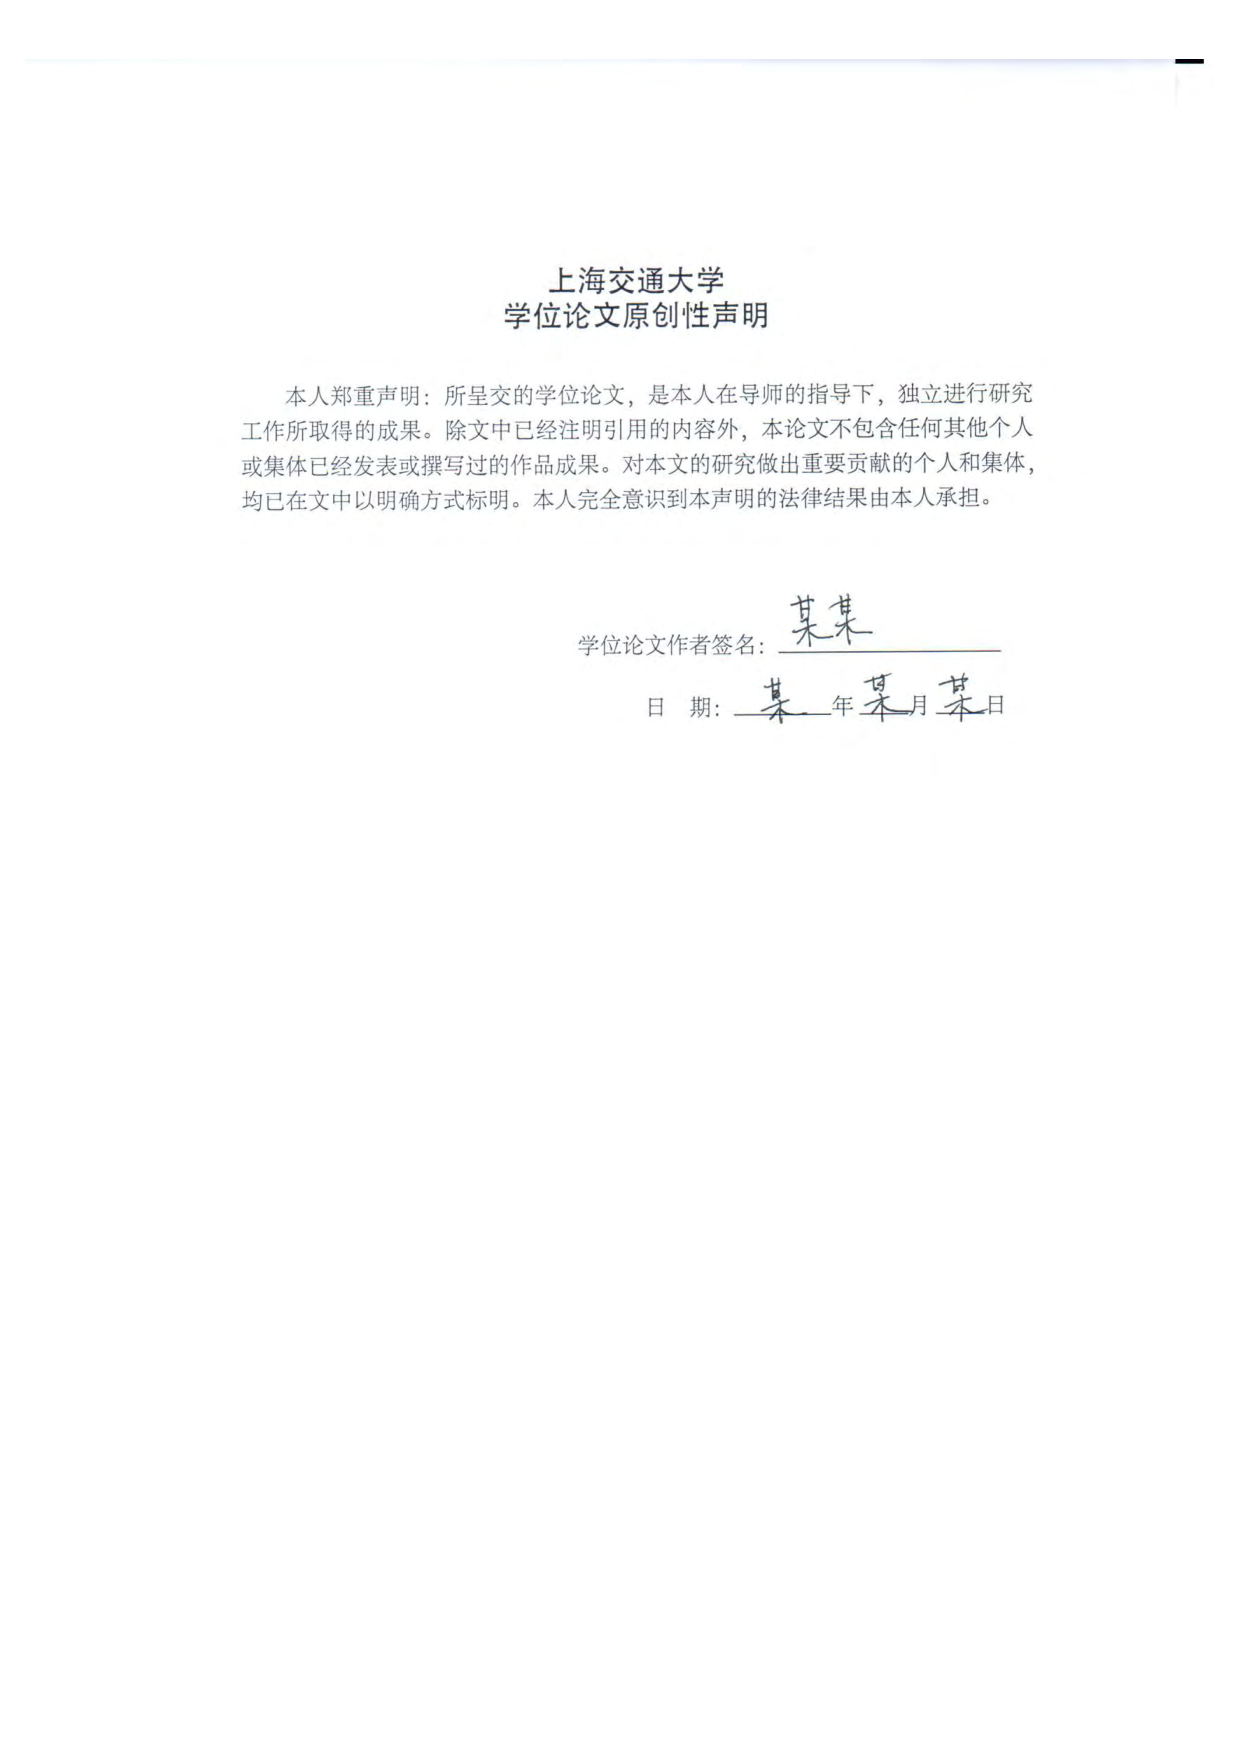
\includepdf{pdf/original.pdf}
  %\cleardoublepage
  %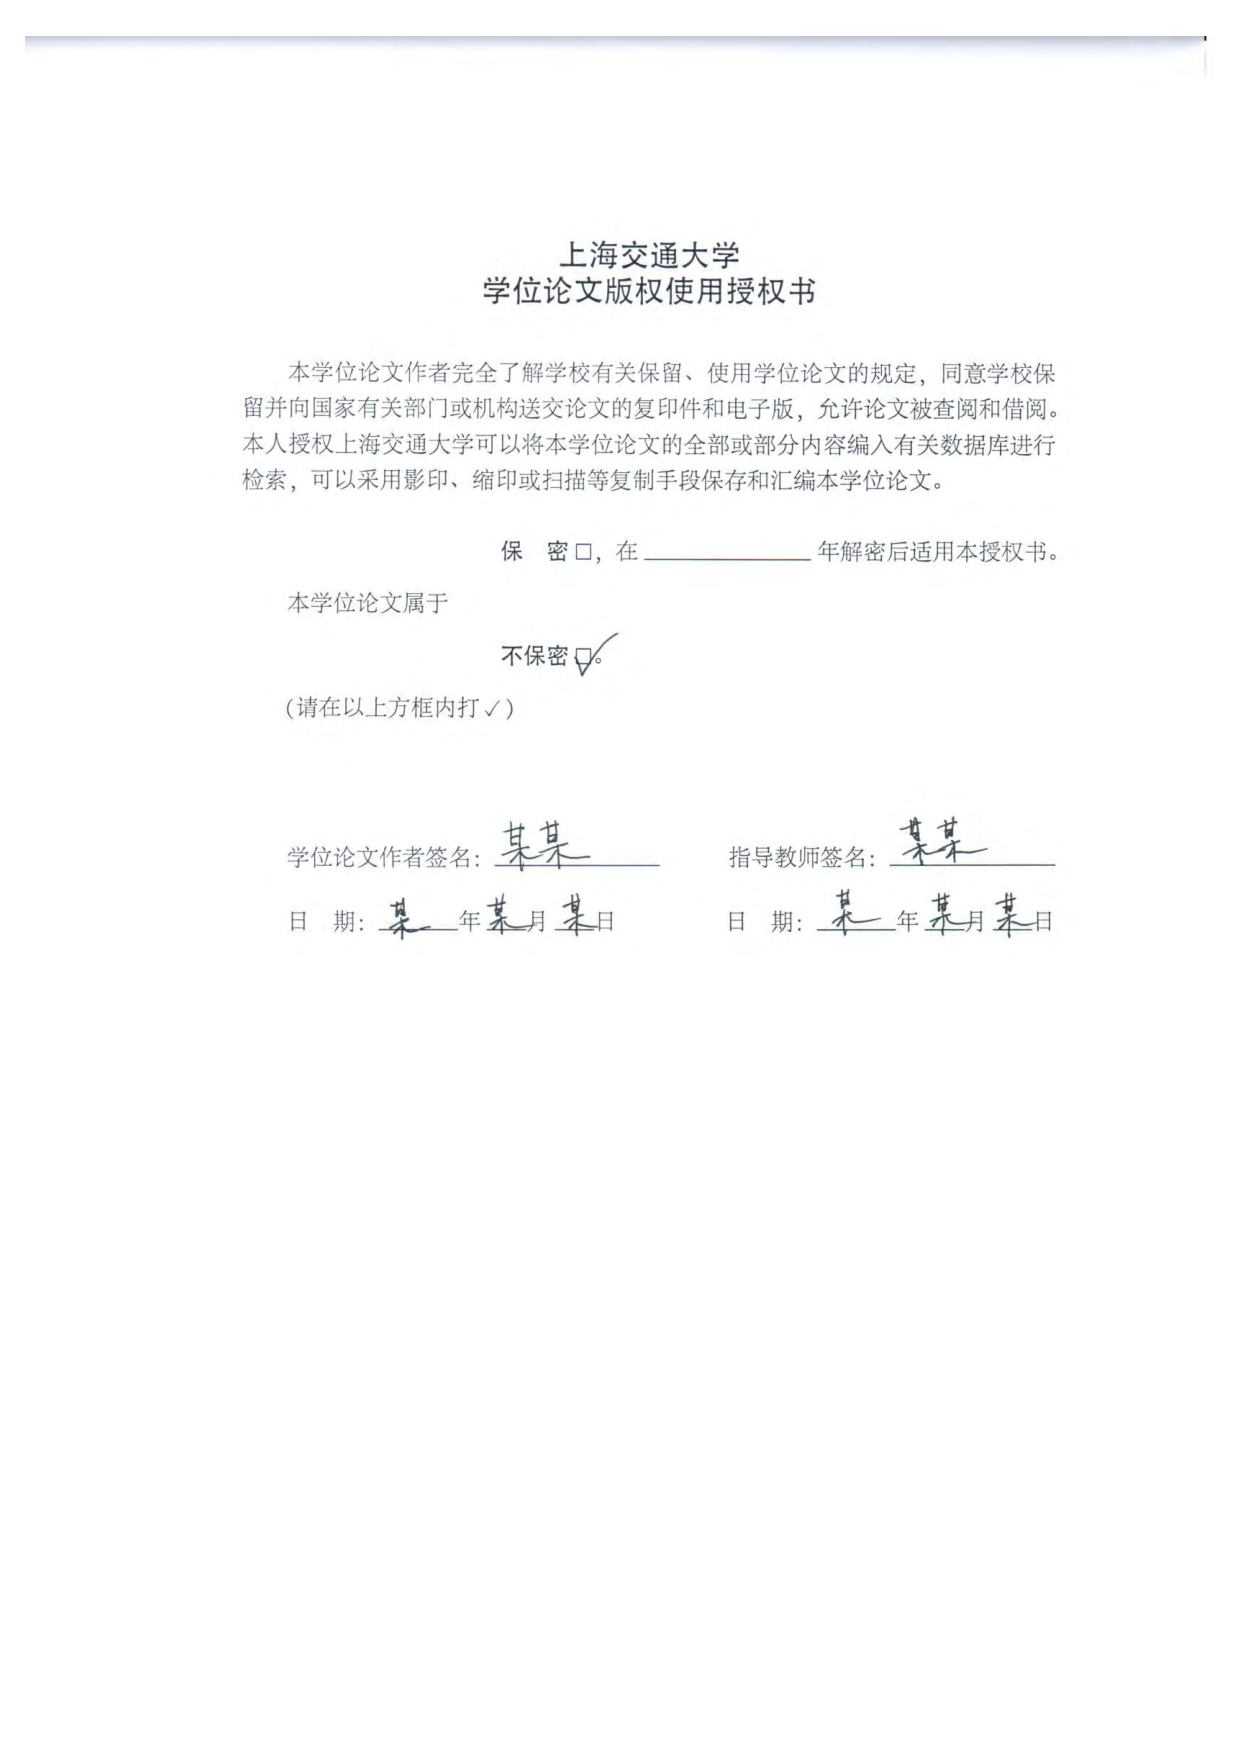
\includepdf{pdf/authorization.pdf}
  %\cleardoublepage
\else
\ifsjtu@review\relax
% exclude the original claim and authorization
\else
  \makeDeclareOriginal
  \makeDeclareAuthorization
\fi
\fi
\makeatother

\frontmatter % 使用罗马数字对前言编号

% 摘要
\begin{abstract}

This paper attempts to discover communication patterns automatically within dog vocalizations
in a data-driven approach, which breaks the barrier previous approaches that rely
on human prior knowledge on limited data. 
We present a self-supervised approach with HuBERT, enabling the accurate classification 
of phones, and an adaptive grammar induction method that identifies phone sequence patterns 
that suggest a preliminary vocabulary within dog vocalizations. 
Our results show that a subset of this vocabulary has substantial causality relations
with certain canine activities, suggesting signs of stable semantics associated with these
``words''.
%We use this approach to undercover phonemes and mine vocabulary of dogs. 
%We further develop a web-based dog vocalization labeling system. This system can highlight phoneme n-grams, present in the vocabulary, in the dog audio uploaded by users.
%This approach can be simply applied to find other non-human language sound units and is valuable for further research on dog language understanding.

\end{abstract}


% 目录、插图目录、表格目录
\tableofcontents
\listoffigures
\addcontentsline{toc}{chapter}{\listfigurename}     % 将插图目录加入全文目录
\listoftables
\addcontentsline{toc}{chapter}{\listtablename}      % 将表格目录加入全文目录
\listofalgorithms
\addcontentsline{toc}{chapter}{\listalgorithmname}  % 将算法目录加入全文目录

%%# -*- coding: utf-8-unix -*-
% !TEX program = xelatex
% !TEX root = ../thesis.tex
% !TEX encoding = UTF-8 Unicode
\begin{nomenclaturename}
\label{chap:symb}

\begin{longtable}{rl}
$\epsilon$     & 介电常数 \\
 $\mu$ 		& 磁导率 \\
 $\epsilon$     & 介电常数 \\
 $\mu$ 		& 磁导率 \\
 $\epsilon$     & 介电常数 \\
 $\mu$ 		& 磁导率 \\
 $\epsilon$ 	& 介电常数 \\
 $\mu$ 		& 磁导率 \\
 $\epsilon$     & 介电常数 \\
 $\mu$ 		& 磁导率 \\
 $\epsilon$     & 介电常数 \\
 $\mu$ 		& 磁导率 \\
 $\epsilon$     & 介电常数 \\
 $\mu$ 		& 磁导率 \\
 $\epsilon$ 	& 介电常数 \\
 $\mu$ 		& 磁导率 \\
 $\epsilon$     & 介电常数 \\
 $\mu$ 		& 磁导率 \\
 $\epsilon$     & 介电常数 \\
 $\mu$ 		& 磁导率 \\
 $\epsilon$     & 介电常数 \\
 $\mu$ 		& 磁导率 \\
 $\epsilon$ 	& 介电常数 \\
 $\mu$ 		& 磁导率 \\
 $\epsilon$     & 介电常数 \\
 $\mu$ 		& 磁导率 \\
 $\epsilon$     & 介电常数 \\
 $\mu$ 		& 磁导率 \\
 $\epsilon$     & 介电常数 \\
 $\mu$ 		& 磁导率 \\
 $\epsilon$ 	& 介电常数 \\
 $\mu$ 		& 磁导率 \\
 $\epsilon$     & 介电常数 \\
 $\mu$ 		& 磁导率 \\
 $\epsilon$     & 介电常数 \\
 $\mu$ 		& 磁导率 \\
 $\epsilon$     & 介电常数 \\
 $\mu$ 		& 磁导率 \\
 $\epsilon$ 	& 介电常数 \\
 $\mu$ 		& 磁导率 \\
 $\epsilon$     & 介电常数 \\
 $\mu$ 		& 磁导率 \\
 $\epsilon$     & 介电常数 \\
 $\mu$ 		& 磁导率 \\
 $\epsilon$     & 介电常数 \\
 $\mu$ 		& 磁导率 \\
 $\epsilon$ 	& 介电常数 \\
 $\mu$ 		& 磁导率 \\
 $\epsilon$     & 介电常数 \\
 $\mu$ 		& 磁导率 \\
 $\epsilon$     & 介电常数 \\
 $\mu$ 		& 磁导率 \\
 $\epsilon$     & 介电常数 \\
 $\mu$ 		& 磁导率 \\
\end{longtable}

\end{nomenclaturename}
 % 主要符号、缩略词对照表

\mainmatter % 使用阿拉伯数字对正文编号

% 正文内容
%\IEEEraisesectionheading{
% %\IEEEraisesectionheading{
% %\IEEEraisesectionheading{
% \input{intro}
\section{Introduction}\label{sec:intro}
 %}
% \section{Introduction}\label{sec:intro}

% \begin{enumerate}
% \item Motivation: application scenarios (with 1-2 running examples);
% \item Characteristics of the data sources and their challenges;
% \item Briefly introduce previous approaches to extract information 
% from images including setting the document zone, and their limitations.
% \item General flow of our approach (may give a diagram here)
% \end{enumerate}
% scenary

Due to ever evolving hardware and software, many medical images
such as electro-cardio graphs (ECGs), X-ray or ultrasound images  
are directly printed and stored in hard copy formats. 
% \KZ{Insert 4 example images here.}
%Examples are shown in \figref{fig:medicalImages}. 
% These images often contain a mix of graphics and text, which
% include parameter settings of the hardware, test measurements or simple
% diagnosis. 
These images often contain a mix of graphics and text, which 
include technical settings of the hardware used, test measurements or simple diagnoses.
Recently, there has been a growing demand for digitizing such 
medical information from paper media sources, especially legacy ones, or patients who want to keep track of these documents by themselves digitally. 
Apart from scanning the graphics into a digital format, extracting 
the semi-structured textual information is also an important part of
building electronic medical records for patients. 

%\begin{figure}[!htb]
%\centering
%\subfloat[ECG]{
%\label{fig:medicalimage:ecg}
%\epsfig{file=figure/17_ori.eps, width=0.4\columnwidth}
%}
%% \hfill
%\subfloat[MRI]{
%	\label{fig:medicalimage:mrt}
%	\epsfig{file=figure/MRI.eps, width=0.4\columnwidth}
%}
%\\
%\subfloat[X-RAY]{
%\label{fig:medicalimage:xray}
%\epsfig{file=figure/X-RAY.eps, width=0.4\columnwidth}
%}
%%\hfill
%\subfloat[EEG]{
%\label{fig:medicalimage:eeg}
%\epsfig{file=figure/EEG.eps, width=0.4\columnwidth}
%}
%\caption{Examples of Medical Images}
%\label{fig:medicalImages}
%\end{figure}

Optical character recognition (OCR)  \cite{mori1992historical,smith2007overview} is 
a traditional technique used to turn images of printed text into machine encoded
text. It is well researched and performs well on plain text 
documents such as novels and reports, for a variety of languages. 
%For example, Tesseract, which is one of 
%the most popular open source multilingual recognizers, logs an error 
%rate of 3.72\% for English words and 3.77\% for simplified 
%Chinese characters\cite{smith2009adapting}. 
%Google Books \cite{googlebooks} and Gutenberg \cite{gutenberg} are
%projects which have scanned a large number of paper books into text for free and open
%access. These projects made exclusive use of OCR for this conversion and 
%achieved high accuracy \cite{vincent2007google} \cite{lebert2008project}. 
% 99\% for Gutenberg project \cite{lebert2008project}. 
% \KZ{Give the accuracy of google and gutenberg if available.}


\begin{figure}[th]
\centering
\epsfig{file=figure/17_b.eps, width=0.8\columnwidth}
\caption{An ECG image with text area (red circle) of interest.}
\label{fig:ecgexample2}
\end{figure}

For a semi-structured medical image, such as 
\figref{fig:ecgexample2}, we would like to extract the attribute-value 
pairs (e.g., {\em Vent. rate = 63 bpm}) and possibly other values such as
date ({\em 18-Nov-2010}) and time ({\em 9:13:02}) since those values endow us with lots of information about the patient. 
Existing OCR software cannot extract such structured information in a straightforward 
fashion, 
but instead it produces rather convoluted results from the whole image, 
similar to those in \figref{fig:ocrre}, which was produced by Tesseract, 
a popular multi-lingual recognizers. 
% \KZ{Maybe include the x-y coordinate info in the output as well?}  

\begin{figure}[th]
\centering
\scriptsize
\begin{verbatim}
<p class="ocr_par" title="box 263 33 444 119">
   <span class="ocr_l" title="box 264 33 336 45">
       <span class="ocrx_w" title="box 264 33 299 45">Vcnt.</span> 
       <span class="ocrx_w" title="box 308 34 336 45">rule</span> 
   </span>
   <span class='ocr_l'>
       <span class="ocrx_w" title="box 264 51 283 64">PR</span> 
       <span class="ocrx_w" title="box 291 51 346 64">Interval</span> 
       <span class="ocrx_w" title="box 389 52 411 64">140</span> 
       <span class="ocrx_w" title="box 420 55 439 64">ms</span> 
   </span>
   ...
   </span>
</p>
<p class="ocr_p" dir="ltr">
   <span class="ocr_l">
       <span class="ocrx_w" title="box 396 33 411 45">53</span> 
       <span class="ocrx_w" title="box 420 33 449 48">bpm</span> 
   </span>
</p>
\end{verbatim}
\caption{Snippet OCR results in XML, input to our framework.}
\label{fig:ocrre}
\end{figure}


%\input{xmlre1}

%However, OCR alone does not work well on semi-structured text and hence
%can't be directly used for information extraction from the aforementioned
%medical images. \KZ{Give the reason here, perhaps because OCR models are
%largely Markov based? So semi-structured data breaks the flow of text.}
%When a medical image is input to an ordinary OCR software, the spatial 
%information of the text components is often lost or mixed with noises
%and errors.
%%The reason is OCR converts the whole images into text data, in which 
%%useful information often mix with noises and errors. 
%In this paper, we would like to extract the attribute-value pairs
%and possibly other values from \figref{fig:ecgexample1} 
%and \figref{fig:ecgexample2}. 
%% or medical ultrasonography report. 
%Such images contain lots of non-textual information or noises.

% example & ref
%\begin{figure}[ht]
%\centering
%\epsfig{file=figure/46.eps, width=0.8\columnwidth}
%\caption{ECG Images From Printer1}
%\label{fig:ecgexample1}
%\end{figure}

% \begin{figure}[ht]
% \centering
% \subfloat[Printer1]{
% \label{fig:ecgexample:a}
% \epsfig{file=figure/46.eps, width=0.48\columnwidth}
% }
% \hfill
% \subfloat[Printer2]{
% \label{fig:ecgexample:b}
% \epsfig{file=figure/17.eps, width=0.48\columnwidth}
% }
% \caption{ECG images from two different printers}
% \label{fig:ecgexample}
% \end{figure}

Also, errors in the OCR text \cite{darwish2007error,taghva1996evaluation} will greatly affect the effectiveness 
of other related tasks. Much work has been done to improve the performance of the OCR\cite{kolak2003generative,cesarini1998informys}. However, there are still a number of significant challenges involved in extracting the information from medical images or OCR results in XML form. 

% First, medical images differ from pure text document in that them have 
% layout information. 
First, medical images differ from pure text documents in that 
they contain layout information.
Although most current OCR engines attempt to reproduce the physical 
layout of the text units, 
%(along with X-Y coordinates) and store them 
%in a special format such as XML 
% (\KZ{Better in the previous example})
such spatial
information is approximate and sometimes inaccurate, which is why neighboring
text blocks in \figref{fig:ecgexample2}, such as ``Vent. Rate'' and
``63 bpm'' were not automatically combined into the same XML block, but were 
rather far apart (shown in two different ``classes'') in \figref{fig:ocrre} made by OCR softwares. 
%Even for images produced by the same ECG printer, 
%the XML results can still be very different as 
The spatial layout is sensitive to many factors, such as accidental spots 
on the prints, color and contrast, or the angle of the camera. 
%In this case, solutions for other application domains, for example, the web, 
%are not well suited for information extraction from printed documents \cite{bartoli2014semisupervised}. With such inaccurate
%layout information produced by OCR,
%it is not easy to write a simple wrapper program to extract useful
%data from images, even if the images come from the same printer. 

%Writing a wrapper for each
%individual image would be tedious and counter-productive. Therefore,
%a mechanism that makes use of the spatial locality of the 
%text units in the image and 
%accommodates slight variations in the spatial layout would make the extraction
%more accurate and fault-tolerant.

%For example, \figref{fig:ocrre} is the simplified OCR results for the ECGs in 
%\figref{fig:ecgexample1} and \figref{fig:ecgexample2}. The results are in the XML format and have attritube named {\em class} 
%for layout information. Although these two images share similar format. 
%OCR engine generates different results in that it splits elements that 
%should be in the same line into two lines in the second example. 
%XML is sensitive to the layout results so it's hard to tolerate 
%all the layout results. 
%
% example check the term
% layout of ocr results can be restore, so why OCR engine don't restore the results 
% using the similar methods as we do?
% or the way we handle the layout problem is quite simple

% Delete for TIP
% Second, exiting OCR engines make heavy use of Markov properties such as n-grams
% since they primarily target the transformation of large body of text 
% \cite{kolak2003generative}. 
% % \KZ{Needs some refs here.}
% Unfortunately, the semi-structured texts in medical images are often 
% short and not even written in complete sentences, thus breaking Markov assumption. To make
% matters worse, medical images contain scientific language, which may be
% very different from the training corpora of these OCR engines.
% This explains why we see errors like ``Vcnt'' and ``rule'' 
% in \figref{fig:ocrre}. 
% %can't guarantee a perfect performance, which means 
% %there are errors and noises in the OCR results.
% %Many of them due to the fact that the data are no longer long, continous
% %sentences, thus breaking the Markov assumption made by many OCR algorithms. 
% %In \figref{fig:ocrresub:b}, ``Vent." is misrecognized as ``Vcnt.". 
% Without sufficient contextual information, OCR may also misrecognize a 
% digit as an alphabetic character, or as another similar digit. 
% Furthermore, the mix of text with images and formatting
% lines often confuses the OCR engine, which is more biased toward full
% text images.
% Exact pattern matching, as used in
% traditional information extraction, doesn't work with such noisy OCR output
% as it doesn't tolerate noises or errors in text. 
% %It's hard to autocorrect these errors 
% %because image quality is the most important affecting factor. 
% %The text we are processing can be full of no meaning words or 
% %strange numbers. 
% A fuzzy matching strategy is more desirable in this case. 
% % example, what are the traditional IEs

Second, there are many types of medical images, resulting from a variety of
medical tests. Different equipments for the same test can produce vastly 
different images. Writing individual extraction wrappers 
for the OCR outputs of all these formats is tedious and inefficient, 
and difficult for non-programmers.
%not to mention that there are significant programming barriers for 
%writing these wrappers, especially for the medical professionals who are the
%end users of these extraction results. 
%A more user-friendly approach enabling users to specify such extraction requirements would be preferred. 
%There are various kinds of medical images, such as electrocardiograph report, 
%medical ultrasonography report, etc. 
%However the basic measures for each type of medical test (e.g., ECG), 
%are very similar from machine to machine. Only the layouts are 
%different. 
% example medical images

Finally, most off-the-shelf OCR programs are pre-trained with specific 
recognition models, which may not be suitable for the extraction of 
%medical images.
%Furthermore, changes in imaging equipment technology over time may produce 
%different formats, layout, or terminology, rendering existing OCR models 
%obsolete. 
Re-training the models requires a large amount of labeled data, which may
not be available. 
%Incremental training as more labeled data arrives
%is currently not supported by any OCR product.    

%There have been some limited attempts to address some of the above challenges. 
%One solution is a plugin of an OCR program that allows the user to specify 
%target zones of interest in the image to be extracted. The zones specified for
%one image can be applied to images with slight variations by adjusting against
%a fixed reference point that is supposed to exist in all these images.
%% \KZ{I think the problem is not so much with the zones, because we also
%% have zones, but rather with the reference point.}
%% \JY{}
%% example products
%% http://www.square-9.com/automated-data-extraction-optical-character-recognition
%The problem with this solution is its high reliance on the OCR zones  
%established by the user. The performance of the results is affected by the 
%accuracy of the zones. If the zones are too big, the results will be full of 
%noise. If the zones are too small, results will miss something. 
%
%Another solution involves using the page layout analysis technique. The page layout 
%analysis technique is used to determine where the text 
%resides on a page \cite{o1993document}, 
%% \KZ{This page layout analysis approach is not clearly described. I don't understand after reading this paragraph.}
%% By using page layout analysis technique, the hierarchy of physical components 
%% can be generated and to match with the hierarchy of logical components, which 
%% is predefined. 
%this includes identifying and categorizing the 
%regions of interest in the scanned image of a text document. 
%Typically, the first step is to segment text zones from 
%non-textual zones and arrange them in their original order. 
%Then in order to analyze the logical roles of the text zones 
%(titles, captions, footnotes, etc.), logical layout analysis 
%is used for labeling the semantics of the text zones.
%Generally, page layout analysis is used for documents. The problem with applying 
%such a technique on medical images is that it creates so much noises 
%that performance is ultimately affected. 
%For medical imaging reports like ECG, useful information is often 
%found in the small components of the image, while most of the images are 
%read as noises. 
% check paper and more description, weakness, ref

%In this paper, 
%we propose a spatial data description language, which borrows its syntax from
%PADS \cite{fisher+:pads}, an ad hoc data processing language, 
%for describing semi-structured data in medical images. 
%% ref
%We call this language OCR description language, or ODL. 
%ODL is designed for extracting and parsing semi-structured text data 
%from images. We believe that  information extraction from those data in ODL form may be much easier than extracting information from rough data or data in XML form, which means that our preprocessing part proves to be necessary.
%%An example ODL description for the image in 
%%\figref{fig:ecgexample2} is shown in 
%%\figref{fig:description}. \KZ{Make this description two column, and give
%%some brief explanation of this description here.} 
%%The parsing result of this description is shown
%%in \figref{fig:parsing result}. \KZ{Give some explanation of the results,
%%otherwise don't show the result here. E.g., you need to explain what F, E, etc.
%%mean. You want to say that even though rate has been recognized as rule,
%%the bpm value was still extracted (but still wrong!).}
%% \KZ{I removed the preprocessing part, cos it's not important. Talk about it in
%% discussion sec.}
%%The our approach starts by preprocessing the images for text results.
%To use this framework, the user first describes the components in the image
%that he or she is interested in extracting. This includes constant strings
%and variables of different data types.   
%ODL allows the user to specify the approximate spatial layout and constraints on
%the data, e.g., integers within 
%a certain range, real numbers with certain decimal points, etc. 
%%This information is then as the key component in our fuzzy matching strategy. 
%The system then automatically generates a parser for these medical images.
%This parser uses the output XML from OCR with spatial information as an input, 
%and outputs a data structure with values extracted for each variables
%in the description, unless there is an unrecoverable error during the parsing process.
%In addition, approximate layout information and constraints are used in parsing process 
%to tolerate noises and small format variations in the input images. 
%%Specifically, this method could be called fuzzy matching, meaning that more candidates could be saved after the parsing process.  It's obvious that we may have a higher probability to obtain the accurate result if more candidates are kept so that fuzzy match should be used properly in our system.
%%An autogenerated parser based on the ODL description can release us from 
%%repetitive work. In this way, we turn the task of writing complex parsers 
%%into describing information on images.
%
%
%When users process many images of the same format, the system 
%automatically discovers parsing errors given the current model and 
%prompts the user to manually correct some of the frequent and prominent
%errors, which effectively serves as an online labeling function. 
%These incrementally labeled data are then used to update the parsing model. 


%It should be emphasized that the incremental learning model is very important in our whole system. Incremental learning is a machine learning paradigm where the learning process takes place whenever we have new examples or data added to our baisc data set, leading to a most striking difference between incremental learning and traditional machine learning: it does not assume the availability of a sufficient training set before the learning process. What incremental learning in our system is really impressive: it does not require a relatively good and stable training set at first time. In fact, it could improve the parsing result with even relatively rough training sets at first by absorbing new data or corrective information as time passes in dynamic systems. Besides, the process would be very effective when there are some new images coming in since training process would not learn from scratch, which might waste time and computation resource.

%At last, we propose an incrementally human correction framwork which can 
%make the best use of human correction to handle the misrecognition problem. 
% Base on our experiments on about 500 real life ECG images, 
% our approach achieves p1 and p2 after p3 times human correction. 
% experimental results

% \begin{figure}[h]
% \begin{lstlisting}
% Oenum str_month_t{
% 	"Jan", "Feb", "Mar", "Apr",
% 	"May", "Jun", "Jul", "Aug",
% 	"Sept", "Oct", "Nov", "Dec"
% };

% Ounion month_t{
% 	Oint(1,12)	num;
% 	str_month_t	str;
% };

% Ostruct time_t{
% 	Oint(1,31)	day;
% 	"-";
% 	month_t	month;
% 	"-";
% 	Oint	year;
% };

% Ostruct triple_t{
% 	"Vent.";
% 	hskip(\s)	skip1;
% 	"rate";
% 	Oint x;
% 	"bpm";
% 	vskip(\n)	skip2;
% };

% Oscource Ostruct entry_t{
% 	time_t(<-,-,-,0.3l>) t;
% 	triple_t(<0.1w,-,0.5w,->) d;
% };
% \end{lstlisting}
% \caption{Description}\label{fig:description}
% \end{figure}


In order to solve above problems, We design a system which makes three main contributions:
\begin{enumerate}
\item Based on some previous work on data description language \cite{lamport1986document,taft1999post,fisher+:pads},we design a new declarative spatial data description language called \textit{OCR description language}, or ODL,
which allows users to specify spatial and data constraints in medical 
images(\secref{sec:syntax});
\item We propose a noise-tolerant parser which takes OCR results
the ODL description as input and outputs a data structure with values 
extracted for each variables in the description (\secref{sec:semantics});
\item We propose an incremental manual correction 
framework\cite{von2008recaptcha,zhu2012learnpads++}, which 
takes advantage of user corrections  and improves the productivity
significantly (\secref{sec:correction}).
%To be more specific, the framework improves the traditional machine learning methods by using a incremental learning process to avoid starting from scratch when we are trying to apply human corrections in the system. That means the framework would be more effective than most corrective systems.
\end{enumerate}


\section{Introduction}\label{sec:intro}
 %}
% \section{Introduction}\label{sec:intro}

% \begin{enumerate}
% \item Motivation: application scenarios (with 1-2 running examples);
% \item Characteristics of the data sources and their challenges;
% \item Briefly introduce previous approaches to extract information 
% from images including setting the document zone, and their limitations.
% \item General flow of our approach (may give a diagram here)
% \end{enumerate}
% scenary

Due to ever evolving hardware and software, many medical images
such as electro-cardio graphs (ECGs), X-ray or ultrasound images  
are directly printed and stored in hard copy formats. 
% \KZ{Insert 4 example images here.}
%Examples are shown in \figref{fig:medicalImages}. 
% These images often contain a mix of graphics and text, which
% include parameter settings of the hardware, test measurements or simple
% diagnosis. 
These images often contain a mix of graphics and text, which 
include technical settings of the hardware used, test measurements or simple diagnoses.
Recently, there has been a growing demand for digitizing such 
medical information from paper media sources, especially legacy ones, or patients who want to keep track of these documents by themselves digitally. 
Apart from scanning the graphics into a digital format, extracting 
the semi-structured textual information is also an important part of
building electronic medical records for patients. 

%\begin{figure}[!htb]
%\centering
%\subfloat[ECG]{
%\label{fig:medicalimage:ecg}
%\epsfig{file=figure/17_ori.eps, width=0.4\columnwidth}
%}
%% \hfill
%\subfloat[MRI]{
%	\label{fig:medicalimage:mrt}
%	\epsfig{file=figure/MRI.eps, width=0.4\columnwidth}
%}
%\\
%\subfloat[X-RAY]{
%\label{fig:medicalimage:xray}
%\epsfig{file=figure/X-RAY.eps, width=0.4\columnwidth}
%}
%%\hfill
%\subfloat[EEG]{
%\label{fig:medicalimage:eeg}
%\epsfig{file=figure/EEG.eps, width=0.4\columnwidth}
%}
%\caption{Examples of Medical Images}
%\label{fig:medicalImages}
%\end{figure}

Optical character recognition (OCR)  \cite{mori1992historical,smith2007overview} is 
a traditional technique used to turn images of printed text into machine encoded
text. It is well researched and performs well on plain text 
documents such as novels and reports, for a variety of languages. 
%For example, Tesseract, which is one of 
%the most popular open source multilingual recognizers, logs an error 
%rate of 3.72\% for English words and 3.77\% for simplified 
%Chinese characters\cite{smith2009adapting}. 
%Google Books \cite{googlebooks} and Gutenberg \cite{gutenberg} are
%projects which have scanned a large number of paper books into text for free and open
%access. These projects made exclusive use of OCR for this conversion and 
%achieved high accuracy \cite{vincent2007google} \cite{lebert2008project}. 
% 99\% for Gutenberg project \cite{lebert2008project}. 
% \KZ{Give the accuracy of google and gutenberg if available.}


\begin{figure}[th]
\centering
\epsfig{file=figure/17_b.eps, width=0.8\columnwidth}
\caption{An ECG image with text area (red circle) of interest.}
\label{fig:ecgexample2}
\end{figure}

For a semi-structured medical image, such as 
\figref{fig:ecgexample2}, we would like to extract the attribute-value 
pairs (e.g., {\em Vent. rate = 63 bpm}) and possibly other values such as
date ({\em 18-Nov-2010}) and time ({\em 9:13:02}) since those values endow us with lots of information about the patient. 
Existing OCR software cannot extract such structured information in a straightforward 
fashion, 
but instead it produces rather convoluted results from the whole image, 
similar to those in \figref{fig:ocrre}, which was produced by Tesseract, 
a popular multi-lingual recognizers. 
% \KZ{Maybe include the x-y coordinate info in the output as well?}  

\begin{figure}[th]
\centering
\scriptsize
\begin{verbatim}
<p class="ocr_par" title="box 263 33 444 119">
   <span class="ocr_l" title="box 264 33 336 45">
       <span class="ocrx_w" title="box 264 33 299 45">Vcnt.</span> 
       <span class="ocrx_w" title="box 308 34 336 45">rule</span> 
   </span>
   <span class='ocr_l'>
       <span class="ocrx_w" title="box 264 51 283 64">PR</span> 
       <span class="ocrx_w" title="box 291 51 346 64">Interval</span> 
       <span class="ocrx_w" title="box 389 52 411 64">140</span> 
       <span class="ocrx_w" title="box 420 55 439 64">ms</span> 
   </span>
   ...
   </span>
</p>
<p class="ocr_p" dir="ltr">
   <span class="ocr_l">
       <span class="ocrx_w" title="box 396 33 411 45">53</span> 
       <span class="ocrx_w" title="box 420 33 449 48">bpm</span> 
   </span>
</p>
\end{verbatim}
\caption{Snippet OCR results in XML, input to our framework.}
\label{fig:ocrre}
\end{figure}


%% \begin{figure}[ht]
% \centering
% \subfigure[]{
% \label{fig:subfig:a}
% \begin{minipage}[b]{0.2\textwidth}
%\newsavebox{\firstlisting}
%\begin{lrbox}{\firstlisting}% Store first listing
%\begin{lstlisting}
%<p class='ocr_par' dir='ltr'>
%   <span class='ocr_line' id='line_2'>
%       <span class='ocrx_word' id='word_6'>Vent.</span>
%       <span class='ocrx_word' id='word_7'>rate</span>
%       <span class='ocrx_word' id='word_8'>65</span>
%       <span class='ocrx_word' id='word_9'>bpm</span>
%   </span>
%   <span class='ocr_line' id='line_3'>
%       <span class='ocrx_word' id='word_14'>PR</span>
%       <span class='ocrx_word' id='word_15'>interval</span>
%       <span class='ocrx_word' id='word_16'>162</span>
%       <span class='ocrx_word' id='word_17'>ms</span>
%   </span>
%    ...
%</p>
%\end{lstlisting}
%\end{lrbox}
% \end{minipage}
% }
% \hspace[1in]
% \subfigure[]{
% % \label{fig:subfig:b}
% % \begin{minipage}[b]{0.2\textwidth}
\newsavebox{\secondlisting}
\begin{lrbox}{\secondlisting}
% \tiny
\begin{lstlisting}[basicstyle=\tiny,]
<p class="ocr_par" title="box 263 33 444 119">
   <span class="ocr_l" title="box 264 33 336 45">
       <span class="ocrx_w" title="box 264 33 299 45">Vcnt.</span>
       <span class="ocrx_w" title="box 308 34 336 45">rule</span>
   </span>
   <span class='ocr_l'>
       <span class="ocrx_w" title="box 264 51 283 64">PR</span>
       <span class="ocrx_w" title="box 291 51 346 64">Interval</span>
       <span class="ocrx_w" title="box 389 52 411 64">140</span>
       <span class="ocrx_w" title="box 420 55 439 64">ms</span>
   </span>
   ...
   </span>
</p>
<p class="ocr_p" dir="ltr">
   <span class="ocr_l">
       <span class="ocrx_w" title="box 396 33 411 45">53</span>
       <span class="ocrx_w" title="box 420 33 449 48">bpm</span>
   </span>
</p>
\end{lstlisting}
\end{lrbox}
% % \end{minipage}
% }

% \KZ{\figref{fig:ocrre} is output from what software? Tesseract?}
\begin{figure*}[th]
%\subfloat[Image From Printer1]{
%\label{fig:ocrresub:a}
%\scalebox{0.8}{\usebox{\firstlisting}}}
%\hfill
%\subfloat[Image From Printer2]{
\scalebox{1.6}{\usebox{\secondlisting}}
% \label{fig:ocrre}
\caption{A fragment of raw OCR results for ECG with layout information.}
%\caption{Simplified OCR Results in XML for an ECG with Layout Information}
%\label{fig:ocrresub:b}
\label{fig:running-xml}
\end{figure*}

% \lipsum[2]


%However, OCR alone does not work well on semi-structured text and hence
%can't be directly used for information extraction from the aforementioned
%medical images. \KZ{Give the reason here, perhaps because OCR models are
%largely Markov based? So semi-structured data breaks the flow of text.}
%When a medical image is input to an ordinary OCR software, the spatial 
%information of the text components is often lost or mixed with noises
%and errors.
%%The reason is OCR converts the whole images into text data, in which 
%%useful information often mix with noises and errors. 
%In this paper, we would like to extract the attribute-value pairs
%and possibly other values from \figref{fig:ecgexample1} 
%and \figref{fig:ecgexample2}. 
%% or medical ultrasonography report. 
%Such images contain lots of non-textual information or noises.

% example & ref
%\begin{figure}[ht]
%\centering
%\epsfig{file=figure/46.eps, width=0.8\columnwidth}
%\caption{ECG Images From Printer1}
%\label{fig:ecgexample1}
%\end{figure}

% \begin{figure}[ht]
% \centering
% \subfloat[Printer1]{
% \label{fig:ecgexample:a}
% \epsfig{file=figure/46.eps, width=0.48\columnwidth}
% }
% \hfill
% \subfloat[Printer2]{
% \label{fig:ecgexample:b}
% \epsfig{file=figure/17.eps, width=0.48\columnwidth}
% }
% \caption{ECG images from two different printers}
% \label{fig:ecgexample}
% \end{figure}

Also, errors in the OCR text \cite{darwish2007error,taghva1996evaluation} will greatly affect the effectiveness 
of other related tasks. Much work has been done to improve the performance of the OCR\cite{kolak2003generative,cesarini1998informys}. However, there are still a number of significant challenges involved in extracting the information from medical images or OCR results in XML form. 

% First, medical images differ from pure text document in that them have 
% layout information. 
First, medical images differ from pure text documents in that 
they contain layout information.
Although most current OCR engines attempt to reproduce the physical 
layout of the text units, 
%(along with X-Y coordinates) and store them 
%in a special format such as XML 
% (\KZ{Better in the previous example})
such spatial
information is approximate and sometimes inaccurate, which is why neighboring
text blocks in \figref{fig:ecgexample2}, such as ``Vent. Rate'' and
``63 bpm'' were not automatically combined into the same XML block, but were 
rather far apart (shown in two different ``classes'') in \figref{fig:ocrre} made by OCR softwares. 
%Even for images produced by the same ECG printer, 
%the XML results can still be very different as 
The spatial layout is sensitive to many factors, such as accidental spots 
on the prints, color and contrast, or the angle of the camera. 
%In this case, solutions for other application domains, for example, the web, 
%are not well suited for information extraction from printed documents \cite{bartoli2014semisupervised}. With such inaccurate
%layout information produced by OCR,
%it is not easy to write a simple wrapper program to extract useful
%data from images, even if the images come from the same printer. 

%Writing a wrapper for each
%individual image would be tedious and counter-productive. Therefore,
%a mechanism that makes use of the spatial locality of the 
%text units in the image and 
%accommodates slight variations in the spatial layout would make the extraction
%more accurate and fault-tolerant.

%For example, \figref{fig:ocrre} is the simplified OCR results for the ECGs in 
%\figref{fig:ecgexample1} and \figref{fig:ecgexample2}. The results are in the XML format and have attritube named {\em class} 
%for layout information. Although these two images share similar format. 
%OCR engine generates different results in that it splits elements that 
%should be in the same line into two lines in the second example. 
%XML is sensitive to the layout results so it's hard to tolerate 
%all the layout results. 
%
% example check the term
% layout of ocr results can be restore, so why OCR engine don't restore the results 
% using the similar methods as we do?
% or the way we handle the layout problem is quite simple

% Delete for TIP
% Second, exiting OCR engines make heavy use of Markov properties such as n-grams
% since they primarily target the transformation of large body of text 
% \cite{kolak2003generative}. 
% % \KZ{Needs some refs here.}
% Unfortunately, the semi-structured texts in medical images are often 
% short and not even written in complete sentences, thus breaking Markov assumption. To make
% matters worse, medical images contain scientific language, which may be
% very different from the training corpora of these OCR engines.
% This explains why we see errors like ``Vcnt'' and ``rule'' 
% in \figref{fig:ocrre}. 
% %can't guarantee a perfect performance, which means 
% %there are errors and noises in the OCR results.
% %Many of them due to the fact that the data are no longer long, continous
% %sentences, thus breaking the Markov assumption made by many OCR algorithms. 
% %In \figref{fig:ocrresub:b}, ``Vent." is misrecognized as ``Vcnt.". 
% Without sufficient contextual information, OCR may also misrecognize a 
% digit as an alphabetic character, or as another similar digit. 
% Furthermore, the mix of text with images and formatting
% lines often confuses the OCR engine, which is more biased toward full
% text images.
% Exact pattern matching, as used in
% traditional information extraction, doesn't work with such noisy OCR output
% as it doesn't tolerate noises or errors in text. 
% %It's hard to autocorrect these errors 
% %because image quality is the most important affecting factor. 
% %The text we are processing can be full of no meaning words or 
% %strange numbers. 
% A fuzzy matching strategy is more desirable in this case. 
% % example, what are the traditional IEs

Second, there are many types of medical images, resulting from a variety of
medical tests. Different equipments for the same test can produce vastly 
different images. Writing individual extraction wrappers 
for the OCR outputs of all these formats is tedious and inefficient, 
and difficult for non-programmers.
%not to mention that there are significant programming barriers for 
%writing these wrappers, especially for the medical professionals who are the
%end users of these extraction results. 
%A more user-friendly approach enabling users to specify such extraction requirements would be preferred. 
%There are various kinds of medical images, such as electrocardiograph report, 
%medical ultrasonography report, etc. 
%However the basic measures for each type of medical test (e.g., ECG), 
%are very similar from machine to machine. Only the layouts are 
%different. 
% example medical images

Finally, most off-the-shelf OCR programs are pre-trained with specific 
recognition models, which may not be suitable for the extraction of 
%medical images.
%Furthermore, changes in imaging equipment technology over time may produce 
%different formats, layout, or terminology, rendering existing OCR models 
%obsolete. 
Re-training the models requires a large amount of labeled data, which may
not be available. 
%Incremental training as more labeled data arrives
%is currently not supported by any OCR product.    

%There have been some limited attempts to address some of the above challenges. 
%One solution is a plugin of an OCR program that allows the user to specify 
%target zones of interest in the image to be extracted. The zones specified for
%one image can be applied to images with slight variations by adjusting against
%a fixed reference point that is supposed to exist in all these images.
%% \KZ{I think the problem is not so much with the zones, because we also
%% have zones, but rather with the reference point.}
%% \JY{}
%% example products
%% http://www.square-9.com/automated-data-extraction-optical-character-recognition
%The problem with this solution is its high reliance on the OCR zones  
%established by the user. The performance of the results is affected by the 
%accuracy of the zones. If the zones are too big, the results will be full of 
%noise. If the zones are too small, results will miss something. 
%
%Another solution involves using the page layout analysis technique. The page layout 
%analysis technique is used to determine where the text 
%resides on a page \cite{o1993document}, 
%% \KZ{This page layout analysis approach is not clearly described. I don't understand after reading this paragraph.}
%% By using page layout analysis technique, the hierarchy of physical components 
%% can be generated and to match with the hierarchy of logical components, which 
%% is predefined. 
%this includes identifying and categorizing the 
%regions of interest in the scanned image of a text document. 
%Typically, the first step is to segment text zones from 
%non-textual zones and arrange them in their original order. 
%Then in order to analyze the logical roles of the text zones 
%(titles, captions, footnotes, etc.), logical layout analysis 
%is used for labeling the semantics of the text zones.
%Generally, page layout analysis is used for documents. The problem with applying 
%such a technique on medical images is that it creates so much noises 
%that performance is ultimately affected. 
%For medical imaging reports like ECG, useful information is often 
%found in the small components of the image, while most of the images are 
%read as noises. 
% check paper and more description, weakness, ref

%In this paper, 
%we propose a spatial data description language, which borrows its syntax from
%PADS \cite{fisher+:pads}, an ad hoc data processing language, 
%for describing semi-structured data in medical images. 
%% ref
%We call this language OCR description language, or ODL. 
%ODL is designed for extracting and parsing semi-structured text data 
%from images. We believe that  information extraction from those data in ODL form may be much easier than extracting information from rough data or data in XML form, which means that our preprocessing part proves to be necessary.
%%An example ODL description for the image in 
%%\figref{fig:ecgexample2} is shown in 
%%\figref{fig:description}. \KZ{Make this description two column, and give
%%some brief explanation of this description here.} 
%%The parsing result of this description is shown
%%in \figref{fig:parsing result}. \KZ{Give some explanation of the results,
%%otherwise don't show the result here. E.g., you need to explain what F, E, etc.
%%mean. You want to say that even though rate has been recognized as rule,
%%the bpm value was still extracted (but still wrong!).}
%% \KZ{I removed the preprocessing part, cos it's not important. Talk about it in
%% discussion sec.}
%%The our approach starts by preprocessing the images for text results.
%To use this framework, the user first describes the components in the image
%that he or she is interested in extracting. This includes constant strings
%and variables of different data types.   
%ODL allows the user to specify the approximate spatial layout and constraints on
%the data, e.g., integers within 
%a certain range, real numbers with certain decimal points, etc. 
%%This information is then as the key component in our fuzzy matching strategy. 
%The system then automatically generates a parser for these medical images.
%This parser uses the output XML from OCR with spatial information as an input, 
%and outputs a data structure with values extracted for each variables
%in the description, unless there is an unrecoverable error during the parsing process.
%In addition, approximate layout information and constraints are used in parsing process 
%to tolerate noises and small format variations in the input images. 
%%Specifically, this method could be called fuzzy matching, meaning that more candidates could be saved after the parsing process.  It's obvious that we may have a higher probability to obtain the accurate result if more candidates are kept so that fuzzy match should be used properly in our system.
%%An autogenerated parser based on the ODL description can release us from 
%%repetitive work. In this way, we turn the task of writing complex parsers 
%%into describing information on images.
%
%
%When users process many images of the same format, the system 
%automatically discovers parsing errors given the current model and 
%prompts the user to manually correct some of the frequent and prominent
%errors, which effectively serves as an online labeling function. 
%These incrementally labeled data are then used to update the parsing model. 


%It should be emphasized that the incremental learning model is very important in our whole system. Incremental learning is a machine learning paradigm where the learning process takes place whenever we have new examples or data added to our baisc data set, leading to a most striking difference between incremental learning and traditional machine learning: it does not assume the availability of a sufficient training set before the learning process. What incremental learning in our system is really impressive: it does not require a relatively good and stable training set at first time. In fact, it could improve the parsing result with even relatively rough training sets at first by absorbing new data or corrective information as time passes in dynamic systems. Besides, the process would be very effective when there are some new images coming in since training process would not learn from scratch, which might waste time and computation resource.

%At last, we propose an incrementally human correction framwork which can 
%make the best use of human correction to handle the misrecognition problem. 
% Base on our experiments on about 500 real life ECG images, 
% our approach achieves p1 and p2 after p3 times human correction. 
% experimental results

% \begin{figure}[h]
% \begin{lstlisting}
% Oenum str_month_t{
% 	"Jan", "Feb", "Mar", "Apr",
% 	"May", "Jun", "Jul", "Aug",
% 	"Sept", "Oct", "Nov", "Dec"
% };

% Ounion month_t{
% 	Oint(1,12)	num;
% 	str_month_t	str;
% };

% Ostruct time_t{
% 	Oint(1,31)	day;
% 	"-";
% 	month_t	month;
% 	"-";
% 	Oint	year;
% };

% Ostruct triple_t{
% 	"Vent.";
% 	hskip(\s)	skip1;
% 	"rate";
% 	Oint x;
% 	"bpm";
% 	vskip(\n)	skip2;
% };

% Oscource Ostruct entry_t{
% 	time_t(<-,-,-,0.3l>) t;
% 	triple_t(<0.1w,-,0.5w,->) d;
% };
% \end{lstlisting}
% \caption{Description}\label{fig:description}
% \end{figure}


In order to solve above problems, We design a system which makes three main contributions:
\begin{enumerate}
\item Based on some previous work on data description language \cite{lamport1986document,taft1999post,fisher+:pads},we design a new declarative spatial data description language called \textit{OCR description language}, or ODL,
which allows users to specify spatial and data constraints in medical 
images(\secref{sec:syntax});
\item We propose a noise-tolerant parser which takes OCR results
the ODL description as input and outputs a data structure with values 
extracted for each variables in the description (\secref{sec:semantics});
\item We propose an incremental manual correction 
framework\cite{von2008recaptcha,zhu2012learnpads++}, which 
takes advantage of user corrections  and improves the productivity
significantly (\secref{sec:correction}).
%To be more specific, the framework improves the traditional machine learning methods by using a incremental learning process to avoid starting from scratch when we are trying to apply human corrections in the system. That means the framework would be more effective than most corrective systems.
\end{enumerate}


\section{Introduction}\label{sec:intro}
 %}
% \section{Introduction}\label{sec:intro}

% \begin{enumerate}
% \item Motivation: application scenarios (with 1-2 running examples);
% \item Characteristics of the data sources and their challenges;
% \item Briefly introduce previous approaches to extract information 
% from images including setting the document zone, and their limitations.
% \item General flow of our approach (may give a diagram here)
% \end{enumerate}
% scenary

Due to ever evolving hardware and software, many medical images
such as electro-cardio graphs (ECGs), X-ray or ultrasound images  
are directly printed and stored in hard copy formats. 
% \KZ{Insert 4 example images here.}
%Examples are shown in \figref{fig:medicalImages}. 
% These images often contain a mix of graphics and text, which
% include parameter settings of the hardware, test measurements or simple
% diagnosis. 
These images often contain a mix of graphics and text, which 
include technical settings of the hardware used, test measurements or simple diagnoses.
Recently, there has been a growing demand for digitizing such 
medical information from paper media sources, especially legacy ones, or patients who want to keep track of these documents by themselves digitally. 
Apart from scanning the graphics into a digital format, extracting 
the semi-structured textual information is also an important part of
building electronic medical records for patients. 

%\begin{figure}[!htb]
%\centering
%\subfloat[ECG]{
%\label{fig:medicalimage:ecg}
%\epsfig{file=figure/17_ori.eps, width=0.4\columnwidth}
%}
%% \hfill
%\subfloat[MRI]{
%	\label{fig:medicalimage:mrt}
%	\epsfig{file=figure/MRI.eps, width=0.4\columnwidth}
%}
%\\
%\subfloat[X-RAY]{
%\label{fig:medicalimage:xray}
%\epsfig{file=figure/X-RAY.eps, width=0.4\columnwidth}
%}
%%\hfill
%\subfloat[EEG]{
%\label{fig:medicalimage:eeg}
%\epsfig{file=figure/EEG.eps, width=0.4\columnwidth}
%}
%\caption{Examples of Medical Images}
%\label{fig:medicalImages}
%\end{figure}

Optical character recognition (OCR)  \cite{mori1992historical,smith2007overview} is 
a traditional technique used to turn images of printed text into machine encoded
text. It is well researched and performs well on plain text 
documents such as novels and reports, for a variety of languages. 
%For example, Tesseract, which is one of 
%the most popular open source multilingual recognizers, logs an error 
%rate of 3.72\% for English words and 3.77\% for simplified 
%Chinese characters\cite{smith2009adapting}. 
%Google Books \cite{googlebooks} and Gutenberg \cite{gutenberg} are
%projects which have scanned a large number of paper books into text for free and open
%access. These projects made exclusive use of OCR for this conversion and 
%achieved high accuracy \cite{vincent2007google} \cite{lebert2008project}. 
% 99\% for Gutenberg project \cite{lebert2008project}. 
% \KZ{Give the accuracy of google and gutenberg if available.}


\begin{figure}[th]
\centering
\epsfig{file=figure/17_b.eps, width=0.8\columnwidth}
\caption{An ECG image with text area (red circle) of interest.}
\label{fig:ecgexample2}
\end{figure}

For a semi-structured medical image, such as 
\figref{fig:ecgexample2}, we would like to extract the attribute-value 
pairs (e.g., {\em Vent. rate = 63 bpm}) and possibly other values such as
date ({\em 18-Nov-2010}) and time ({\em 9:13:02}) since those values endow us with lots of information about the patient. 
Existing OCR software cannot extract such structured information in a straightforward 
fashion, 
but instead it produces rather convoluted results from the whole image, 
similar to those in \figref{fig:ocrre}, which was produced by Tesseract, 
a popular multi-lingual recognizers. 
% \KZ{Maybe include the x-y coordinate info in the output as well?}  

\begin{figure}[th]
\centering
\scriptsize
\begin{verbatim}
<p class="ocr_par" title="box 263 33 444 119">
   <span class="ocr_l" title="box 264 33 336 45">
       <span class="ocrx_w" title="box 264 33 299 45">Vcnt.</span> 
       <span class="ocrx_w" title="box 308 34 336 45">rule</span> 
   </span>
   <span class='ocr_l'>
       <span class="ocrx_w" title="box 264 51 283 64">PR</span> 
       <span class="ocrx_w" title="box 291 51 346 64">Interval</span> 
       <span class="ocrx_w" title="box 389 52 411 64">140</span> 
       <span class="ocrx_w" title="box 420 55 439 64">ms</span> 
   </span>
   ...
   </span>
</p>
<p class="ocr_p" dir="ltr">
   <span class="ocr_l">
       <span class="ocrx_w" title="box 396 33 411 45">53</span> 
       <span class="ocrx_w" title="box 420 33 449 48">bpm</span> 
   </span>
</p>
\end{verbatim}
\caption{Snippet OCR results in XML, input to our framework.}
\label{fig:ocrre}
\end{figure}


%% \begin{figure}[ht]
% \centering
% \subfigure[]{
% \label{fig:subfig:a}
% \begin{minipage}[b]{0.2\textwidth}
%\newsavebox{\firstlisting}
%\begin{lrbox}{\firstlisting}% Store first listing
%\begin{lstlisting}
%<p class='ocr_par' dir='ltr'>
%   <span class='ocr_line' id='line_2'>
%       <span class='ocrx_word' id='word_6'>Vent.</span>
%       <span class='ocrx_word' id='word_7'>rate</span>
%       <span class='ocrx_word' id='word_8'>65</span>
%       <span class='ocrx_word' id='word_9'>bpm</span>
%   </span>
%   <span class='ocr_line' id='line_3'>
%       <span class='ocrx_word' id='word_14'>PR</span>
%       <span class='ocrx_word' id='word_15'>interval</span>
%       <span class='ocrx_word' id='word_16'>162</span>
%       <span class='ocrx_word' id='word_17'>ms</span>
%   </span>
%    ...
%</p>
%\end{lstlisting}
%\end{lrbox}
% \end{minipage}
% }
% \hspace[1in]
% \subfigure[]{
% % \label{fig:subfig:b}
% % \begin{minipage}[b]{0.2\textwidth}
\newsavebox{\secondlisting}
\begin{lrbox}{\secondlisting}
% \tiny
\begin{lstlisting}[basicstyle=\tiny,]
<p class="ocr_par" title="box 263 33 444 119">
   <span class="ocr_l" title="box 264 33 336 45">
       <span class="ocrx_w" title="box 264 33 299 45">Vcnt.</span>
       <span class="ocrx_w" title="box 308 34 336 45">rule</span>
   </span>
   <span class='ocr_l'>
       <span class="ocrx_w" title="box 264 51 283 64">PR</span>
       <span class="ocrx_w" title="box 291 51 346 64">Interval</span>
       <span class="ocrx_w" title="box 389 52 411 64">140</span>
       <span class="ocrx_w" title="box 420 55 439 64">ms</span>
   </span>
   ...
   </span>
</p>
<p class="ocr_p" dir="ltr">
   <span class="ocr_l">
       <span class="ocrx_w" title="box 396 33 411 45">53</span>
       <span class="ocrx_w" title="box 420 33 449 48">bpm</span>
   </span>
</p>
\end{lstlisting}
\end{lrbox}
% % \end{minipage}
% }

% \KZ{\figref{fig:ocrre} is output from what software? Tesseract?}
\begin{figure*}[th]
%\subfloat[Image From Printer1]{
%\label{fig:ocrresub:a}
%\scalebox{0.8}{\usebox{\firstlisting}}}
%\hfill
%\subfloat[Image From Printer2]{
\scalebox{1.6}{\usebox{\secondlisting}}
% \label{fig:ocrre}
\caption{A fragment of raw OCR results for ECG with layout information.}
%\caption{Simplified OCR Results in XML for an ECG with Layout Information}
%\label{fig:ocrresub:b}
\label{fig:running-xml}
\end{figure*}

% \lipsum[2]


%However, OCR alone does not work well on semi-structured text and hence
%can't be directly used for information extraction from the aforementioned
%medical images. \KZ{Give the reason here, perhaps because OCR models are
%largely Markov based? So semi-structured data breaks the flow of text.}
%When a medical image is input to an ordinary OCR software, the spatial 
%information of the text components is often lost or mixed with noises
%and errors.
%%The reason is OCR converts the whole images into text data, in which 
%%useful information often mix with noises and errors. 
%In this paper, we would like to extract the attribute-value pairs
%and possibly other values from \figref{fig:ecgexample1} 
%and \figref{fig:ecgexample2}. 
%% or medical ultrasonography report. 
%Such images contain lots of non-textual information or noises.

% example & ref
%\begin{figure}[ht]
%\centering
%\epsfig{file=figure/46.eps, width=0.8\columnwidth}
%\caption{ECG Images From Printer1}
%\label{fig:ecgexample1}
%\end{figure}

% \begin{figure}[ht]
% \centering
% \subfloat[Printer1]{
% \label{fig:ecgexample:a}
% \epsfig{file=figure/46.eps, width=0.48\columnwidth}
% }
% \hfill
% \subfloat[Printer2]{
% \label{fig:ecgexample:b}
% \epsfig{file=figure/17.eps, width=0.48\columnwidth}
% }
% \caption{ECG images from two different printers}
% \label{fig:ecgexample}
% \end{figure}

Also, errors in the OCR text \cite{darwish2007error,taghva1996evaluation} will greatly affect the effectiveness 
of other related tasks. Much work has been done to improve the performance of the OCR\cite{kolak2003generative,cesarini1998informys}. However, there are still a number of significant challenges involved in extracting the information from medical images or OCR results in XML form. 

% First, medical images differ from pure text document in that them have 
% layout information. 
First, medical images differ from pure text documents in that 
they contain layout information.
Although most current OCR engines attempt to reproduce the physical 
layout of the text units, 
%(along with X-Y coordinates) and store them 
%in a special format such as XML 
% (\KZ{Better in the previous example})
such spatial
information is approximate and sometimes inaccurate, which is why neighboring
text blocks in \figref{fig:ecgexample2}, such as ``Vent. Rate'' and
``63 bpm'' were not automatically combined into the same XML block, but were 
rather far apart (shown in two different ``classes'') in \figref{fig:ocrre} made by OCR softwares. 
%Even for images produced by the same ECG printer, 
%the XML results can still be very different as 
The spatial layout is sensitive to many factors, such as accidental spots 
on the prints, color and contrast, or the angle of the camera. 
%In this case, solutions for other application domains, for example, the web, 
%are not well suited for information extraction from printed documents \cite{bartoli2014semisupervised}. With such inaccurate
%layout information produced by OCR,
%it is not easy to write a simple wrapper program to extract useful
%data from images, even if the images come from the same printer. 

%Writing a wrapper for each
%individual image would be tedious and counter-productive. Therefore,
%a mechanism that makes use of the spatial locality of the 
%text units in the image and 
%accommodates slight variations in the spatial layout would make the extraction
%more accurate and fault-tolerant.

%For example, \figref{fig:ocrre} is the simplified OCR results for the ECGs in 
%\figref{fig:ecgexample1} and \figref{fig:ecgexample2}. The results are in the XML format and have attritube named {\em class} 
%for layout information. Although these two images share similar format. 
%OCR engine generates different results in that it splits elements that 
%should be in the same line into two lines in the second example. 
%XML is sensitive to the layout results so it's hard to tolerate 
%all the layout results. 
%
% example check the term
% layout of ocr results can be restore, so why OCR engine don't restore the results 
% using the similar methods as we do?
% or the way we handle the layout problem is quite simple

% Delete for TIP
% Second, exiting OCR engines make heavy use of Markov properties such as n-grams
% since they primarily target the transformation of large body of text 
% \cite{kolak2003generative}. 
% % \KZ{Needs some refs here.}
% Unfortunately, the semi-structured texts in medical images are often 
% short and not even written in complete sentences, thus breaking Markov assumption. To make
% matters worse, medical images contain scientific language, which may be
% very different from the training corpora of these OCR engines.
% This explains why we see errors like ``Vcnt'' and ``rule'' 
% in \figref{fig:ocrre}. 
% %can't guarantee a perfect performance, which means 
% %there are errors and noises in the OCR results.
% %Many of them due to the fact that the data are no longer long, continous
% %sentences, thus breaking the Markov assumption made by many OCR algorithms. 
% %In \figref{fig:ocrresub:b}, ``Vent." is misrecognized as ``Vcnt.". 
% Without sufficient contextual information, OCR may also misrecognize a 
% digit as an alphabetic character, or as another similar digit. 
% Furthermore, the mix of text with images and formatting
% lines often confuses the OCR engine, which is more biased toward full
% text images.
% Exact pattern matching, as used in
% traditional information extraction, doesn't work with such noisy OCR output
% as it doesn't tolerate noises or errors in text. 
% %It's hard to autocorrect these errors 
% %because image quality is the most important affecting factor. 
% %The text we are processing can be full of no meaning words or 
% %strange numbers. 
% A fuzzy matching strategy is more desirable in this case. 
% % example, what are the traditional IEs

Second, there are many types of medical images, resulting from a variety of
medical tests. Different equipments for the same test can produce vastly 
different images. Writing individual extraction wrappers 
for the OCR outputs of all these formats is tedious and inefficient, 
and difficult for non-programmers.
%not to mention that there are significant programming barriers for 
%writing these wrappers, especially for the medical professionals who are the
%end users of these extraction results. 
%A more user-friendly approach enabling users to specify such extraction requirements would be preferred. 
%There are various kinds of medical images, such as electrocardiograph report, 
%medical ultrasonography report, etc. 
%However the basic measures for each type of medical test (e.g., ECG), 
%are very similar from machine to machine. Only the layouts are 
%different. 
% example medical images

Finally, most off-the-shelf OCR programs are pre-trained with specific 
recognition models, which may not be suitable for the extraction of 
%medical images.
%Furthermore, changes in imaging equipment technology over time may produce 
%different formats, layout, or terminology, rendering existing OCR models 
%obsolete. 
Re-training the models requires a large amount of labeled data, which may
not be available. 
%Incremental training as more labeled data arrives
%is currently not supported by any OCR product.    

%There have been some limited attempts to address some of the above challenges. 
%One solution is a plugin of an OCR program that allows the user to specify 
%target zones of interest in the image to be extracted. The zones specified for
%one image can be applied to images with slight variations by adjusting against
%a fixed reference point that is supposed to exist in all these images.
%% \KZ{I think the problem is not so much with the zones, because we also
%% have zones, but rather with the reference point.}
%% \JY{}
%% example products
%% http://www.square-9.com/automated-data-extraction-optical-character-recognition
%The problem with this solution is its high reliance on the OCR zones  
%established by the user. The performance of the results is affected by the 
%accuracy of the zones. If the zones are too big, the results will be full of 
%noise. If the zones are too small, results will miss something. 
%
%Another solution involves using the page layout analysis technique. The page layout 
%analysis technique is used to determine where the text 
%resides on a page \cite{o1993document}, 
%% \KZ{This page layout analysis approach is not clearly described. I don't understand after reading this paragraph.}
%% By using page layout analysis technique, the hierarchy of physical components 
%% can be generated and to match with the hierarchy of logical components, which 
%% is predefined. 
%this includes identifying and categorizing the 
%regions of interest in the scanned image of a text document. 
%Typically, the first step is to segment text zones from 
%non-textual zones and arrange them in their original order. 
%Then in order to analyze the logical roles of the text zones 
%(titles, captions, footnotes, etc.), logical layout analysis 
%is used for labeling the semantics of the text zones.
%Generally, page layout analysis is used for documents. The problem with applying 
%such a technique on medical images is that it creates so much noises 
%that performance is ultimately affected. 
%For medical imaging reports like ECG, useful information is often 
%found in the small components of the image, while most of the images are 
%read as noises. 
% check paper and more description, weakness, ref

%In this paper, 
%we propose a spatial data description language, which borrows its syntax from
%PADS \cite{fisher+:pads}, an ad hoc data processing language, 
%for describing semi-structured data in medical images. 
%% ref
%We call this language OCR description language, or ODL. 
%ODL is designed for extracting and parsing semi-structured text data 
%from images. We believe that  information extraction from those data in ODL form may be much easier than extracting information from rough data or data in XML form, which means that our preprocessing part proves to be necessary.
%%An example ODL description for the image in 
%%\figref{fig:ecgexample2} is shown in 
%%\figref{fig:description}. \KZ{Make this description two column, and give
%%some brief explanation of this description here.} 
%%The parsing result of this description is shown
%%in \figref{fig:parsing result}. \KZ{Give some explanation of the results,
%%otherwise don't show the result here. E.g., you need to explain what F, E, etc.
%%mean. You want to say that even though rate has been recognized as rule,
%%the bpm value was still extracted (but still wrong!).}
%% \KZ{I removed the preprocessing part, cos it's not important. Talk about it in
%% discussion sec.}
%%The our approach starts by preprocessing the images for text results.
%To use this framework, the user first describes the components in the image
%that he or she is interested in extracting. This includes constant strings
%and variables of different data types.   
%ODL allows the user to specify the approximate spatial layout and constraints on
%the data, e.g., integers within 
%a certain range, real numbers with certain decimal points, etc. 
%%This information is then as the key component in our fuzzy matching strategy. 
%The system then automatically generates a parser for these medical images.
%This parser uses the output XML from OCR with spatial information as an input, 
%and outputs a data structure with values extracted for each variables
%in the description, unless there is an unrecoverable error during the parsing process.
%In addition, approximate layout information and constraints are used in parsing process 
%to tolerate noises and small format variations in the input images. 
%%Specifically, this method could be called fuzzy matching, meaning that more candidates could be saved after the parsing process.  It's obvious that we may have a higher probability to obtain the accurate result if more candidates are kept so that fuzzy match should be used properly in our system.
%%An autogenerated parser based on the ODL description can release us from 
%%repetitive work. In this way, we turn the task of writing complex parsers 
%%into describing information on images.
%
%
%When users process many images of the same format, the system 
%automatically discovers parsing errors given the current model and 
%prompts the user to manually correct some of the frequent and prominent
%errors, which effectively serves as an online labeling function. 
%These incrementally labeled data are then used to update the parsing model. 


%It should be emphasized that the incremental learning model is very important in our whole system. Incremental learning is a machine learning paradigm where the learning process takes place whenever we have new examples or data added to our baisc data set, leading to a most striking difference between incremental learning and traditional machine learning: it does not assume the availability of a sufficient training set before the learning process. What incremental learning in our system is really impressive: it does not require a relatively good and stable training set at first time. In fact, it could improve the parsing result with even relatively rough training sets at first by absorbing new data or corrective information as time passes in dynamic systems. Besides, the process would be very effective when there are some new images coming in since training process would not learn from scratch, which might waste time and computation resource.

%At last, we propose an incrementally human correction framwork which can 
%make the best use of human correction to handle the misrecognition problem. 
% Base on our experiments on about 500 real life ECG images, 
% our approach achieves p1 and p2 after p3 times human correction. 
% experimental results

% \begin{figure}[h]
% \begin{lstlisting}
% Oenum str_month_t{
% 	"Jan", "Feb", "Mar", "Apr",
% 	"May", "Jun", "Jul", "Aug",
% 	"Sept", "Oct", "Nov", "Dec"
% };

% Ounion month_t{
% 	Oint(1,12)	num;
% 	str_month_t	str;
% };

% Ostruct time_t{
% 	Oint(1,31)	day;
% 	"-";
% 	month_t	month;
% 	"-";
% 	Oint	year;
% };

% Ostruct triple_t{
% 	"Vent.";
% 	hskip(\s)	skip1;
% 	"rate";
% 	Oint x;
% 	"bpm";
% 	vskip(\n)	skip2;
% };

% Oscource Ostruct entry_t{
% 	time_t(<-,-,-,0.3l>) t;
% 	triple_t(<0.1w,-,0.5w,->) d;
% };
% \end{lstlisting}
% \caption{Description}\label{fig:description}
% \end{figure}


In order to solve above problems, We design a system which makes three main contributions:
\begin{enumerate}
\item Based on some previous work on data description language \cite{lamport1986document,taft1999post,fisher+:pads},we design a new declarative spatial data description language called \textit{OCR description language}, or ODL,
which allows users to specify spatial and data constraints in medical 
images(\secref{sec:syntax});
\item We propose a noise-tolerant parser which takes OCR results
the ODL description as input and outputs a data structure with values 
extracted for each variables in the description (\secref{sec:semantics});
\item We propose an incremental manual correction 
framework\cite{von2008recaptcha,zhu2012learnpads++}, which 
takes advantage of user corrections  and improves the productivity
significantly (\secref{sec:correction}).
%To be more specific, the framework improves the traditional machine learning methods by using a incremental learning process to avoid starting from scratch when we are trying to apply human corrections in the system. That means the framework would be more effective than most corrective systems.
\end{enumerate}


%# -*- coding: utf-8-unix -*-
% !TEX program = xelatex
% !TEX root = ../thesis.tex
% !TEX encoding = UTF-8 Unicode

\chapter{国内外相关研究综述}
\label{chap:rw}


本章中,我们将围绕具体任务,介绍实体、关系、问句语义理解的基础知识和研究综述。
实体理解部分,我们从传统的实体链接任务出发,介绍在文本和表格中的特征工程和深度学习模型,
以及用于跨语言实体链接任务中的跨语言词向量模型;
关系理解部分,我们关注知识库补全任务,并介绍两类主要的模型,分别是规则推导模型和知识库向量模型;
问句理解部分,我们将注意力放在面向客观事实类问题的知识库自动问答任务,
同样介绍两类模型,即基于语义解析和基于信息抽取的模型,前者与我们的研究更加密切,
本节也会重点阐述语义解析模型的多个组成部分。

%# -*- coding: utf-8-unix -*-
% !TEX program = xelatex
% !TEX root = ../thesis.tex
% !TEX encoding = UTF-8 Unicode

\section{实体理解:实体链接任务}
\label{sec:rw-linking}


实体链接任务是一类从自然语言文本中识别出代表实体的字符串,
并将其映射到知识库中特定实体的任务。
人工进行的实体链接体现在维基百科的页面编辑过程中,
页面作者会手动为部分代表实体的短语添加超链接,
指向对应实体的维基页面。
这种带有维基内部超链接的短语被称为锚文本(Anchor Text),
本文中也称为实体短语。
基于机器学习的实体链接可以应用于不同场合的文本输入,
背后所使用的目标知识库也不局限于维基百科,
其它常用的知识库包括DBPedia,Yago以及Freebase。
考虑到这些知识库均基于维基百科信息构建而成,
实体链接任务又被称为``{维基化}'' (Wikification)
\cite{mihalcea2007wikify}。

以英文维基百科为例,一个典型的实体链接任务见下例:

\vspace{0.2cm}
%\begin{minipage}{0.5\columnwidth}
%\begin{center}
\underline{Michael Jordan}, also known by his initials, MJ, 
is a former professional \underline{basketball}
player. He played 15 seasons in the 
\underline{National Basketball Association} for 
the \underline{Chicago Bulls}
and \underline{Washington Wizards}.
%\end{center}
%\end{minipage}
\vspace{0.2cm}

实体链接任务首先需要提取出句中存在的实体短语,即下划线对应的部分。
该步骤与命名实体识别任务类似,
不同之处在于我们关注的实体短语除了命名实体
(具体的人名、地名、组织名、书名、电影名等)之外,
还包含了维基百科中存在的概念实体,用于指代一组相似实体。%例如森林、哺乳动物、运动员等。
下一个步骤对每个实体短语从维基百科中抽取出候选实体集,
并定义短语和候选实体之间的匹配分数,从而将短语链接至最相关的候选实体,
例如句中的5个实体短语分别对应维基百科中的实体
\textit{Michael Jordan}\footnote{https://en.wikipedia.org/wiki/Michael\_Jordan},
\textit{basketball}\footnote{https://en.wikipedia.org/wiki/Basketball},
\textit{National Basketball Association}\footnote{https://en.wikipedia.org/wiki/National\_Basketball\_Association},
\textit{Chicago Bulls}\footnote{https://en.wikipedia.org/wiki/Chicago\_Bulls}
以及\textit{Washington Wizards}\footnote{https://en.wikipedia.org/wiki/Washington\_Wizards}。

除了无结构的纯文本以外,互联网语料中的表格也蕴含了大量与实体相关的知识。
对表格进行实体链接的研究起源于Limaye等人\cite{limaye2010annotating}的工作,
如\figref{fig:rw-linking-limaye}所示,除了每个单元格所对应的实体之外,
得益于半结构化的组织形式,同一表列内的实体通常具有相同的类型,
而且两列实体之间描述了同一种关系的不同实例,
这些是非结构化文本所不具备的优势。
因为表格带来了丰富关系知识,表格上的实体链接在近年来受到了更多的关注。

\begin{figure}[th]
	\centering
    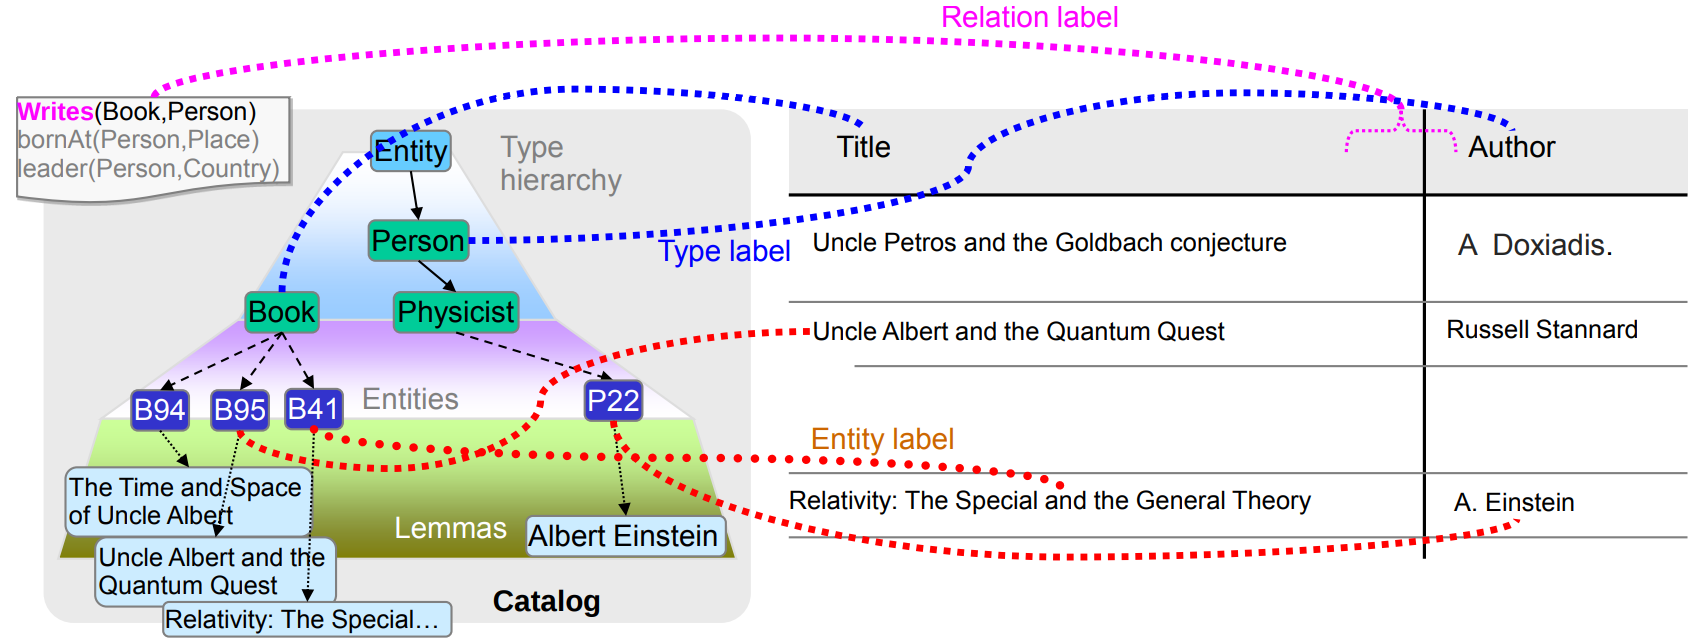
\includegraphics[width=0.95\columnwidth]{figure/rw/linking-limaye.png}
	\bicaption{Limaye等人提出的表格链接任务。\cite{limaye2010annotating}}{Entity linking task on web tables proposed by Limaye et al.}
	\label{fig:rw-linking-limaye}
\end{figure}

%讲一下和下游任务的联系,分别列举,从Han的变来
作为自然语言理解中的基本任务,实体链接是一系列下游任务的前置步骤。
%例如关系分类、阅读理解以及自动问答,
%(加上引用,有了论文就知道怎么聊)
%=============%
首先,开放式信息抽取抽取的主谓宾三元组均为文本表示,通常具有歧义,
一些研究工作旨在对三元组中的实体短语进行链接,
代表文献包括\parencite{nakashole2012patty,lin2012entity},
在实现三元组消歧的同时,结合知识库推理出主语和宾语所代表的类型,
有助于挖掘不同谓词关系之间的语义联系。
%=============%
其次,实体链接与知识库补全任务密切相关,
%带链接的关系三元组与知识库补全任务密切相关,
该任务的目的是向已有知识库中补充新的事实三元组。
这些新添加的三元组主要来源于两方面:
随时间发展所产生的全新事实,或基于已有知识的归纳推理。
基于前者的补全依赖于信息抽取系统的不断挖掘,
因此对主宾语的链接的准确率决定了知识库补全的效果。
知识库补全的相关内容将在\secref{sec:rw-kbc}中论述。
%=============%
最后,对于自动问答任务,%此处加cite?
尤其是我们关注的基于知识库的事实类自动问答任务,
其描述的是与问句中实体相关的事实,
因此不管以何种方式对答案进行建模,都依赖于对已有实体的准确定位,
以限定问句对应语义的搜索范围。
%=============%
%Information Retrieval以及Context Analysis
%都是非常重要的子任务
%实体链接结果给句子提供了知识库维度上的特征,
%并且限定整句的语义范围。
因此,实体链接的结果好坏,对这些任务的效果均有着很大程度的影响。
%常用的数据集包括xxxxx,以及表格数据集xxx

%以下是实体链接任务中的主要数据集。
%TAC-KBP\cite{}是xxxx,包含了xxxx的xxxx。
%AIDA数据集\cite{}由Hoffart等人提出,包含了。。。。
%Web Manual数据集\cite{}
%此外还有相关语料库,例如FACC1\cite{}...
%数据集:(Tutorial71-77)

实体链接的重点在于从多个候选中找出正确的那个实体,
其本质为消除实体级别存在的一词多义性,
例如短语 ``Michael Jordan'' 具有多个可能的候选,
在维基百科中可能代表篮球明星、足球运动员、著名的机器学习教授,
甚至更多不那么有名的人。
在缺乏上下文信息的情况下,很难进行准确的链接。
因此,一个良好的实体链接模型,相关性分数需要考虑多个因素,
包括实体本身的先验知识,实体与短语的匹配程度,以及实体与短语所在上下文的契合度。

基于特征工程的方式,其信息来源主要为维基百科上的统计数据。
随着深度学习的发展,
实体链接的研究将重心放在用表示学习替代或改良传统的特征工程方法。
得益于也文本的向量表示技术,以及神经网络的特征学习能力,
深度学习方法通过计算文本、实体的向量作为其语义表达,
并利用高维空间的相似度衡量短语和候选实体之间的相关性,
在效果上也取得了不错的提升。
接下来的几个小节主要介绍基于特征工程和深度学习的实体链接模型,
并单独介绍用于跨语言链接场景中的跨语言词向量技术。


\subsection{基于特征工程的实体链接}
\label{sec:rw-linking-feature}

基于特征工程的实体链接方法,较为经典的工作包括文献
\parencite{hoffart2011robust,ratinov2011local,shen2012linden,yang2015s,luo2015joint}。
这类方法的共性在于用预定义好的函数或概率值,
描述候选实体与实体短语及其上下文之间的特征,
通过学习特征的带权相加计算最终的匹配度。


在这类方法中,一个候选实体所具有的特征可以分为三类:
先验特征,上下文语义特征,以及与句中其它实体的关联特征。
%=======================%
先验特征与短语所处的文本无关,
仅基于短语与候选实体在维基百科中的统计信息,
主要体现为短语所在锚文本链接至该实体的概率,
以及实体出现在不同维基页面中的概率。
%=======================%
上下文语义特征关注文本及目标实体的语义近似程度,
利用词袋模型(Bag-of-Words)将短语的上下文
以及目标实体的维基页面分别转化为向量形式,
通过TF-IDF得到不同词语的重要性,
并用向量间的相似度
%(余弦相似度,点积或KL散度)
代表语义匹配程度。
%=======================%
实体间的关联特征体现在不同短语所对应的实体之间,
它们维基百科页面的相关性有助于实体链接的判断。
在维基百科中,若两个实体同时指向的页面较多,
或同时指向这两个实体页面的其它实体较多,
则它们具有较高的相关度。
常用的计算方式主要为点对点互信息(PMI)\cite{ratinov2011local}
或基于谷歌距离的维基链接度量(WLM)\cite{shen2012linden}。
其它的可选方式包括Jaccard相似度,以及具有非对称形式的条件概率。

对于实体链接模型的训练方式,若不同的实体短语之间互相独立,
那么训练过程是一个简单的监督学习问题,
即判断每一个\textless 短语,实体 \textgreater 对的正确性。
考虑到每个短语仅对应唯一的正样本,其余所有候选实体均为负样本,
为了保持正负样本的平衡,
一般采用Ranking SVM\cite{joachims2002optimizing}
或最大间隔(Max Margin)模型进行训练。
这样的做法称为局部优化,
显然忽略了候选实体之间的关联。
为了能捕捉这一特征,%以寻找实体链接的全局最优解(或近似最优解),
Ratinov等人\cite{ratinov2011local}首先利用局部优化方案,
对每个实体短语进行链接,得到具有一定质量的次优解,
然后根据次优解计算候选实体与其它实体的关联特征,用于完整的模型训练。
Shen等人\cite{shen2012linden}对两个实体之间的相关度计算进行了类似的简化,
将单个实体与其余短语的所有候选分别进行相关度计算,并选取最大值作为特征。
Bhagavatula等人\cite{bhagavatula2015tabel}通过迭代的方式
不断对每个短语预测的实体进行更改,
实体间的相关度特征也随着不断变化,更加靠近真实情况。
以上这些方法通过简化特征或迭代预测的方式,
使得训练过程得以保持对每一个\textless 短语,实体 \textgreater 进行打分的形式。

与之相对的全局优化方法则将整个文本以及所有不同短语的候选实体
整合在一个目标函数中,因此可以对更加复杂的相关性进行建模。
Hoffart等人\cite{hoffart2011robust}在模型中构建了一个包含所有实体短语
以及候选实体的无向图,不同的特征值体现为图中具有不同权重的边,
该模型通过贪心算法寻找图中具有最大权重的稠密子图,
使得每一个短语在子图中与唯一的一个实体相连。
Luo等人\cite{luo2015joint}利用条件随机场(CRF)
对实体链接与命名实体识别任务(NER)同时建模,
使实体链接过程能够利用NER的一系列特征。
Yang等人\cite{yang2015s}提出的S-MART模型
考虑到了多个实体短语不能重叠的限制,属于全局优化的范畴,
利用前向后向算法对所有短语进行链接,
保证在多个短语重叠的情况下,最多一个短语指向具体的实体,其余均指向空实体。
同时,该模型通过迭代决策树(MART,即GBDT)对匹配度进行建模,
MART在工业界被广泛使用,具有非常良好的效果。


\subsection{基于深度学习的实体链接}

传统的特征工程方法需要人工干预,寻找更有效的特征还需要花费更多的时间。
最新的深度学习研究更加关注利用神经网络的表示学习能力,
自动挖掘文本和实体的隐藏特征,形成各自的抽象表示,
在避免特征工程耗费人力的同时,还能学习人类难以直接描述的高层特征。
在自然语言处理领域中,词向量技术
\cite{mikolov2013distributed,pennington2014glove,mikolov2013exploiting}
为深度学习模型的基础。
以Skip-Gram和CBOW\cite{mikolov2013exploiting}为代表的词向量模型,
通过半监督方式从纯文本语料中构建训练数据,
根据上下文单词预测、词序列正确性预测等任务,
学习每个单词的向量表达,对应连续语义空间中的不同坐标点。
相似单词在语料库中具有接近的上下文,因此在连续空间中位置更加接近。
由于句子和段落都是不同单词的特定组合,
因此它们的抽象表示主要通过神经网络对词向量进行计算而得,
常见的方法包括卷积神经网络\cite{xu2015semantic},
循环神经网络\cite{xu2015classifying}以及具有注意力机制\cite{bahdanau2014neural}的模型变种。

基于深度学习的实体链接模型包括文献
\parencite{francis2016capturing,sun2015modeling,gupta2017entity,fang2016entity},
它们首先通过特定的神经网络结构,
计算出实体短语所在的上下文表示,以及候选实体的表示。
%对于候选实体的表示学习通常会基于两种方式,
%利用锚文本,或利用对应页面的段落信息。
之后通过定义向量之间的相似度函数作为匹配分数。
而这些模型之间的区别,主要在于表示实体或短语的信息来源和编码粒度。
%不同粒度,不同信息来源,知识库向量


%(35)[Pic][NAACL] Capturing Semantic Similarity for Entity Linking with Convolutional Neural Networks
Francis-Landau等人\cite{francis2016capturing}
使用了以卷积神经网络为主体的神经网络进行实体链接。
如\figref{fig:rw-linking-francis}所示,
文档中的一个实体短语对应着三种上下文:
短语自身、短语所在句子、短语所在段落。
相似地,一个候选实体也对应两种上下文:
实体的名称,以及对应维基页面中的所有段落。
将它们输入至不同参数的卷积神经网络,便可得到短语和实体在多个不同粒度的上下文向量表示。
通过两两计算相似度的方式,即可得到6个不同粒度组合的语义相似度。
最后结合已有的人工特征,通过逻辑回归层得到最终匹配度。

\begin{figure}[th]
	\centering
    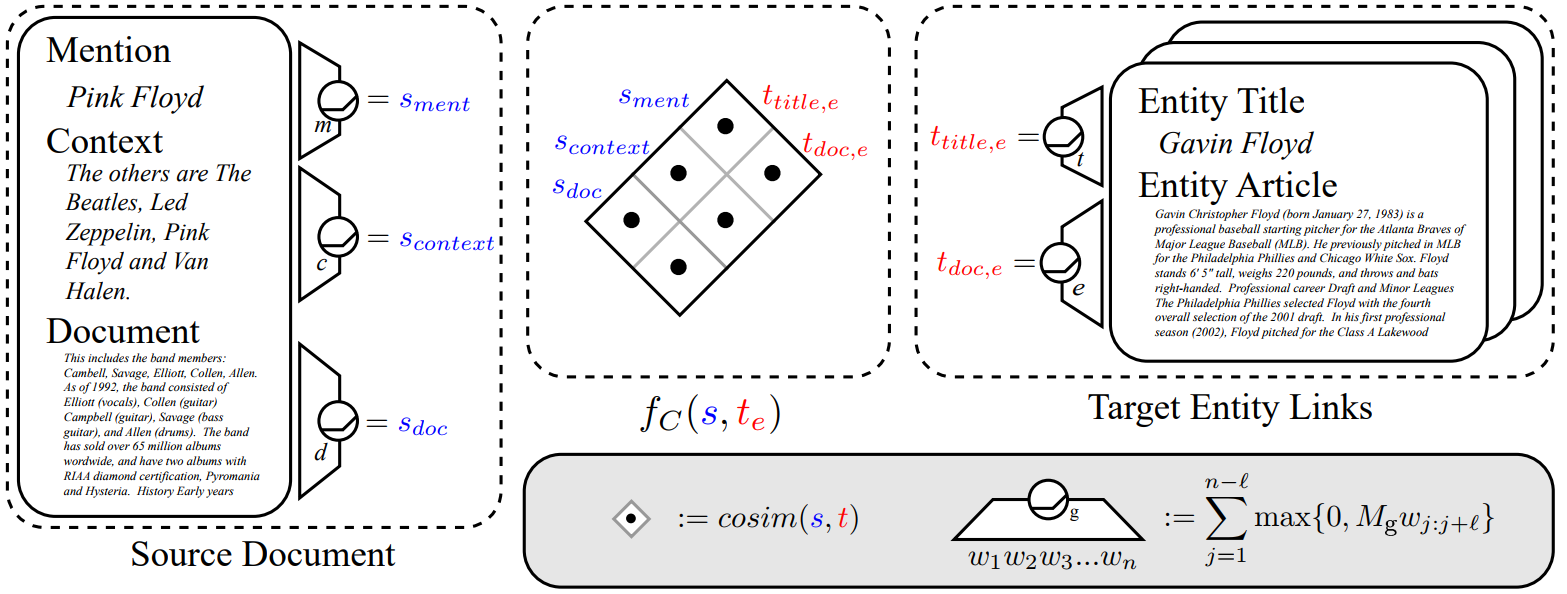
\includegraphics[width=0.95\columnwidth]{figure/rw/linking-francis.png}
	\bicaption{基于多粒度卷积神经网络的实体链接模型。\cite{francis2016capturing}}
    {Entity linking model with CNN at multiple granularities.}
	\label{fig:rw-linking-francis}
\end{figure}


%(68)[Pic][IJCAI] Modeling Mention, Context and Entity with Neural Networks for Entity Disambiguation (TAC-KBP数据集)
Sun等人\cite{sun2015modeling}的模型对不同的上下文信息
采用了不一样的网络结构。
如\figref{fig:rw-linking-sun}所示,
对短语建模的信息包括短语自身,以及去除自身后的句子两部分,
而实体方面,除了利用本身名称之外,还使用了它在维基百科中的分类信息,
用这类人工提炼的知识补充实体的表示。
对句子的表示学习依然使用卷积神经网络,
其余三种信息由于长度较短,均直接使用了词向量平均的方式得到向量表达。
进一步,该模型利用较为复杂的神经张量层将各部分向量结合,
分别得到实体和短语的整体表达。
%以捕捉向量不同维度间的信息交互。
类似的方法还有文献\parencite{gupta2017entity},
对实体的维基分类信息进行表示学习,
通过双向循环神经网络对短语所在句子进行编码。
同时模型定义了不同信息之间的多种损失函数,对训练数据的利用更加充分。
%(7)[Pic][EMNLP] Entity Linking via Joint Encoding of Types, Descriptions, and Context
%(6)[BadPic][COLING] Joint learning of local and global features for entity linking via neural networks (ref充数用,需要再加)

\begin{figure}[th]
	\centering
    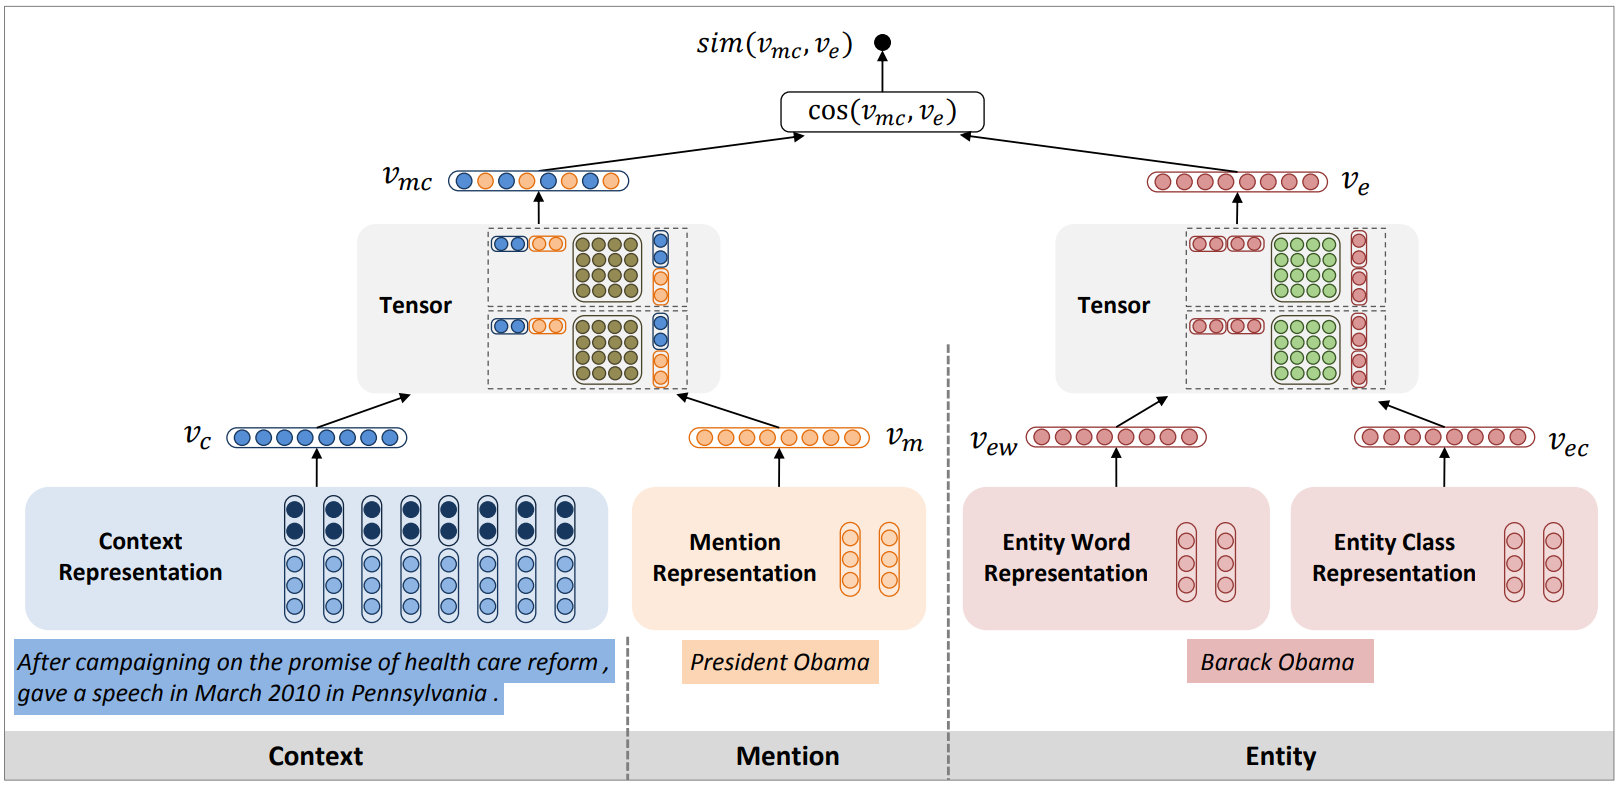
\includegraphics[width=0.95\columnwidth]{figure/rw/linking-sun.png}
	\bicaption{基于神经张量层的链接模型。\cite{sun2015modeling}}{NTN based entity linking model proposed by Sun et al.}
	\label{fig:rw-linking-sun}
\end{figure}

%(22)[NoPic][CoNLL] Entity Disambiguation by Knowledge and Text Jointly Embedding
此外,知识库向量学习技术\cite{bordes2013translating}也被用于实体链接任务中。
知识库向量学习与词向量学习类似,以大量事实三元组作为训练数据,
学习每个实体的向量表示,使得相近语义的实体具有相近的向量。
Fang等人\cite{fang2016entity}提出的链接模型基于知识库向量与词向量的融合:
通过实体与短语互相替代的方式,定义了基于三元组以及共现词对的目标函数,
促使实体与其短语的向量尽可能一致,因此所有向量表示被映射到同一个高维语义空间中。
融合的优势在于实体和单词之间直接可比,
通过距离度量函数计算候选实体与短语上下文中不同词的距离,
并以此作为链接模型的特征。

%(41)[NoPic][CoNLL] Joint Learning of the Embedding of Words and Entities for Named Entity Disambiguation(凑人头)
%(9)[Pic][EMNLP] Deep Joint Entity Disambiguation with Local Neural Attention(凑人头)


%"通过xxx得到xxx,因此可以对xxxx进行建模  进一步xxxx"



%出现在Tutorial里的
%Local and Global Algorithms for Disambiguation to Wikipedia (Ratinov)(Illinois Wikifier)
%Robust Disambiguation of Named Entities in Text (放图)(AIDA数据集)
%Linden: linking named entities with knowledge base via semantic knowledge
%Joint Named Entity Recognition and Disambiguation(EMNLP2015,CRF)(AIDA)
%S-MART(啥数据?)(啥特征?)
%不同特征对应的不同类型。



%\subsection{跨语言场景的实体链接模型}
%\label{sec:rw-linking-bilingual}


\subsection{跨语言词向量}
\label{sec:rw-linking-cle}

上一节的论述中提到了词向量模型,用于学习词汇的连续语义表示,但仅局限于单一语言。
对于涉及多个语言的任务,难点在于如何实现语义的跨语言过渡。
为了解决此问题,跨语言词向量模型(Cross-Lingual Embedding Model)
旨在消除单词语义表示对语言的依赖,
将不同语言的向量表示映射至同一连续空间,并依旧保持相似语义单词更加接近的特性,
以此实现语义迁移。
例如\figref{fig:rw-linking-cle}展示了一个英语和德语之间的共享语义空间,
可以清晰地识别出两种语言间的许多组翻译词对。

\begin{figure}[th]
	\centering
    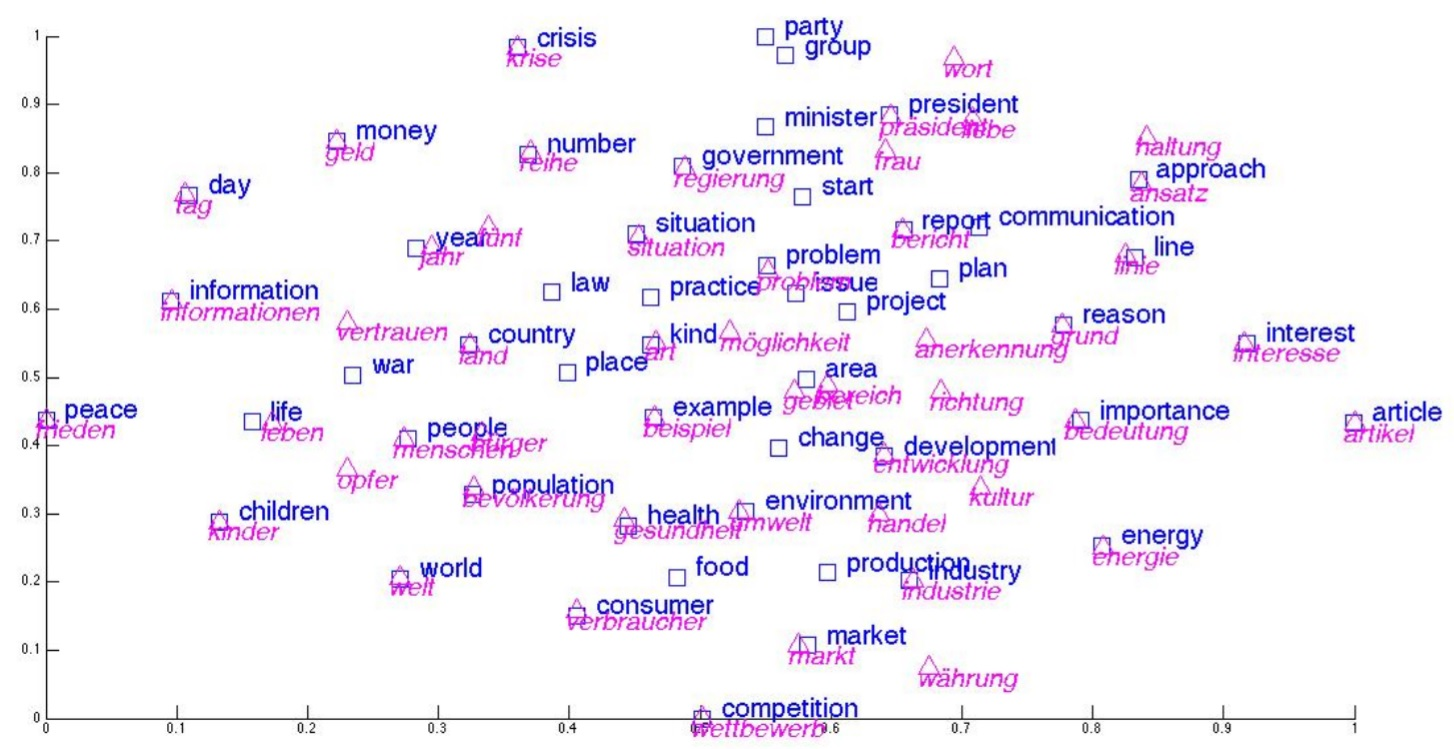
\includegraphics[width=0.8\columnwidth]{figure/rw/linking-cle.jpg}
	\bicaption{英语和德语间的跨语言词向量例子。\cite{ruder2017survey}}
    {An example of cross-lingual word embeddings between English and German.}
	\label{fig:rw-linking-cle}
\end{figure}

跨语言词向量的训练,需要依赖平行语料库用于给模型提供语义对齐信号,
不同的训练方式区别在于平行语料的类型不同,
例如单词级别\cite{mikolov2013exploiting,klementiev2012inducing,lazaridou2015hubness}、
句子级别\cite{hermann2013multilingual,gouws2015bilbowa}、
文档级别\cite{vulic2016bilingual}的对齐。
利用单词级别对齐进行跨语言词向量训练的工作最为普遍,
训练数据主要来自于双语或多语词典中抽取出的高质量翻译词对。
以此为例,对于源语言$s$和目标语言$t$,模型的损失函数$J$由三部分组成:
\begin{equation}
  J = \mathcal{L}_{mono}^{s} + \mathcal{L}_{mono}^{t} + \Omega{}^{s \rightarrow t},
\end{equation}
\noindent
其中,$\mathcal{L}_{mono}$代表各自语言上进行单语言词向量训练的损失,
可直接使用CBOW等已有模型进行计算,
而$\Omega{}^{s \rightarrow t}$为正则项,对应单词对齐的损失。


对于$\Omega{}^{s \rightarrow t}$的定义,相关文献进行了不同的尝试。
Mikolov等人\cite{mikolov2013exploiting}发现,
在不同语言中,多个单词的向量表达之间,几何关系较为相似,
例如英语和西班牙语中,表示数字的单词之间的相对位置几乎一致,
表示动物的单词也有类似特性。
基于以上观察,该工作提出的模型使用了线性变换的方案,
训练转移矩阵$\bm{W}$(或称投影矩阵),
使得源语言词向量$\bm{x}^{s}$经过$\bm{W}$投影后,和对齐的目标语言词向量$\bm{x}^{t}$
的欧氏距离平方(即均方误差)尽可能小:
\begin{equation}
  \Omega{}^{s \rightarrow t} = \sum_i { \| \bm{Wx}_i^s - \bm{x}_{i}^{t}  \|^{2} },
\end{equation}
\noindent
基于线性映射的跨语言词向量模型具有一些变种,
例如文献\parencite{xing2015normalized,zhang2016ten}限制转移矩阵$\bm{W}$为单位正交阵,
以保证映射后的词向量维持单位长度,
Artetxe等人\cite{artetxe2016learning}指出,对于模型效果而言,
转移矩阵正交化比向量正则化更加重要。
Lazaridou等人\cite{lazaridou2015hubness}对$\Omega{}^{s \rightarrow t}$的定义使用了最大间隔(Max Margin)损失
来代替均方误差损失,即不追求$\bm{Wx}^s$与$\bm{x}^t$绝对距离尽可能小,
而是让$\bm{x}^t$比其它任何不相关单词都更加接近$\bm{Wx}^s$,
从而避免跨语言词向量出现过多中枢词的现象。
Faruqui等人\cite{faruqui2014improving}利用
典型相关分析(Canonical Correlation Analysis, CCA)\cite{hotelling1936relations}
进行词向量训练。CCA同为线性投影方式,不同之处在于,
%也可用于将不同语言的词向量线性投影到同一个向量空间中,与之前的线性映射不同,
CCA对两个语言分别学习一个线性变换矩阵,
目标是尽可能降低映射后每个翻译词对的互协方差分值。

%训练过程:分开,joint
%(稍微扯一下优点,虽然还没想好)
此外,跨语言词向量的训练还可
对于通过句子或文档级别的平行语料进行跨语言词向量的训练,由于不是本文的研究重点,
故不展开论述。
跨语言词向量能够应用在多种任务中,
例如文档分类\cite{klementiev2012inducing}、词性标注\cite{zhang2016ten}、
命名实体识别\cite{murthy2016sharing}、机器翻译\cite{zou2013bilingual}等,
其带来的知识迁移具有很高的实用性。
对于训练集和测试集为不同语言的任务,跨语言词向量能实现知识在不同语言上的迁移;
对于类似机器翻译、跨语言实体链接等输入和输出为不同语言的任务,
预训练好的跨语言词向量能够作为特定任务模型的训练起点,
消除语义的间隔,从而提升整体效果。


%Zhang IJCAI 2012 Cross Lingual Entity Linking with Bilingual Topic Model

%Sil AAAI 2018 Neural Cross-Lingual Entity Linking (先放着,来不及了)
%Tsai NAACL 2016 Cross-lingual Wikification Using Multilingual Embeddings (留给小RW)


%Entity linking or wikification is another task tackled using cross-lingual word embeddings
%(Tsai & Roth, 2016). The purpose of the task is to ground mentions written in nonEnglish
%documents to entries in the English Wikipedia, facilitating the exploration and
%understanding of foreign texts without full-fledged translation systems (Ji, Nothman,
%Hachey, & Florian, 2015). Such wikifiers, i.e., entity linkers are a valuable component
%of several NLP and IR tasks across different domains (Mihalcea & Csomai, 2007; Cheng
%& Roth, 2013).







%# -*- coding: utf-8-unix -*-
% !TEX program = xelatex
% !TEX root = ../thesis.tex
% !TEX encoding = UTF-8 Unicode

\section{关系理解:知识库补全任务}
\label{sec:rw-kbc}

%Part 1: 什么是KBC

现有的知识库具包含了庞大数量的实体和事实,但其中的内容仍然不够完全,
尤其是存在大量的长尾实体,并没有多少事实与之相关。
因此,知识库补全任务(Knowledge Base Completion, KBC)的目的,
是向已有知识库中添加缺失的事实三元组($e_1$, $p$, $e_2$)。
这些新增的三元组中,无论是谓词$p$还是它的两个参数实体$e_1$和$e_2$,
都已存在于知识库中。
换言之,新增的事实并不会给知识库带来额外的节点,或是从没见过的边,
而是让知识库的图结构更加稠密。

新增事实三元组(尤其是参数实体)的获取方式通常有两种。
第一种来源为经过了实体链接过后的外部文本,纯文本或表格文本均可称为来源。
%
对于纯文本,当在句中定位两个参数实体后,
句子剩下的部分成为了描述实体间关系的上下文。
此时即可依据上下文信息来预测对应的知识库谓词,
即等价于关系分类问题,相关研究包括词级别卷积神经网络\cite{xu2015semantic}
以及依存语法路径上循环神经网络\cite{xu2015classifying}。
对于表格文本,知识库补全关注于表格的两列之间,利用表列所包含的实体,
判断两列之间的关系是否与知识库中特定谓词对应,实现可能的大批量事实补全。
例如\figref{fig:rw-linking-limaye},
Title和Author列之间的关系被映射到YAGO中的$Writes$谓词。
%主要使用的方法有
%如概述中指出,  表格关系可以补充三元组
%Munoz:找关系 挖掘不同行之间,但是是同样的两列之间的实体关系,映射至DBPedia 构成三元组,即挖掘语义。  并补充缺失
%在维基百科内部(已有链接)
%按已有match比例尝试一些predicate,然后学习一个triple是对还是错
%Sekhavat: Tabular KBC 同样是假设linking已好的情况 利用PATTY作为跳板,根据EP之间存在的pattern,寻找到rel的关系
%条件概率  (相当于EP有一系列的外部文本pattern,而不是仅有KB)
%rel来自YAGO
%(Fuck...但两者根本都是column-column-rel和predicate的一一对应)

第二种来源不涉及到任何知识库外的信息,新增三元组来自于知识库的内部挖掘,
通过寻找不同谓词之间的关联,推理出可能缺失的事实。
例如\secref{sec:intro-background}提到的例子,
``{某人的国籍缺失,可以根据其出生地所在的国家进行推测}'' ,
人类可以通过这样的方式进行知识的手动补充,正是因为掌握了
国籍、出生地、地点被包含这三个谓词之间的关联。
这条路线不受知识库外信息的干扰,因此是我们关注的研究点。

学术界已有工作在此场景上研究知识库补全的解决方案,
并提出了相关的KBC数据集,
例如FB15k\cite{bordes2013translating}和WN18\cite{bordes2014semantic},
分别是Freebase和WordNet的子集。
对于知识库补全模型的测评,主要通过
主宾语预测(Link Prediction)以及三元组分类(Triple Classification)
这两个子任务来进行。
前者为三元组($e_1$, $p$, $?$)或($?$, $p$, $e_2$)预测缺失的主语或宾语,
后者则判断给定的($e_1$, $p$, $e_2$)是否为正确事实。
两者虽然形式不同,但都需要计算三元组的置信分:$S(e_1, p, e_2; KB)$。

解决知识库补全的方法主要分为两类。
第一类基于规则推导,用逻辑表达式描述实体间存在特定谓词时,所需要满足的特定规则;
第二类基于知识库向量,学习所有实体、谓词的连续特征表示,
并挖掘三元组各部分特征表示之间存在的深层代数关系。
下面将分别介绍这两种方法。

\subsection{基于规则推导的模型} %基于规则推导的关系语义推理模型

基于规则推导的模型旨在使用人类可以直接理解的规则形式,来描述不同谓词之间的联系,
即如果$e_1$和$e_2$之间满足特定的条件,则推理出三元组($e_1$, $p$, $e_2$)成立。
为方便论述,我们将三元组以布尔表达式$p(e_1, e_2)$表示,
若对应三元组存在于知识库中,则表达式为真,否则表达式为假。
文献\parencite{lao2011random}以一个简单的推导规则为例:
若已知某运动员为球队效力,以及球队所处联盟,则可以推导出运动员所参与的体育联盟。
该规则可以通过一阶逻辑表达式进行形式化描述:
\begin{equation}
\begin{aligned}
\exists b \in E, athletePlaysForTeam(a, b) & \land teamPlaysInLeague(b, c) \\
                                           & \implies athletePlaysInLeague(a, c),
\end{aligned}
\end{equation}
\noindent
其中$E$表示知识库实体集合。规则的左侧部分,使用的两个谓词实现了主语$a$到宾语$c$的连接,
且不包含多余的布尔表达式,因此这条规则表现为由谓词序列构成的路径。
对于``{依靠出生地推测国籍}'' 的规则,我们可以形式化为以下逻辑表达式:
\begin{equation}
\begin{aligned}
  \exists b \in E, placeOfBirth(a, b) & \land containedBy(b, c) \\
                                      & \land isA(c, country) \implies nationality(a, c),
\end{aligned}
\end{equation}
\noindent
其中谓词序列$\{placeOfBirth, containedBy\}$为连接主宾语的路径,
而谓词$isA$使得宾语$c$还需要满足额外的限制条件,因此这条规则具有比路径更加复杂的结构。

利用单个推导规则进行知识库补全存在两个局限:
首先,规则本身不一定完全正确,限制条件过于宽泛的规则可能打来错误的事实;
其次,单个规则的覆盖率较低,能够补全的知识有限。
针对这两个局限,已有的规则推导工作都致力于从知识库中挖掘目标谓词的多条规则,
并学习不同规则的重要性,以实现更健壮的知识库补全。

Lao等人提出的PRA模型\cite{lao2010fast}实现了规则的挖掘和学习。
对于目标谓词$p$,模型首先利用谓词已有的三元组($e_1$, $p$, $e_2$)作为训练数据,
在知识库中寻找所有能连通$e_1$和$e_2$的谓词序列,形成了多种路径形式规则。
模型利用逻辑回归实现规则权重的训练,以及对新三元组($e'_1$, $p$, $e'_2$)是否为真的预测。
每一条挖掘的规则类比为一个特征,对应的特征值为路径随机游走概率,
即从主语$e'_1$出发,沿规则的谓词序列随意跳转,最后到达$e'_2$的概率。
由于知识库中的谓词可能代表一对多关系,
因此随机游走概率值会小于1,甚至为0(无法通过当前规则连通)。
基于此,PRA模型能够快速抽取大量路径规则,并利用已知三元组在规则上随机游走概率实现权重训练。

一些研究工作对PRA模型进行了扩展。
文献\parencite{lao2011random}对挖掘的路径规则进行了限制,
要求规则至少要适用于训练数据中一定比例的主语,并对计算随机游走概率的采样方式进行了优化,
这两个扩展都是基于模型性能优化为考量。
%lao2011random
%改进1: 限制每条路径规则所能  满足的主语个数  以及连通的 训练三元组个数,  大幅度缩小规则数量
%改进2:随机游走的采样方式进行了优化。
Gardner等人提出了SFE模型\cite{gardner2015efficient},它在PRA模型基础上进行了两项改进:
首先,模型将作为特征值的随机游走概率替换为0/1特征,即只关心是否连通,
在大幅度提升运行速度的同时,对结果没有显著影响;
其次,模型引入不同于路径规则的其它特征,例如提取路径中的谓词bigram,
或由主语出发却不指向宾语的单边特征等,扩充特征集合以提升知识库补全效果。
%gardner2015efficient
%改进1:特征值转换为0/1对结果没有显著影响,PRA的具体概率值并不比0/1提供了更多信息(很惊讶),而PRA概率计算花费了大量时间
%改进2:引入了更多的规则,单边  anyrel, path bigram   并非基于路径的规则 but useful
Wang等人提出了CPRA模型\cite{wang2016knowledge},主要针对具有相似谓词的规则推导优化。
该模型通过层次聚类识别出具有相似语义的知识库谓词集合,
然后对每个集合内的谓词采用多任务学习框架,共享挖掘的规则特征和部分耦合参数,
使模型能够捕捉相似谓词之间的共性,实现隐式的训练数据共享。
%wang2016knowledge
%针对具有相似语义的知识库谓词,对它们的关系推理 过程   不独立,而是 能 彼此利用训练数据  互相影响,
%提出了  CPRA模型,   通过层次cluster识别  相似语义 的知识库谓词 ,   多任务学习 等方式 学习,
%使得  不同谓词的规则推导 不完全独立,   可以利用其它 的训练数据  优化自身。

%TODO: AMIE+, Zhang的放在内部related work说,有点太细了
% AMIE+
% 
% Zhang等人的研究 是 此任务 较早的工作。
% 文中称Ontological Smoothing, 为 特定关系寻找更多seed pair,
% 并用于relation extraction中,以提高pattern的准确率。
% 虽并不称作kbc,但本质相同。
% 提出了基于MLN的模型。
% 不仅
% 对每个谓词生成的规则由长度不超过4的谓词序列
% 同时对NELL 中的e和t都映射
% 
% 使用MLN学习每个规则的权重
% 对每个 谓词 相关规则   都寻找  合适的表达式,   谓词序列  考虑 并集
% 
% (类似的文章还有SQL query generation,见他的RW)
% 
% Zhang,MLN。。。
% %说各自的弱点
%   title={Learning to refine an automatically extracted knowledge base using markov logic},
%     goal: 过滤NELL,在candidate facts里寻找正确的fact。
%     rules: 好像并没有直接去学习p和p之间的关联,而是和meta predicate在搞?
%     model: MLN
%     
%   title={Large-scale knowledge graph identification using psl},
%     goal: 同上
%     rules: extractor, ontological, isA, relation
%     model: PSL, weight on rule, and also on the atom expression (KALE)
% 
%   title={Statistical schema induction},
%     太长了,先忽略
% 
% 
% 然后就终结在这里。不要再多了,ball ball u.

\subsection{基于知识库向量的模型}

与词向量模型类似,知识库向量的模型旨在学习一个知识库中的实体、谓词等元素
在连续空间的特征表达,以完成一系列下游任务。
具体在知识库补全任务中,
三元组置信分的计算并不依赖自动挖掘的推导规则,
而是来自主谓宾三者的连续特征表达在不同维度上的交互。
词向量模型依靠大规模的纯文本语料,
构建上下文单词预测任务来完成训练\cite{mikolov2013exploiting},
相比之下,知识库向量模型的训练过程更为直观:
利用知识库已有三元组作为训练数据正样本,
并自动生成不存在的三元组作为负样本,计算三元组置信分进行训练,
而这也恰好与知识库补全任务的目标一致。

知识库向量模型的优点在于所有谓词共同训练,更有效地利用训练数据,
并且能在连续空间中体现不同谓词的相似性,
但相应地,其缺点在于可解释性较弱。
不同的知识库向量模型对实体和谓词的特征表示具有不同的形式,
特征交互的方式也不尽相同,下面主要介绍几个具有代表性的模型。
%一类以RESCAL为代表,多层网络输出multi-layer perc;一类以TransE为代表,latent distance model

%类比词向量的训练,CBOW 等 依据上下文进行预测,相似语义 相似上下文
%类似的思路,信息来自已有的事实三元组,相似的实体 会有相似的谓词和另一个实体
%对于谓词也有类似的性质
%然而,上下文信息由三元组表示,准备好了更加准确的训练数据。
%以及实体和谓词并不是同一类东西,不能像word2vec那样,实体和谓词会在不同的空间中。
%From: A review of relational machine learning for knowledge graphs


\begin{figure}[htp]
  \centering
  \subcaptionbox{RESCAL模型\label{fig:rw-kbe:a}}
    {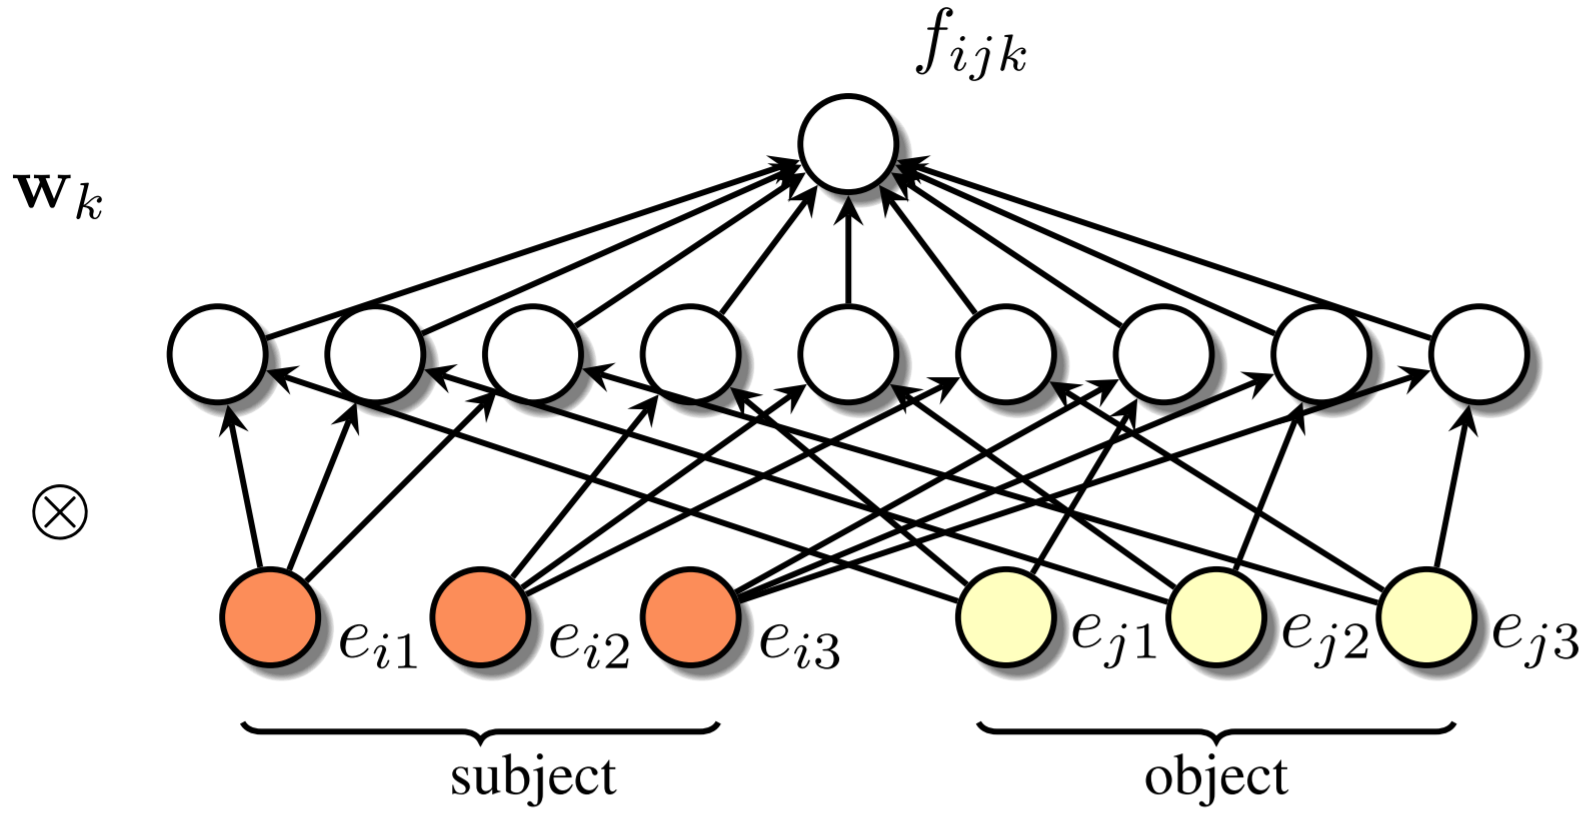
\includegraphics[width=0.48\columnwidth]{figure/rw/kbc-rescal.png}}
  \hspace{1em}
  \subcaptionbox{ER-MLP模型\label{fig:rw-kbe:b}}
    {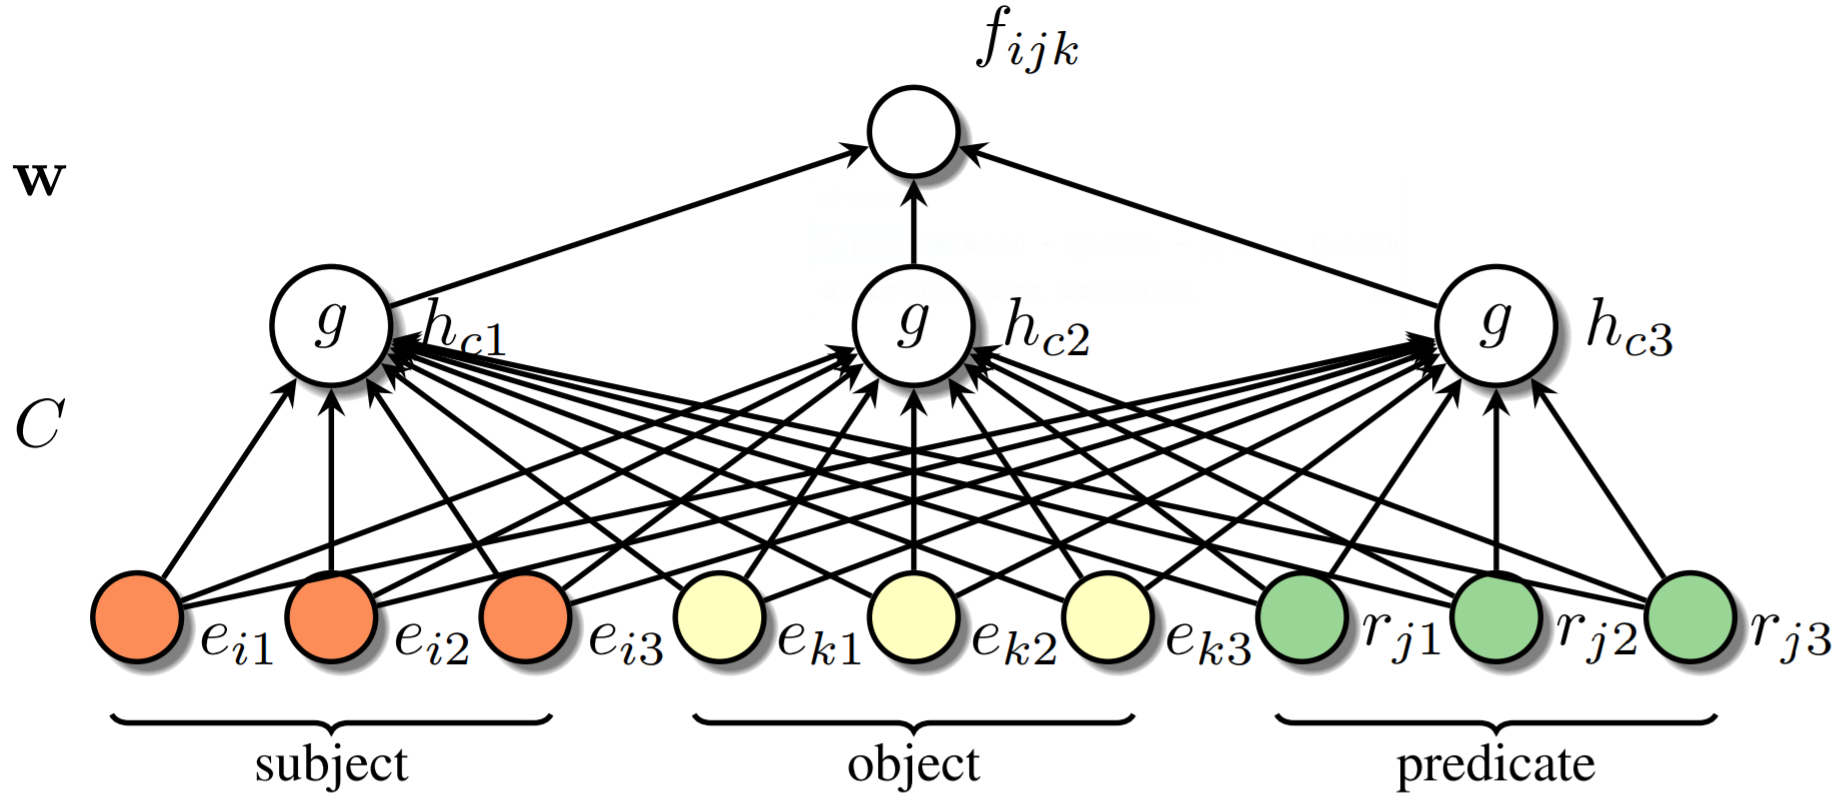
\includegraphics[width=0.48\columnwidth]{figure/rw/kbc-ermlp.png}}

  \vspace{1em}

  \subcaptionbox{TransE模型\label{fig:rw-kbe:c}}
    {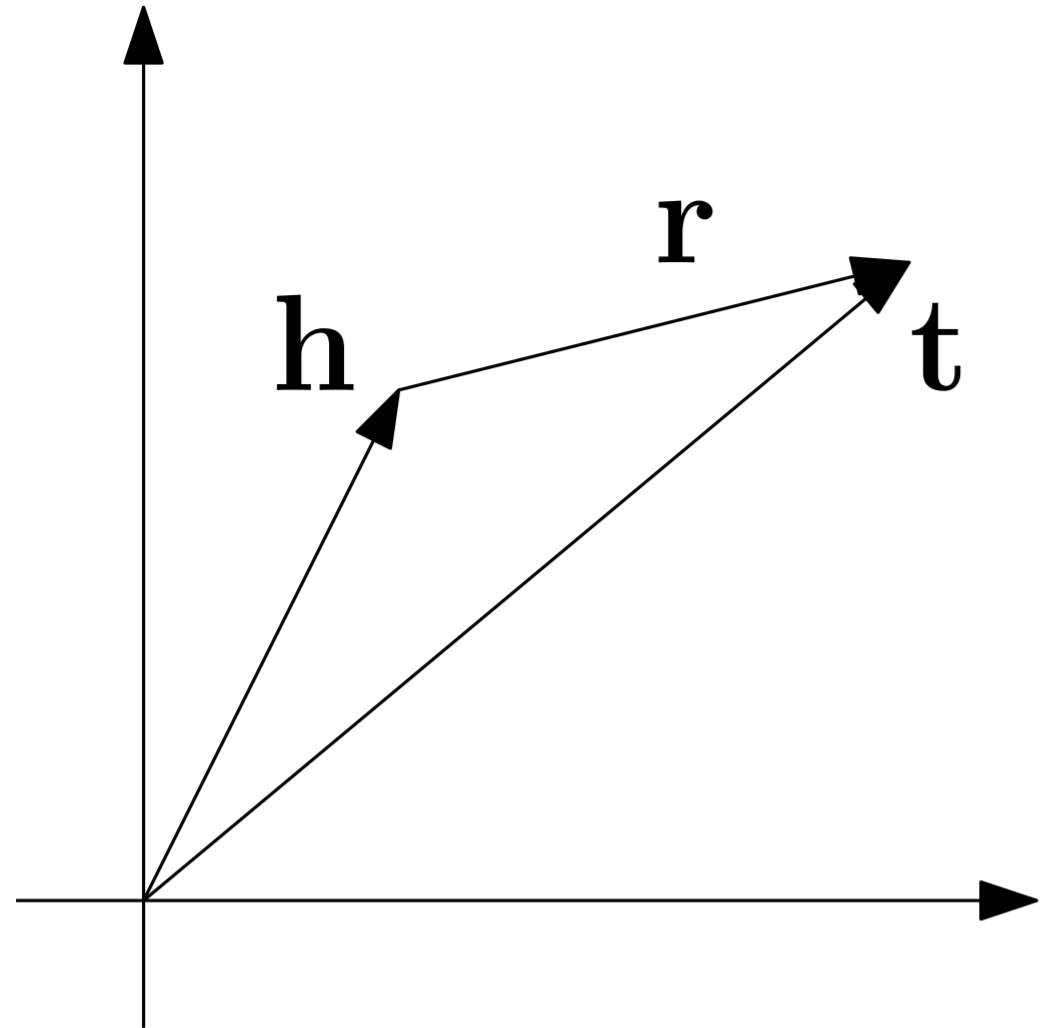
\includegraphics[width=0.30\columnwidth]{figure/rw/kbc-transe.png}}
  \hspace{4em}
  \subcaptionbox{TransH模型\label{fig:rw-kbe:d}}
    {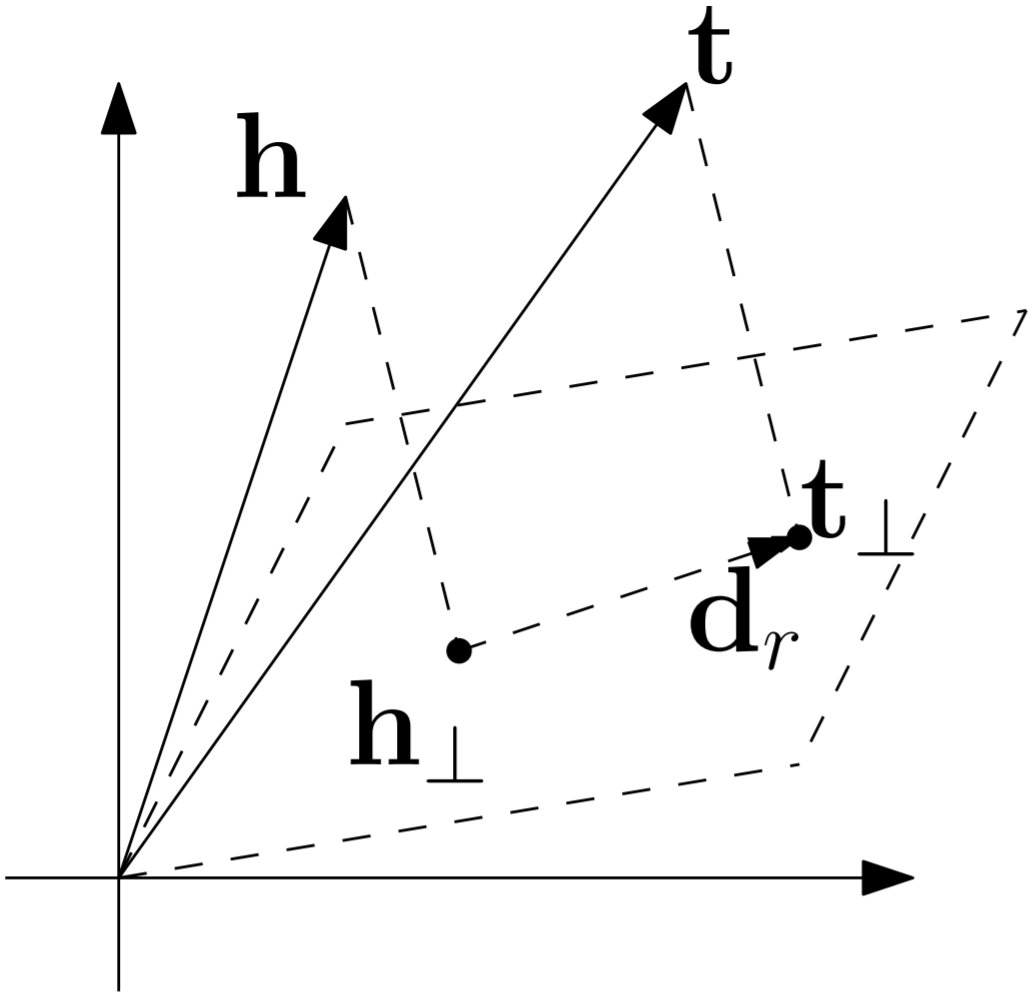
\includegraphics[width=0.30\columnwidth]{figure/rw/kbc-transh.png}}
  \bicaption{多种知识库向量模型示意图。\cite{nickel2016review,wang2014knowledge}}
            {Examples of knowledge base embedding models.}
  \label{fig:rw-kbe}
\end{figure}


由Nickel等人提出的RESCAL模型\cite{nickel2012factorizing}是一个基础的知识库向量模型,
模型对三元组($e_i$, $r_k$, $e_j$)置信分(简写为$S$)的定义,
基于主宾语实体特征表示的在不同维度间的两两交互:
\begin{equation}
S^{RESCAL} = \bm{e}_i^\top \bm{W}_k \bm{e}_j = \sum_{a=1}^d \sum_{b=1}^d w_{kab} e_{ia} e_{jb},
\end{equation}
\noindent
其中$\bm{e}_i$和$\bm{e}_j$为对应实体向量,维度为$d$。$\bm{W}_k \in \mathbb{R}^{d \times d}$
为谓词$r_k$的权重矩阵,其中$w_{kab}$体现了实体向量的第$i$和$j$维特征对于第$k$个谓词的交互重要性。
由于RESCAL使用矩阵连乘形式捕捉实体向量之间的交互,因此也被称为双线性模型。
如\figref{fig:rw-kbe:a}所示,RESCAL模型可表示为双层神经网络结构,
首先通过张量积(Tensor Product)构建实体对($e_i$, $e_j$)的组合特征,
再利用与特定谓词相关的参数$\bm{W}_k$作为权重,得到三元组最终的置信分。
RESCAL模型学习的实体特征表示能够捕捉不同实体间的语义相似性,
换言之,若两个实体可以通过相似的谓词连接至相似的其它实体,
那么它们的特征表达也更加相近。

%The shared entity representations
%in RESCAL capture also the similarity of entities in the
%relational domain, i.e., that entities are similar if they are
%connected to similar entities via similar relations [65].


RESCAL模型存在的一个问题在于参数量过大,每一个谓词对应参数量为$d \times d$,
对于拥有大量谓词的知识库而言,会带来可扩展性的问题。
一些后续研究对此进行了改进。
Socher等人以及Dong等人
分别提出了E-MLP\cite{socher2013reasoning}和ER-MLP模型\cite{dong2014knowledge}。
\figref{fig:rw-kbe:b}为ER-MLP的示意图,均由两层前向网络构成,
第一层用于学习三元组的组合特征表示,第二层则通过组合特征输出置信分。
E-MLP结构较为类似,故此处不专门画图。
两个模型的置信分计算如下:
\begin{equation}
\begin{aligned}
& S^{E-MLP} = \bm{w}_k^\top \bm{g}(\bm{C}_k [\bm{e}_i; \bm{e}_j]), \\
& S^{ER-MLP} = \bm{w}^\top \bm{g}(\bm{C} [\bm{e}_i; \bm{e}_j; \bm{r}_k]),
\end{aligned}
\end{equation}
\noindent
其中,$g$为非线性激活函数。
对比RESCAL模型,E-MLP的最大不同在于可以通过调整矩阵$\bm{C}_k$来学习实体间不同维度特征的交互,
从而优化实体对($e_i$, $e_j$)的组合特征表示,并大幅度减少参数数量。
E-MLP模型中,不同的谓词依然对应不同的参数,而ER-MLP模型将谓词也映射为向量表示,
与两实体共同作为第一层的输入,因此模型的参数$\bm{C}$与$\bm{w}$均与特定谓词无关。
两个模型依然能够让语义相似的实体映射至连续空间的相近位置。

Nickel等人提出了HOLE模型\cite{nickel2015holographic},
该模型利用循环相关运算(Circular Correlation)巧妙地代替了RESCAL中的张量积操作:
\begin{equation}
S^{HOLE} = \bm{w}_k^\top (\bm{e}_i \star \bm{e}_j) = \sum_{a=1}^d \sum_{b=0}^{d-1} w_{ka} e_{ia} e_{j,(a+b) \% d},
\end{equation}
\noindent
可以从公式中看出,循环相关运算等同于将张量积的结果进行了分组,模型通过对实体特征表示的学习,
让具有相似语义的特征交互归为同一组,共享同一个权重。
因此HOLE的优势在于将RESCAL中的二维矩阵参数降低至一维,同时尽可能保留了特征交互的表示能力,
并且在实验中效果优于RESCAL和ER-MLP模型。

此外,Socher等人还提出了较复杂的神经张量网络(Neural Tensor Networks,NTN)模型\cite{socher2013reasoning},
可以看做是RESCAL和E-MLP的组合体,对实体对($e_i$, $e_j$)构建的组合特征表达同时包括双线性和前向网络特征,
但模型参数量也因此更加庞大,在小数据集上更容易出现过拟合。



%1+3+1段
另一类 知识库向量模型   是以TransE为典型的 被称作 隐距离模型。
相比 RESCAL等模型 依照神经网络构建的置信分函数,
隐距离模型对置信分的计算则与距离度量直接相关。
这与\secref{sec:rw-linking-cle}介绍的跨语言词向量训练有着相似之处,
源语言词向量经过转换后,与翻译后的词向量尽可能相近。
而对于知识库向量模型,由于三元组中还有谓词的存在,
因此模型训练的实质,是学习主宾语实体向量在特定谓词下的变换方式,
对变换之后的向量表示进行距离度量,距离越近,则置信分越高。
为了和相关工作统一,此处用($h$, $r$, $t$)表示一个事实三元组。

Bordes等人提出的SE模型\cite{bordes2011learning}较为基本,
度量实体$h$和$t$经矩阵变换后的距离:
\begin{equation}
S^{SE} = -dist(\bm{A}_r^s \bm{h}, \bm{A}_r^o \bm{t}),
\end{equation}
\noindent
其中$dist(\cdot)$为距离度量函数,例如L1距离或欧氏距离。
谓词$r$对应两个参数矩阵,分别映射主语和宾语实体的向量表示至同一空间。
为了降低参数个数,Bordes等人提出了TransE模型\cite{bordes2013translating},
这也是后续很多改进模型的起点。
受到词向量之间代数运算的启发,
例如$queen \simeq king - man + woman$\cite{mikolov2013linguistic},
不同词之间的关系体现在了它们词向量的位置偏移中,
因此如\figref{fig:rw-kbe:c}所示,TransE模型共享了实体与谓词的特征表示,
利用在主语实体在同一空间中的平移变换,代替更加复杂的矩阵变换:
\begin{equation}
S^{TransE} = -dist(\bm{h} + \bm{r}, \bm{t} ).
\end{equation}

TransE模型设计简单、容易实现,并且具有训练速度快、可扩展性高等优点,
但是对于知识库中存在的一对多或多对一的谓词不友好,
例如固定主谓,TransE无法有效区分出多个匹配的宾语实体。
为此,TransH模型\cite{wang2014knowledge}尝试通过超平面投影来解决此问题,
公式定义如下:
\begin{equation}
  \bm{h}_\bot = \bm{h} - \bm{w}_r^\top \bm{h} \bm{w}_r, \ 
  \bm{t}_\bot = \bm{t} - \bm{w}_r^\top \bm{t} \bm{w}_r, \
  S^{TransH} = -dist(\bm{h}_\bot + \bm{d}_r, \bm{t}_\bot),
\end{equation}
\noindent
如\figref{fig:rw-kbe:d}所示,TransH首先把$h$和$t$的向量表示均投影到连续空间中,
谓词$r$对应的超平面上($\bm{w}_r$为单位法向量),
并学习谓词向量表示$\bm{d}_r$,在超平面上沿用TransE的度量。
因此,TransH具有更高的灵活度来应对一对多或多对一谓词,
同时依然保有TransE可扩展性高的特点。
TransR模型\cite{lin2015learning}同样尝试解决一对多谓词的问题,
类似于SE和TransE的组合体,利用投影矩阵$\bm{M}_r$将实体表示转移至新的空间后,
再进行基于平移的距离度量。
因此TransR模型中,实体和谓词的特征表达并不共享同一个语义空间,
这与TransE和TransH模型均不同:
\begin{equation}
S^{TransR} = -dist(\bm{M}_r \bm{h} + \bm{r}, \bm{M}_r \bm{t}).
\end{equation}

此外,还有其它TransE模型的改进工作,
包括体现距离度量在不同特征维度间差异的TransA\cite{xiao2015transa},
生成谓词多个表示以解决一对多问题的TransG\cite{xiao2016transg}等,这里不再展开讨论。

   %关系语义推理,别叫知识库补全
%# -*- coding: utf-8-unix -*-
% !TEX program = xelatex
% !TEX root = ../thesis.tex
% !TEX encoding = UTF-8 Unicode

\section{问句理解:知识库自动问答任务}
\label{sec:rw-qa}


自动问答任务是一类以自然语言问句为输入,并自动给出对应答案的任务。
基于知识库的自动问答(Knowledge Base Question Answering, KBQA)
是其中的一个热门研究方向,也是本文重点关注的问题。
在此问答任务中,输入问句为来自开放领域的事实类问句(Factoid Question),
即问句本身描述的是与某些特定实体相关的客观事实,
对应的答案通常表示为知识库中的实体、时间、数值等简单形式,
因此类似 ``how'' ``why'' 等以完整句子作为答案,或事实涉及到主观判断的问题,
不在任务的考虑范围之内。
以一个简单的英文问句为例,问句 ``what state borders texas?''
描述了与德克萨斯州相关的事实,其答案有多个,
包括New Mexico,Oklahoma,Arkansas,以及Louisiana四个实体。

对于知识库问答任务,使用的外部信息显然为结构化知识库。
正确答案的获取依赖于问答模型对问句整体语义的理解:
一方面准确定位问句中出现的相关实体,并链接至知识库;
另一方面根据问句信息,推理出未知答案与相关实体在知识库中具有的关系。
前者涉及到实体链接技术,后者体现了问句与知识库的语义匹配,也是问答模型的核心。
为了衡量问答模型对不同类型问题的效果,
学术界已提出了大量知识库问答数据集,
例如对问句进行结构化语义标注的QALD\cite{cimiano2013multilingual}和Free917\cite{cai2013large},
以及具有更大规模问答数据量的WebQuestions\cite{berant2013semantic}
和SimpleQuestions\cite{bordes2015large}等。

%和检索式问答  相比, 知识库问答    两者最大的差别在于答案来源  外部信息  的不同。
%对于检索式问答   以Squad为例
%对比检索式问答,   答案来自于给定的  文本,  抽取出   答案片段;

与知识库补全任务类似,根据问句语义的表示形式进行划分,
知识库问答模型大致可以分为两类,
即基于语义解析(Semantic Parsing)和基于信息抽取(Information Retrieval)的模型,
下面将分别介绍研究。


\subsection{基于语义解析的问答模型}

解释语义解析技术之前,我们先讨论人类对问题的思考方式。
对于人类来说,问句 ``what state borders texas'' 包含了两个与正确答案相关的线索:
1) 答案是一个(美国的)州;
2) 答案与德克萨斯州相邻接。
由于答案未知,因此每一个线索都对应着一个具有变量参数的事实三元组。
语义解析技术的目的,就是用存在于知识库上的实体和谓词,
对这些线索进行结构化表示。
根据这两条线索,原问题的答案集合可表示为一阶逻辑表达式:
\begin{equation}
\label{eqn:logic-form}
AnswerSet(q) = \{x~ |~ IsA(x, US\_State) \land adjoin(x, Texas)\},
\end{equation}
其中$x$代表未知答案实体,表达式中的$p(x, y)$为真,当且仅当三元组($x$, $p$, $y$)存在于知识库中。
对于机器而言,得到逻辑表达式之后,将其翻译为知识库上的查询语句,
即可直接得到所有满足语义的答案,这些答案彼此具有完全一致的特征。

由此可见,基于语义解析的自动问答模型,
实质是寻找正确的语义结构化表示,
即判断\textless 问题,结构化语义 \textgreater 的匹配程度,
而不仅仅寻找一个答案实体。
相关工作
\parencite{kwiatkowski2013scaling,berant2013semantic,yih2015semantic,bao2016constraint}
的研究重点在于,如何由句子生成知识库上的结构化语义表示,
以及如何对问题和语义结构的匹配程度进行建模。


\subsubsection{结构化语义生成方法}   %文字1页,图0.25-0.5

%TODO: SPARQL什么时候提
%TODO: 什么地方提及它们的共性(logical form,以及限制种类)

仍以``what state borders texas'' 为例,
不同研究工作中的结构化语义形式并不相同,
但本质都为\eqnref{eqn:logic-form}所描述的逻辑表达式。
\figref{fig:rw-spt}列出了一些典型工作生成的解析结构。

\begin{figure}[!htp]
  \centering
  \subcaptionbox{成分解析树\label{fig:rw-spt:a}}
    {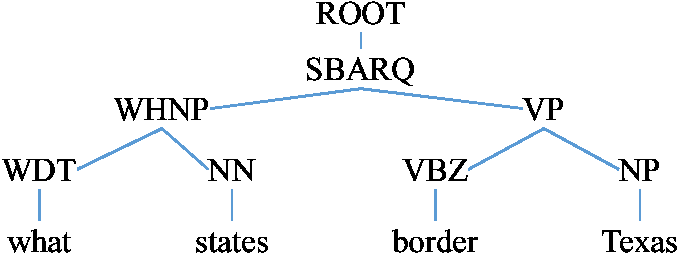
\includegraphics[width=0.48\columnwidth]{figure/rw/qa-parsing-xs.eps}}
  \hspace{1em}
  \subcaptionbox{基于PCCG的语义解析树\cite{zettlemoyer2012learning}\label{fig:rw-spt:b}}
    {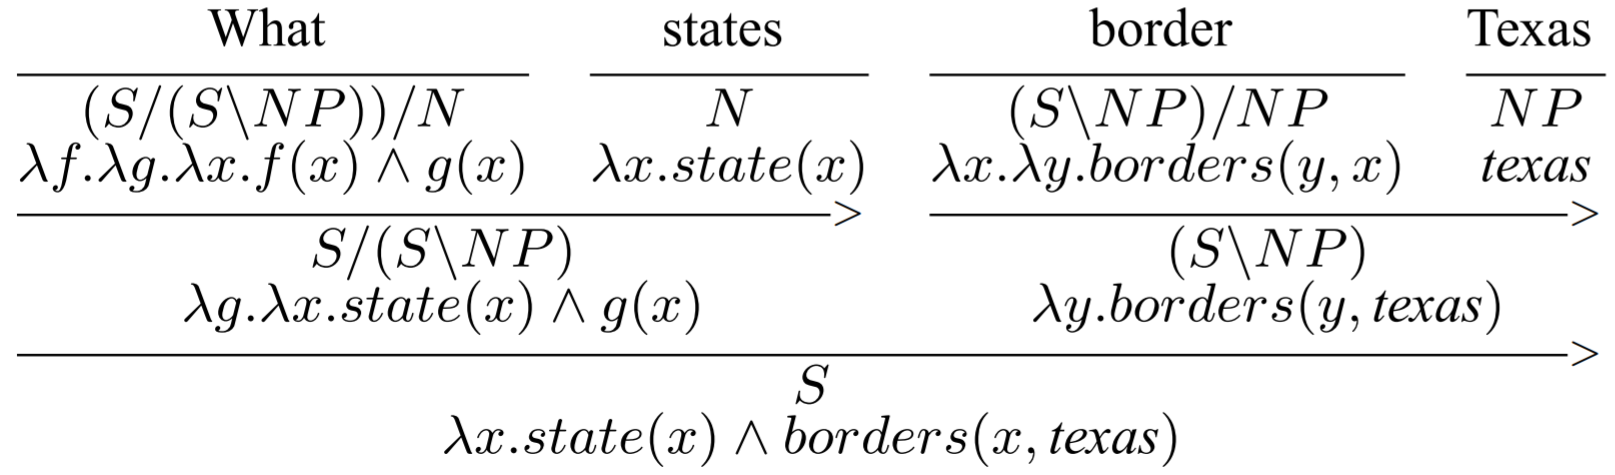
\includegraphics[width=0.48\columnwidth]{figure/rw/qa-ccg-3.png}}

  \vspace{1em}

  \subcaptionbox{基于$\lambda$-DCS的语义解析树\label{fig:rw-spt:c}}
    {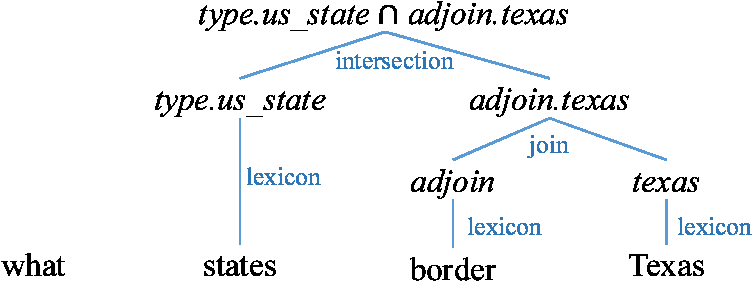
\includegraphics[width=0.48\columnwidth]{figure/rw/qa-dcs-xs.eps}}
  \hspace{3em}
  \subcaptionbox{基于多阶段生成的查询结构\label{fig:rw-spt:d}}
    {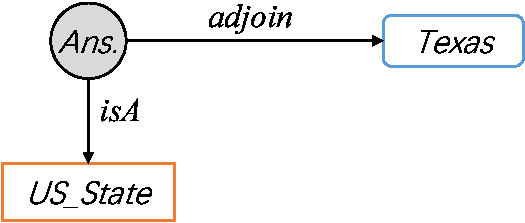
\includegraphics[width=0.38\columnwidth]{figure/rw/qa-stagg-xs.eps}}
  \bicaption{例句 ``what state borders texas'' 的多种解析结构。}
            {Several parsing structures for the question ``what state borders texas''.}
  \label{fig:rw-spt}
\end{figure}

%kwiatkowski2010inducing
%CCG cite
早期的语义解析模型\cite{zettlemoyer2012learning,kwiatkowski2010inducing,cai2013large}
使用概率化组合文法  (Probabilistic Combinatory Categorial Grammar,PCCG)
生成语义解析树。
该方法与语法解析中的概率化上下文无关文法(Probabilistic Context-Free Grammar,PCFG)相似,
根据训练数据学习文法中不同生成式规则的概率值,
并自底向上推理出每个句子最可能生成的成分解析树(Constituency Parsing Tree)。
\figref{fig:rw-spt:a}为例句的成分解析树,描述了整句的语法结构,
并标出了不同短语在句中的成分。
通过PCCG生成的语义解析树如\figref{fig:rw-spt:b}所示,
PCCG的生成式规则中不仅具有代表语法的成分信息,
同时还包含代表语义的$\lambda$表达式,
因此不同成分按照语法规则组合的过程中,
各自$\lambda$表达式也在进行拼接,从而得到对应整句话语义的逻辑表示。
PCCG语法具有很强的语义表示能力,
但由于生成式规则中涉及到不同的$\lambda$表达式,
同时训练数据匮乏,使得模型的训练具有难度。

% CCG: 语法以及语义,用lambda表达式来描述,
% 例如Inducing Probabilistic CCG Grammars from Logical Form
% with Higher-Order Unification
% 的例子,borders的那个
% 不仅语法组合成更高级的结构,语义也具有lambda表达式中的传参
% 
% PCCG: 同样概率介入,因为有多种合并方式。
% (lexicon怎么建,还要涉及词组)
% 特点:完全自底向上,每一个词都有用处(但是不是把问题搞复杂了)
% 可以支持很多操作,例如max、min、order等语义。
% 以及on-the-fly,语义解析树还需要一步转换,定位到特定的KB。


Liang在2013年提出的$\lambda$-DCS\cite{liang2013lambda}
旨在以更加简单的概念和流程,将问句转换为Freebase上的语义解析树。
如\figref{fig:rw-spt:c}所示,生成过程依然是自底向上模式,
叶节点(单词或词组)对应Freebase中的实体、类型或谓词,
但不再具有显式且复杂的$\lambda$表达式。
$\lambda$-DCS定义了节点组合过程的有限种语义合并方式,
包括连接、交集、并集甚至更加高阶的最值、计数等操作,
使得与PCCG相比,
生成的语义解析树在结构更加简单的同时,
牺牲了一定表达能力,
但对于事实类问题的理解来说依然足够。

Yih等人\cite{yih2015semantic}提出了一种多阶段的语义结构生成方法,
如\figref{fig:rw-spt:d}所示,语义解析树被表示为有向图形式,称为查询图,
图中的每一条边以及连接的两个节点,都对应\eqnref{eqn:logic-form}中的三元组。
与之前两种方法的自底向上生成不同,
多阶段语义结构生成基于由简到繁,逐步生成查询图的思路。
最简单的查询图为答案节点通过谓词(或多个谓词构成的序列)连接至
问句中的某一实体,形成仅有一条有向路径构成的查询图。
问句中抽取的其它实体、类型、时间等信息,则通过多个不同的阶段,
逐步连接至已有的路径上,构成更加复杂的查询图。
该方法不受限与问句中词的先后顺序,查询图的生成更加灵活,
在多个问答数据集上均有良好的效果。

Cui等人\cite{cui2017kbqa}提出了一种基于模板的方式,
对问句生成谓词序列形式的语义结构。
模板是对问句抽象表示,它将问句中的实体替换成类型,指代了一组具有相同语法和语义描述的问句,
``what states border \textit{\$location}'' 是一个具体的模板例子。
模板的提取依靠外部的大规模问答数据,
作者对Yahoo! Answers中大约41M问答对进行实体与答案识别后,
生成了约27M不同的模板,并通过EM算法学习其指向谓词序列的条件概率。
对于每一个问句的语义结构生成,则通过生成模型,由模板进行过渡得到不同谓词序列的概率。
这样的方法,优点在于利用大量外部数据获取准确率高的模板以及和语义的匹配,
但模型的召回率可能成为短板,当问句语法不规范时,简单的模板匹配容易失效。
%此外,其它的语义解析结构的生成方式,
%例如基于固定模板的结构生成\parencite{bast2015more,cui2017kbqa},
此外,一些文献\parencite{reddy2016transforming,hu2018answering}
使用了基于依存语法树转换的方式,利用结构相似性实现语义解析结构的生成,
这里不再一一介绍。


\subsubsection{语义匹配模型构建}    %文字1页,图0.25-0.5

由于自然语言的多义性,语义解析结构的生成结果通常都不唯一,
%因此模型需要计算问句与语义结构之间的匹配度,并根据问答数据进行训练。
%排名问题
因此需要对\textless 问句,语义解析结构 \textgreater 的匹配度进行建模,
选择最高匹配度的解析结构进行知识库上的答案查询。
%就三段,别多了
传统的语义解析模型主要基于特征工程,
Berant等人\cite{berant2013semantic}的研究工作为一个典型例子。
语义解析树由$\lambda$-DCS生成,
抽取出的特征包含三类:
问句中的短语与对应知识库谓词的对齐特征,
不同谓词参与合并的特征,
以及解析树的总体结构特征。
前两类特征来自于解析树的自底向上生成过程,用于捕捉每一个操作,
后一类特征则统计解析树中不同类型操作的数量,以及最终返回的答案数量。
%Kwai Cai Berant Bast
%基于特征工程的模型将解析树的生成看做操作序列,

为了弥补特征工程耗费人力的缺陷,同时获取更高层面的语义匹配信号,
Berant等人在后续的工作\parencite{berant2014semantic}中引入了转述特征(Paraphrasing Feature),
通过简单的规则将解析树翻译成自然语言问句,
并衡量原问句和生成问句之间是否具有转述关系,将其作为额外一组特征。
转述关系涉及到自然语言文本匹配问题,
作者使用基于词对应的关联模型和词向量的维度空间模型两种方式进行建模,
使得问答系统可以得到解析树的整体语义,是传统特征工程的有力补充。

最新的自动问答模型广泛使用了深度学习技术。
相关研究的共同点在于遵循一种 ``{编码—比较}'' 框架,
其重点在于,通过神经网络的特征学习能力,
对问句和解析结构分别进行编码,得到各自向量表示,
最后计算向量之间的相似度,代表问句与解析结构的匹配程度。
以简单问题数据集SimpQuestions为代表的问答模型几乎完全属于这一范畴,
由于在SimpleQuestions中,问句的语义解析结构均为单一谓词序列,
因此这些模型本质上都是对文本序列和谓词序列之间的匹配进行建模。
Yu等人\cite{yu2017improved}提出的HR-BiLSTM模型利用循环神经网络进行建模,
如\figref{fig:rw-siamese:a}所示,
谓词序列输入分为两个粒度:以唯一编号表示的编号序列,以及将谓词名称相连的单词序列,
分别通过双向LSTM层进行编码,
问句文本的编码也利用了双向LSTM层,并使用多层间的残差连接方式进行编码,
旨在让模型能同时捕捉单词粒度和问句整体粒度的语义信号。
SimpleQuestions上的其它类似模型还包括
文献\parencite{lukovnikov2017neural,yin2016simple,golub2016character,qu2018question}。

\begin{figure}[ht]
\centering
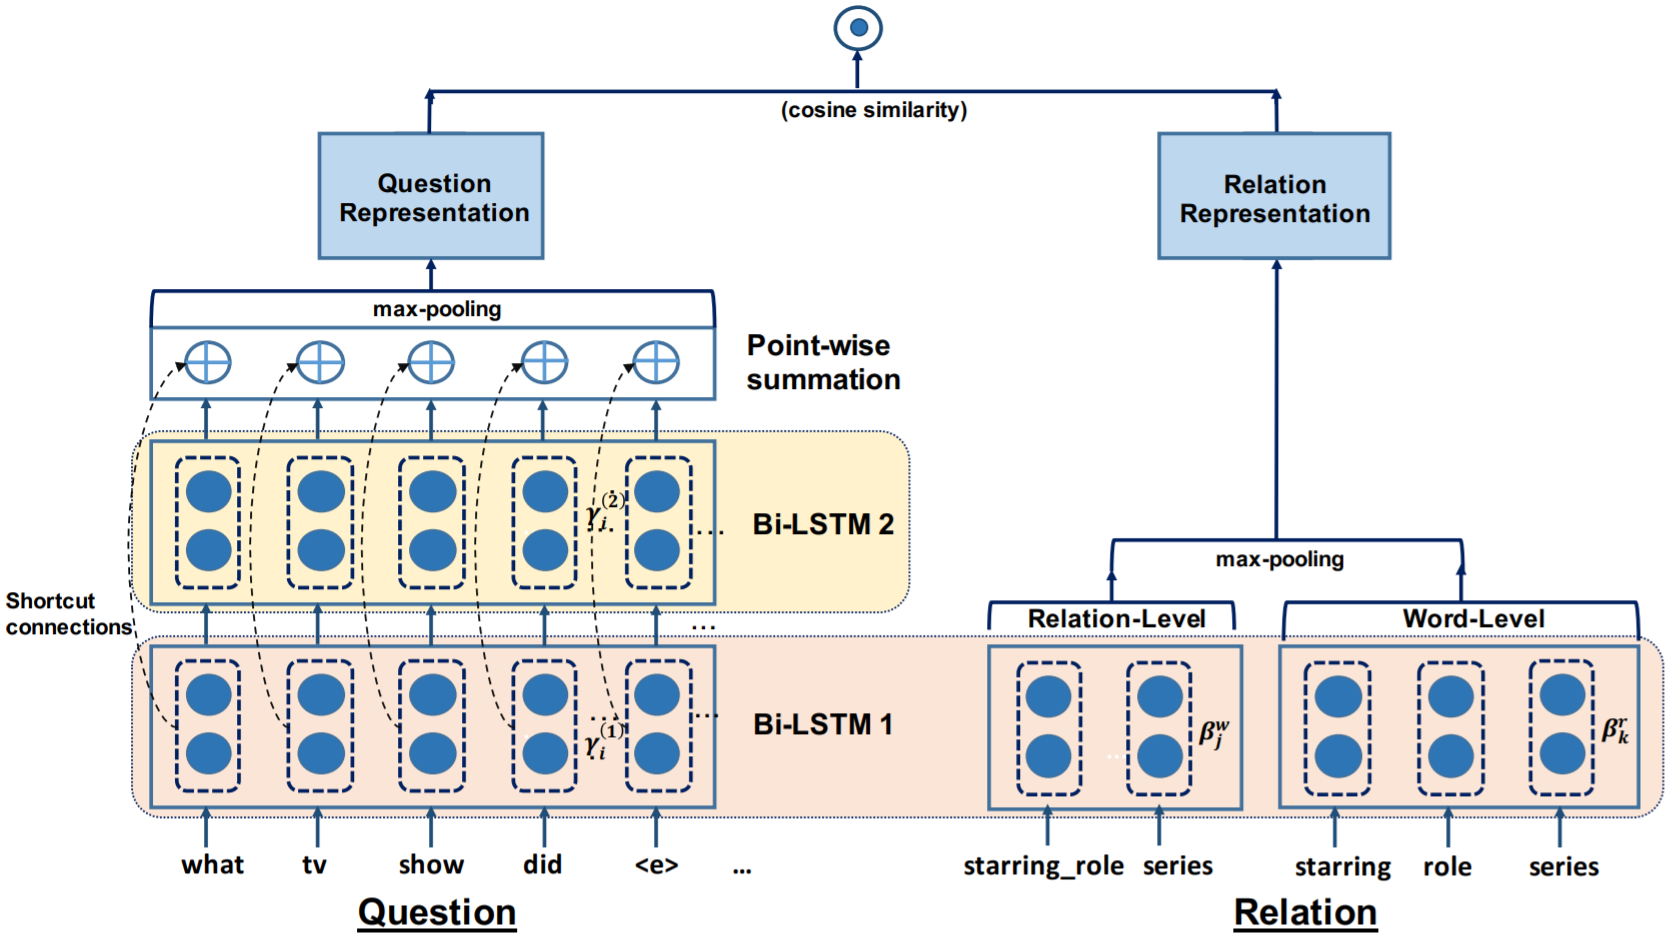
\includegraphics[width=0.95\columnwidth]{figure/rw/qa-hrbilstm.png}
\bicaption{HR-BiLSTM模型。\cite{yu2017improved}}{The HR-BiLSTM model.}
\label{fig:rw-siamese:a}
\end{figure}

对于WebQuestions等数据集上的复杂问题,如同\figref{fig:rw-spt:d}的查询图,
虽包含多条路径,但也可以选择其中最重要的路径作为主体与问句计算匹配程度。
微软的两个自动问答的研究工作\parencite{yih2015semantic,bao2016constraint}
利用了基于卷积神经网络的CDSSM匹配模型\cite{shen2014learning},
对问句和谓词路径的特征学习更多关注局部的词序信息,见\figref{fig:rw-siamese:b}。
其中,前一个研究工作由Yih等人\cite{yih2015semantic}提出,
深度学习模型仅关注问句和最重要谓词路径的匹配度,
对于查询图的其它分支路径,依然使用特征工程的方式寻找问句和谓词的字面匹配。
Bao等人\cite{bao2016constraint}的改进在于同样利用CDSSM模型,
对分支路径与问句中的特定上下文进行匹配,替代了繁琐的特征工程。
然而这些模型并没有能够学习到查询图整体在连续语义空间的特征表达,
不同路径的语义互相独立,因此面对复杂问题仍存在缺陷,这也是我们的研究重点。
%xu的先不聊
%找机会聊Hu和Cui,这两个最好还是提一提

\begin{figure}[ht]
\centering
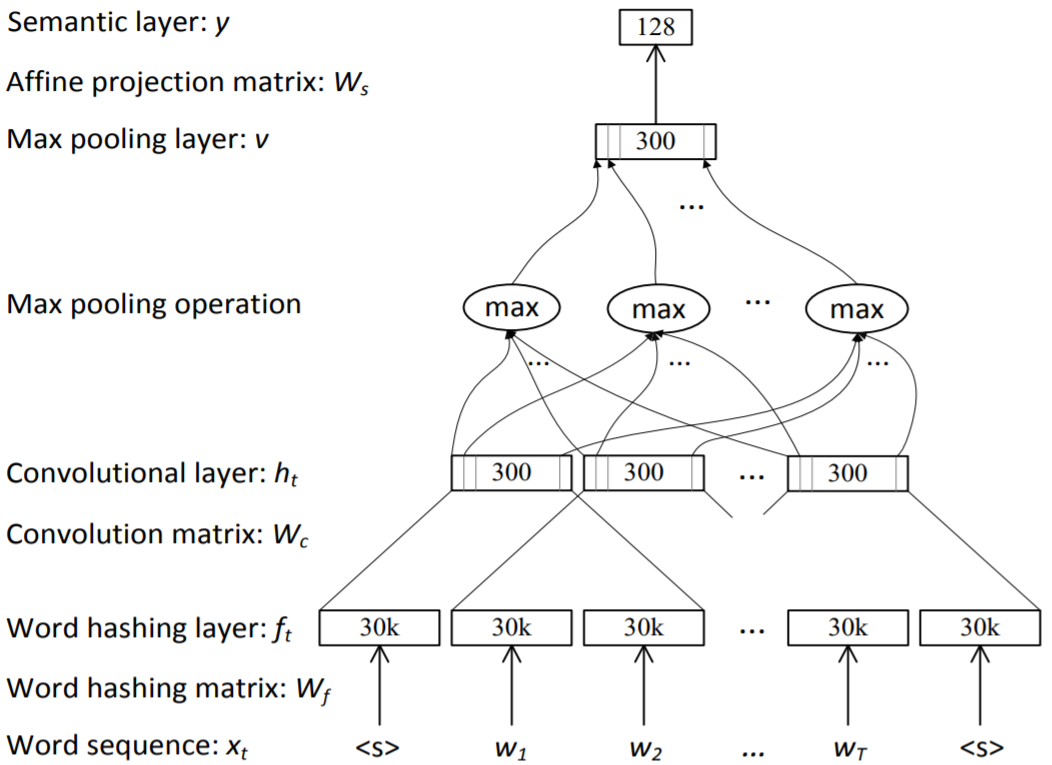
\includegraphics[width=0.6\columnwidth]{figure/rw/qa-cdssm.png}
\bicaption{CDSSM模型。\cite{shen2014learning}}{The CDSSM model.}
\label{fig:rw-siamese:b}
\end{figure}

%\begin{figure}[ht]
%  \centering
%  \subcaptionbox{HR-BiLSTM模型\cite{yu2017improved}\label{fig:rw-siamese:a}}
%    {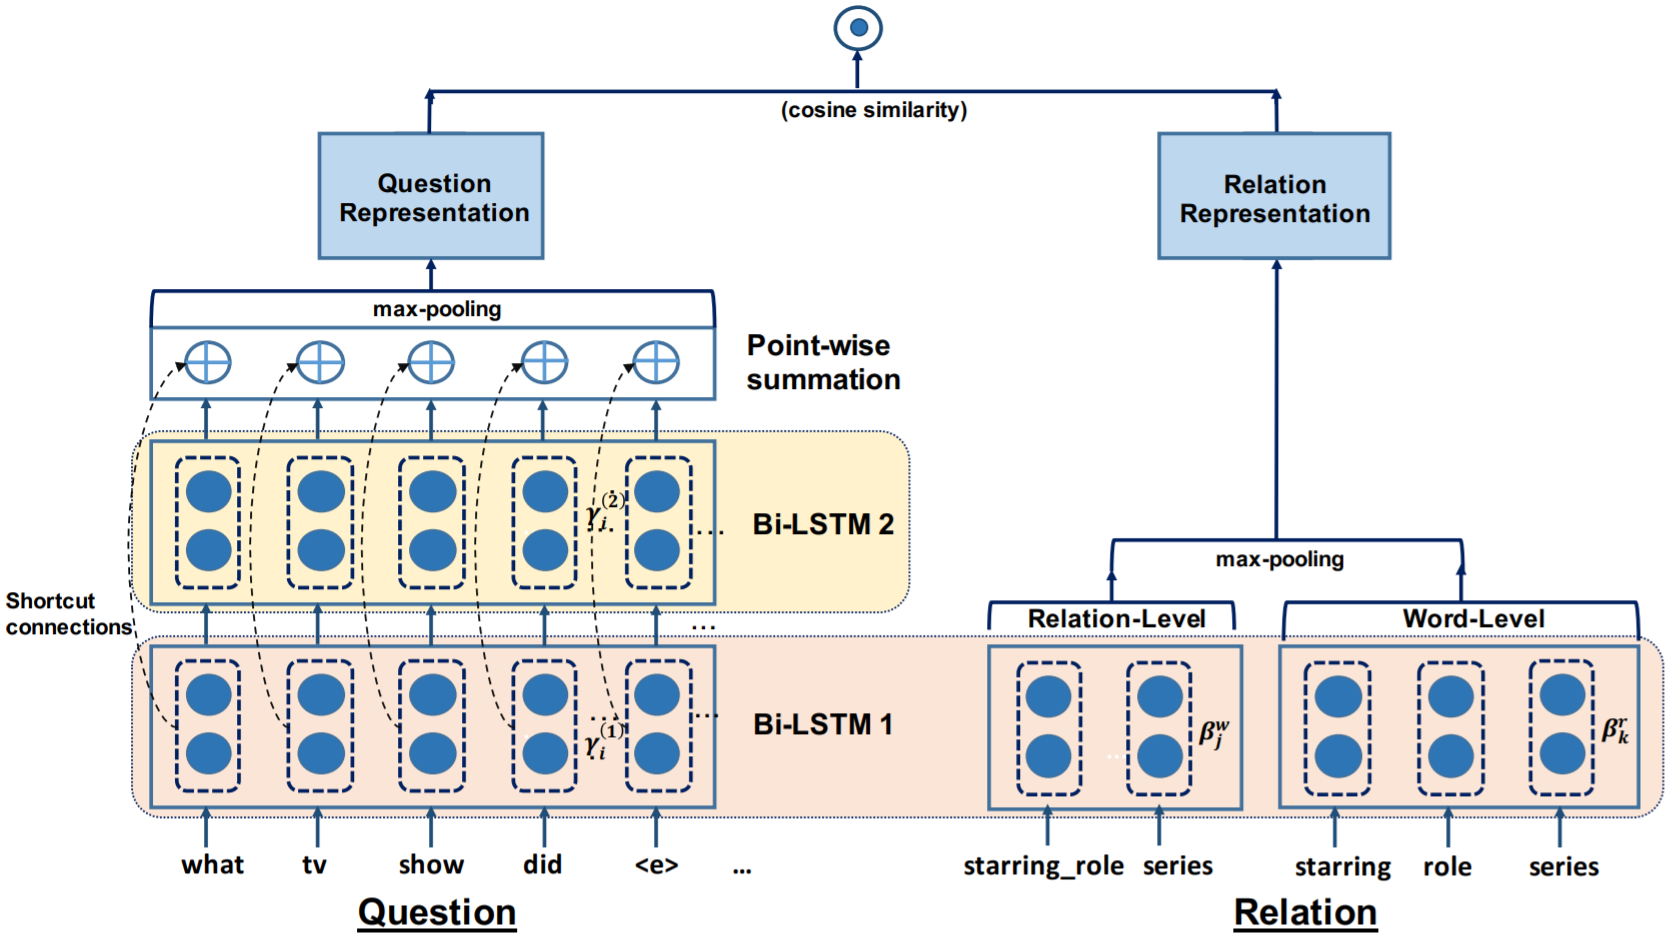
\includegraphics[width=0.48\columnwidth]{figure/rw/qa-hrbilstm.png}}
%  \hspace{1em}
%  \subcaptionbox{CDSSM模型\cite{shen2014learning}\label{fig:rw-siamese:b}}
%    {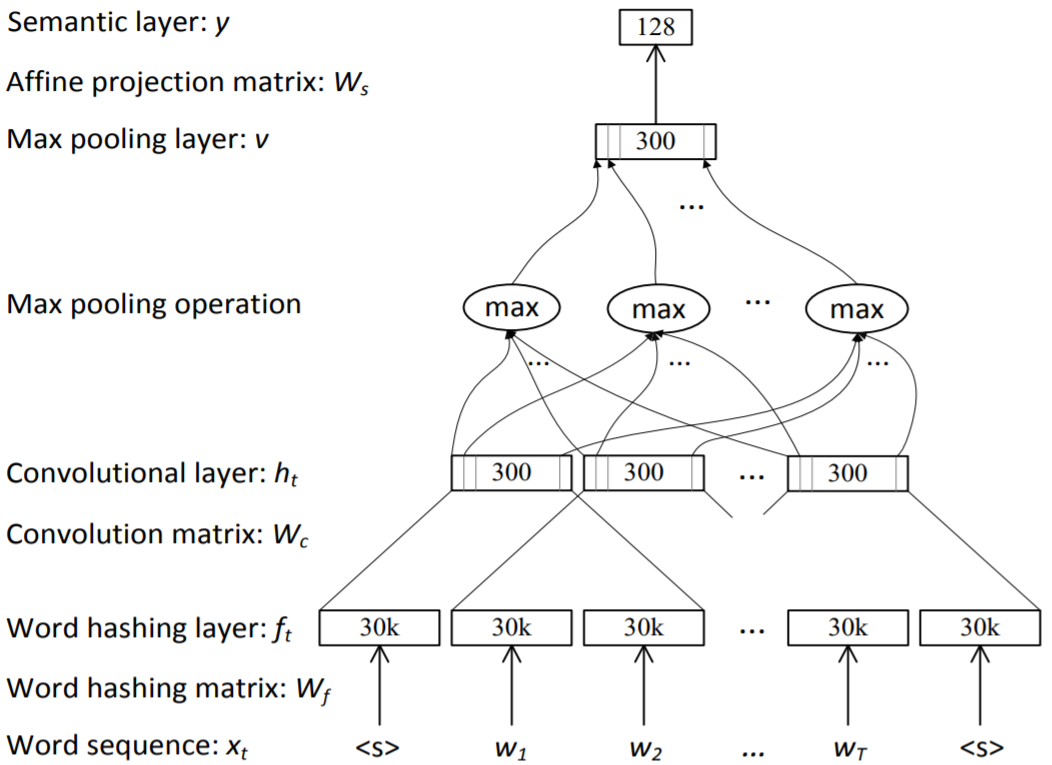
\includegraphics[width=0.48\columnwidth]{figure/rw/qa-cdssm.png}}
%
%  \bicaption{语义解析方法中,用于衡量语义匹配度的神经网络模型示例。}
%            {Example semantic matching models used in semantic parsing approaches.}
%  \label{fig:rw-siamese}
%\end{figure}

\subsubsection{训练方式}

训练方式的不同,主要取决于训练集中是否包含已标注的语义解析结构。
已有的问答数据集中,Free-917人工标注了每个问题的逻辑表达式,
QALD系列数据集则标注了SPARQL查询语句。
对于这些正确结构已给定的数据集,
可以直接利用监督学习算法进行匹配度训练。

显然语义结构的标注需要知识库领域的专家,因此标注过程会消耗大量人力,
更大规模的数据集例如WebQuestions和ComplexQuestions
仅包含每个问题的正确答案,而没有语义结构信息。
对于这些数据集,首先需要通过远距离监督方式构造可直接使用的训练数据,
即对所有训练问题,自动生成语义结构的正负样本。
已有的方法主要利用$F_1$分数衡量语义结构的好坏,
兼顾其生成的查询结果的准确率与召回率,即$F_1=2 \cdot P \cdot R / (P+R)$,
其中$P$代表准确率,$R$代表召回率。
再通过设定阈值将不同的语义结构划分为正负样本,
例如Berant等人\cite{berant2013semantic}仅将$F_1$分值为1(即答案完全匹配)
的语义结构作为正样本,
而Yih等人\cite{yih2015semantic}则将阈值设为0.5,
容忍一定程度的答案不完全匹配。
远距离监督方式避免了人工标注大量语义结构,
但考虑到语义偏差的存在,即答案正确的语义结构未必正确,
自动生成的训练数据也会引入一定量的错误。

%写类似p(g|q)之类的玩意儿刻画loss

%1. Template based (Bast, Yahya?)
%
%2. CCG (UBS, Kwai, CaiYates)
%
%3. DCS (Berant)
%
%4. Dependency Parsing Transform (Reddy, Hu)
%
%5. Staged Parsing (Yih, Bao)
%
%
%如何训练?
%
%传统Feature based (1,2,3)
%
%
%Improvements
%Berant14
%Yih
%Bao
%Xu...




\subsection{基于信息抽取的问答模型}

基于信息抽取的自动问答模型旨在直接从知识库中寻找正确答案,
而不尝试对问题进行具体化的语义建模。
模型主要包含三个步骤:
1) 对问句进行实体链接,得到其中包含的相关实体;
2) 在知识库中抽取出这些相关实体周围的其它实体,构成候选答案集合;
3) 计算问句与每一个候选答案的匹配度,以此预测出其中的正确答案实体。
显然模型的关键点在于第三步,即以怎样的特征描述候选答案与问句之间的关联。
在知识库中,一个实体所具有的信息主要包含它的名称、类型、
直接相连的谓词以及周围的其它实体。
这些信息组成了知识库中以该实体为中心的局部图,
不同的信息抽取模型都以这样的局部图作为候选答案实体的输入。
而这些模型的区别,在于特征的选取或学习方式。

Yao等人\cite{yao2014information}提出的模型利用特征工程方式,
将问句特征与候选答案特征进行配对组合,得到大规模的关联特征。
问句侧的特征来源于依存语法树,从中抽取出不同的依存路径,
以及具有强烈语义的词汇(如动词,wh-疑问词)。
答案侧的特征为答案的类型,以及与问句已知实体相连的谓词路径。
通过训练,具有高相关性的配对特征
(例如疑问词``where'' 与答案类型$location$配对)将具有更高的权重。

深度学习同样适用于基于信息抽取的问答模型。
Bordes等人\cite{bordes2014question}提出了QASE模型,
同样基于``{编码—比较}'' 框架,如\figref{fig:rw-ir:a}所示,
问句和候选答案的局部图分别进行编码,
问句的编码信息为每个词的出现次数,
候选答案则通过二进制编码表示答案实体自身、所属类型、相邻的谓词等信息。
模型学习映射矩阵$W$,将各自编码转换为连续空间上的语义向量,
$W$的每一行对应一个元素(词、实体、类型、谓词)的向量表示,
因此该模型实现了词向量和知识库向量的联合建模。

\begin{figure}[ht]
\centering
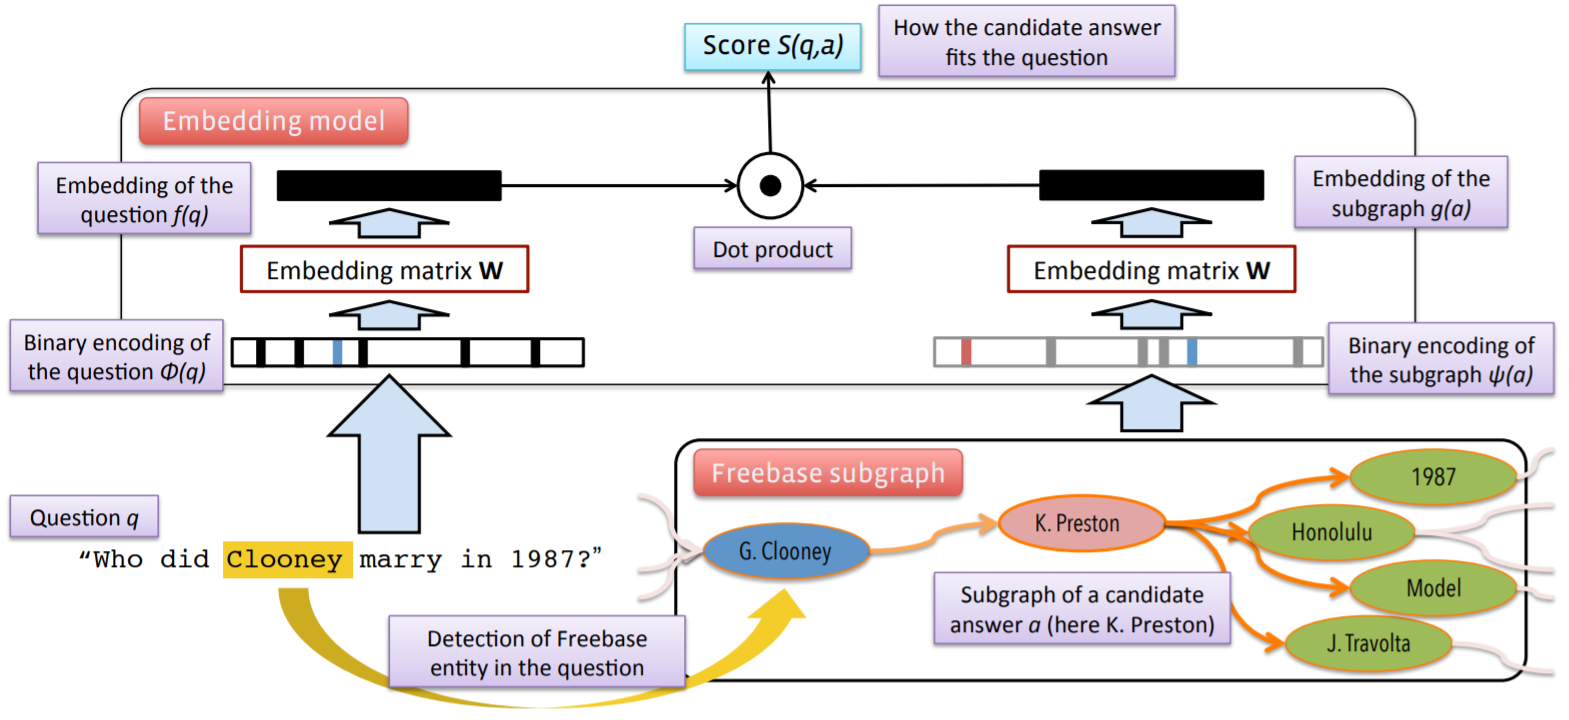
\includegraphics[width=0.95\columnwidth]{figure/rw/qa-qase.png}
\bicaption{QASE模型。\cite{bordes2014question}}{The QASE model.}
\label{fig:rw-ir:a}
\end{figure}

还有一些深度学习模型采用问句分别与答案相关的不同维度信息计算相似度,
再将各个维度的相似度进行聚合,得到问句与候选答案的整体匹配度。
Dong等人\cite{dong2015question}提出了MCCNN模型,
如\figref{fig:rw-ir:b}所示,
模型使用多个不同的卷积神经网络层对问句进行编码,
从而得到问句针对不同信息的向量表达。
将它们分别与答案的类型、谓词、上下文向量表达计算相似度之后,
最终的匹配度为这些相似度分值的总和,
使得模型在寻找最佳答案时能兼顾来自不同方面的匹配特征。

\begin{figure}[ht]
\centering
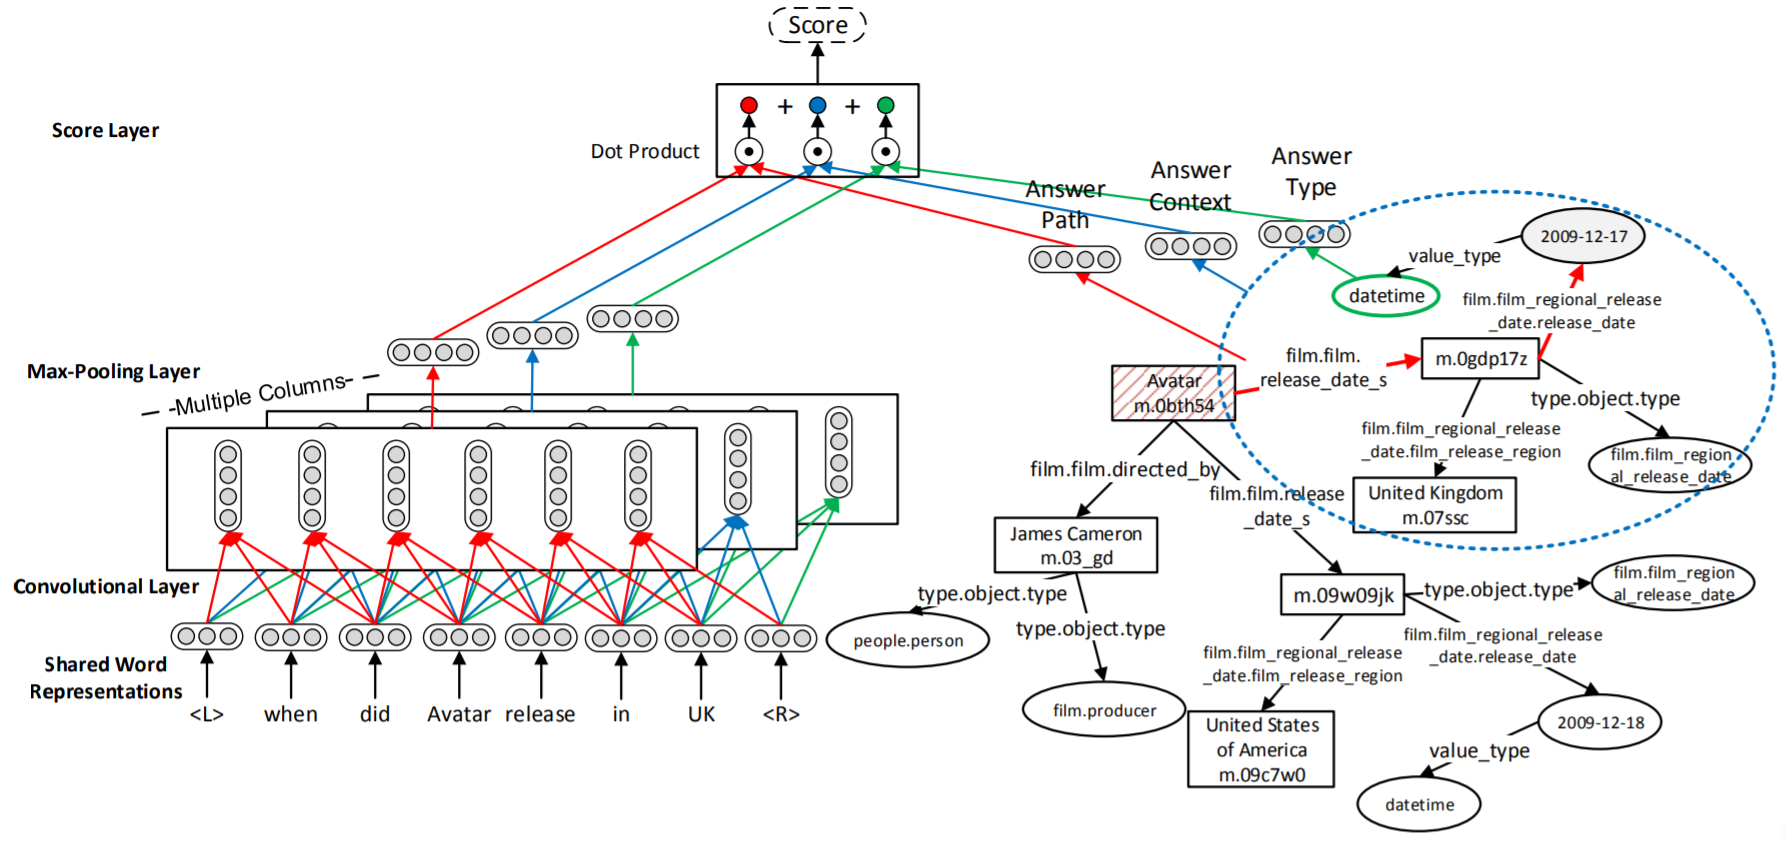
\includegraphics[width=0.95\columnwidth]{figure/rw/qa-mccnn.png}
\bicaption{MCCNN模型。\cite{dong2015question}}{The MCCNN model.}
\label{fig:rw-ir:b}
\end{figure}

Hao等人\cite{hao2017end}的模型在MCCNN基础上进行了改良,
除了将问句编码多个卷积层改为唯一一个双向LSTM层以外,
主要的贡献在于模型中使用了问句和答案之间的双向注意力机制。
一方面,针对答案在不同方面的表达,
答案对问句的注意力能够动态调整问句中不同词的重要性,
另一方面,问句对答案的注意力使得多个相似度分值互相之间也具有权重,
模型训练效果要优于无差别的求和操作。

%\begin{figure}[ht]
%  \centering
%  \subcaptionbox{QASE模型\cite{bordes2014question}\label{fig:rw-ir:a}}
%    {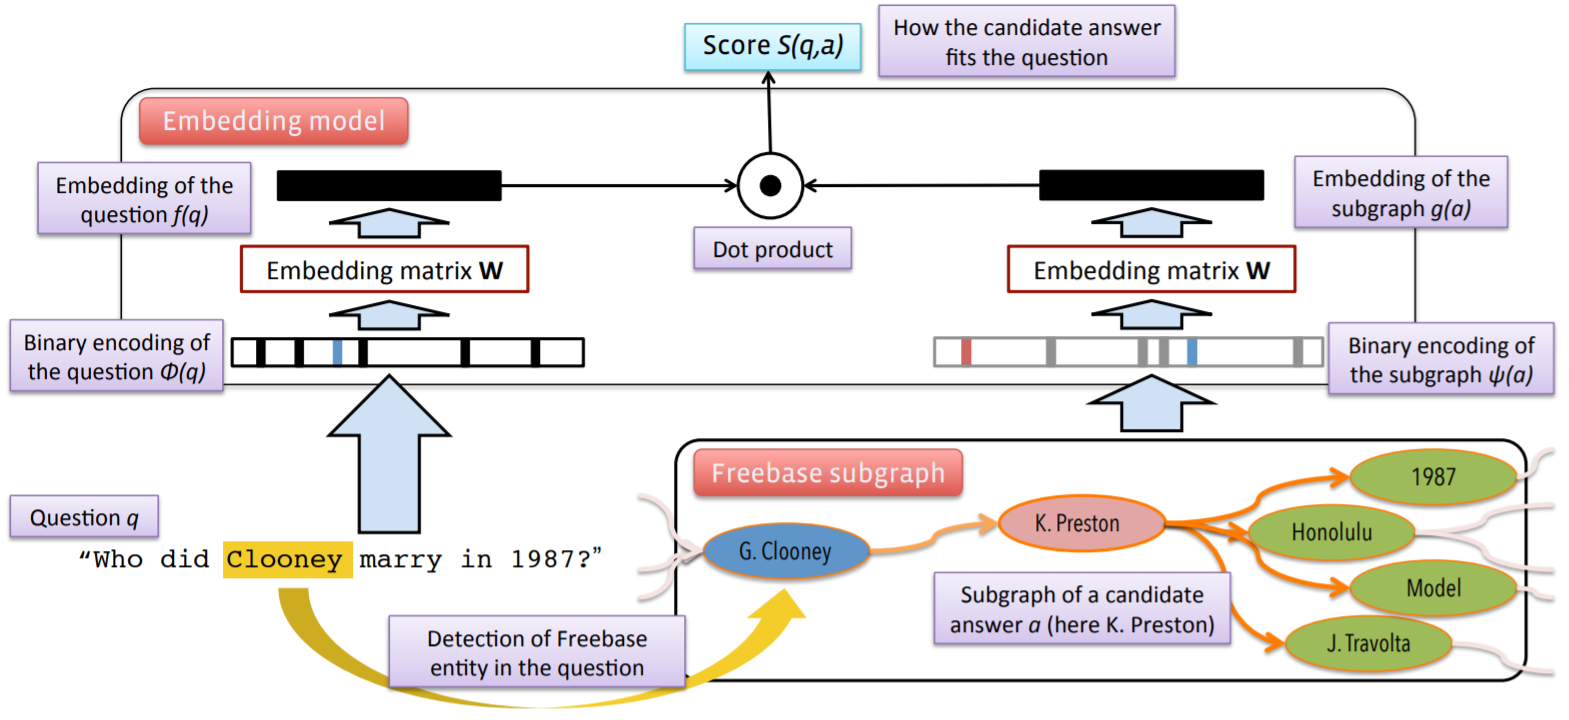
\includegraphics[width=0.48\columnwidth]{figure/rw/qa-qase.png}}
%  \hspace{1em}
%  \subcaptionbox{MCCNN模型\cite{dong2015question}\label{fig:rw-ir:b}}
%    {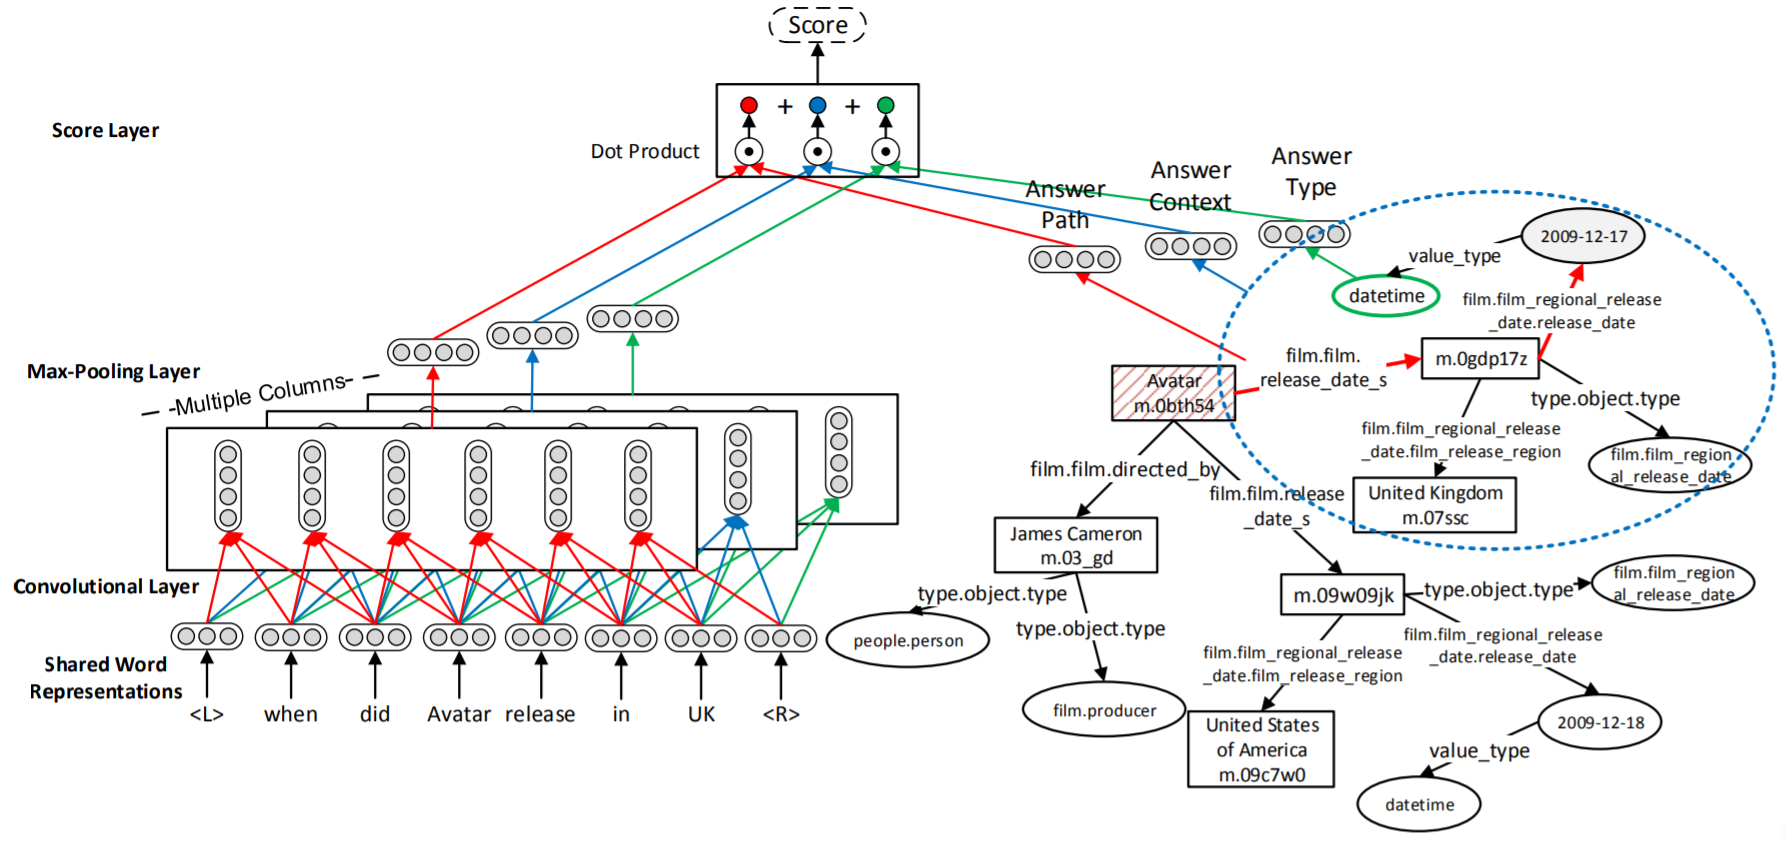
\includegraphics[width=0.48\columnwidth]{figure/rw/qa-mccnn.png}}
%
%  \bicaption{信息抽取方法中,用于衡量语义匹配度的神经网络模型示例。}
%            {Example semantic matching models used in information retrieval approaches.}
%  \label{fig:rw-ir}
%\end{figure}

和语义解析模型比较,
信息抽取模型实现了问答系统的端到端训练,
直接以\textless 问题,答案 \textgreater 作为训练数据,
防止远距离监督引入错误。
但同时也具有解释性较低的缺陷,
无法直接输出模型所理解的问句语义结构,
有时答案预测虽正确,但特征中可能存在语义偏差。
对于复杂语义的自动问答研究,
我们更在意语义结构的正确性,它能直接体现一个问答模型是否具有良好的语义理解能力。




\section{本章小结}
\label{chap:rw-summary}

本章对实体、关系、问句理解这三个层面的研究进行了背景介绍和文献综述。
实体理解方面,深度学习模型和跨语言词向量是我们较为关心的内容,
将会在第三章的跨语言表格链接任务中使用。
关系和问句理解方面,本章各介绍了两种路线不同的方法,
分别是关系理解的规则推导、知识库向量表示,
以及问句理解的语义解析、信息抽取。
这四种方法之间存在着一些共性:
规则推导和语义解析的共同点在于,
语义理解需要显式的语义结构(一阶逻辑表达式,或与之等价的知识库子图)作为媒介;
而另外两者的共同点在于对实体、类型、谓词等知识库元素进行表示学习,
以端到端的形式训练,模型更加面向具体任务。
在第四章和第五章的研究中,我们更加在意机器是否能理解具有复杂语义的关系或问句,
而不仅仅停留在特定任务的输出是否正确,
因此规则推导和语义解析是本文关注的重点。

%# -*- coding: utf-8-unix -*-
% !TEX program = xelatex
% !TEX root = ../thesis.tex
% !TEX encoding = UTF-8 Unicode


\chapter{跨语言的表格实体链接研究}
\label{chap:tabel}

本章研究的实体链接任务中,待链接文本为以源语言编写的互联网表格,
而知识库则以目标语言编写,因此我们将其称为跨语言的表格实体链接。
为了捕捉不同于传统实体链接任务的特性,
我们提出了基于神经网络和跨语言词向量的表格链接模型,
旨在让不同语言的连续特征空间得以兼容,并捕捉表格具有的多种粒度的匹配特征。
%在中英文跨语言表格链接实验中,本章提出的模型


%This paper studies the problem of linking string mentions from web tables in one language
%to the corresponding named entities in a knowledge base written in another language, 
%which we call the cross-lingual table linking task. 
%We present a joint statistical model to simultaneously link all mentions that appear in one table.
%The framework is based on neural networks, aiming to bridge the language gap by 
%vector space transformation and a coherence feature that captures the correlations 
%between entities in one table.
%%Experimental results show that our approach outperforms all baseline methods by a relative gain of 12.1\%,
%Experimental results report that our approach improves the accuracy of cross-lingual table linking
%by a relative gain of 12.1\%.
%Detailed analysis of our approach also shows a positive and important gain
%brought by the joint framework and coherence feature.~\footnote{Kenny Q. Zhu
%is the contact author. This work was supported by NSFC grant No. 
%91646205 and 61373031, as well as SJTU funding project 16JCCS08.}

%# -*- coding: utf-8-unix -*-
% !TEX program = xelatex
% !TEX root = ../thesis.tex
% !TEX encoding = UTF-8 Unicode

\section{概述}%intro
\label{sec:tabel-intro}

% basic introduction to table linking

海量的互联网文本信息中,充斥着以HTML编写的表格,
即互联网表格\cite{cafarella2008webtables,wang2012understanding}。
和纯文本相比,互联网表格中的行列形式携带了非常有价值的结构化信息。
为了能让机器理解,并且很好的处理表格中的信息,%~\parencite{wang2012understanding},
第一个步骤就是需要识别每个单元格中文本内容所对应的实体,
并映射到一个标准词库,或是知识库上,例如维基百科或Freebase。
这样的一个在互联网表格上进行实体链接的任务,
在本章节被称为表格链接\cite{bhagavatula2015tabel,wu2016entity}。

对于表格链接任务,
已有的研究工作\cite{bhagavatula2015tabel,limaye2010annotating}主要针对英文表格,
由于使用知识库也为英文,表格链接是在单一语言场景中进行的。
然而,当需要链接的表格以其它语言编写的时候,
对应语言的非英文知识库往往不够全面,无法涵盖目标表格中提及的所有实体。
例如中文版维基百科,其中包含的实体(页面)数量仅为英文维基百科的1/6左右。
%多聊几句?
基于不同语言知识库大小上的差异,
本章探寻一种全新的方式将非英文表格与英文知识库相连,
该任务也被称为\textbf{跨语言表格链接}。
如\figref{fig:tabel-intro}所示,
中文表格里的电影 ``{邮差}'' 在中文维基百科里没有对应的实体,
但存在对应的英文维基实体 ``Il Postino: The Postman'' ,
因此可以建立跨语言的链接。

\begin{figure}[th]
\centering
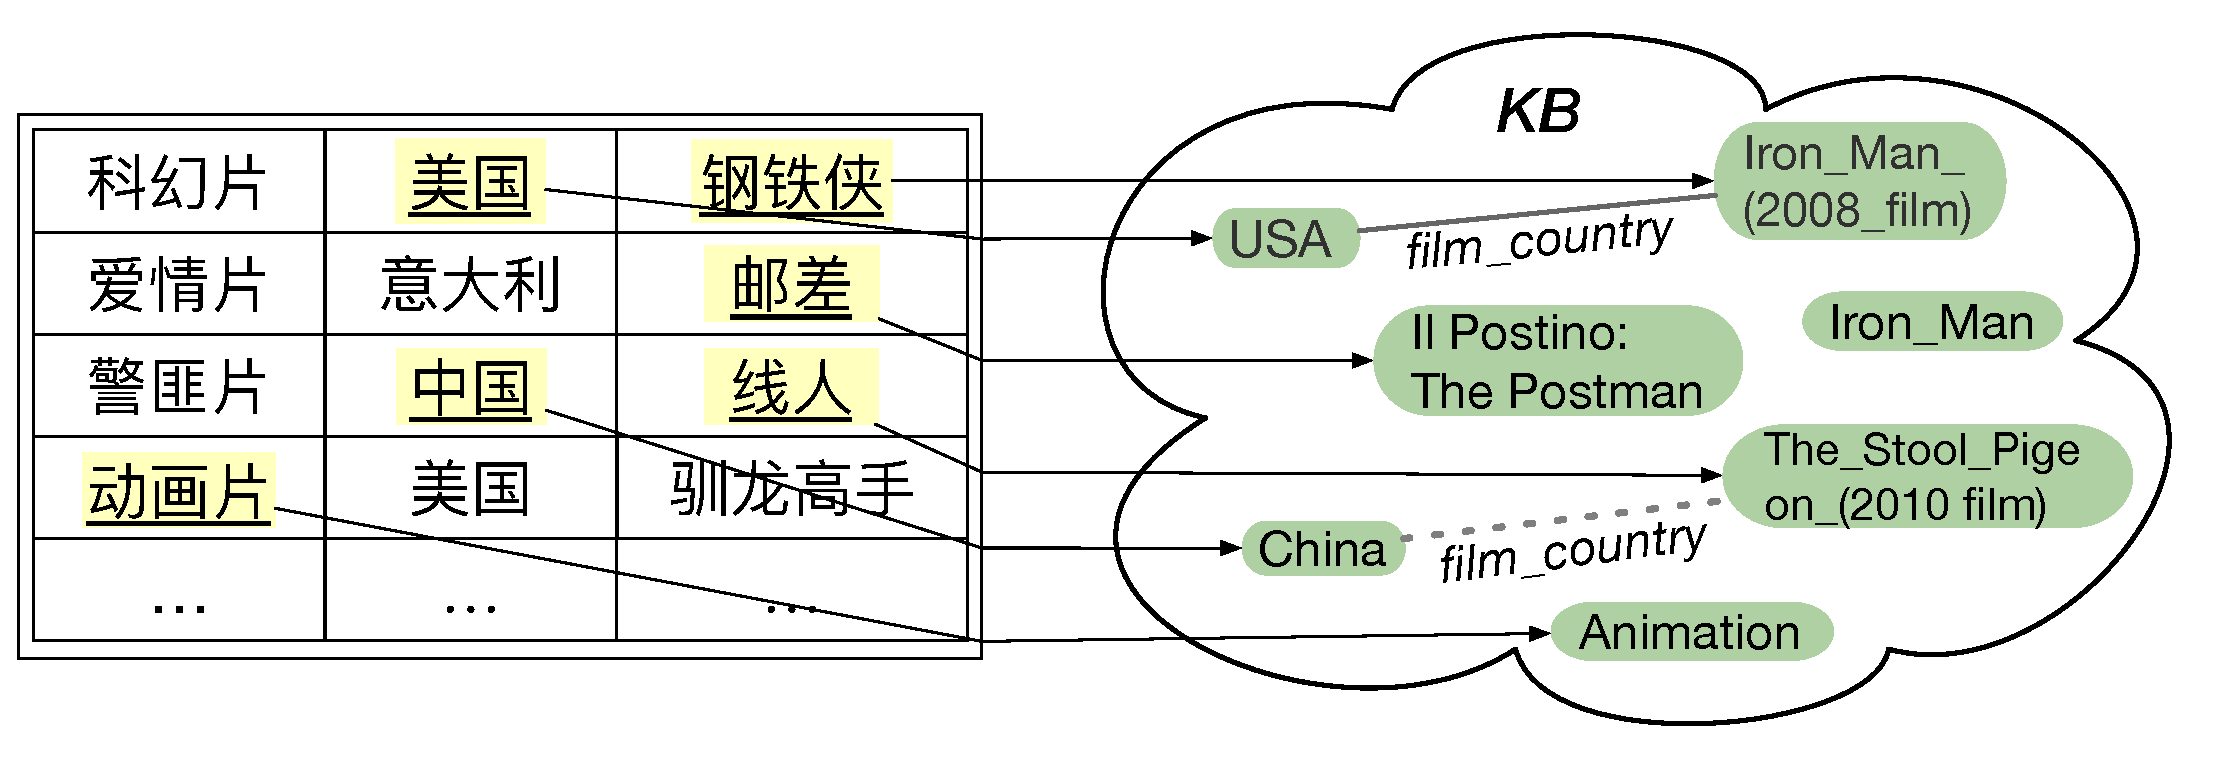
\includegraphics[width=0.9\columnwidth]{figure/tabel/intro.eps}
%\scalebox{0.22}{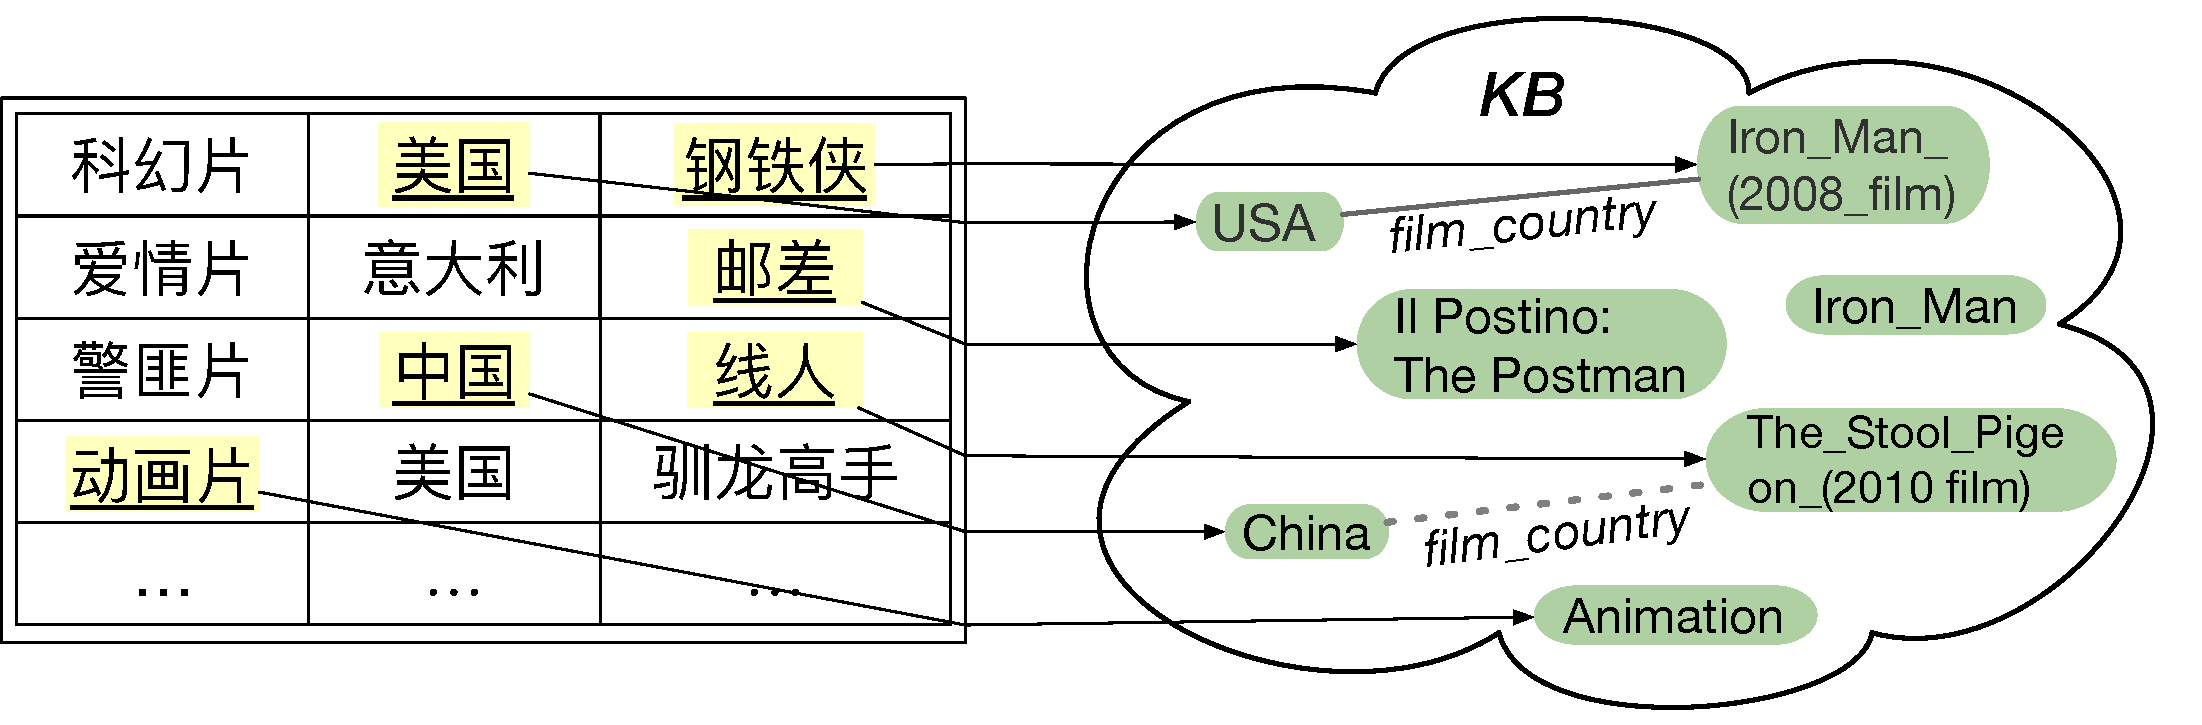
\includegraphics[angle=0]{figure/tabel/intro.pdf}}
\bicaption{中文表格到英文知识库的跨语言链接示例。}
{Example of cross-lingual table linking from Chinese to English.}
\label{fig:tabel-intro}
\end{figure}

帮助目标知识库补充事实三元组,是我们尝试跨语言表格链接的另一个动机。
英文知识库比其它语言知识库更加庞大,也更加结构化,但仍然包含许多长尾实体。
这些实体仅出现知识库的极少数事实三元组中,例如别国的电影、名人等,
考虑到英文知识库的贡献者更多以英语为母语,这些实体的相关信息就很容易被忽略。
另一方面,海量非英文的互联网表格成为了与长尾实体相关的丰富的语义信息来源。
例如,\figref{fig:tabel-intro}描述了电影与它的原产国之间的关系。
国产电影 ``{线人}'' 有对应的英文维基页面 ``The\_Stool\_Piegon\_(2010\_film)'' ,
但与之相应的Freebase实体却缺少许多相关的知识。
若我们准确将该电影链接至维基百科,
并根据表格前两列的多个实体对推理出关系$film\_country$,
那么就可为知识库补充新的事实。

%In this paper, we attempt to solve the cross-lingual table linking problem
%{\em without} using any non-English knowledge bases.
%%That is, our goal is to link the mentions in the non-English table 
%%directly to an entity in the English knowledge base. 
%%The advantage of this is we do not discard any information of non-English mentions
%%so that our model has the ability to tolerate the error caused by translation.
%To the best of our knowledge, this is the first attempt that attacks the 
%cross-lingual table linking problem. 


具体论述我们提出的跨语言表格链接方法之前,首先来讨论两种朴素的做法。
第一种方式主要基于已有单一语言的表格链接技术,
将表格映射到语言一致的非英文知识库,
然后再利用知识库之间存在的跨语言链接,%~\parencite{tsai2016cross},
将实体翻译至英文知识库。
例如不同语言的维基百科之间就存在着人工编辑好的跨语言链接。
这种方式的主要问题在于:
1) 非英文知识库的信息量较低,可能无法覆盖每一个单元格的实体;
2) 并不是每个非英文知识库都会存在和跨语言链接。

第二种做法中,整个非英文表格的内容首先直接被翻译成英文,
然后整个问题便退化成英文上的表格链接,以往方法可以直接套用。%\parencite{mcnamee2011cross}。
%这种两阶段方式依然不够有效,
它与远距离监督模型很相似,各单元格的(非英文名称,英文实体)对并不直接作为训练数据。
%翻译过程的错误会被传播到之后的链接步骤,而无法得到反馈。
此法的缺陷在于对已有翻译工具准确率的高度依赖:
一方面,文本翻译过程仅生成单一结果,一旦错误则对后续链接步骤影响很大;
另一方面,翻译工具如同黑盒,无法根据训练数据进行优化。

在本章中,为了使研究具有普适性,我们忽略不同语言知识库之间的跨语言链接,
尝试在\textbf{不使用}任何非英文知识库进行过渡的情况下,解决跨语言的表格链接任务。
据我们所知,本章节提出的解决方案,是对跨语言表格链接的第一次尝试。

对于实体链接任务而言,
%\parencite{tsai2016cross,mcnamee2011cross,bhagavatula2015tabel,wu2016entity},
无论是否跨语言,第一个步骤总是为每个单元格生成一组候选实体,
之后整个任务转换为排序问题,对每单元格寻找与其描述最接近的候选实体。
主要的技术挑战在于表格描述和知识库来自不同的语言,
无法依靠任何字面上的相似特征。
此外,表格中缺少纯文本里的谓语、状语等相关上下文,
给单个实体的消歧义带来了困难。
%The major technical challenge of our task is since the source mention
%and the target entity come from two different languages,
%their feature representations are naturally incompatible. 
%To make matters worse, tables offer very limited context for disambiguating
%a mention in the first place.

%Since the language of source mention and target entity is inconsistent, 
%it's hard to direct use the surrounding infomation of them \XS{rephrase}. 
%Besides, this task still has to face a lack of surrounding contexts 
%which can be very helpful during entity disambiguation in normal entity linking tasks.

% image CNN, table is like image

为了解决上述的两个挑战,
我们提出了基于神经网络的联合模型来解决跨语言表格链接问题,
它具有以下三个特点。
首先,模型主体基于跨语言词向量,我们将单元格的描述短语、%mention
上下文、以及知识库的实体映射到不同语言对应的连续向量空间作为语义特征表示,
并且使用线性变换的方式,实现不同语言的向量空间统一。
其次,模型充分利用表格中同一行列的实体所具有的相关性,
并通过神经网络学习不同粒度的相关性特征。
最后,模型基于联合训练思路,以优化整张表格的匹配程度作为目标函数,
使用成对排序损失函数进行参数学习以及多轮迭代的预测方式,对新的表格完成链接。

%Most existing work \XS{cite} mines hand-crafted features to measure the similarity 
%between mentions and candidate entities.  Since feature engineering suffers XXX, 
%some work attempt to use nerual network \XS{cite} to generate fearures, 
%which shows great improvements in task of entity linking. 
%
%As we should notice, a table can be regarded as a matrix of texts, similar to an image, which is a matrix of pixels. 
%Inspired by that idea of using deep neural networks to capture rich semantics of images, which has been proven successful, 
%we present a jointly modeling framework based on nerual networks to solve our problem.
%Besides, Convolotional Neural Networks(CNN) is a natural structure to deal with data in matrix form such as tables.

% Contribution
本章的贡献可以总结为以下四个部分:
\begin{enumerate}
\item{我们首次尝试在跨语言场景上进行表格链接;}
\item{我们提出了一个基于神经网络的联合训练模型,能有效捕捉原始表格与候选链接表格的语义相关性,
并消除不同语言之间的语义间隔;}%这一段写的很烂,可能要改
\item{联合模型除了捕捉单个单元格描述与候选实体间的语义关联特征,
还提出了一种一致性特征,用于捕捉候选链接表格内部不同实体间的联系,有效提升模型的预测准确率;}
\item{我们构建了从中文到英文的跨语言表格链接数据集用于实验,
本章提出的模型效果显著优于其它基线模型,
同时我们进行了一系列分析实验,以验证模型各部分的有效性。}
\end{enumerate}

%\begin{itemize}
%\item We are the first to define the problem of cross-lingual entity linking 
%for web tables (\secref{sec:problem});
%\item We present a novel neural network based joint model which effectively captures the rich semantics of mention table and referent entity table simultaneously. Based on that, we bridge the gap between different languages in this task (\secref{sec:translation} and \secref{sec:cell});
%\item We propose a coherence feature in the joint linking model which captures the correlation of entities appearing in the same table and improves the linking accuracy (\secref{sec:coherence});
%\item The framework significantly outperforms
%several baseline methods, with an accuracy of 62.9\%. (\secref{sec:eval}).
%%and question answering. Furthermore, our schema representation is
%%on par with the popular word embedding model in computing relation similarity (\secref{sec:eval}).
%\end{itemize}

%# -*- coding: utf-8-unix -*-
% !TEX program = xelatex
% !TEX root = ../thesis.tex
% !TEX encoding = UTF-8 Unicode

\section{相关工作}%related
\label{sec:tabel-related}

% %\label{sec:el}
% Entity linking has been a popular topic in NLP for a long time as it is the basic step for machines to understand natural language and an important procedure of many complex NLP applications such as information retrieval and question answering. Entity linking requires a knowledge base to which entity mentions can be linked, the most popular ones including Freebase~\cite{bollacker2008freebase}, YAGO~\cite{suchanek2007yago} and Wikipedia~\cite{cai2013wikification}, where each Wikipedia article is considered as an entity. 
% %Most works focus on linking to Wikipedia and thus the task is also named as Wikification. The typical procedure of entity linking contains two stages: candidate generation, where the surface forms (mention) in the query text which could be linked to certain entities in the KB are identified, and a set of candidate entities are proposed for each entity mention; candidate ranking, where the candidates for each mention are ranked (usually based on context) and the best one is returned as linking result. 
% Due to its fundamental role in many applications, the task of entity linking has attracted a lot of attention, and many shared tasks have been proposed to promote this study~\cite{ji2010overview,cano2014microposts2014,carmel2014erd}.
% %Wikipedia was first explored by Bunescu and Pasca~\cite{pasca2006using}, where an SVM kernel was used to compare the lexical context of an entity mention to each candidate's Wikipedia page. Since each entity mention needed to train its own SVM model, the experiment was limited. Later, Mihalcea and Csomai~\cite{mihalcea2007wikify!:} proposed a system called Wikify! for the Wikification task. They applied word sense disambiguation to this task, and experimented with two methods to link detected candidates to a Wikipedia page: 1) comparing the mention's lexical context to content of disambiguation page; 2) training a Naive Bayes classifier for each ambiguous mention. 
% %Later approaches made use of the observation that entity disambiguation in the same document should be related. Cucerzan~\cite{cucerzan2007large-scale} maximized the agreement between the context data stored for each candidate entity and the contextual information in the document, and also the agreement among the category tags of the candidate entities. Milne and Witten~\cite{milne2008learning} took a similar approach but relied on unambiguous terms in the context. Han and Zhao~\cite{han2009named} constructed a large-scale semantic network from Wikipedia, then computed similarity between query and candidate entity based on the semantic network. Ratinov et al.~\cite{ratinov2011local} formalized this task into a bipartite graph matching problem and proposed a score function which considered both local similarity and global coherence. Zhang et al.~\cite{zhang2011wikipedia} employed a Wikipedia-LDA model and the contexts were modeled as a probability distribution of Wikipedia categories. The similarity score between candidates and entities were computed based on the category distribution. 
% %Cai et al.~\cite{cai2013wikification} proposed to first enrich the sparsely-linked articles by adding more links iteratively and then use the resulting link co-occurrence matrix to disambiguate the mentions in an input document. Yang and Chang~\cite{yang2016s-mart:} proposed a tree-based structured learning framework, S-MART, which is particular suitable for short texts such as tweets. 
% 

对互联网表格的研究最早开始于Cafarella等人的工作\cite{cafarella2008webtables},
文中指出大约有1.54亿表格可以作为高质量的关系数据源。
例如文献\parencite{munoz2014using,sekhavat2014knowledge}关注于从表格中寻找
不同列之间的关系,从而实现向知识库中补充新的三元组。
这些工作都假定实体链接已完成,而若要对更广范围的表格数据进行关系挖掘,
表格链接始终是其前置步骤,链接准度直接决定了后续步骤的质量。
%如概述中指出,  表格关系可以补充三元组
%Munoz:找关系 挖掘不同行之间,但是是同样的两列之间的实体关系,映射至DBPedia 构成三元组,即挖掘语义。  并补充缺失
%在维基百科内部(已有链接)
%按已有match比例尝试一些predicate,然后学习一个triple是对还是错
%Sekhavat: Tabular KBC 同样是假设linking已好的情况 利用PATTY作为跳板,根据EP之间存在的pattern,寻找到rel的关系
%条件概率  (相当于EP有一系列的外部文本pattern,而不是仅有KB)
%rel来自YAGO
%(Fuck...但两者根本都是column-column-rel和predicate的一一对应)

和纯文本上的实体链接任务不同,表格文本上的链接聚焦于表格中的每一个单元格,
并且对于任何一个待链接的单元格,其它同行或同列的单元格与其有着更加密切的语义联系。
%不同的研究工如何利用好表格的半结构化
%如何利用同行列实体间的关联
目前已有的表格链接研究主要基于特征工程。
Limaye等人\cite{limaye2010annotating} 以YAGO为知识库,解决更加宽泛的表格链接任务,
包括将单元格链接至实体、列头链接至类型,以及两列之间的关系链接至谓词,
同时创建了WebManual数据集。
作者提出了一个概率图模型用于同时完成不同的链接子任务,
并通过人为定义的多种势函数表示单元格、实体、类型、谓词语间的组合特征,
整个表格链接的目标函数为多种势函数的连乘,不同子任务的决策互相影响,
使得模型在捕捉单个单元格与实体相匹配的同时,也能兼顾实体与列头类型的一致性,
以及不同列实体间与特定谓词的相关性。
%全局优化
%概率图模型,定义了potential,用于描述pair或这triple feature among type,entity,relation
%都是feature indicator
%1. cell vs entity (tfidf-cos, jaccard, soft-cos ...)
%2. header vs type (the same)
%3. entity vs type (e \in T)
%4. type vs rel (soft schema match)
%5. entity vs rel
%特征都比较直观简单,but,
%Experiments show that attacking the
%three subproblems collectively and in a unified graphical inference
%framework give clear accuracy benefits compared to
%making local decisions
Bhagavatula等人\cite{bhagavatula2015tabel}利用了表格上下文的词汇信息,
对于待链接的单元格,将其行或列方向上的其它单元格文本合并形成上下文词袋,
与候选实体所对应的词汇进行相似度计算,得到多个相似度特征用于模型训练,
并采用迭代更新方式进行预测。
%graph model,iterative update配上features
%每个cell确定了context之后独立计算
%上下文特征(word level,entity level)
%coherence(MW)
Wu等人\cite{wu2016entity}首次尝试对中文表格进行链接,
提出的模型首先构建由单元格和所有候选实体组成的连通图,
然后在图中进行类似PageRank算法\cite{page1999pagerank}
的随机游走,以选择最佳链接结果,因此是一种非监督学习方式。
候选实体是否同行列决定了图中是否存在直接相连的边,
而单元格与实体、实体与实体之间所连边的权重则由预定义的相似度公式计算,
使用了编辑距离、词袋相似度、实体于三元组中共现等特征。
区别与以上研究,本文的工作基于深度学习,尝试不依赖常用的相似度计算公式,
而是利用神经网络挖掘表格和目标实体在多个粒度上的特征。


% %\subsection{Cross-Lingual Entity Linking}
% %\label{sec:cl}
% Starting from 2011 the annual TAC KBP Entity Linking Track has been using the multi-language setting~\cite{ji2010overview,ji2014overview,ji2015overview}, where the languages involved are English, Chinese and Spanish. 
% %Most systems for this task were adaptations of mono-lingual entity linking systems: either first do entity linking on foreign languages and then translate the results to English via language links, which requires a comprehensive knowledge base in the foreign languages; or first translate the query into English by some machine translation tool and then apply English entity linking algorithms, whose performance greatly relies on the machine translator. 
% %Some other systems tried to avoid the usage of such assumptions. McNamee et al.~\cite{mcnamee2011cross} first experimented with cross-lingual entity linking on documents. They first used a machine translation tool developed by Irvine et al.~\cite{irvine2010transliterating} to transliterate the detected query mentions into English and transform the task into a mono-lingual one. Then they extracted some features and ranked the candidates with SVM-rank. However, to train this model, parallel corporas which are well aligned at sentence level are required.
% Most methods managed to bridge the language gap through language-independent spaces.
% Fahrni et al.~\shortcite{fahrni2011hits} presented HITS' system for cross-lingual entity linking. Their approach consisted of three steps: 1) obtain a language-independent concept-based representation for query documents; 2) disambiguate the entities using an SVM and a graph-based approach; 3) cluster the remaining mentions which were not assigned any KB entity in step 2.
% Zhang et al.~\shortcite{zhang2011wikipedia} leveraged a modified version of Latent Dirichlet Allocation, which they call BLDA (Bilingual LDA) and bridged the gap between languages via topic space. 
% %They trained the topic model on English-Chinese Wikipedia page pairs (indicated by inter-language links) and disambiguated candidate entities by computing the inner product of the topic distributions of the query text and the entity Wikipedia page. Their approach does not require supervised learning and performs well with a conservative candidate generation stage. 
% Wang et al.~\shortcite{wang2015language} proposed an unsupervised graph-based method which matches a knowledge graph with a graph constructed from mentions and the corresponding candidates of the query document.
% Tsai et al.~\shortcite{tsai2016cross} trained a multilingual word and title embeddings and ranked entity candidates using features based on these multilingual embeddings. 
% %They used canonical correlation analysis~\cite{hotelling1936relations} to project the embeddings of two languages into the same space, whose goal is the same as the translation layer in our model.


跨语言的实体链接的主要目的是将文本中的实体短语链接至另一个语言构建的知识库上,
近几年的TAC-KBP数据集\cite{ji2010overview,cano2014microposts2014,carmel2014erd}
中包含了跨语言的实体链接任务。
%以2015年的TAC-KBP任务为例,
%%Ji: Overview of the TAC-KBP2015 entity discovery and linking tasks 数据集
%目标知识库为英文维基百科,待链接的纯文本则来自英语、汉语、西班牙语这三种语言。
%相对于英文而言,其它语言下的知识库较为匮乏,
%因此跨语言实体链接的意义在于借助信息量更大的英文知识库,
%更好地理解外文文本中的信息。
为了解决此类问题,%跨语言场景中的实体链接任务,
McNamee等人\cite{mcnamee2011cross}提出了一种基线方法,
利用已有的翻译工具将外文文本转换为英语,
再使用传统的单语言链接模型完成任务。
%这样的方法,好处在于模型简单易于实现,
%但同时也具有一个很大的缺陷,就是
%此法的缺陷在于对已有翻译工具准确率的高度依赖:
%一方面,文本翻译过程仅生成单一结果,一旦错误则对后续链接步骤影响很大;
%另一方面,翻译工具如同黑盒,无法根据训练数据进行优化。
%TODO:后续如果有时间,可以聊聊cross-lingual word embedding,但肯定不是限制该干的事情。
为了尽可能减少对翻译工具的高度依赖,
模型需要能学习同一个实体或概念在不同语言下的抽象表达,
并通过特定运算体现出不同抽象表达之间的联系,以完成语义的跨语言兼容。

基于跨语言词向量的链接模型是一种可行的解决方案,
跨语言词向量的相关内容已在\secref{sec:rw-linking-cle}中介绍。
Tsai等人\cite{tsai2016cross}首先分别训练英文和外文的词向量,
再用典型相关分析(CCA)学习各自语言的转移矩阵,使得不同语言词向量位于同一连续空间,
之后依据该词向量计算短语和实体在不同粒度上下文中的余弦相似度,形成多个特征进行训练。
Sil等人\cite{sil2017neural}提出了更加复杂的深度学习模型,
以学习短语上下文和实体在句子级别和单词级别的相似特征,
同时在实验中比较了CCA、均方误差等多种生成跨语言词向量的方式。
%Sil 2016
%Wang
%fahrni
除了跨语言词向量以外,Zhang等人提出的跨语言主题模型\cite{zhang2013cross}
也可用于描述不同语言上的相同语义。
传统的LDA主题模型\cite{blei2003latent}旨在描述文档的语义表示,
通过对 ``{文档—主题}'' 与 ``{主题—单词}'' 间的概率进行建模,
将一个文档表示为抽象主题上的概率分布。
考虑到同一个实体在不同语言中的维基页面,
虽然单词不同,但其主题十分相似,
因此双语LDA模型中,同一个抽象主题对应不同语言上的两个``{主题-单词}'' 概率分布,
从而外语上下文和英语维基页面之间可以在主题层面上概率分布比较,实现链接过程。


本文的工作是表格链接和跨语言实体链接两者的综合体现,同时也是首次对此问题进行研究。

%# -*- coding: utf-8-unix -*-
% !TEX program = xelatex
% !TEX root = ../thesis.tex
% !TEX encoding = UTF-8 Unicode

\section{任务规范定义}
\label{sec:tabel-problem}

%The task of cross-lingual table linking: table info & entity info

%1. table info
%The task of cross-lingual table linking involves two kinds of information:
%mention tables and entities in the knowledge base.

输入的互联网表格$X$是一个具有$R$行和$C$列的矩阵,
每一个单元格$x_{ij}$的内容是由语言$L_1$(例如中文)描述的词语序列。
给定由另一种语言$L_2$(例如英文)编写,并包含大量实体$e$的知识库$K$,
跨语言表格链接的任务是寻找$X$对应的目标链接表格$E$,
使得链接表格中的每一个实体$e_{ij} \in K$对应单元格$x_{ij}$内容的消歧义表示。

在具体场景中,输入的表格包括一些无法被链接的单元格,
例如数字、日期、时间以及一些知识库中尚不存在的新兴实体。
一些已有工作\cite{ibrahim2016making}主要负责在互联网表格中识别这些数字或时间实体,
因此在本章中,我们不关注一个单元格是否能被链接的判断方式。
具体到任务定义中,
$P$为输入表格中所有可以被链接的单元格坐标$(i, j)$所构成的集合,
并且我们假设在训练集和测试集中,
每个输入表格$X$对应的可链接位置集合$P$都是已知的。

传统的实体链接方法通常在模型中定义一个评分函数$S(x, e)$,
用于衡量文本$x$与目标实体$e$之间的相关程度。
在表格链接任务中,这样的做法等同于将不同的单元格分割开,单独计算相似度。
然而缺陷在于,相邻或是同行列的目标实体之间的交互完全无法体现在链接模型中。
为了将目标链接表格中不同实体间的耦合关系融入任务中,
我们定义了在表格层面的评分函数,并以此预测最佳的链接表格$\hat{E}$,
如下所示:%TODO: argmax 显示错误
\begin{equation}
  \label{eqn:joint-score}
  \hat{E} = \argmax_{E \in GEN(X)} S(X,E),
\end{equation}
\noindent
其中$GEN(X)$表示由$X$生成的所有候选链接表格。
该函数描述了输入表格与候选实体表格之间的整体相关性分数。
%可以在这里扯joint和non-joint的区别。



%============================================================%

\section{我们的方法}
\label{sec:tabel-approach}

本节中,我们主要阐述使用联合训练模型解决跨语言表格链接的具体细节。
\figref{fig:tabel-overview}为整个模型的示意图。
之所以将整个模型成为 ``{联合训练模型}'' ,是因为神经网络的输入
包含了整个互联网表格$X$,以及对应的一个候选链接表格$E$,
而模型的输出代表两者的相关性分数$S(X, E)$。

具体而言:
1) 我们首先对表格中的每一个单元格内容生成一系列知识库中的候选实体;%(\secref{sec:candgen}),
2) 模型对单元格词组和实体进行向量编码,
并学习基于它们向量表示的\textbf{指示特征}以及\textbf{上下文特征};%(\secref{sec:cell}).
3) 为了使不同语言下的语义向量互相兼容,
模型利用双语翻译矩阵将向量表示从中文转为英文;%(\secref{sec:translation}).
4) 模型从候选表格$E$的内部学习第三类特征,即候选实体间的\textbf{一致性特征}。%(\secref{sec:coherence}).
%We combine these three features together to calculate the overall relevance score, and finally
本节最后将介绍训练和测试的具体流程,以及整个模型中重要的一些实现细节。%(\secref{sec:strategy}). 

\begin{figure*}
	\centering
	%\epsfig{file=figures/overview.eps, angle=0, width=2.0\columnwidth}
    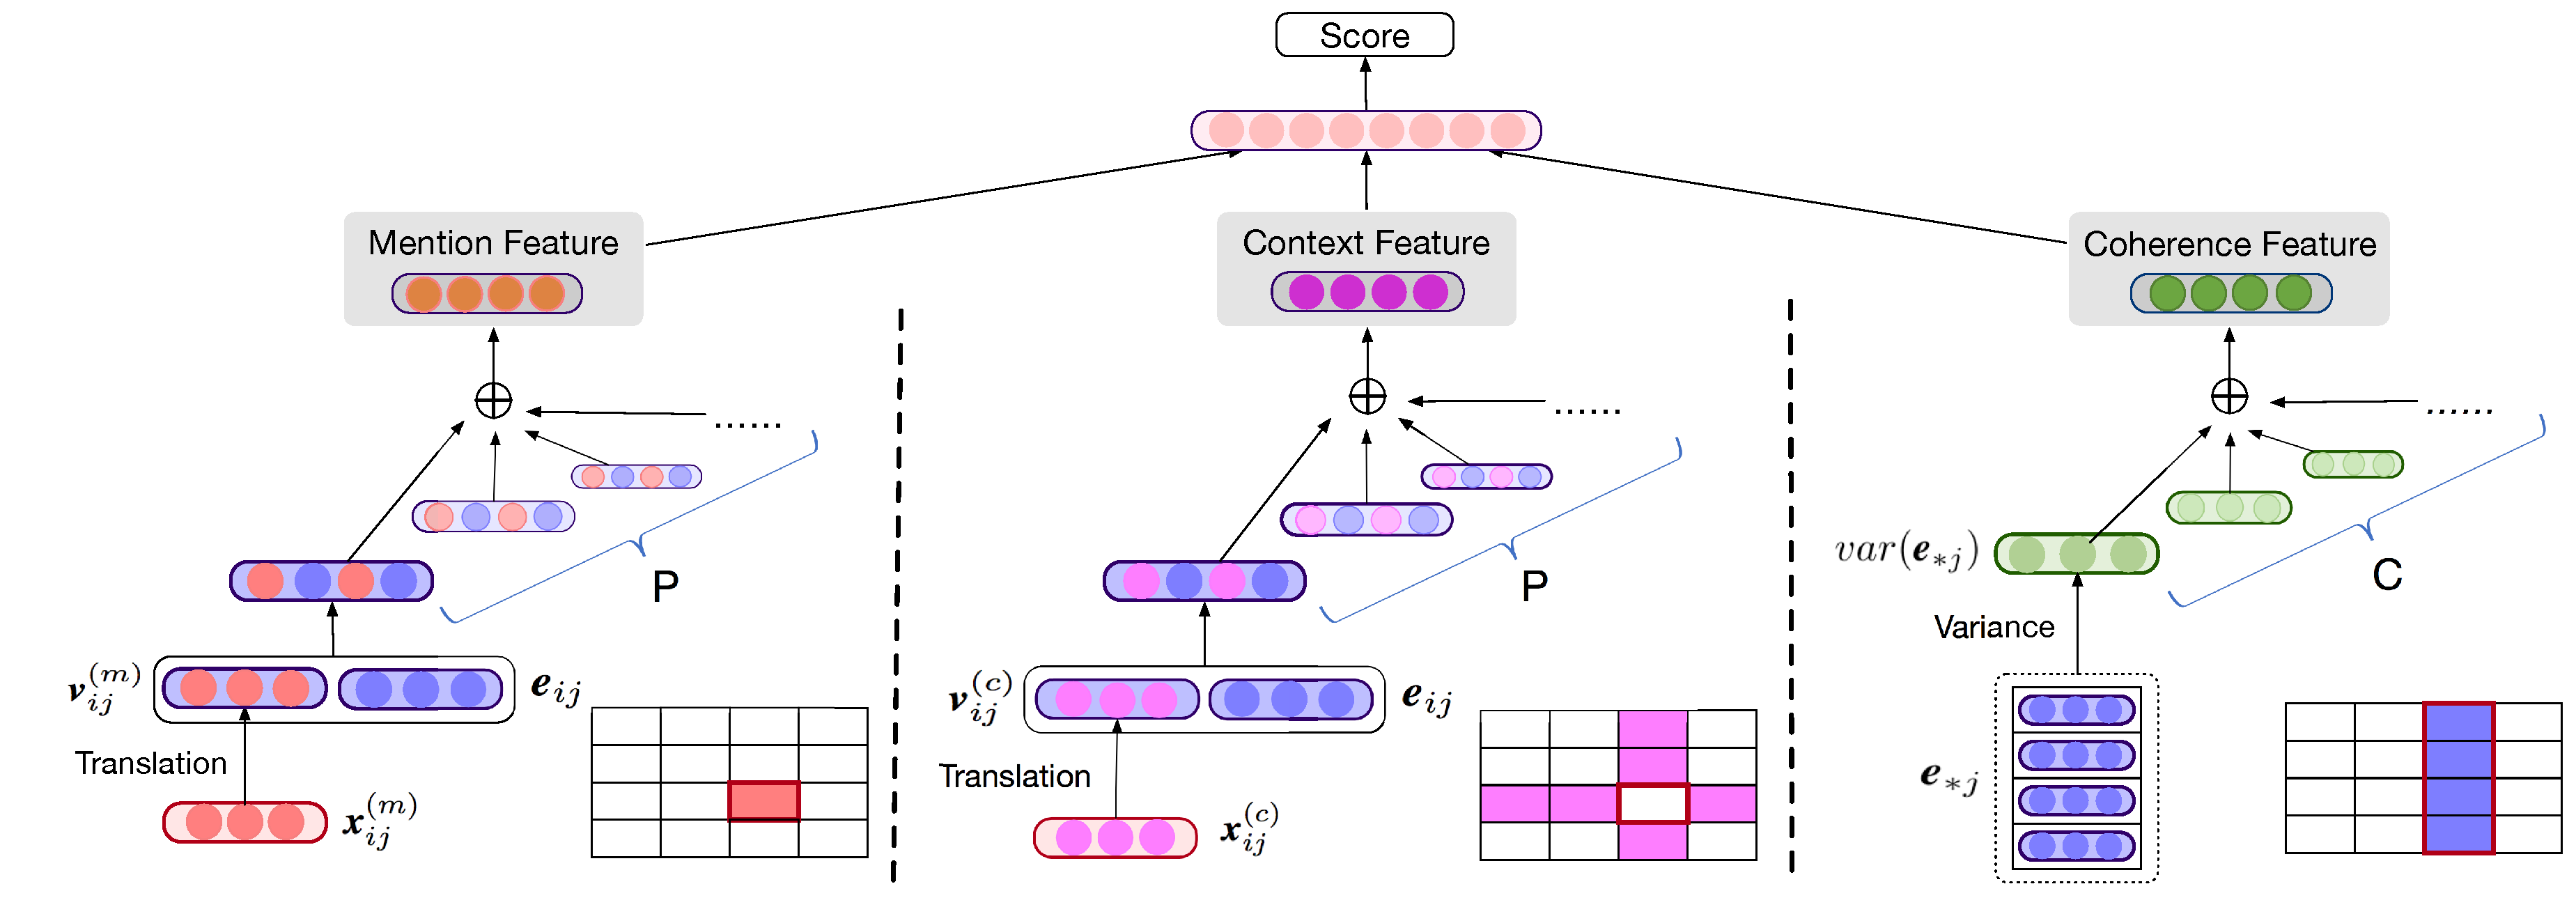
\includegraphics[width=\columnwidth]{figure/tabel/overview.eps}
	\bicaption{基于神经网络的联合训练模型示意图。}{Overview of proposed neural network based joint model.}
	\label{fig:tabel-overview}
\end{figure*}

%# -*- coding: utf-8-unix -*-
% !TEX program = xelatex
% !TEX root = ../thesis.tex
% !TEX encoding = UTF-8 Unicode

\subsection{候选实体生成}
\label{sec:tabel-candgen}

%To generate the candidate entity table,

我们对中文表格$X$的每一个单元格内容生成一系列英文知识库中的候选实体。
在本章的研究中,我们使用英文维基百科作为知识库。
由于提出的方法不使用任何中文知识库进行过渡,
为了实现语言转换,我们首先利用已有的翻译工具生成中文词组对应的多种翻译结果。
接下来,对于每一个翻译结果,我们都使用预先定义的启发式规则,将英文词组转换为候选实体。
这些实体的来源主要包括:
1) 名称与翻译完全匹配的实体;
2) 维基百科中,完全匹配的锚文本所指向的实体;
3) 通过计算编辑距离(Edit Distance)进行模糊匹配,并且相似度足够高的实体。
%可以具体讲一下细节
以中文词组 ``{疑犯追踪}'' 举例,不同的翻译工具生成的结果不同,
例如 ``person of interest'' 或者 ``suspect tracking'' 。
整体候选实体来自于每一个翻译结果的映射,例如维基百科中的实体
``person of interest'' , ``person of interest (tv series)'' 以及 ``suspect (1987 film)'' 。


%# -*- coding: utf-8-unix -*-
% !TEX program = xelatex
% !TEX root = ../thesis.tex
% !TEX encoding = UTF-8 Unicode

\subsection{向量表示及跨语言模块}
\label{sec:tabel-translation}

%字面描述=surface form
给定一个单元格的字面描述短语$x$,
令$\bi{x}^{(m)}$代表其自身的语义向量,也称为\textbf{指示向量}。
通常单元格字面描述较短(至多三个词语),
因此模型计算字面描述包含的词向量的平均,作为$\bi{x}^{(m)}$的值。
用$\bi{e}$表示候选实体$e$对应的实体向量,
词向量和实体向量分别通过中文和英文的维基百科文本进行预训练。

考虑到语言的天生差异,且两者分别训练,
因此词向量和实体向量所在维度空间并不兼容,
这使得我们无法简单地对来自不同空间的向量进行比较和计算。
为了应对这个问题,模型中引入了双语翻译层,将向量从一个语言的维度空间投影至另一个空间。
$\bi{x}^{(m)}$为中文语义空间上对$x$的语义表示,
该层通过线性变换将其映射为$\bi{v}^{(m)}$,即英文维度空间上的语义向量:
$\bi{v}^{(m)}=W_t \bi{x}^{(m)} + \bi{b}_t$。
其中$W_t$为变换矩阵,$\bi{b}_t$为偏置向量,两者均为模型参数,随着训练迭代而更新。
%为什么这么做,总要引用几篇论文吧

另外,我们通过少量的双语词对$(w^{(ch)}, w^{(en)})$,
对双语翻译层的参数$W_t, \bi{b}_t$进行预训练。
预训练过程的损失函数定义如下:
\begin{equation}
\label{eqn:translation}
L(W_{t}, \bi{b}_{t}) = \sum_i \Arrowvert W_{t} \bi{w}_i^{(ch)} + \bi{b}_{t} - \bi{w}_i^{(en)} \Arrowvert_2,
\end{equation}
即最小化真实的英文词向量与线性变换后的词向量之间的欧氏距离。
关于初始化,以及翻译预训练的更多细节,将在\secref{sec:tabel-impl}中进行叙述。


%As mentioned in model overview, the input of joint model are two tables, mention table and entity table, where each of them is represented as a table of vector embeddings. Since a mention or entity name typically contains up to three words, we simply represent them as the average of embeddings of words they contain. The word embeddings are trained on large scale text corpus. Since mention table and entity table are written in two different languages, we train word embeddings on two corpus of different languages separately. Thus, the embeddings of a mention and its referent entity are naturally incompatible and we can't directly compare or calculate them. To solve this problem, We employ a bilingual translation layer to map embeddings in one language space to another language space. Through this translation layer, a non-English mention embedding $v_m$ can be translated into an English mention embedding $\widetilde{v_{m}}$ roughly through $\widetilde{v_m} = W_{t} v_m + b_{t}$, where $W_{t}$ is the translation matrix and $b_{t}$ is the bias. Notice that $W_{t}$ and $b_{t}$ are model parameters and will be updated during training so that the translation step will be more and more accurate. \KZ{Do we need to entity link the english corpus to train the embedding?
%Since the entity table contains the entities and not names?}
%
%In order to find a good starting point to train the model and jump out of local optima, we train $W_{t}$ and $b_{t}$ in advance. We use a small number of bilingual word embedding pairs $\langle v_{wc}, v_{we} \rangle$ to train the parameters. The loss function is as follows.
%\begin{equation}
%\label{eqn:translation}
%L(W_{t}, b_{t}) = \Arrowvert W_{t} v_{wc} + b_{t} - v_{we} \Arrowvert_2
%\end{equation}
%The list of bilingual word embedding pairs are called translation seeds. We learn a initial translation matrix by minimize the loss and then feed the weights into the model before training.
%\KZ{So this is just to obtain the initial values for $W_t$ and $b_t$ 
%to be trained in the main training process?  How do you obtain the seed pairs?}




\subsection{指示特征与上下文特征}
\label{sec:cell}

如\figref{fig:tabel-overview}所示,最左边的部分对应指示特征模块,
中间的部分对应上下文特征模块。
两者的共同点在于,它们都关注互联网表格$X$与候选链接表格$E$之间的相似性或相关性,
并且每个单元格各自计算的特征会聚合为一体。
因此这两部分具有很相似的网络结构。

首先介绍指示特征,它捕捉一个单元格自身描述与目标实体的对应。
给定字面描述$x_{ij}$,
我们将英文的指示向量$\bi{v}_{ij}^{(m)}$与实体向量$\bi{e}_{ij}$进行拼接,并送入全连接层,
生成单元格在自身指示级别的隐含特征。%~\parencite{socher2013reasoning,socher2013recursive}。
%we concatenate the translated embedding $\bi{v}_{ij}^{(m)}$ with the entity embedding $\bi{e}_{ij}$~\parencite{socher2013reasoning,socher2013recursive},
%then feed into a fully connected layer,
%obtaining the hidden feature between $x_{ij}$ and $e_{ij}$ at mention level.
收集所有需要被链接的单元格的指示特征,并对其求平均,
即可得到整张表格上的总体指示特征$\bi{h}^{(m)}$。
具体公式如下:
\begin{equation}
  \label{eqn:tabel-mention}
  \begin{aligned}
    & \bi{f}_{ij}^{(m)} & = & \bi{g}(W^{(m)} [\bi{v}_{ij}^{(m)}; \bi{e}_{ij}] + \bi{b}^{(m)}) \\
    & \bi{h}^{(m)}      & = & \frac{1}{|P|} \sum_{(i,j) \in P} \bi{f}_{ij}^{(m)},
  \end{aligned}
\end{equation}
\noindent
其中$W^{(m)}$以及$\bi{b}^{(m)}$为模型参数,
$\bi{g}$为非线性激活函数,实验中使用ReLU函数。

%As shown in \figref{fig:overview}, the output of our model is a score, which represents the linking confidence between a mention table and a candidate entity table. This score comes from two categories. One is to measure how similar or compatible two tables are. We employ two features called cell feature and context feature to capture the compatibility between mention table and candidate entity table.
%
%After translation layer, each mention embedding $v_{\textbf{m}_{ij}}$ is converted into the same vector space as entity embedding. We concatenate translated mention embedding $\widetilde{v_{\textbf{m}_{ij}}}$ with entity embedding $v_{\textbf{e}_{ij}}$ and then go through a fully connected layer to get a hidden feature for a pair of cells $\langle \textbf{m}_{ij}, \textbf{e}_{ij}\rangle$. After averaging among all cells which need to be linked, we get the cell feature, which now represents a pair of tables $\langle T_M, T_E \rangle$.
%
%\begin{equation}
%f_{cell}(T_M, T_E) = \frac{1}{|P|}\sum_{\langle i,j\rangle \in P}FC([\widetilde{v_{\textbf{m}_{ij}}}, v_{\textbf{e}_{ij}}])
%\end{equation}
%
%Where $FC$ represents fully connected layer, and $[v_1, v_2]$ means vector concatenation.

上下文特征的获取与指示特征类似。
区别于指示特征的信息仅来自目标单元格,
上下文特征还将考虑此单元格周围的有用信息。
而在表格之中,位于同一行或同一列的其余单元格则具有直接的关联,
因此成为上下文特征的信息来源。
我们定义一个单元格的上下文向量$\bi{x}_{ij}^{(c)}$
为这些相关单元格指示向量的平均:
\begin{equation}
%  \begin{gathered}
    \bi{x}_{ij}^{(c)} = \frac{1}{|R+C-1|}(
      \sum_{(i,k), k \neq j} \bi{x}_{ik}^{(m)} +
      \sum_{(k,j), k \neq i} \bi{x}_{kj}^{(m)}
    ).
%    \bi{v}_{ij}^{(c)} = W_t \bi{x}_{ij}^{(c)} + \bi{b}_t.
%  \end{gathered}
\end{equation}
\noindent
同样经过双语翻译层的转换,英文空间中每个单元格的上下文向量$\bi{v}_{ij}^{(c)}$
将用于生成整个表格的总体上下文特征,记做$\bi{h}^{(c)}$。
具体计算过程类似\eqnref{eqn:tabel-mention},
只需要把所有指示向量改为上下文向量作为输入即可。
通过观察表格中的每个\textless 字面描述,候选实体 \textgreater 对,
并进行指示特征和上下文特征的学习,
模型可以从两张表中捕捉大体上的语义相关程度。

%\begin{equation}
% \begin{aligned}
%   & \bi{v}_{ij}^{(c)} & = & \frac{1}{|R+C-1|}(
%     \sum_{(i,k), k \neq j} \bi{v}_{ik}^{(m)} +
%     \sum_{(k,j), k \neq i} \bi{v}_{kj}^{(m)}
%   ) \\
%   & \bi{f}_{ij}^{(c)} & = & relu(W^{(c)} [\bi{v}_{ij}^{(c)}; \bi{e}_{ij}] + \bi{b}^{(c)}) \\
%   & \bi{h}^{(c)}      & = & \frac{1}{|P|} \sum_{(i,j) \in P} \bi{f}_{ij}^{(c)},
% \end{aligned}
%\end{equation}
%
%\begin{equation}
%	f_{cxt}(T_M, T_E) = \frac{1}{|P|}\sum_{\langle i,j\rangle \in P}FC([\widetilde{vcxt_{\textbf{m}_{ij}}}, v_{\textbf{e}_{ij}}])
%\end{equation}
%
%\begin{equation}
%vcxt_{\textbf{m}_{ij}} = \frac{1}{|\pi_{ij}|}(\sum_{\langle i,k\rangle \in P, k \neq j} v_{\textbf{m}_{ik}} + \sum_{\langle k,j\rangle \in P, k \neq i} v_{\textbf{m}_{kj}})
%\end{equation}
%\noindent
%where $\bi{h}^{(c)}$ denotes the hidden context feature of the mention-entity table pair.
%Despite that table offers rare ``strict'' context information for entity disambiguation,
%mentions in the same row or column contain strong relatedness and can be regarded as surrounding context. 
%By learning cell feature and context feature from mention table and candidate entity table,
%we can capture a general sense of semantic relatedness of all mention-entity pairs from two tables.



\subsection{一致性特征}
\label{sec:tabel-coherence}


前面叙述的两类特征都是对互联网表格与链接表格之间的契合度进行编码,
另一方面,链接表格内部,不同实体之间的关系同样具有价值。
之所以有这样的理解,是因为表格中同一列(有时同一行)的实体大多都属于同一种类型,
也就是说,往往拥有更加相似的向量表达。
例如概述部分的\figref{fig:tabel-intro},表格中从左到右三列,
对应的链接实体分别属于电影流派、国家、电影。
我们提出的第三种特征,正是用来描述同一列候选实体之间的契合度。

%\KZ{How do you distinguish between columns and rows?  Some tables have same-type columns, while others have same-type rows.}
%\XS{Cite papers doing table type classification, where one of those table types (6 in total) is called Vertical Relational (VR), which is exactly the format of tables in our experiments. We could say we just choose to focous this type of tables, and one can use those classifiers to unify table formats into VR and then use our model to do entity linking. }

关于同一类型的实体在表格中是按哪种方向进行排列,
这涉及到另一个研究课题名为 ``{表格类型分类}''
\cite{eberius2015building,nishida2017understanding},
主要用于区分表格的多种表现形式。
本章中默认表格的形式为 ``{垂直关系型}'' \cite{nishida2017understanding},
即和\figref{fig:tabel-intro}一样,相同类型实体按列方向排布。
考虑到确定表格类型之后,大多数互联网表格都可以实现简单的格式转换,
因此这个课题不在我们的讨论范围。

一致性特征的网络结构见\figref{fig:tabel-overview}的最右侧部分,
为了衡量一列实体向量是否接近,
我们对这些向量进行逐位的方差计算,方差越小,
表明这些实体在对应位置的隐含语义上差别越小,反之亦然。
同样对每一列的方差向量进行求平均的操作,
我们便得到整个候选实体表格上的一致性特征$\bi{h}^{(coh)}$:
\begin{equation}
  \label{eqn:coherence}
    \bi{h}^{(coh)} = \frac{1}{C} \sum_{j} \bi{var}(\{\bi{e}_{ij} | (i,j) \in P \}),
\end{equation}
\noindent
其中$\bi{var}(\cdot)$函数以向量集合作为输入,返回同样维度的逐位方差向量。
一致性特征用于描述候选实体互相之间是否有良好的自我组织性,
由于和字面描述表格$X$无关联,
该特征可以看做对指示特征与上下文特征的补充。


\subsection{训练及测试}
\label{sec:tabel-strategy}

%表格链接任务被定义为计算输入互联网表格与链接表格间的
我们首先定义输入表格$X$与候选链接表格$E$之间的整体相关性分数。
前面提及的指示、上下文、一致性特征将被拼接,并送至一个两层的全连接网络得到总体特征$\bi{h}_{out}$,
第二层的输出维度为1,即表示最终的表格相关度:
\begin{equation}
  \label{eqn:score}
  \begin{gathered}
    \bi{h}_{out}  = \bi{g}(W_{out}[\bi{h}^{(m)}; \bi{h}^{(c)}; \bi{h}^{(coh)}] + \bi{b}_{out}) \\
    S(X, E)         = \bi{u} \cdot \bi{h}_{out},
%score(T_M, T_E) = W_{out} \cdot FC([f_{cell}, f_{cxt}, f_{coh}]) + b_{out}
  \end{gathered}
\end{equation}
\noindent
其中$W_{out}$,$\bi{b}_{out}$以及$\bi{u}$均为模型参数。
%$\bi{g}$为非线性激活函数,实验中使用ReLU函数。

训练集中的每一个互联网表格,都对应唯一一张正确的链接表格作为正样本。
为了进行训练,我们需要准备若干张链接表格作为负样本。
通过对正样本表格中的实体进行不同程度的篡改,我们可以自动生成一系列负样本表格,
具体步骤如下:
先随机指定要被篡改的单元格数量,
再随机确定这些单元格在表格中的位置,
最后将这些单元格的链接实体替换为对应候选集中的一个随机错误实体。
这样可以使得篡改后的错误实体不至于太容易被发现。

训练过程中可能使用的更新方式有两种:基于最大间隔损失(Max Margin Loss,即Hinge Loss),
或者基于成对排序损失(Pairwise Ranking Loss)。
对于前者,模型将最大化正样本表格与负样本表格间的分数差异。
对于后者,单个正样本和多个负样本表格两两之间都会进行比较,
具有更多正确链接实体的表格,要尽可能比另一张表格获得更高的相关度分值。
本章提出的模型采用了RankNet算法~\cite{burges2010ranknet}
计算成对排序的损失函数,
%这里可以具体阐述
并使用Adam算法\cite{kingma2014adam}进行梯度下降。

测试过程涉及到更多的细节。理想状态下,对于互联网表格$X$,
我们需要枚举每一张链接表格$E \in GEN(X)$,才能得到全局最优解。
然而,候选表格集的数量与单元格的数量呈指数相关,
同时每一个单元格又能对应大量候选实体,
因此暴力枚举显然是不现实的。
%
%In order to obtain a good approximation as the final linking result,
%we follow a simple but important assumption during the prediction and 
%parameter learning step:
%if a candidate entity table is closer to the gold result,
%i.e. more entitie are correctly linked, then it would receive a higher relevance score.
%
%In this way, we propose a local-search descent approach as the approximate algorithm for prediction.
%In order to make the assumption to be effective,
%we adopt a learning to rank algorithm in the training step.
\begin{algorithm}
	\caption{基于局部搜索下降的预测过程}
	\label{alg:tabel-prediction}
	\textbf{Input}: Mention table $X$, linking position $P$, initial entity table $E_0$,\\
	                candidate generator $Cand(\cdot)$, scoring function $S(\cdot,\cdot)$ \\
    \textbf{Output}: Entity table $E$
	\begin{algorithmic}[1]
		\Procedure{Predict}{$X, P, E_0, Cand, S$}
		\State $E \gets E_0$
		\State $s_{max} \gets S(X, E_0)$
		\Repeat
            \State \textbf{Shuffle} $P$
    		\For {$(i, j)$ in $P$} \label{line:visit}
	    	    \State $E' \gets E$
        		\For {$ent$ in $Cand(x_{ij})$}
                    \State $e'_{ij} \gets ent$
		            \State $s' \gets S(X, E')$
        		    \If {$s' > s_{max}$}
                        \State $e_{ij} \gets ent$ \label{line:update}
                        \State $s_{max} \gets s'$
		            \EndIf
       		    \EndFor
		    \EndFor
		\Until{$s_{max}$ converges} 
		\State \Return {$E$}
		\EndProcedure
	\end{algorithmic}
\end{algorithm}

为此,我们使用局部搜索下降(Local-Search Descent)算法来逼近最优的链接表格。
如\algoref{alg:tabel-prediction}所示,
$E_0$为链接表格的迭代更新起点,每个单元格填充由生成器$Cand(\cdot)$产生的候选集中最可能的实体,
%由cand决定分数
%根据候选实体生成过程$Cand(\cdot)$对每一个候选
$S$为已学习的评分函数。
%$Cand$ is a collection of candidates for mention table $T_M$. $Cand_{ij}$ represents a list of candidate entities for cell $\textbf{m}_{ij}$. $replace(T, \langle i,j\rangle, e)$ is a procedure which replace the entity of table $T$ at position $\langle i,j\rangle$ with a new entity $e$.
预测步骤将以迭代形式进行。
迭代的每一轮中,所有需要链接的单元格按照乱序进行一一访问(\lineref{line:visit}),
对每一个被访问的单元格,预测算法固定其余单元格的链接结果不变,
从该单元格的候选实体中,选择达到局部最优相关性分值的实体,
并更新输出表格的对应位置(\lineref{line:update})。
迭代过程将持续进行,直到某一轮结束之后,输出表格$E$的相关性分数无法进一步提高。
%类似stochastic,顺序随机
该算法可以类比为离散环境下的随机梯度下降,
每个单元格的候选实体视为变量,
输出表格的分值沿它们的离散梯度不断上升,
打乱单元格的访问顺序则提供了随机扰动,防止预测过程陷入局部最优点。



%Recap that the predicting algorithm works only if the previous monotonical assumption holds,
%that is, the model produces a higher score when we replace a wrongly-linked entity
%with the correct one.
%For effectively training, we adopt RankNet~\parencite{burges2010ranknet} as the pairwise ranking method to learn
%all the parameters in our model.
%In terms of the paired training data, we create a list of negative entity tables
%for each mention table in a random corrupting strategy.
%We will discuss it in \secref{sec:exp-setup}.

%we use the idea of learning to rank model~\parencite{burges2005learning} and
%devise a pairwise ranking loss function. 
%The basic idea is that the score of a candidate entity table should be larger (ranks higher) than any other candidate entity table with fewer correctly linked cells. 



%
%Given the mention table $X$ and its gold entity table $E^+$,
%we generate a list of negative entity tables $E^-$ by
%randomly corrupt a random number of entities in $E^+$.
%Let $T_E$ equals to $T_P$ and all $T_N$s.
%We define a label list $y_i = r({T_E}_i)$, where $r({T_E}_i)$ represents the correct cell ratio of each entity table ${T_E}_i$. $s_i = f_{model}(T_M, {T_E}_i)$ is the score list for each .
%Then the likelihood and cost function can be written as:
%
%\begin{equation}
%\label{eqn:ranknet1}
%Likelihood = \prod_{i,j}U_{ij}^{\widetilde{U_{ij}}}\cdot (1-U_{ij})^{(1-\widetilde{U_{ij}})}
%\end{equation}
%
%\begin{equation}
%\label{eqn:ranknet4}
%J = -\sum_{i,j}(\widetilde{U_{ij}} \log U_{ij} + (1-\widetilde{U_{ij}}) \log (1-U_{ij}))
%\end{equation}
%
%Where
%
%\begin{equation}
%\widetilde{U_{ij}} = \left\{
%\begin{aligned}
%& 1 & ~ & y_i < y_j \\
%& 0.5 & ~ & y_i = y_j \\
%& 0 & ~ & y_i > y_j \\
%\end{aligned}
%\right.
%\end{equation}
%
%\begin{equation}
%U_{ij} = sigmoid(s_i-s_j)
%\end{equation}
%
%
%
%






%# -*- coding: utf-8-unix -*-
% !TEX program = xelatex
% !TEX root = ../thesis.tex
% !TEX encoding = UTF-8 Unicode

\subsection{模型实现细节}
\label{sec:tabel-impl}

模型的主要实现细节包括了候选生成过程,双语翻译层的预训练,以及调参细节,
下面将分别对这几个部分进行介绍。

\textbf{候选生成}:
我们使用
百度翻译\footnote{http://fanyi.baidu.com},
谷歌翻译\footnote{http://translate.google.cn}以及
腾讯翻译\footnote{http://fanyi.qq.com}的API用于候选生成。
获取翻译结果之后,我们将英文字面描述与维基百科中的每一个实体进行比较,
计算粗略的链接置信度。
若某实体名称与字面描述完全匹配,或存在字面完全匹配的锚文本指向该实体,
则将其置信度设为1。
对于非完全匹配的情况,我们去掉字面描述和锚文本中的所有停用词,
并计算Jaccard相似度,作为字面描述与对应实体的链接置信度。
综合各种可能的英文翻译,
根据链接置信度对所有实体进行排序,
排名前$N_{cand}$的实体将被保留,作为原字面描述的候选集。

\textbf{双语翻译层预训练}:
我们利用必应翻译\footnote{http://www.bing.com/translator}的API
收集了一个双语词典,其中包含91,346个单词级别的中英文翻译对,
并且每对都关联了一个0到1范围的置信度。
为了从中选取有价值的信息,
我们保留那些置信度高于0.5,且中英文词语均完全匹配某维基百科实体的翻译对。
经过此法,我们总共收集了3,655个翻译词对用于转换矩阵的预训练。

\textbf{调参细节}:
%We implement RankNet~\cite{burges2010ranknet} as the pairwise ranking algorithm.
%we tune the following parameters in our joint model:
%we list the parameter tuning details as below.
\begin{itemize}
\item 每个单元格对应的候选实体数量($N_{cand}$)的调参范围为\{1, 3, 5, 10, 20, 30, 40, 50\};
\item 每个训练表格所生成的负样本表格数量($N_{tab}$)范围为\{9, 19, 49, 99\};
\item 模型中,指示、上下文、总体特征对应向量的维度($d_{cell}$,$d_{cont}$,$d_{out}$)范围为\{20, 50, 100, 200\};
\item 学习率$\eta$范围为\{0.0002, 0.0005, 0.001\};
%\item The L1- and L2- regularization $l_1, l_2$ in \{0.0001, 0.0002, 0.0005, 0.001\}.
\item 我们在每一个隐含特征计算上使用dropout层\cite{srivastava2014dropout},
保留概率$p$范围为\{0.5, 0.6, 0.7, 0.8, 0.9\}。
\end{itemize}

%All the parameters are tuned on the validation set, the detail evaluation metric is discussed in \secref{sec:exp-e2e-results}.





%============================================================%

\section{实验}
\label{sec:tabel-eval}


本节中,我们首先介绍用于实验的跨语言表格链接数据集,
以及已有的基线方法,这些方法主要是由单一语言上的实体链接方法转换而来。
我们在跨语言以及单一语言场景下进行了端到端测试,
并且通过横向对比实验分析方法中不同模块的重要性。


\subsection{实验设置}
\label{sec:tabel-exp-setup}


%In this section, we introduce how we perform word embedding on Wikipedia,
%and how the cross-lingual table linking dataset is constructed.

\textbf{词向量、实体向量学习:}
我们使用2017年2月版本的中文与英文维基百科\footnote{
\url{https://dumps.wikimedia.org/zhwiki/},以及\url{https://dumps.wikimedia.org/enwiki/}。
}语料库,用于学习模型中的词向量与实体向量。
语料库中包含5,346,897个英文实体以及919,696个中文实体。
为了学习每个实体向量,
我们将维基百科中的锚文本替代为一个特殊词语,与背后的实体一一对应。
例如英文句子 ``the \underline{Rockets} All-Star player James Harden ... '' 中,
锚文本 ``Rockets'' 对应的实体为 ``Houston Rockets'' ,
因此我们使用与之对应的特殊词语 ``[[Houston\_Rockets]]'' 替代锚文本。
这样处理的好处在于,实体和普通词语之间无差别,
英文的词汇和实体用同一连续语义空间进行表达,
这也使得模型经过翻译层后,更容易捕捉字面描述与实体间的相关性。
预训练过程采用Word2Vec\parencite{mikolov2013distributed}分别学习中文和英文语料库上的词向量,
特殊词语向量即为对应实体向量。
预训练的词向量维度设为100。
%The advantage is that,
%by learning embeddings of both common and special words in a uniform vector space,
%each entity can be represented by the embedding of its identical word,
%which is more precise than the aggregation of word embeddings in the entity's name.
%Besides, in order to enlarge the number of anchor texts in the corpora,
%we automatically add more anchor texts to both Chinese and English Wikipedia:
%for each article page, we simply find all the surface form of phrases exactly matching the article name,
%and then transform these phrases into an anchor text, linking to the current article.

\textbf{表格链接数据集:}
%since cross-lingual table linking is a new task, we do not have any existing benchmarks,
%and we have to construct a dataset by ourselves.
%Our cross-lingual table linking dataset consists of 150 web tables with
用于实验的跨语言表格数据集包含150个中文字面描述的互联网表格,
以及对应的链接表格,标注的实体来自于英文维基百科。
大部分表格来自Wu等人的研究\parencite{wu2016entity},
其公布的数据集包含123张中文表格,以及映射到中文维基百科上的实体。
我们在互联网中收集了另外40张大小相似的中文表格,
再利用维基百科的跨语言链接以及人工标注,生成所有的英文链接表格。
大约81\%的单元格可以找到对应的英文实体。
我们过滤掉表格过小,或可被链接的单元格过少的表格。
最终数据集包含150张表格,共有3,818个单元格,其中2,883个单元格标注了链接实体,
平均每张表格包含19.22个链接实体。
%if the shape is smaller than 5*3, 
%or if the number of labeled English entities is smaller than its columns.
%The whole dataset comes from 2 sources. We collect xx tables from Wutianxing \shortcite{},
%and construct the remaining xx tables by human annotation: among xxx tables extracted from
%Chinese Wiki dataset, we randomly sample xx tables with at least x rows and x columns.
%For each cell in the table, if it should be linked to a Chinese Wiki page
%but the link is missing in the original table, we manually add the link to this cell.
%This work is done by x annotators in x hours.
%Then we transform all the Chinese concepts into English concepts via inter-language links in Wikipedia.
我们将数据集随机分为训练集、验证集和测试集,比例为80:20:50。
%TODO: https://adapt.seiee.sjtu.edu.cn/tabel


\subsection{基线模型}
\label{exp:tabel-soat}

由于之前并没有直接针对于跨语言场景的表格链接工作,
因此我们从两个角度出发,根据已有工作构建用于比较的模型。

第一个方向是单语言的表格链接系统,
我们主要关注Bhagavatula等人\cite{bhagavatula2015tabel}
以及Wu等人\cite{wu2016entity}的工作。
这两个系统分别在英文表格链接与中文表格链接上取得了不错的结果,
分别简写为$TabEL_B$以及$TabEL_W$。
为了使这两个系统能在跨语言场景中进行测试,
我们通过单一翻译工具将输入中文表格转换为英文,
这样整个实验变成了单语言的场景,两个系统可以直接运行。

第二个方向是跨语言的实体链接系统,
我们与Zhang等人\cite{zhang2013cross}的工作进行比较,
简写为$TextEL$。
该方法对LDA主题模型\cite{blei2003latent}进行改进,称为双语LDA模型。
其核心在于同一个隐含主题具有两个不同语言上的词汇概率分布,
通过比较字面描述上下文与候选实体在主题概率分布上的相似度,
确定最佳的链接结果。
%This work aims at entity linking from foreign languages to English on unstructured texts,
%and authors proposed the BLDA model, which models each foreign text and English Wiki article
%as the probabilistic distribution of latent bilingual topics in a uniform space.
为了将该模型用于表格上的实体链接,
我们将表格按行遍历方向展开成普通文本,
并标记文本中所有需要被链接的短语位置。
经过此法,$TextEL$可以在文本中捕捉更灵活的上下文信息,
但有可能丢失列方向上实体相关的特性。
%也许可以讲的更细一些

\subsection{实验结果}

\subsubsection{候选实体生成测试}
\label{sec:tabel-exp-cand-gen-eval}

%In this part, we evaluate the quality of candidate entity generation.

本节中,我们关注将中文字面描述翻译为候选实体的精准度。
根据\secref{sec:tabel-impl}中的介绍,我们使用了三种不同的翻译工具用来生成候选实体。
我们通过Hits@$n$指标来衡量候选生成结果的好坏,以比较不同翻译工具带来的差别。
Hits@$n$的定义为正确的英文实体出现在前$n$个候选实体中的单元格比例。
具体比较结果如\tabref{tab:tabel-cand-gen-quality}所示,
从中观察可知,百度翻译的结果稳定优于另外两者,
而当所有翻译工具全部使用时,相比百度翻译结果,
Hits@5和Hits@10都能稳定增长约4\%。
这说明了多个翻译工具之间互相补充,有助于发现更多正确的实体,
同时有效的字面相似度的候选排序避免了过多错误的候选实体被引入。%写的不好
%ensembling multiple translation resources is able to discover more correct entities without bringing too many noisy candidates.

\begin{table}[ht]
    \centering
    \bicaption{候选生成步骤的Hits@$n$测评结果。}{Hits@$n$ results on candidate entity generation.}
    \begin{tabular} {c|ccc}
        \hline
        Resources    &   n=1     &   n=5     &   n=10    \\
        \hline
        Baidu      &   0.542   &   0.669   &   0.684   \\
        Google     &   0.463   &   0.585   &   0.596   \\
        Tencent    &   0.394   &   0.510   &   0.522   \\
        \hline
        All Used    & \textbf{0.558}  & \textbf{0.708}  &  \textbf{0.726}   \\
        \hline
    \end{tabular}
    \label{tab:tabel-cand-gen-quality}
\end{table}



\subsubsection{端到端测试}
\label{sec:tabel-exp-e2e-results}

%1. overview & metric (3 sents)
本节中,我们将与其它基线模型$TabEL_B$,$TabEL_W$和$TextEL$在跨语言场景上进行端到端测试。
与已有工作的实验保持一致,我们使用的评价指标为
微观准确率(Micro Accuracy)和宏观准确率(Macro Accuracy)。
微观准确率统计所有测试表格中,实体链接正确的单元格比例,
而宏观准确率定义为每个表格各自链接准确率的平均值,避免了评价指标倾向于更大的表格。

%In order to keep a fair comparison,
由于$TabEL_B$和$TabEL_W$仅通过一种翻译工具生成输入表格的英文描述,
出于公平考量,我与基线模型的比较实验均仅使用百度翻译。
与此同时,我们也评估使用所有翻译工具,并且进行预训练的模型准确率。
基于测试集上微观准确率的调参,我们使用的模型超参数为
$N_{cand}=30$,$N_{tab}=49$,$d_{cell}=d_{cont}=100$,$d_{out}=200$,$\eta=0.0002$以及$p=0.9$。
%For other approaches, we use different $N_{cand}$, tuning separately.

\tabref{tab:tabel-main-result}显示了端到端实验的比较结果。
首先关注上面四行仅使用百度翻译的实验,
我们模型的大幅度优于其余基线模型,准确率得到了约12.1\%的相对提升。
在此基础之上,使用多个翻译工具模型将微观准确率提升了0.03,
再次表明翻译工具之间的互补性给整个系统带来的帮助。
双语翻译层的预训练步骤同样具有明显效果,进一步将微观准确率提升了0.023。
基于单语言表格链接模型的$TabEL_B$与$TabEL_W$受困于翻译过程带来的局限性:
实体预测结果严重依赖唯一的英文翻译,一旦出现偏差便很难纠正,整个系统容错率较低。
由于模型的后续训练切断了与原始中文描述之间的联系,
这导致了翻译步骤无法收到训练数据提供的反馈,因此错误只能在模型中传播。
作为对比,我们提出的模型利用多种英文翻译生成大量候选实体,
并将原始中文描述作为输入学习特征表示,尽可能减轻了翻译过程的信息流失。
%作为对比,我们提出的模型对原始中文描述进行编码,
%并通过双语翻译层与英文实体匹配,避免使用可能出错的英文翻译。

\begin{table}[ht]
\centering
\bicaption{跨语言表格链接的测试结果,基线模型仅使用百度翻译工具。}
{Cross-lingual table linking results. All baselines take Baidu as the only translating tool.}
\label{tab:tabel-main-result}
\begin{tabular} {c|c|cc}
    \hline
    Approach          & Micro Acc.   & Macro Acc.    \\
    \hline
    $TabEL_B$         &  0.512       & 0.507         \\
    $TabEL_W$         &  0.514       & 0.519         \\     %N_{cand} = 10
    $TextEL$          &  0.472       & 0.458         \\
    \hline
    Ours (Baidu Only) &  0.576       & 0.573         \\
    Ours (Full, - pre-train) &  0.606    &  0.591        \\ 
    Ours (Full, + pre-train)  &  \textbf{0.629}       & \textbf{0.614}         \\
    \hline
\end{tabular}
\end{table}


接下来,我们进一步分析候选实体数量$N_{cand}$将对模型效果产生怎样的影响。
显而易见的是,一方面随着$N_{cand}$增大,候选实体中包含正确实体的概率也随之增大,
意味着模型准确率的理论上限将会提高,
而另一方面,$N_{cand}$增大会引入更多干扰实体,整个系统也就更难达到理论上限。
我们在不同的模型上改变$N_{cand}$值,进行了多组比较实验,
微观准确率结果如\figref{fig:tabel-trend}所示,
图中标出了微观准确率的理论上限。
%其结果等同于Hits@$n$指标。
我们的方法在不同大小的候选数量上均有良好的适应性,
随着$N_{cand}$增大,一直保持着稳定的效果提升。
$TabEL_B$的效果比较稳定,但带有微小的准确率下降。
而$TextEL$结果出现了急剧下降,拐点位置的候选数量甚至没有超过10。
我们认为主要原因在于双语LDA模型基于无监督学习方式,
它没有获得任何直接的\textless 中文描述,英文实体 \textgreater 信息用于训练,
因此对干扰实体的数量非常敏感。
%Two main reasons are:
%1) the BLDA model is unsupervised, though equivalent articles between
%Chinese and English Wikipedia pair together as the input documents, the model doesn't observe
%any explicit (mention, entity) pair for learning,
%2) the similarity between the mention and the entity is only determined by their topic
%distributions, without features derived from entity names, or from coherence information.
%These reasons make $TextEL$ much more sensitive to noisy candidates.

%with less error propagation during the translation step,


\begin{figure}[th]
\centering
\includegraphics[width=0.9\columnwidth]{figure/tabel/main-result-crop.eps}}
\bicaption{微观准确率随候选实体数量$N_{cand}$的变化情况。}{Results of Micro Accuracy by different size of candidates.}
\label{fig:tabel-trend}
\end{figure}




为了更好地证明模型的有效性,我们对单语言场景的表格链接也进行了测试。
由于跨语言的数据集利用中英文维基百科之间的链接构建,
因此只需把标注实体替换为对应中文维基实体即可。
相应地,我们从模型中移除双语翻译层,并保持其余设置不变。
用于比较的系统依然为$TabEL_B$和$TabEL_W$,
两者均为表格链接的代表工作,其中后者为中文表格链接任务的最好结果。
\tabref{tab:tabel-mono-result}列出的实验结果显示,
我们模型的单语言版本依然优于两个基线系统,
这在一定程度上说明了基于神经网络的联合训练模型的有效性,
可以从表格的行列之中捕捉有意义的语义信息。

\begin{table}[ht]
	\centering
	\bicaption{中文环境下的表格链接准确率。}{Accuracies on Chinese mono-lingual table linking.}
	\label{tab:tabel-mono-result}
	\begin{tabular} {c|c|cc}
        \hline
		Approach          & Micro Acc.   & Macro Acc.    \\
		\hline
		$TabEL_B$         &  0.848       & 0.845         \\
		$TabEL_W$         &  0.852       & 0.848         \\     
		Ours-mono  &  \textbf{0.886}       & \textbf{0.868}   \\
        \hline
	\end{tabular}
\end{table}





\subsection{模型分析测试}
\label{sec:tabel-ablation}

本节中,我们对提出的神经网络模型进行了更加详细的实验分析,
探索模型中指示、上下文、一致性特征各自的贡献程度,
以及联合训练的模型架构所带来的优势。

\subsubsection{三类特征的作用}

为了研究模型涉及到的三种不同特征的贡献程度,
我们使用不同的特征组合,在跨语言场景中进行对比测试。
比较结果如\tabref{tab:tabel-ablation-features}所示,
模型中的每一类特征都对最终的准确率起到积极贡献。
其中,指示特征是最重要的特征,
因为它提供了字面描述与目标实体之间最为直接的信息。
上下文特征的作用也十分明显,在维基百科中,
实体对应的锚文本周围很可能出现与其同行或同列的其它描述,
因此基于CBOW或Skip-Gram训练的实体向量包含这些上下文的语义。
我们观察到,如果仅使用一致性特征进行训练,
准确率的降低十分明显,约为59.6\%,
这主要是因为模型难以获取实体与字面描述之间,
最主导和直接的语义关联。
但这并不影响一致性特征对指示及上下文特征的补充,
若去除该特征,模型准确率将相对下降约6\%,依然是不小的差距。
一致性特征旨在从全局角度发现实体之间的潜在关联,
用来表征同一列实体之间是否具有一致性,例如隶属于相同的维基百科分类标签。
即便模型没有直接利用每个实体的分类标签信息,
一致性特征依然可以在向量表示中寻找依据。

\begin{table}[ht]
	\centering
	\bicaption{不同特征组合在验证集上的跨语言链接准确率。}{Ablation test of feature combinations on validation set.}
	\label{tab:tabel-ablation-features}
	\begin{tabular} {c|c|c}
        \hline
		Feature Combination &   Micro Acc.  & Decrease in Acc. (\%) \\
		\hline
		Mention Only           &   0.604    & 12.7 \\
		Context Only        &   0.576    & 16.7   \\
		Coherence Only      &   0.279    & 59.6     \\
		Mention + Context      &   0.652    & 5.78    \\
		\hline
		Full                &   0.692    & 0.00  \\
        \hline
	\end{tabular}
\end{table}

我们用本章开头的\figref{fig:tabel-intro}举例讨论一致性特征的有效性。
第三列中字面描述 ``{钢铁侠}'' 具有很高的歧义,
在维基百科中,它可以对应超级英雄 ``Iron\_Man'' ,也可以对应电影 ``Iron\_Man\_(2008\_film)'' 。
作为对比, ``{驯龙高手}'' ( ``How\_to\_Train\_Your\_Dragon\_(film)'' )以及
``{线人}''  ( ``The\_Stool\_Pigeon\_(2010\_film)'' )相对来说歧义较小。
若只使用指示特征和上下文特征,模型预测的实体为超级英雄,
考虑到钢铁侠在更多文本中确实代表超级英雄,
因此这样的预测结果可以理解,但却是错误的。
当一致性特征引入之后,联系其它两个歧义较低的实体,
同一列实体之间强烈的相关性使得模型倾向于这一列都预测电影,
因此模型能够实现正确的预测。


% \begin{figure}[th]
% \centering
% %\epsfig{file=fb-schema-4.eps, width=0.95\columnwidth}
% \scalebox{0.25}{\includegraphics[angle=0]{figures/example.eps}}
% \caption{A real example of table linking. The red arrow points to the entity 
% predicted without using coherence feature, and the green arrow points to the entity
% predicted by using all features.}
% \label{fig:example}
% \end{figure}


\subsubsection{联合模型的作用}

这部分将验证整个联合模型框架的作用。
相对于联合模型计算整个输入表格与链接表格的相关度,
非联合模型中,单元格之间完全独立,各自计算字面描述与候选实体的匹配程度,
最后求平均得到整张表格上的相关度。
%受Sun等人\parencite{sun2015modeling}工作的启发,
我们将联合模型进行退化,
由于非联合模型仅考虑单个单元格,我们移除模型中的一致性特征模块,
并无需对不同单元格的特征输出求平均。
%Add formula if possible.
%which maximizes the margin between the gold entity $e^+$ and
%all the negative entities $e^-$ of the mention $x$.
%We investigate the effect of joint model without introducing the coherence feature.
%As discussed before, the cell and context features focus on relationships of individual mentions,
%then we simply transform the table linking problem into a traditional entity linking problem.
%%:given a mention's cell and context embedding (rather than a table of multiple mentions),link the mention to an entity in the knowledge base.Also, the gold linking result of a training table becomes a list of $(mention, entity)$ pairs.
%
%In this model,  $score(\cdot, \cdot)$ is similar with \eqnref{eqn:score},
%but remove the coherence feature, and don't need to average cell and context features over mentions.
%The parameter $\lambda$ is tuned in \{1.0, 2.0, 3.0, 4.0\}.
作为对比实验,我们同样从已有的联合模型中移除一致性特征,
并尝试分别使用RankNet模型或最大间隔损失(Max Margin)进行训练。

\begin{table}[ht]
    \centering
	\bicaption{不同模型训练方式在测试集上的跨语言链接准确率。}
    {Ablation test of train strategiess on validation set.}
    \label{tab:ablation-joint}
    \begin{tabular} {c|c|c|c}
        \hline
        Model       & Optimizer     & Coherence  &  Micro Acc.   \\
        \hline
        Non-Joint   & Max Margin    & N     & 0.586         \\
        Joint       & Max Margin    & N     & 0.574         \\
        Joint       & RankNet       & N     & 0.598         \\
        Joint       & RankNet       & Y     & 0.629         \\
        \hline
    \end{tabular}
\end{table}

\tabref{tab:ablation-joint}列出了这一部分实验在测试集上的微观准确率结果。
对比前两行结果,我们可以发现,若使用最大间隔损失,
非联合模型的效果反而优于联合模型。
主要原因有以下两点:
1) 非联合模型中,每一个单元格的多个负样本实体都能在训练过程中被利用,
而对于联合模型,由于负样本表格的生成依靠随机采样,并不是所有的负样本实体都会被使用;
2) 最大间隔损失侧重于正样本表格与不同负样本表格间的分值差距,
而对于不同错误程度的负样本表格之间,它们的偏序关系并没有被有效利用。
因此,相比于最大间隔损失,基于成对计算损失的RankNet更加适合于联合模型。
此外,在算法运行速度方面,非联合模型无需迭代预测步骤,因此显然比联合模型更高效。
而实验过程显示,联合模型平均只需要6轮迭代即可完成对每个测试表格的链接预测,
是一个可以被接受的运行速度。




\section{本章小结}

据我们所知,本章的工作是首次提出了在跨语言场景中进行互联网表格的实体链接问题。
为了使问题尽可能通用,本文研究在不利用任何非英文知识库作为过渡的情况下,
完成非英文表格到英文知识库(维基百科)的链接。
为此,本文提出了一个基于神经网络和跨语言词向量的链接模型,
并利用模型学习三种不同粒度的链接特征,
分别为单元格自身与目标实体的指示特征,单元格所在行列与目标实体的上下文特征,
以及同一列目标实体之间的一致性特征。
同时模型遵循联合训练框架,定义整张表格级别的链接匹配程度作为目标函数,
并使用迭代更新方式完成所有单元格的链接。
%To the best of our knowledge, this is the first piece of work that studies
%the cross-lingual entity linking problem for web tables. We proposed a neural
%network based joint model that takes advantage of features extracted from
%a cell, its context and semantic coherence within a table column. 
%versus a non-joint model that predicts the cells independently.
本文提出的模型在跨语言表格链接任务中取得了63\%的准确率,
考虑到此任务比单语言链接更具有挑战性,本文对后续的研究而言是一个良好的开端。
在不同设定上的多组对比实验显示,
三种粒度的特征对模型均起到明显效果,同时联合训练框架也具有实质性的帮助。
%Our best model achieves an accuracy of 63\%, for a task that is significantly more
%challenging than mono-lingual table linking.

后续的研究主要包括对表格中的单元格判断是否需要被链接,
本文的任务定义移除了这个问题带来的影响,
但显然,不可链接的单元格在互联网表格中也会普遍存在,
因此该研究具有其实际意义。
%Possible future work includes
%the automatic determination of whether a non-numerical string mention in 
%a cell should or should not be linked. We have ignored this problem in this
%paper but such un-linkable cells are abundant in web tables, too.


本章的研究成果已发表于2018年国际会议Thirty-Second AAAI Conference on Artificial Intelligence
(AAAI 2018),论文题目为``Cross-Lingual Entity Linking for Web Tables'' 。

%# -*- coding: utf-8-unix -*-
% !TEX program = xelatex
% !TEX root = ../thesis.tex
% !TEX encoding = UTF-8 Unicode

\chapter{自然语言关系的语义理解研究}
\label{chap:relation}


本章的研究中,我们关注从海量纯文本数据中挖掘出的关系三元组。
%给定一个具体的关系三元组,主语和宾语可以直接对应为知识库中的实体,
二元关系是一个三元组的语义核心,它扮演谓语的成分,描述了主语和宾语实体间具有的特定联系。
%以此,本章的目标是以知识库中的内容为桥梁,学习关系谓语的语义表示。
%由于事实三元组和关系三元组具有结构相似性,
%若能建立从关系谓语到知识库谓语的映射,机器将很容易理解一个关系的语义。
然而,由于关系具有多义性,以及知识库与自然语言间存在的语义间隔,
我们很难直接像实体理解那样,建立关系和知识库谓词的一一对应。
因此,我们尝试从多个角度出发,寻找关系与知识库之间存在的复杂匹配。

% 本章的第一部分利用知识库蕴含的类型层次关系,挖掘不同关系谓语所连接的实体所具有的类型偏好,
% 通过具有代表性的(主语,宾语)类型搭配,在粗粒度上区分关系谓语的不同含义;
% 第二部分则站在更细的粒度,利用知识库中已有的谓语、实体等元素,构造能和关系谓语
% 精确匹配的语义结构,我们称其为模式图,它能很好地支持复杂语义。
% %本章分为两部分。第一部分以粗粒度视角挖掘关系谓语的不同含义,
% %第一部分中,我们对  
% %我们首先对关系   进行了初步
% %第一部分的研究
% %对每一种关系谓语,我们利用知识库中蕴含的类型层次关系,
% %挖掘不同关系谓语所连接的主语和宾语实体所具有的类型偏好,
% %并生成一系列具有代表性的(主语,宾语)类型搭配,在粗粒度上区分关系谓语的不同含义。
% %第二部分  则站在更细的粒度,利用知识库中已有的谓语和实体,构造能和关系谓语精确匹配的语义结构。
% %我们将这种结构化表示称为模式图,与传统路径规则相比,模式图可以更好地支持复杂语义。
% %对于每个关系谓语,我们根据其已知的三元组搜索出候选模式图,
% %并提出了数据驱动的方式学习不同模式图的重要性。
% 我们在多个开放式信息抽取数据集上进行实验,
% 不同粒度的关系语义表示均具有良好的的可解释性,
% 与此同时,细粒度的语义结构能够用于知识库补全任务,具有非常不错的表现。


%============================================================%

\section{关系的主宾语类型搭配挖掘}
\label{sec:tinf}

这一节的研究中,我们旨在寻找不同关系连接的实体所具有的类型偏好,
并利用知识库中的实体信息构建丰富的类型层次关系,
从而挖掘具有代表性的(主语,宾语)类型搭配,
在粗粒度上展现关系的不同含义。

%# -*- coding: utf-8-unix -*-
% !TEX program = xelatex
% !TEX root = ../thesis.tex
% !TEX encoding = UTF-8 Unicode

\subsection{引言}
\label{sec:tinf-intro}
% 1. give a example of ambiguous relation
% 2. talk about selectional preference
% 3. talk about open ie
% Goal: Why we do this work? What's the help of pairwise selectional preference?
% Reverb has high quality

% open ie part
% 1. recent years, open ie system played an important rule

开放式信息抽取(Open Information Extraction)任务的目标是从
从开放领域的文本语料库中挖掘命名实体或概念,并抽取出连接这些实体的
各种不同的自然语言关系。
之所以称为开放式抽取,是因为要挖掘的关系不局限于特定领域
也不基于固定的匹配规则。
学术界中,较为先进的开放式信息抽取系统
\cite{carlson2010toward,fader2011identifying,schmitz2012open,nakashole2012patty}
可以从海量互联网语料库中,以很高的准确率提取百万甚至更高级别数量的关系实例,
($arg_1$, $rel$, $arg_2$)三元组形式,我们将其称为关系三元组。
其中,$rel$为二元关系,
一般表示为短语(词级别描述)或依存语法路径(语法级别描述)。
$arg_1$和$arg_2$是关系的两个参数,即主语和宾语,同样表现为短语形式。


% 4. it's interesting to see the semantic information hidden in these tuples.
开放式信息抽取提供给我们海量关系实例的同时,
我们有兴趣将这些实例进行归纳,寻找更加抽象的语义表示。
我们关注的重点就是这些关系所具有的不同含义。
以关系 ``play in'' 为例,开放式信息抽取系统可以提供
一系列具有($X$, play in, $Y$)形式的三元组。
例如ReVerb系统\cite{fader2011identifying}可抽取出三元组
(Goel Grey, played in, Cabaret)以及(Tom Brady, play in, National Football League)。
%\begin{center}
%$\langle \text{Goel Grey}, played\ in, \text{Cabaret} \rangle$ \\
%$\langle \text{Tom Brady}, play\ in, \text{National Football League} \rangle$
%\end{center}
%本章的目标是通过已有的关系实例,自动推理出
给定某关系已有的三元组实例,我们可以推理出一系列
由类型三元组描述的关系模式,即主宾语类型搭配($t_1$, play in, $t_2$)。
其中$t_1$以及$t_2$为标准化的实体类型,其来源为含有类型定义的知识库,
例如WordNet\cite{miller1995wordnet},%如果还有别的地方提到了WN,那么这里就不要提了
Yago\cite{suchanek2007WWW},Freebase\cite{bollacker2008freebase}
以及Probase\cite{wu2012probase}。
每一个关系模式都可以用来表示一组特定的 ``play in'' 关系实例,
其中主宾语分别属于对应的类型。
对于上例 ``play in'' ,我们可以给出两个可能的模式:
($film\_actor$, play in, $film$),以及($pro\_athlete$, play in, $sports\_league$)。
%\begin{center}
%$\langle \textbf{film\ actor},\ play\ in,\ \textbf{film} \rangle$ \\
%$\langle \textbf{athlete},\ play\ in,\ \textbf{sports\ league} \rangle$
%\end{center}
%根据已有的关系模式,我们可以得知,
由此可见,二元关系 ``play in'' 具有明显歧义,
不仅可以描述 ``{运动员—体育联盟}'' 联系,还可以描述 ``{演员—电影}'' 之间的联系。
对于歧义较少的关系,我们依然可以推理出不同的
主宾语类型搭配,例如关系 ``is the mayor of'' 可以推理出
($person$, is the mayor of, $location$),以及($politician$, is the mayor of, $city$)
等不同模式,在类型上具有不同的粒度,后者显然更加具体。

对于自然语言理解任务,例如上下文相关的实体消歧,还有开放领域自动问答,
关系模式是一个有用的信息。
假设我们要对句子 ``\textit{Granger} played in \textit{the NBA}'' 进行实体识别。
``\textit{Granger}'' 对应一个人名,但由于只提供了姓氏,因此具有较高歧义。
而 ``\textit{the NBA}'' 几乎可以确定是人们熟知的体育联盟。
再结合上面列举的 ``play in'' 所具有的关系模式,
实体识别模型便可以获得额外特征,即 ``\textit{Granger}'' 更有可能代表运动员,
也就使得篮球运动员``Danny Granger'' 更容易被正确识别。
考虑到这个实体并不非常著名,与之相关的关系实例数量可能较少,
但类型特征依然可以提供很大的帮助。
%Suppose we've known the argument at one side of a relation, type pairs will help us inferring what kind of entities are more likely
%to occur at the other side.

%Structured knowledge base (KB) is a taxonomy containing real world entities, types, relations between entities
%and ``IsA'' relation between entities and types. Structured KBs such as WordNet \cite{miller1995wordnet},
%Yago \cite{suchanek2007WWW} and Freebase \cite{bollacker2008freebase} are widely used in information extraction
%and semantic learning tasks. In order to make relation schemas understood by human, we leverage types
%in the KB as the output of relation schemas.

%For the purpose of relation schema inference, any ontology or taxonomy of
%entities and concepts (or types) connected by isA relation can be
%used. Examples include WordNet~\cite{miller1995wordnet},
%Yago~\cite{suchanek2007WWW}, Probase~\cite{WuLWZ12}
%and Freebase~\cite{bollacker2008freebase}.
%In this paper, we choose to use Freebase as our target ontology
%Because Freebase~\cite{bollacker2008freebase} is a widely used
%community supported ontology for entity linking and question answering,
%this paper seeks to infer schemas using Freebase types.
%
%Freebase contains more than 40 million entities, and has
%a type hierarchical structure with more than 1,700 real types
%\footnote{Freebase types are identified by type id, for example, $sports.pro\_athlete$ stands for ``professional athlete''.}.
%Each entity belongs to at least one type.
%When compared with other knowledge bases, Freebase has a much greater focus on named entities than {\tt WordNet}.
%Besides, the type hierarchy of {\tt Yago} is too fine-grained, which is not suitable for schema inferring.
%Considering aspects mentioned above, we adapt Freebase as our knowledge base in our work.
%

%The most relevant technique to achieve our goal is
%\textit{selectional preference} (SP)~\cite{}, which computes the most
%appropriate type for a particular argument (e.g., subject or object) of a
%predicate. There are different approaches in computing SP. Class-based
%approach~\cite{resnik1996selectional} seeks to map each argument of a relation
%to entities in a taxonomy such as WordNet, and abstract the arguments into
%human readable types from the taxonomy. Other non-class based approaches
%\cite{erk2007simple,ritter2010latent} cannot produce human readable type names
%because they either rely on distributional properties or produce types as
%latent variables. As a result, non-class based methods are not suitable for
%inferring schemas which must be readable by humans. The approach proposed
%in this paper is a variant of class-based SP, whose primary difference is
%that the most preferred types for both arguments of a binary relation
%are computed simultaneously, rather than on each individual arguments.


%TODO:凑篇幅而论,这个地方肯定要讲具体的SP了。

为了生成关系模式,一种已有的方案是基于选择偏好(Selectional Preference)技术
\cite{resnik1996selectional,erk2007simple,ritter2010latent},
它可以对关系中的主宾语实体计算各自具代表性的类型。
选择偏好技术主要思路来自关系与类型之间的互信息计算\cite{erk2007simple},
这种方式倾向于选择当前关系所独有的类型,
换句话说,如果一个类型普遍适用于不同关系中的实体描述,
那么它便不容易被选为代表类型。
% add disadvantage of SP
然而在开放式信息抽取中,很多关系实际上是相关的,甚至非常相近,
例如 ``play in'', ``take part in'' 以及 ``is involved in'' 。
这些关系实际上具有相同的语义,因此主宾语的类型搭配也应该相似,
而选择偏好技术会因为关系的不同而对这些类型都进行弱化。
%TODO:好像还要加不少东西,SP也不可能放在外面讲

因此本章中,给定一个关系和一系列具体的三元组,
我们的任务是寻找那些最具体的类型搭配,而同时包含尽可能多的关系实例。
%Intuitively, when we human infer the schema for a relation,
%we prefer to choose those schemas which are suitable under most circumstances.
%Moreover, it would be better if a schema is more specific.
%Based on this idea, we propose an approach to infer best type
%schemas for binary relation.
我们的方法首先将关系实例中的主宾语映射为知识库中的实体,
即为每个三元组生成($e_1$, $e_2$)实体对。
接着根据不同实体所属的类型,寻找可以覆盖尽可能多实体对的类型搭配
($t_1$, $t_2$)。
最后,当不同的类型搭配覆盖的实体对较为接近或一致时,
我们利用知识库中已有的$IsA$关系,扩充知识库中类型之间的层次结构,
以此寻找更加具体的类型搭配。


%
%Learned by previous examples, the key challenge for relation type inferring
%is that, type distributions of both arguments
%should be modeled simultaneously, and the preference of different schemas should be comparable with each other.
%\KQ{If type distributions for $arg1$ and $arg2$ are modeled separately, we lose the information in combining.}
%As the previous example ``play in'' shows, if we only know preferred types for X and Y independently,
%it's hard to tell what kind of Y is likely to be when X is an actor.
%
%% sp part (intuition: get the human readable types)
%% 1. what is sp ?
%Selectional Preference (SP) is the technique to get certain types that is more likely than other
%types to be the argument of one relation.
%% 2. with such constraint, we can let the computer know whether a relation argument is suitable or not.
%%%%With this kind of type constraint, we can compare the possibility of types
%% 3. basic sp: resnik 1996 on wordnet
%One branch of SP is knowledge based, types are mapped to structured knowledge bases, such as WordNet \cite{miller1995wordnet}, Yago \cite{suchanek2007WWW} and Freebase \cite{bollacker2008freebase}. The earliest work in SP is proposed by Resnik \shortcite{resnik1996selectional}, which is based on WordNet.
%% 4. recently, sp with topic models
%The other branch is statistical based, argument types are generated by topic models like Latent Dirichlet
%Allocation \cite{blei2003latent}.
%% 5. leverage external taxonomy, for example, Freebase provide its type taxonomy, which is well-defined by ..., containing 1000+ useful types. (Comparing to Yago and DBPedia), and human readable.
%One main advantage of knowledge based SP is that, given a well-defined type taxonomy, the argument types of can be easily understood by human.
%Thus, our work is built on knowledge based SP.



%% 6. we can use fb ty%pes to represent result. (list the previous examples)
%Using Freebase type taxonomy as the external knowledge, for the previous two relations,
%the preferred relation schemas can be represented as:
%
%\begin{center}
%$\langle politician,\ is\ the\ mayor\ of,\ citytown \rangle$
%$\langle athlete,\ play\ in,\ sports\_team \rangle$
%$\langle film\_actor,\ play\ in,\ film \rangle$
%\end{center}
%
%\noindent
%Where argument types are corresponding to Freebase types.
%showing the different interpretations of relations.


% our contribution
% 1. our goal is to find different selectional preference for one relation. (located to human readable types)
%In this paper, our goal is to generate argument types for binary relations, generating all possible
%relation schemas, which are human readable.
% 2. build rvsp, a xxxx based on xxxx.

本章的贡献可以总结为以下三个部分:
\begin{enumerate}
\item{我们具体定义了基于开放式信息抽取的二元关系模式推理问题;}
\item{我们设计了基于Freebase和实体链接任务的方法,
对一类关系的主宾语所具有的类型分布进行联合建模;}
%\cite{lin2012entity,ratinov2011local,hoffart2011robust,rao2013entity,cai2013wikification},
\item{我们在ReVerb数据集上进行实验,根据人工标注的类型搭配结果,
对不同二元关系生成的最佳模式进行测评。与传统选择偏好方法比较,
我们的模型在MRR指标上得到了10\%的相对提升。}
\end{enumerate}

%This paper makes the following contributions: i) we defined the schema
%inference problem for binary relations from Open IE;
%ii) we developed a prototype system based on Freebase and
%entity linking~\cite{lin2012entity,ratinov2011local,hoffart2011robust,rao2013entity,CaiZZW13}, which simultaneously models the type distributions
%of two arguments for each binary relation;
%iii) our experiment on ReVerb triples showed that the top inferred schemas
%receive decent mean reciprocal rank (MRR) of 0.337,
%with respect to the human labeled ground truth.

%\input{tex/tinf_problem}
%# -*- coding: utf-8-unix -*-
% !TEX program = xelatex
% !TEX root = ../thesis.tex
% !TEX encoding = UTF-8 Unicode


\subsection{我们的方法}
\label{sec:tinf-approach}

%In this section, we first give an overview of our system
%for relation schema inferring,
%then we present the detail of each step in the system.
%%\KZ{Avoid the name RvSp, just say the system, or our system. Replace all
%%specific mentions of Freebase by more generic notion. This is possible
%%given that you have done the formal problem definition.}
%
%
%\subsection{System Overview}
% 3 main work: entity linking, relation merging, sel. pref.

\begin{figure*}[htp]
    \centering
    \includegraphics[width=0.9\columnwidth]{figure/tinf/tinf_approach-crop.eps}
    %\includegraphics[angle=270,width=\columnwidth]{figure/tinf/system-crop.eps}
    \bicaption{二元关系模式挖掘的流程框图。}{System architecture of type inference of binary relations.}
    \label{fig:tinf-workflow}
\end{figure*}
%\KZ{Redraw this figure as the three boxes in the middle turned out to be
%black in my version of PDF. Also, instead of naming ``ReVerb'' and ``Freebase''
%specifically, use generic terms like ``Open IE'' and ``Taxonomy''. We want
%this system to be general and not tied specifically to ReVerb or Freebase,
%though the actual implementation and eval are on ReVerb and Freebase. These
%we can say in the eval section.}

二元关系模式挖掘的系统架构如\figref{fig:tinf-workflow}所示。
整个系统的输入为开放式信息抽取系统中的所有关系三元组,
经过实体链接、关系分组以及模式排序三个步骤之后,
这些三元组将会转换为一系列排好序的主宾语类型搭配。
每个步骤概括如下,本节将对它们进行具体描述。
%The system takes Open IE relation tuples as the input,
%then performs entity linking, relation grouping and schema ranking
%to translate them into final ranked list of schemas.

% firstly, entity linking (3 sent)
\textbf{(1) 实体链接:}
关系三元组中的参数实体均为字符串形式。
我们通过模糊字符串匹配的方式,将主宾语分别映射到知识库中的不同实体。
%Relation arguments are linked to entities in the knowledge base by
%fuzzy string matching. Each entity in the knowledge base has a unique identifier.

% secondly, relation grouping (2 sent)
\textbf{(2) 关系分组:}
经过链接之后,关系表达形式相近的三元组将聚集在一起,形成一个大的分组。
并且,每一个分组会从内部的不同关系中选择一个,作为整组的代表关系。
%Linked tuples sharing similar relation patterns are grouped together.
%Besides, each group has a representative relation pattern, which is generated from all the patterns within the group.

% thirdly, simultaneously SP (3 sent)
% need to refine at the last sentence.
\textbf{(3) 关系模式排序:}
对分组内的每一个具有链接的关系实例,其主宾语将转换为知识库中对应的类型。
根据不同的类型搭配所覆盖的三元组数量,以及各个类型的宽泛或具体程度,
对所有候选的关系模式进行排序并输出。
%For each linked tuple in one relation group, argument entities are transformed into types drawn from the knowledge base.
%Then this procedure ranks type pairs (schemas) in terms of how much Open IE tuples a type pair can cover and how specific a type concept is.



\subsubsection{实体链接}
\label{sec:tinf-linking}

% 0. what are we going to do ?
% Given a relation tuple, we are going to find representative Freebase entities
% which stand for the arguments.
% 1. Formally definition
在实体链接步骤中,一个关系三元组的主宾语将分别映射到知识库中的实体,
形成带链接的三元组($e_1$, $rel$, $e_2$),并配有对应的链接分值。
%Each entity in Freebase has one or more aliases. The default one is the name of this entity.
%For example, the entity \textit{m.02\_286} has the name ``New York City'' and other aliases
%such as ``The Big Apple'' ``NYC'' and ``Empire City''.
% 4. leverage multiple namees to build an invert index.
由于每一个三元组所具有的信息较少,并没有提供足够的上下文,
因此实体链接过程主要基于主宾语名称以及实体在知识库中名称的模糊匹配。

实体在知识库中存在至多一个标准名称以及多个别名,
例如Freebase中,实体的标准名称和别名分别对应
\textit{type.object.name}以及\textit{common.topic.alias}属性。
我们利用这些属性值构建了从单词指向不同名称的倒排索引,
并进一步生成每个关系参数的候选实体。
% 5. stop word set is used, and use the idf score to weight words.
我们用$alias$表示知识库中的一个名称(或别名),
若将其看做单词的集合(bag-of-words),那么显然单词之间具有不同的重要性。
直观上看,若$alias$中某单词$w$出现在极少数的名称中,那么它对整个名称而言更加重要;
反之类似``of'', ``the'' 等停止词会出现在大多数名称里,那么在模糊匹配的过程中,其权重就很低。
因此我们利用文档频率倒数(Inverted Document Frequency)用于拟合单词$w$的权重:
\begin{equation}
idf(w)=1\ /\log(|\{alias : w \in alias\}|).
\end{equation}
此外,我们直接从知识库的名称中过滤停止词,相当于它们的idf分值为0。
%Besides, stop words are removed from aliases, treating their idf scores as 0.
% 6. matching rule: intersect >= N - 1, weighted overlap score >= threshold
为了衡量关系三元组中的关系参数$arg$与知识库名称$alias$间的模糊匹配程度,
我们计算两者之间的带权重叠分值:
\begin{equation}
overlap(arg, alias) = \frac {\sum\limits_{w \in arg \cap alias} idf(w)} {\sum\limits_{w \in arg \cup alias} idf(w)}.
\end{equation}
对于候选实体$e$,我们分别计算其不同名称与关系参数的模糊匹配分值,
最终选取最高分代表实体$e$与关系参数$arg$的匹配度:
\begin{equation}
sim(e, arg) = \max\limits_{alias \in Alist(e)} overlap(arg, alias).
\end{equation}

% \KQ{TODO: Two Strategies: Just choose the best separately, or FB 2-hop connectable}

为了控制候选实体的质量,
对于由$m$个单词构成的关系参数(停止词忽略不计),
我们仅考虑那些存在至少一个名称具有$m-1$个单词重叠,
同时模糊匹配度高于阈值$\tau$的候选实体。
% we can tune the threshold
% we can use formula to show the weighted score, that is intersect / union, weighed.
% 7. multiple matching, select the one with best wScore.
% 8. tie breaker: count occurrence in freebase relations.
%if there still has a tie, the most popular entity is selected. The popularity of an entity is calculated
%by counting number of relations it has in Freebase.
对于每个关系三元组中的主宾语,我们分别抽取匹配度排名前10的候选实体,用于后续的计算。

对单个关系参数进行匹配计算之后,我们将计算关系三元组
($arg_1$, $rel$, $arg_2$)与实体对($e_1$, $e_2$)之间的联合匹配度。
联合匹配度的定义方式有两种。
第一种匹配方式较为朴素(Naive),仅考虑关系中的两个参数与各自实体的匹配程度,
主宾语实体互相之间并无直接影响:
\begin{equation}
    \label{eqn:naive}
    F(arg_1, e_1, arg_2, e_2, rel) = sim(e_1, arg_1) \cdot sim(e_2, arg_2).
\end{equation}

第二种匹配方式除了考虑$e_1$和$e_2$各自的匹配分数,还考虑到了这两个实体之间存在的联系,
在知识库上体现为连接它们的谓词或谓词序列。
我们以$\vec{w}$表示$rel$的所有单词,
$\vec{p}$表示知识库中连接$e_1$和$e_2$的谓词路径,其长度至多为2。
若实体$e_1$与$e_2$可以通过长度为1的路径相连,
则意味着知识库中存在通过某谓词$p$连接的事实三元组$p(e_1, e_2)$。
类似地,若$e_1$和$e_2$之间通过长度为2的路径相连,
则意味着存在$p_1, p_2$以及中间实体$e'$,
使得事实$p_1(e_1, e')$以及$p_2(e', e_2)$存在于知识库中。
我们利用朴素贝叶斯模型,利用条件概率的形式定义
谓词序列$\vec{p}$与关系$\vec{w}$之间的相关程度:
\begin{equation}
\begin{aligned}
    P(\vec{p}\, |\, \vec{w}) & \approx \prod\nolimits_p P(p\, |\, \vec{w})  \\
                        & \propto \prod\nolimits_p P(p) \prod\nolimits_w P(w\, |\, p).
\end{aligned}
\end{equation}

Yao等人\cite{yao2014information}将知识库谓词序列与关系的对应建模为机器翻译模型,
并根据对齐模型IBM Model 1\cite{brown1993mathematics}学习谓词的先验概率$P(p)$以及
转移概率$P(w|p)$。
基于已有工作的概率模型,给定关系后预测谓词序列的条件概率$P(\vec{p}\, |\, \vec{w})$
便可计算得出。
对于候选实体$e_1$和$e_2$,它们之间的谓词序列与关系$rel$越接近,
则实体链接结果越有可能正确。
因此,我们通过枚举$e_1$和$e_2$之间所有满足长度条件的谓词序列,
计算关系实例与实体对之间的相似度:
\begin{equation}
    \label{eqn:full}
    F(arg_1, e_1, arg_2, e_2, rel) = sim(e_1, arg_1) \cdot
               sim(e_2, arg_2) \cdot
		\sum\nolimits_{\vec{p}} P(\vec{p} | \vec{w}).
\end{equation}

由于条件概率$P(\vec{p} | \vec{w})$的计算涉及到大量连乘,
其数值在不同实体对之间的的差别较为明显,
这也使得其在\eqnref{eqn:full}中具有较高的地位。
而当所有候选实体间的谓词序列与当前关系都不相似的时候,
条件概率的随机波动反而会带来不小的干扰。
因此,我们采用了一种集成(Ensemble)方案:
首先定义条件概率阈值$\rho$,
对于当前关系实例的所有候选实体对,
若其中存在至少一条与关系足够相近的谓词序列,
即满足$P(\vec{p}\, |\, \vec{w}) > \rho$时,
模型使用\eqnref{eqn:full}进行整体匹配度计算,
否则模型退回到\eqnref{eqn:naive},使用朴素的方式寻找最佳实体对。
最后,我们选择分数最高的实体对,作为关系三元组的唯一链接结果。


%\footnote{The popularity of an entity is calculated by counting number of relations it has in the taxonomy.}
%The other strategy (SIM) selects all the $\langle ent1,\ ent2 \rangle$ pairs simultaneously,
%where $ent1$ is reachable from $ent2$ in the taxonomy by 1-hop or 2-hop relation.
%Experimental results on these two strategies are shown in Section 4.


% 9. SUTime is used to map years and datetime.

% check other papers, learn how to introduce FB without too much words.
% 10. discard non-match to guarantee accuracy of linking.
% If one argument fails to link to any entity, the corresponding relation tuple is discarded.
% Ranking Method May Change?
%   use wScore threshold to filter entities
%   then sorting by interLen, then popularity ??? (maybe we can have a try afterwards)
%


%\begin{table}[htbp]
%	\centering
%	\caption{Syntactic Transform Rules}
%	\begin{tabular}{|l|l|}
%		%\toprule
%        \whline
%		Category & Pattern Template \\
%		%\midrule
%        \hline
%        % Continuous Tense & \{$adv_1$\} \textbf{be} \{$adv_2$\} verb:VBG \{text\}
%        %                  & $verb_{lem}$ \{phrase\} \\
%		% Participle Tense & \{$adv_1$\} \textbf{have} \{$adv_2$\} verb:VBN \{text\}
%        %                  & $verb_{lem}$ \{phrase\} \\
%        % Participle + Passive & \{$adv_1$\} \textbf{have} \{$adv_2$\} been \{text\}
%        %                      & is \{text\} \\
%        Continuous Tense & \textbf{be} verb:VBG \{phrase\} \\
%		Participle Tense & \textbf{have} verb:VBN \{text\} \\
%        Future Tense & \textbf{will}/\textbf{shall} verb:VB \{pharse\} \\
%                     & \textbf{be} going to verb:VB \{phrase\} \\
%		%\bottomrule
%        \whline
%	\end{tabular}%
%	\label{tab:synt rules}%
%\end{table}




\subsubsection{关系分组}
% 8 sents.
% 1. group tuples together, give definition
%A relation group consists of linked tuples sharing similar relation patterns,
%along with a representative pattern.
% 2. same & syntactically similar rel. patterns will be in a group, no overlapping.
%Each linked tuple belongs to one unique group.

这个步骤对所有已链接的关系三元组进行聚类,拥有相似关系描述的三元组将归为同一分组。
每个三元组仅存在于唯一一个分组中。

% 3. algorithm: syntactic rules to convert tense,
% mainly focus on 3 tense: will/should/must be, be -ing, participle

%We define syntactically equivalence between two relation patterns, as both of them can be converted
%into the same simple pattern by a list of transformations.
%Every relation pattern in one group is equivalent with each other.
这个步骤的思路是通过语法转换,将复杂的关系描述进行简化。
如果两个不同的关系具有相同的简化形式,那么视为其语义相同,并归为同一分组。
首先考虑到形容词、副词以及情态动词的存在与否,
基本上不会改变一个关系中主宾语实体所属的类型,
因此我们将这些词从关系描述中移除。
此外,大多数关系包含动词,但时态并不一致,
因此我们将所有时态统一为现在时。
此外,关系中的被动语态将会被保留,不做形式转变。
% 4. Create a table, showing the rules to find them.
%The detail of syntactic rules is shown in Table 1.
%\KQ{refer to Liang et al., 2014 to build the rule table, containing continuous, participle, be-the-name-of
%and passive form}
% For example, a --> b
% check liang's 14 paper to learn the representation of tables.
% 5. use stanford parser to tokenize & postag.
% 6. representative relation: present tense
例如经过语法转换之后,下列关系实例将归为同一组:
(X, \textit{resign from}, Y), (X, \textit{had resigned from}, Y)
以及(X, \textit{finally resignd from}, Y)。
最后,每一个分组的代表关系为组内关系的统一简化形式。
如上例所示,三个关系实例属于\textit{``resign from''}组。


\subsubsection{类型搭配排序}
\label{sec:tinf-approach-sort}

给定一个关系分组$r$,这一步骤将生成排好序的主宾语类型对,即该关系的代表性模式。
以二元关系 ``play in'' 举例,理想情况下,生成的结果里会包含模式
$\langle actor,\ film \rangle$以及$\langle pro\_athlete,\ sports\_league \rangle$。

对于带链接的三元组($e_1$, $rel$, $e_2$),
若在知识库中,$e_1$具有类型$t_1$,而$e_2$具有类型$t_2$,
那么该三元组为类型搭配 $\langle t_1,\ t_2 \rangle$ 的一个支持实例。
一个实体有可能从属于多种类型,无论类型宽泛或具体,因此一个三元组可以支持多种类型搭配。
对关系分组$r$中的所有实例进行处理,我们可以得到每一种类型搭配
所对应的支持集合:
\begin{equation}
sup_{r}(\langle t_1, t_2 \rangle) = \{ \langle e_1, e_2 \rangle\ |\ (e_1, t_1) \in IsA,\; (e_2, t_2) \in IsA \}.
\end{equation}

得到所有可能的类型搭配之后,我们可以根据支持集合的大小进行排序。
由于每个实体从属于多种类型,因此显然更加宽泛的类型搭配通常会被排在前列。
但是,对于人类或是机器理解一个自然语言关系,宽泛的关系模式所具有的信息量相对不足,
尤其是当两种类型对具有几乎一致的支持集合时,往往更具体的类型对具有更好的代表性。
例如对于关系 ``\textit{X die in Y}'' ,
在开放式信息抽取和实体链接均不产生错误的情况下,
类型对$\langle person,\ location \rangle$和
$\langle deceased\_person,\ location \rangle$将对应完全一致的支持集合。
后者对关系的描述更加具体,在不丢失支持实例的同时,尽可能缩小主语在知识库中的范围。

由此可见,对候选类型对的排序需要考虑每个类型的相对粒度。
接下来的目标就是提取知识库中类型之间的包含关系,建立更加完整的层次结构。
我们定义所有属于类型$t$的实体为
$cover(t) = \{e\; |\; (e, t) \in IsA\}$。
理想情况中,若$t_1$包含于$t_2$,
那么所有$t_1$中的实体都从属于$t_2$,
即$cover(t_1) \subseteq cover(t_2)$.
这样的包含规则称为 ``{严格类型包含}'' 。
例如在Freebase中,类型\textit{person}所包含的其它类型包括
\textit{actor},\textit{politician}以及\textit{deceased\_person}等。

然而,严格类型包含在知识库中并不多见,
主要原因是知识库的类型定义和人类对自然界的归纳存在一定差别,
以Freebase中的\textit{award\_winner}为例,
类型中绝大多数实体都为自然人,但依然包含少量的组织实体在内。
基于严格类型包含的规则,
\textit{award\_winner}与\textit{person}之间毫无包含关系,
但事实上,考虑到非自然人实体仅存在极少数,
两个类别之间在很大程度上依然构成从属关系。
另一方面,由于实体的类型涉及到人工标记,一旦出现类型标记错误,
就有可能导致类型之间无法满足严格包含条件。


为了能更好地建立类型层次关系,我们使用一种更加松弛的类型包含定义方式。
具体而言,若$t_1$中足够数量的实体从属于$t_2$,那么就认为包含关系成立。
因此,我们定义$t_1$包含于$t_2$的度,即对应实体包含的比例:
\begin{equation}
deg(t_1 \subseteq t_2) = \frac{\left|cover(t_1) \cap cover(t_2)\right|} {\left|cover(t_1)\right|}.
\end{equation}
%$deg(Supp_1\subseteq Supp_2)=\left|Supp_1 \cap Supp_2\right| / \left|Supp_1\right|$.
若$deg(t_1 \subseteq t_2) > \epsilon$,
则$t_1$包含于$t_2$。
阈值$\epsilon$表示松弛程度,若$\epsilon=1$,则松弛包含退化为严格包含。
若$\epsilon$太小,那么类型之间将具有非常丰富的层次关系,
但其有效性则会下降。
最后,遍历知识库中所有的类型,我们就可以得到特定松弛程度下的类型层次图。
%\figref{fig:tinf-taxonomy}展示了Freebase中的一部分类型之间的层次关系,
%用不同样式的边表示不同松弛程度的包含。
%TODO: taxonomy弄一个好一点的图,可以撑1/3页呢。

随着类型层次关系建立完毕,我们就可以定义不同类型搭配之间的包含关系。
若类型对$\langle t_1,\ t_2\rangle$被另一个类型对
$\langle t_3,\ t_4\rangle$,则意味着以下条件之一成立:
i) $t_1 \subseteq t_3$,$t_2 \subseteq t_4$;
ii) $t_1 \subseteq t_3$,$t_2 = t_4$;
iii) $t_2 \subseteq t_4$,$t_1 = t_3$。
最终的类型对排名体现为支持集合大小和类型对包含关系的共同作用。
以支持集合降序排列为基础,
若类型对$tp=\langle t_1, t_2 \rangle$包含于另一个类型对$tp'$,
且各自的支持集合大小($|sup_{r}(tp)|$)几乎一致,
那么$tp'$将排在$tp$之前。
我们同样可以根据重叠关系实例的覆盖程度,
来定义两个支持集合是否几乎一致:
\begin{equation}
\frac{\left|sup_{r}(tp)\right|-\left|sup_{r}(tp')\right|} {max(\left|sup_{r}(tp)\right|,\ \left|sup_{r}(tp')\right|)} < \lambda,
\end{equation}
其中$\lambda$为判断集合中的元素是否一致的阈值。


%# -*- coding: utf-8-unix -*-
% !TEX program = xelatex
% !TEX root = ../thesis.tex
% !TEX encoding = UTF-8 Unicode

% how to evaluate?
% random picking relation, labeling true or false?
% the count precision@x?

% check: 1. GY's paper
%        2. ritter's paper

% Check their page size
% write about our size.
% and compare the version of MI-Equal, MI-Uniform, TfIdf-Equal, TfIdf-Uniform
%%In the demonstration part, we first introduce the experimental setup.
%%Secondly we evaluate the accuracy of relation type inferring.
%%Then we present our web interface of RvSp system, and finally
%%we provide some example relations with the inferred argument types.

\subsection{实验}
\label{sec:tinf-exp}
% Add Freebase dump citation
%\KZ{First, say a bit about the ReVerb dataset, and the specifics of
%Freebase. Then say something about our implementation details in the
%3 steps, such as parser we used, etc. What about the numbers in the table?}

\subsubsection{实验设置}
我们在实验中使用的知识库为Freebase\cite{bollacker2008freebase}在2014年2月16日的版本,
包含了大约40,000,000个不同实体,以及1,700个主要类型。
%\footnote{Freebase的每个类型都对应一个id,例如``professional athlete''
%在知识库中的类型id为$sports.pro\_athlete$。}。
实验中使用的开放式信息抽取系统为ReVerb\cite{fader2011identifying},
ReVerb数据集提供了多种版本,我们使用的版本包含了置信度最高的14,000,000个关系三元组。
%Each entity belongs to at least one type.
%When compared with other knowledge bases, Freebase has a much greater focus on named entities than {\tt WordNet}.
%Besides, the type hierarchy of {\tt Yago} is too fine-grained, which is not suitable for schema inferring.
%Considering aspects mentioned above, we adapt Freebase as our knowledge base in our work.
%The input ReVerb dataset is released by Lin et al.\shortcite{lin2012entity}, containing 3 millions of relation tuples with high quality.

ReVerb抽取的三元组中,部分关系参数无法链接到Freebase中的某一个实体,
例如三元组($Metro\ Manila,\ consists\ of,\ \textbf{12 cities}$),
其宾语显然不是一个实体,而是用自然语言描述的类型。
这部分三元组不是我们的研究对象,需要进行过滤。
考虑到在自然语言中,概念通常对应非专有单词,并且多为小写,
因此我们根据WordNet收集了常用的非专有单词。
若一个三元组中包含纯小写,或纯粹由非专有单词构成的主宾语,
那么该三元组将被过滤。
除此之外,ReVerb三元组中还具有时间或日期作为关系参数的情况,
例如 ``Jan. 16th, 1981'' 作为宾语,但同样不对应Freebase的某个实体。
为应对这种情况,我们使用SUTime\cite{chang2012sutime}工具识别
时间或日期,将它们替换为具有$type.datetime$类型的虚拟实体。
经过清理之后,系统共收集了3,234,208个三元组,
对应171,168个不同的关系分组。

% Talk about entity linking.
%We make the following parameter settings by empirics:
%The following parameters are tuned using a development set:
实验中具体使用的参数值为:
$\tau = 0.667$,$\rho = e^{-50}$,
$\epsilon=0.6$以及$\lambda = 5\%$。
关系分组步骤中,我们使用Stanford Parser\cite{klein2003accurate}
对每个关系进行词性标注、语法分析以及时态转换。
%All the data sets involved in the evaluation are available at
%\url{http://202.120.38.146/schema/}.



\subsubsection{结果分析}
我们首先对实体链接进行评测。
由于ReVerb没有提供主宾语的链接结果,
我们从所有关系实例中随机挑选200个三元组,并人工标注这些主宾语所链接的实体。
我们对比实体链接过程的朴素方法和集成方法,
使用准确率(Precision),召回率(Recall),$F_1$分值,以及MRR\cite{liu2009learning}
作为评价指标。
MRR为平均排名倒数(Mean Reciprocal Rank),
即统计正确的链接结果在输出列表中的排名,再计算所有三元组上排名倒数值的平均。
当一个三元组的主宾语均链接正确时,我们才认为该三元组链接正确。
实验结果比较如\tabref{tab:tinf-linking}所示。
不同于常规文本的实体链接,由于每个三元组的上下文极少,链接具有一定难度。
基于集成的链接方法引入了关系与实体间语义的匹配模型,
使主宾语的链接实体互相影响,
链接过程的准确率和召回率均得到稳定提升。

%We assigned 3 human annotators to judge whether both arguments are linked to correct entities.
%We don't have a gold set for entity linking, but we assume that each unlinked relation tuple corresponds to a linked tuple.
%Therefore, we can approximate the recall of entity linking as:
%\begin{equation}
%recall\ =\ \frac {precision * \#Linked\ Tuples} {\#Relation\ Tuples}
%\end{equation}
%For each strategy, the total number of linked tuples, precision, recall and F1 are listed in \tabref{tab:linking_result}.

\begin{table}[ht]
	\centering
	\bicaption{ReVerb三元组的实体链接实验结果。}{Entity linking result.}
	\begin{tabular}{c|cccc}
		%\toprule
        \hline
	    Linking Strategy & Precision & Recall & $F_1$ & MRR \\
        \hline
        Naive    & 0.371 & 0.327 & 0.348 & 0.377 \\
        Ensemble & 0.386 & 0.340 & 0.361 & 0.381 \\
        \hline
	\end{tabular}%
	\label{tab:tinf-linking}%
\end{table}


接下来我们衡量二元关系的主宾语搭配结果,主要关注具有较多实例的关系分组。
我们首先从包含至少500个三元组的关系分组中,随机选择50个分组,
对于每个分组,我们挑选出支持集合数量最大的100个类型对作为评测的对象。
我们将这些类型对分配给3位对Freebase类型有了解的标注者,
每个标注者根据自己的理解,判断类型对是否适合于描述对应关系,
并标注0到3的分值。
将三位标注者的打分进行平均,即可得到这50个关系分组的类型对排序。

我们使用点对点互信息(Pointwise Mutual Information)\cite{church1990word}
作为基线模型,该模型在选择偏好任务中被使用,例如文献\parencite{resnik1996selectional}。
PMI模型使用以下公式定义一个关系$r$与类型对$tp$的关联度:
\begin{equation}
PMI(r, tp) = p(r, tp) \log \frac {p(r, tp)}{p(r, *) p(*, tp)},
\end{equation}
其中$p(r, tp)$代表联合概率,即关系分组为$r$,且支持$tp$的三元组占所有三元组的比重,
$*$代表任意关系或类型对。

我们使用MRR分数进行评测,衡量不同方法生成的最佳关系模式在标注列表中的位置。
如\tabref{tab:tinf-mrr}所示,和基线模型进行比较,
我们的方法在MRR指标上获得了10.1\%的相对提升。

\begin{table}[ht]
	\centering
	\bicaption{二元关系模式推理的评测结果。}{End-to-end schema inference results.}
	\begin{tabular}{c|c}
        \hline
		Approach & MRR Score \\
        \hline
        PMI Baseline & 0.306 \\
        Our Approach & 0.337 \\
        \hline
	\end{tabular}%
	\label{tab:tinf-mrr}%
\end{table}

%\begin{figure%}[htp]
%\centering \scalebox{0.6}{\includegraphics{eval.eps}}
%%\epsfig{file=figure1-cropped.eps, width=2\columnwidth}
%%\scalebox{0.35}
%\caption{Average precision at different ranks.}
%\label{fig:precision}
%\end{figure}

% We randomly sample K relations, use 3 annotators to annotate whether a type pair is true or not.
% count precision@px

%\subsection{Web Interface}
%In addition, we set up a website \footnote{http://202.120.38.146/rvsp} for users to query the schemas of a binary relation.
%Users can search for type pairs by providing the binary relation alone, or the relation with the type of either arg1 or arg2.
%The interface will output the ranked list of schemas satisfying the input constraint along with its support instances.
%Before querying, the interface will transform the relation pattern, using the method introduced in section 4.

%Due to argument types in RvSp is recognized by Feebase type id, which doesn't match its name exactly, we provide typing suggestion in the web interface, %making users easily enter Freebase types.
%Users can browse Freebase website \footnote{http://www.freebase.com} for detail information about type id.

%
%\\
%\\
%
%\begin{figure}[ht]
%\centering
%\epsfig{file=cropped-demo1.eps, width=0.6\columnwidth, angle=270}
%\caption{Query Interface}
%\label{fig:demo1}
%\end{figure}
%
%
%\figref{fig:demo1} shows the result page.
%User can click ``page up'' and ``page down'' to check more results.
%Besides, for each relation schema, user can click ``detail'' link too check all its support tuples.
%The schema details are shown in \figref{fig:demo2}.
%\\
%\\
%
%\begin{figure}[ht]
%\centering
%\epsfig{file=cropped-demo2.eps, width=0.6\columnwidth, angle=270}
%\caption{Schema Details}
%\label{fig:demo2}
%\end{figure}
%

最后,\tabref{tab:tinf-sample}列举了一些具体的关系分组,
以及我们系统抽取的关系模式。
我们可以看出,当构建了Freebase的类型层次结构之后,
系统能够同时得到粗粒度和细粒度的类型信息,
因此最终生成的类型对具有更加丰富的信息量。


%
%\begin{table*}[htbp]
%	\centering
%	\caption{Sample Relation Schemas}
%	\begin{tabular}{Ic|l|lI}
%		%\toprule
%        \whline
%		Relation & Arg1 Type & Arg2 Type \\
%        \whline
%        & book.author & book.book \\
%        & book.author & book.written\_work \\
%        be the writer of & tv.tv\_writer & award.award\_nominated\_work \\
%        & people.person & book.book \\
%        & people.person & book.written\_work  \\
%        \hline
%        & fictional\_universe.fictional\_character & tv.tv\_actor  \\
%        & fictional\_universe.fictional\_character & film.actor  \\
%        be play by & fictional\_universe.fictional\_character & people.person  \\
%        & fictional\_universe.fictional\_character & influence.influence\_node  \\
%        & people.person & tv.tv\_actor  \\
%        \hline
%        & organization.organization\_founder & organization, organization \\
%        & people.person & organization, organization \\
%        found & people.deceased\_person & organization, organization \\
%        & organization.organization\_founder & business.business\_operation \\
%        & organization.organization\_founder & business.employer \\
%        \whline
%	\end{tabular}%
%	\label{tab:sample_relation}%
%\end{table*}
\begin{table}[ht]
	\centering
	\bicaption{生成的二元关系模式举例。}{Real examples of generated relation schemas.}
	\begin{tabular}{c|c}
        \hline
		Relation & Top-3 schemas \\
        \hline
        & $\langle location,\ location \rangle$ \\
        be found at & $\langle employer,\ location \rangle$ \\
        & $\langle organization,\ location \rangle$\\
        \hline
        & $\langle person,\ tv\ program \rangle$\\
        appear on & $\langle person,\ nominated\_work \rangle$\\
        & $\langle person,\ winning\ work \rangle$\\
        \hline
        & $\langle person,\ nominated\_work \rangle$\\
        be the writer of & $\langle person,\ film \rangle$\\
        & $\langle person,\ book\_subject \rangle$\\
        \hline
	\end{tabular}%
	\label{tab:tinf-sample}%
\end{table}



%============================================================%

\section{关系的结构化语义挖掘}
\label{sec:schema}

%This paper studies the problem of discovering the structured knowledge representation of binary natural language relations.
%The representation, known as the schema, generalizes the traditional path of predicates to support more complex semantics.
%We present a search algorithm to generate schemas over a knowledge base,
%and propose a data-driven learning approach to discover the most suitable representations to one relation.
%Evaluation results show that inferred schemas are able to represent precise semantics,
%and can be used to enrich manually crafted knowledge bases.

上一节的研究目标是挖掘一个关系所存在的主宾语类型搭配,用于区分不同的语义。
本节的研究重点放在了深入理解关系本身,用结构化的符号代替字符形式的描述。
我们提出了基于模式图的语义表示方法,与传统路径规则相比,
图结构具有的分支可以更好地支持复杂语义,
具有良好可解释性的同时,也可被用于知识库补全任务中。


%# -*- coding: utf-8-unix -*-
% !TEX program = xelatex
% !TEX root = ../thesis.tex
% !TEX encoding = UTF-8 Unicode

\subsection{概述}
\label{sec:schema-intro}


以DBPedia、Freebase等为代表的开放领域知识库包含了
预先定义好的标准化的知识库谓词,
用于连接知识库中的实体、类型和概念。
知识库中的事实采用三元组形式表示,与关系三元组保持一致。
本节中,我们假定每个关系三元组均已完成了实体链接步骤,
用($e_{subj}$, $r$, $e_{obj}$)来表示。
那么很显然,事实三元组和关系三元组的区别仅体现在谓语成分上。
因此,利用知识库谓词来表示自然语言关系的语义,是一个很自然的想法,
若能将开放式信息抽取中的每一个关系实例都映射为知识库中的三元组,
那么机器将很容易理解海量非结构化文本中蕴含的结构化信息。
这种基于直接对应的思路非常直观,
但是对于现有的知识库,例如Freebase\cite{bollacker2008freebase},
即便其中包含十亿级别的事实三元组,
仍然会面临两个主要的挑战。

首先,知识库和自然语言关系之间存在着语义鸿沟。
以关系 ``has grandfather'' 为例,
Freebase中并不存在一个谓词能与之完全匹配,
但存在一些和它相关的谓词,例如\textit{parents}以及\textit{gender}。
这是因为知识库的构建过程较为严谨,为了避免歧义,每一种谓词的语义都更加单一,
同时为了避免信息冗余,能通过其它谓词进行描述的语义,通常不会对应一个单独的谓词。

其次,知识库的构建还远不够完整。
即便拥有海量的事实三元组,但依然存在很多长尾的谓词,并没有多少事实与之相关。
这个挑战也引入了另一个开放的研究课题,即知识库补全(Knowledge Base Completion)
\cite{gardner2015efficient,lao2010relational,lao2011random}。
该课题的目标是,给定知识库中的目标谓词,根据其拥有的少量事实三元组进行学习,
为其补充新的事实,这些新事实的主语和宾语均为知识库中已存在的实体。
换言之,在已有的实体之间连接更多的谓词,使知识库更加稠密。
%One natural research question is,
%is it possible to enrich the facts in an incomplete knowledge base by
%integrating massive relation instances discovered from Open IE
%\cite{gardner2015efficient,lao2010relational,lao2011random}.
%That is, given a triple (``Madelyn Dunham'', ``grandfather of'',
%``Barack Obama'') extracted from open domain text,
%if both entities already exist in the knowledge
%base as distinct nodes, but not yet connected, can we connect them
%using existing predicates?
%%This task is also known as knowledge base completion (KBC).
%Another related question is, can we translate a natural language
%query such as ``Who is the grandfather of Patrick Schwarzenegger?''
%into a structured query to the knowledge base, using,
%for example, SPARQL.
%This question is relevant to automatic question answering
%\cite{berant2013semantic,berant2014semantic,yao2014information,zou2014natural},
%a major challenge in natural language processing.
%These two challenges together form our research question:
%given a relation and a set of its instances discovered by Open IE,
%is it possible to add a corresponding predicate into KB,
%and populate this predicate based on existing knowledge?
%Answer to the question: represent new relation by
%existing structure knowledge rep.

%The answer to two challenges lies in the ability to
%learn a good knowledge base representation for a natural language
%relation, such as the one in \figref{fig:schema-intro}.



%TODO: \KQ{Compared with traditional KBC tasks ... }

%For example, Freebase doesn't have has-grand-father predicate,
%or even has-father predicate, but instead has the {\em parent}
%and {\em gender} predicates, which may jointly represent the semantics
%of has-grand-father (see \figref{fig:kb-schema}(b)).

%There are different ways to represent relations in a knowledge graph.
%Previous work
%\cite{gardner2015efficient,lao2011random,zou2014natural,zhang2012ontological}
%proposed to represent a relation by a {\em path} of
%predicates connecting the two entities in a knowledge base.
%Each node along the path is a variable entity of the type compatible
%with the predicates on either side of it. Such a path is
%called a {\em skeleton}.
%%along with discriminative
%%features on the edges and the nodes along the path.
%%\KZ{For example ...}.
%The advantages of such representation are
%i) it is intuitive; ii) it can be translated into
%SPARQL queries straightforwardly and hence all existing RDF tools
%can be used; and iii) it is human readable and allows manual fine-tuning
%if necessary.
%However, one limitation is that a path of predicates may not
%be accurate enough to represent a {\em complex} relation.
%For example, ``has grandfather'' relation could
%be represented by {\em parent} + {\em parent} path in Freebase,
%but this brings in additional noise since grandmothers are also included.

为了应对以上两个挑战,我们关注的重点在于
能否利用知识库中已经存在的谓词,描述一个自然语言关系所具有的语义。
已有的相关研究方法主要可以分为两大类。
第一类方法为知识库的向量表示学习。
%\cite{bordes2013translating,wang2014knowledge,guo2016jointly,wang2016text,nickel2015holographic}
这种方法类似于词向量技术,利用知识库中的三元组作为训练数据,
学习每个实体以及谓词在连续空间中的特征表示,
使得每个三元组的两个实体和谓词表示之间满足特定的代数关系。
%这类方法也称为基于翻译模型的的指示表示学习。
%\cite{bordes2013translating,wang2014knowledge,guo2016jointly,wang2016text,nickel2015holographic}
%\KQ{missing refs: HOLE, CPRA, AMIE+, and ``statistic schema induction'',
%since somehow I can't visit google scholar (either using proxy or not)}
%%(TransE, TransH, Hole, Guo), %Name + Citation
%\XS{refs fixed, re-check}
将开放式信息抽取的关系三元组与知识库已有的事实三元组合并,
这类方法可以获取每一个目标关系的隐含语义。
但考虑到知识库表示学习中涉及到的参数数量非常庞大,
这种方法需要大量的训练数据以应对长尾实体,同时训练的时间开销也不可忽略。
已有的研究工作主要集中在了较小的知识库上,
例如FB15K\cite{bordes2013translating,toutanova2015representing}。

%Moreover, due to large time and memory requrements in the training step,
%previous works only perform experiments on subsets of the knowledge base
%\cite{bordes2013translating,guo2016jointly},
%rather than the full version.

另一类方法为规则推导,每个目标谓词或关系的语义表达由明确的规则构建而成。
%\cite{lao2010relational,lao2011random,gardner2014incorporating,gardner2015efficient,wang2016knowledge,galarraga2013amie,galarraga2015fast}.
%(SFE, PRA, CPRA, AMIE+)
这里的规则等价于知识库的子结构,用于连接自然语言关系中的主语和宾语实体。
其中最基本的结构为路径的形式,即通过一个或多个谓词组成序列,
连接主语和宾语。
%TODO:讲的还不够清晰
规则推导方法的优势在于高度可解释性。
一方面,知识库的子结构可以转换为知识库上的查询语言例如SPARQL,
因此可以通过在知识库上运行查询的方式,
明确得知特定的两个实体之间是否可能存在某种关系。
另一方面,相比知识库向量学习方式,
基于规则推导的方法允许使用多条规则描述同一个关系,
更好地适应自然语言中的多义性。
此外,必要的情况下,人类可以对输出的规则进行微调。
%对于语义理解的下游应用来说xxxx。

%if necessary (for example, finding potential ambiguities in one relation).
%Because there are many possible rules in a given knowledge base,
%it's challenging to find the most effective rules.
%\KQ{Currently we don't talk about the others disadvantages of skeleton based method,
%since we will discuss the advantage of schemas in the later part of this section.}
%Another problem is that the selection of such features can be
%random and ad hoc.
%For example, {\em anyrel} is a feature that represents any predicate
%in the knowledge graph; the difference between the numerical values
%on two different nodes can be a feature as well. A more serious
%disadvantage is that such representation cannot be readily translated into
%SPARQL queries. Instead additional program code must be written to support
%queries, such as whether $e_1$ and $e_2$ has certain relation, or given
%$e_1$ and a relation, what is $e_2$. Finally, feature-based approach
%represents a relation by a bunch of weights, which are not human
%readable and are hard to explain.



根据以上论述,本节的研究建立在规则推导的基础之上。
%TODO: 为什么要使用schema,而不是path,用professor of和grand father举例子
%TODO: 这里绝对要补很多东西,而且没法在外面聊。
因此,我们将传统的基于路径的规则进行扩展,
而是以树形结构的形式,不仅连接主语和宾语,同时还连接了
其余相关实体,用于表示目标关系所具有的隐藏语义限制。
%根据前例可知,
这种树形结构是具有相同边结构的知识库中具体子图的抽象表示,
我们将其称为\textbf{模式图}(Schema Graph)。
\figref{fig:schema-intro}是二元关系 ``has grandfather'' 的模式图,
%类比数据库中的表格和视图
通过谓词路径[ $parents$, $parents$ ]表示主宾语之间的祖孙关系,
同时利用$gender$限制宾语的性别,以此精确描述关系语义。


%  In this paper, we propose to generalize the path structure
%  into a tree structure connecting not only the two target entities, but also
%  other constants and constraints connected to the path.
%  This tree structure is an abstraction of a set of all
%  concrete sub-trees in the knowledge base having the same edge
%  structure.
%  %Another perhaps more natural representation of a type of relation
%  %in a knowledge graph is a subgraph structure. This subgraph
%  %is an abstraction of all the concrete subgraphs of the same shape
%  %that connects each individual pair of the entities in the knowledge graph.
%  %This subgraph connects constant entities as well as variables.
%  We call such a tree structure a {\em schema graph}, or {\em schema}
%  in short.  \figref{fig:schema-intro} is an example schema graph,
%  which is essentially a view on the knowledge base,
%  joining several primitive predicates together.
%  %For example, the has-grand-parent relation can be represented by
%  %the Freebase schema shown in \figref{fig:kb-schema}(b), while
%  %the starring-in relation can be represented in \figref{fig:kb-schema}(c).

\begin{figure}[ht]
\centering
\includegraphics[width=0.4\columnwidth]{figure/schema/intro.eps}
\bicaption{二元关系 ``has grandfather'' 的语义表示。}{An example schema graph.}
\label{fig:schema-intro}
\end{figure}

具体而言,给定自然语言中的关系$r$以及抽取出的三元组$(e_{subj}, r, e_{obj})$,
本章的研究任务是在知识库中挖掘出一系列与之相关的模式图,
并且用概率分布的形式,描述用特定模式图代表该关系语义的可能性。
%The schema representation is formed in a tree structure, which
%consists of the predicate path connecting two entities directly,
%and constraint predicates at the branch of the path.
%Therefore, our paraphrasing task is the generalization of previous
%path-based work.
%This generalization is important because complex relations that
%require constraints constitute a non-trivial portion of
%all extracted relations from open IE.
%For example, by manual inspection, out of 2,500 most popular
%relation patterns in PATTY dataset,  13\% of the relation instances
%%and 7.5\% \KQ{18\% in our experiment} of relation patterns
%are actually complex (i.e., require more than a simple path to represent the semantics).
在进行模式图推理的过程中,我们主要会面临以下三个技术性挑战:

首先,候选模式图的数量非常庞大。
传统的规则推导中只考虑谓词路径,虽然候选路径的数量随长度呈指数增长,
但在知识库中能够连接两个特定实体的路径仅有少数,
因此简单遍历可以得到所有的候选路径。
然而,具有树形结构的模式图中,不仅存在额外的谓词作为分支,
而且包括用于语义限制的实体,任何一个实体的改变,都会产生一个新的模式图。
若使用暴力枚举生成模式图,时间复杂度上无法承受,
同时还会生成大量偏离语义的模式图。

其次,模式图推理需要做好粒度上的平衡。
当一个模式图缺少足够的语义限制,它虽然能匹配已知的三元组,但也可能混淆了错误的三元组。
反之,若一个模式图包含了不必要的语义限制,就很可能无法匹配已知的三元组。
很显然,太具体或宽泛的模式图都无法精确表示一个关系的语义,
但是如何兼顾这两点,并通过概率分布描述不同粒度候选的语义匹配程度,
这成为了模式图推理过程中的另一个难点。

最后,模式图推理模型仅有三元组作为训练数据,
不存在标注好的模式图,同时没有明确给出不符合特定关系的错误三元组数据,
这给学习过程增添了难度。
一种规避方法是使用封闭世界假设(Closed World Assumption),
即假定所有未见过的三元组都是错误的。
但考虑到知识库本身远不够完整,封闭世界假设会带来大量的错误反例,
这并不是一个最好的解决方案。

%In general, simpler schemas tend to be more general in meaning,
%whereas more complex schemas are more specific in meaning.
%A schema that is too general is less expressive and less informative,
%while a schema that is too specific may not be able to cover all
%the entity pairs.

%We define the notion \textbf{simple schema}, if the schema graph cotains \textit{only}
%a path of predicates connecting entities from $e_1$ to $e_2$ in the knowledge base.
%To this end, state-of-the-art systems have been proposed for solving this task.
%

%2. what's knowledge base try to do
%Structured knowledge base (KB) is a graph based taxonomy containing real world
%entities,  types,  binary predicates between entities and ``IsA'' relations
%between entities and types.
%(Machine readable, containing millions / billions of facts)

%Structured KBs such as WordNet \cite{miller1995wordnet},
%Yago \cite{suchanek2007WWW} and Freebase \cite{bollacker2008freebase} are widely used in information extraction
%and semantic learning tasks. In order to make relation schemas understood by human, we leverage types
%in the KB as the output of relation schemas.

%3. what to do is to extract schema
%The paraphrasing task is to map a natural language relation into structured
%canonical forms in KB, which is understood by both machine and human.
%
%We call the representation as \textit{relation schema} throughout this paper.
%
%\KQ{how to give a clear impression on schema}
%%\cite{bollacker2008freebase}
%%%Figure show schema on FB as the first impression (mention FB's size here)
%informal
%One can see that a relational schema is a template of many subgraphs
%with the concrete structure in the knowledge base.
%The goal of this paper is to enable effective and efficient translation
%process, which we call ``paraphrasing.''


%add. why we need to schema
%Paraphrasing is a open task, since the structured schema is an important knowledge
%used in many down-stream applications, such as question answering, text entailment
%and short text similarity querying.
%(Arguing)

%1. why we need paraphrasing

%2. what's the advantage of schema
% SPARQL query
% user intent query (check view synthesis paper)
%Paraphrasing is a fundamental task in natural language processing and understanding,
%especially in the system of question answering ,
%and knowledge base completion.
%In these tasks, the relation coming from input sentence (or question) is transformed
%into semantic structure in the knowledge base, and the overall accuracy is largely
%determined by the quality of the structural representation.
%
%
%There are three main advantages for our schema based model.
%First, each schema is an independent structure that represents the target relation.
%Feature weights produced by discriminative model can tell us which schemas are more
%suitable for the relation, while a single feature snippet is less expressive.
%Second, the schema is a subgraph of a semantic knowledge base.
%Our system can easily transform a schema into a SPARQL query due to the widely used RDF model
%in semantic knowledge bases. Therefore, an end-user can query RDF to retrive instances
%or a natural language relation, even though they don't know how to write a SPARQL query.
%Third, the schema is human-readable. Interactive online QA systems can display schemas and
%allow end-users to adjust them, leading to a better user experience.
%
%

%4. claim the gap between kb and nl on description
%Recap the semantic gap between relations and knowledge base predicates that we mentioned
%Yet some knowledge base is lack of predicates, however, the gap couldn't be removed,
%even for Freebase containing thousands of binary predicates.
%%5. simple exmple & chain example (mediator)
%%6. branching example
%%a) place_of_birth v.s. <people, was born in, place>
%%b) mediator: film.actor.film --> film.performance.film   v.s.   "starring in"
%%c) branching: female spouse v.s. "wife of"
%The predicate name ``place\_of\_birth'' in \figref{fig:fb-schema} (a) shows the difference,
%compared with relation words ``was born in'';
%\figref{fig:fb-schema} (b) brings the gap to structural level, where the schema shows a
%complex ``parent + parent + male'' style, even ``grandfather'' relation is so common in
%the real world; Meanwhile, \figref{fig:fb-schema} (c) show that the schema must include
%a intermediate node (used to maintain the ternary relation ``actor plays a character in a film'').
%These varieties make the paraphrase task challenging.
%
%%traditional method & limits
%%0. informally, composite relation
%%(Lei Zou) (EMNLP 2011) (AAAI 2012) (Tran 2009) (EMNLP 2015)
%For the part of feature based supervised systems, the first branch is graph-walk based
%\cite{lao2010relational,lao2011random}, a candidate schema is drawn from the predicate path
%between some entity pairs, and the probabilistic distribution of random walking from $e_1$
%to $e_2$ in KB on the schema is used as a feature to train the importance of each path.
%The second branch is logic based \cite{zhang2012ontological}, where the system uses hand
%crafted soft rules to mine various features that leads to good relation schemas.
%Since soft rules are fixed and independent of relations, the dimension of feature space
%is limited.
%
%Besides, unsupervised models are also used. Zou et al. \cite{zou2014natural}
%followed the idea of TF-IDF score \cite{blabla} to calculate the best schema with respect to a
%speicifc relation. While different input relations could have overlap meaning, this situation
%causes a lower score of schemas representing the overlapping part.
%
%In addition, among all different paraphrasing solvers, the process of candidate schema
%searching could always be a big challenge. All systems discussed above only generate
%simple schemas (predicate paths), which is also a limitation for searching more
%specific and meaningful schemas.
%
% our approach
%1. IMPORTANT data-driven

%TODO:我觉得这里要加一段,可以稍微提到approach里面的东西,总之就是为了应对xxx,我们xxx。
%不是bullet的形式。
%啥是LP,TC,啥是高效剪枝,啥是具体的生成模型,这些都可以写啊!!!!!!

本章提出的基于模式图的规则推导模型旨在解决应对以上三个挑战,
其主要贡献可以分为以下四个部分:
\begin{enumerate}
\item{我们定义了自然语言关系的模式图。
和传统规则推导模型相比,模式图是谓词路径形式的规则扩展,
通过挖掘隐藏的关联实体,在路径之上构建分支,
准确描述关系的复杂语义;}
%(\secref{sec:schema-problem});}
\item{我们提出了一种基于局部搜索的启发式方法,通过高效的剪枝策略,
快速生成关系所对应的候选模式图;}
%(\secref{sec:schema-candgen});}
\item{我们提出了一种基于数据驱动的方法,将模式推理问题转化为
查询任务进行建模,并在不明确生成负面训练数据的情况下,
学习候选模式图之间的概率分布,实现不同粒度模式图的统一比较;}
%(\secref{sec:schema-inference});}
\item{我们对自然语言关系以及知识库中已有的谓词进行了知识库补全任务的测评,
包括主宾语预测和三元组分类两个子任务,
我们的模型在这两个测评任务上均显著优于已有方法。
具体生成的模式图结果表明,我们提出的模型能够挖掘出具体且精确的语义。}
%(\secref{sec:schema-exp})。}
\end{enumerate}


%  This paper addresses these challenges and makes the following contributions.
%  %We present a distant-supervised learning approach to solve the
%  %paraphrasing problem, with the following contributions:
%  \begin{itemize}
%  \itemsep0em
%  \item We define schemas as a generalized representation of natural language
%  relations in knowledge base (\secref{sec:problem});
%  \item %Due to the prohibitive space of possible schemas,
%  We present an effective local search based heuristic to generate a set of
%  candidate schemas (\secref{sec:candgen});
%  \item We propose a data-driven approach to model the schema inference
%  problem as a querying task, and thus compute the probability distribution over schemas,
%  given a natural language relation and its instances
%  without explicitly generating negative training data (\secref{sec:schema});
%  \item The framework significantly outperforms
%  previous best approaches on link prediction and triple classification task.
%  The example results show that our schema inference model
%  is able to discover concrete and precise semantics (\secref{sec:eval}).
%  %and question answering. Furthermore, our schema representation is
%  %on par with the popular word embedding model in computing relation similarity (\secref{sec:eval}).
%  \end{itemize}


%# -*- coding: utf-8-unix -*-
% !TEX program = xelatex
% !TEX root = ../thesis.tex
% !TEX encoding = UTF-8 Unicode

\subsection{相关工作}
\label{sec:schema-related}

%\KZ{First discuss AAAI 2012 and EMNLP 2015, their pros and cons and how
%we stack up with them. Then discuss other less similar work. Finally
%applications that can benefit from this work, eg. QA, etc.}
% introduce AAAI2012, analyze pros and cons
%is based on such a procedure called ontology mapping. Given a user-specified relation along with its labeled instances, ontology mapping actually generates several complex SQL expressions over types and relations on the KB's schema. This procedure is quite difficult since the space of possible SQL views can be extremely large. In order to reduce the search space and select the best views, the authors first generates several constraints (hard rules) described in Markov Logic. This step actually is the a procedure to generate simple candidates schemas. Then, the probability of mappings is described using Markov logic Network after adding different rules into the network. Through weight training and relaxing the optimization problem to a linear problem, those candidate schemas with a high probability form to the mapping result. This work is able to show a set of best schemas for a target relation. However, the authors add several hand-crafted soft rules to Markov Logic Network which limits the dimension of feature space. Besides, the complex SQL views can actually be transformed to simple schemas (paths) which can not be able to handle complex relations in natural language form.
% introduce emnlp 2015 SFE


%Previous work~\cite{zhang2012ontological,gardner2015efficient,gardner2014incorporating,lao2011random} has attempted to map a relation to
%background KB skeletons.
%The goal of these works is to complete the imperfectly extracted KB
%\textit{NELL} \cite{carlson2010toward} by predicting all concept $b$
%which potentially have the relation $R(a, b)$ given a concept $a$.


%However, all of the above work only
%considers the simple path representations.
%In contrast, our approach adopts complex schema
%with constraints, which can describe more sophisticated NL relations.
%Moreover, when solving KB completion problem, we use only schemas
%of NL relations as features, whereas previous work use many other
%features.

随着大规模结构化知识库的提出与广泛使用,知识库补全任务成为了近年来的热门研究课题。
该任务旨在对知识库中已有的谓词进行建模,
通过预测潜在的($e_1$, $p$, $e_2$)三元组,实现扩充知识库的最终目的。
%Lao et al. \cite{lao2011random} proposed Path Ranking Algorithm (PRA),
%which used a random walk path finding algorithm to infer new relation instances by
%mapping the target KB relation into a path of several basic relations.
%The state-of-art system \cite{gardner2015efficient}
%examined the disadvantage of PRA and proposed a technique called subgraph feature extraction (SFE).
%It first runs local search to characterize the subgraph around each input entity in KB.
%Then SFE runs a set of feature extractors over these subgraphs to retrieve
%structural and semantic features for each candidate node.
%SFE outperforms other KB completion methods as it used more advanced features.
% embedding approaches
到目前位置,在该课题上的研究方法主要分为两类:
基于知识库表示学习和基于规则推导。
%By far most literature fall into two categories: {\em embedding} based and {\em rule} based.

知识库表示学习受到词向量技术\cite{mikolov2013exploiting,pennington2014glove}的启发,
将知识库中的实体类比为单词,
每个实体具有一个向量表示,对应连续语义空间上的一个点。
作为连接不同实体的桥梁,知识库中的每个谓词都对应着各自的向量或矩阵表示。
通过定义不同的向量或矩阵之间的运算方式,这类方法可以计算每个三元组的置信度,
以此实现对实体及谓词的表示学习。

RESCAL模型\cite{nickel2012factorizing}是一个基础的知识库向量模型,
它基于实体向量和谓词矩阵表示的双线性运算。
HOLE模型\cite{nickel2015holographic}是RESCAL模型的改进,
使用向量循环平移的技巧计算实体间的组合语义向量,大幅度降低了谓词的表示维度。
在众多知识库表示学习的方法中,有一组方法称为隐距离模型,
它们对三元组置信度的计算方式主要基于连续空间中的距离度量:
将主宾语向量经过某种方式的映射(翻译)之后,距离越小,置信度越高。
最典型的研究工作为TransE,其核心思路在于尽可能使每个三元组(h,r,t)
对应的向量计算满足$\textbf{h} + \textbf{r} \simeq \textbf{t}$,
即利用谓词向量将连续空间中的主语进行平移,使其尽量与宾语重合。
为了能更好地表示多对多的关系,相关文献\parencite{wang2014knowledge,lin2015learning}   %TransH, TransR
对TransE模型进行了改良。
%TransG,pTransE,sTransE,甚至更多自己还没听过的
%TODO:如果需要填充,这个可以在外面的Related Work里面多说一些。
% KALE, TEKE, HOLE
Wang等人提出了TEKE模型\cite{wang2016text},它对已有的翻译模型进行改良,
充分利用结构化文本的知识,寻找三元组中单词级别的共现,
并利用共现上下文微调实体和谓词的向量表示。


% too detailed
%In TransE, $\textbf{h} + \textbf{r} \simeq \textbf{t}$ is expected whenever triplet $(h, r, t)$ exists, and a loss function of $\sum_{(h,r,t)} \sum_{(h^{'},r,t^{'})} [\gamma + d(\textbf{h} + \textbf{r}, \textbf{t}) - d(\textbf{h'} + \textbf{r}, \textbf{t'})]$ is minimized during training, where $\gamma$ is the margin hyperparameter, $d(\cdot)$ is certain dissimilarity measure, $(h, r, t)$ is the true triplet and $(h^{'}, r, t^{'})$ are the corrupted triplets. TransH addressed TranE's problem in modeling 1-to-N, N-to-1 and N-to-N relations. It allows an entity to have different distributed representation when involved in different relations. TransH models each relation as a vector on a hyperplane, and when calculating dissimilarity, $\textbf{h}$ and $\textbf{t}$ are first projected onto that relation's hyperplane, then compute $d(\textbf{h}_{\bot} + \textbf{r} - \textbf{t}_{\bot})$. TransR~\cite{lin2015learning} proposed to represent entities and relations in distinct spaces, with translation performed in the relation space. For each relation $r$, TransR sets a projection matrix $\textbf{M}_r$ to project entity vector into relation space, i.e. $\textbf{h}_r = \textbf{hM}_r$, $\textbf{t}_r = \textbf{tM}_r$, and dissimilarity is computed as $||\textbf{h}_r + \textbf{r} - \textbf{t}_r||^2_2$.
%Other embedding methods include SME~\cite{bordes2012joint}, RESCAL~\cite{nickel2012factorizing}.

%TODO:这段不够严谨,需要靠外部Related进行补充,怎么着得讲清楚
基于规则推导的方法旨在用逻辑规则的形式表达谓词的语义。
例如$\text{parent}(x, y) \land \text{parent}(y, z) \rightarrow \text{grandparent}(x, z)$
是一个常识性的规则,我们可以通过规则的左侧部分,在知识库中寻找出更多的祖孙间的关系。
Jiang等人的工作\parencite{jiang2012learning}基于马尔科夫逻辑,通过挖掘的规则
对自动构建的知识库进行信息过滤。
其它一些方法使用概率软逻辑或关联规则挖掘完成类似的任务\cite{pujara2013large,volker2011statistical}。
%Pujara et al.~\cite{pujara2013large} proposed to use probabilistic soft logic (PSL) for this job.
%V\"olker et al.~\cite{volker2011statistical} proposed a statistical approach to induct schemas based on association rule mining.
Gal\'arraga等人提出的AMIE\cite{galarraga2013amie}以及AMIE+\cite{galarraga2015fast}系统
则直接根据知识库的三元组寻找置信度较高的一阶逻辑规则。
%TODO:妈呀我在说什么?
%TODO:上面这些研究感觉不属于KB的范畴,需要对它们进行一个概括,就这么放在这里肯定是不好的
%TODO:拟放进外面Related的东西:一个古老的论文(不一定是AMIE),PRA/SFE
最新的一些研究着眼于在知识库中寻找路径形式的规则,%为什么,得给一个理由吧
通过挖掘大量可能的路径,作为表示语义的特征。
Lao等人提出了PRA模型\cite{lao2011random},
通过在谓词路径上的随机游走策略,衡量其连接一对实体的好坏程度,
目标关系的语义等同于不同路径特征的带权组合。
Gardner等人对PRA模型进行改进,提出了SFE模型\cite{gardner2015efficient},
除了捕捉连接主宾语的路径以外,还从主宾语各自的知识库子图中挖掘独立的特征,
同时谓词路径的定义更加宽泛,允许在其中使用通配符表示任意谓词。
此外,Wang等人提出了CPRA模型\cite{wang2016knowledge},
这是对PRA模型的另一种改进,
通过挖掘目标关系中的相关性,使得相似关系之间的路径挖掘结果可以互相影响。
然而,通过开放式信息抽取获得的三元组数量相对有限,
不同的关系之间几乎不存在重叠的实体对,在这种场景下,
CPRA模型效果等价于原始的PRA模型。

%  Other works treat rules as paths through entities in the KB.
%  %Path based methods infer connections between entities from existing paths in the KB.
%  Lao et al.~\cite{lao2011random} proposed Path Ranking Algorithm (PRA),
%  which used a random walk path finding algorithm to map the target KB relation into a sequence of several basic relations.
%  Subgraph feature extraction \cite{gardner2015efficient}, known as SFE, explores more than paths in the KB 
%  by exploring structural features around entities, and allows using a wildcard to indicate any possible edges.
%  %. It first runs local search to characterize the subgraph around each input entity in KB, then SFE runs a set of feature extractors over these subgraphs to retrieve structural and semantic features for each candidate node.
%  Wang et al.~\cite{wang2016knowledge} improved PRA with Coupled Path Ranking Algorithm (CPRA),
%  where similar relations are clustered and jointly learned.
%  However, in the experiment setting of this paper, relations in OpenIE dataset usually do not overlap and CPRA degenerates to PRA.

一些相关的研究尝试在知识库向量学习的基础之上加入一定的逻辑规则。
Guo等人提出了KALE模型\cite{guo2016jointly},其主要思想是将规则转换为多个三元组之间的与或非逻辑操作,
因此基于翻译模型计算的三元组置信度得以在逻辑规则级别产生交互。
TRESCAL模型\cite{chang2014typed}在经典的RESCAL模型中加入了知识库的类型限制。
%TODO:Rockt\"aschel et al.~\cite{rocktaschel2015injecting} proposed to embed first-order logic into low-dimensional vector spaces,
而Wang等人的工作\cite{wang2015knowledge}使用整数线性规划技术,将知识库向量表示和规则挖掘进行统一,

%Some works in KBC combine above approaches by incorporating rules into embedding models.
%Logic rules are combined with embedding in KALE \cite{guo2016jointly},
%where the idea is to represent and model triples and rules in a unified framework.
%TRESCAL~\cite{chang2014typed} encodes type constraints into RESCAL~\cite{nickel2012factorizing}.
%Rockt\"aschel et al.~\cite{rocktaschel2015injecting} proposed to embed first-order logic into low-dimensional vector spaces,
%and Wang et al.~\cite{wang2015knowledge} integrated KB embedding and rules with integer linear programming (ILP),
%with the objective function derived from the embedding model and constraints translated from rules.

狭义的知识库补全任务只考虑知识库中的谓词,
我们的工作将知识库补全的场景进行了扩展。
考虑到为了降低知识库结构与自然语言描述的差距,
知识库补全任务也可以针对自然语言中的二元关系。
开放式信息抽取与这样的任务相契合,
既提供了全新谓词,又有一定量的三元组用于补全学习。
一些已有的工作也关注了自然语言关系到知识库的映射。
Zou等人的工作\cite{zou2014natural}使用了非监督学习的方式,
利用TF-IDF特征寻找关系到谓词路径的匹配。
Zhang等人的工作\cite{zhang2012ontological}
利用马尔科夫逻辑网络\cite{richardson2006markov},
学习自然语言关系对应于不同候选谓词路径的概率。
这些方法对关系的表示局限于路径的形式,
无法准确地描述一个形式简单但具有组合语义的关系。
我们的工作旨在理解具有复杂语义的关系,挖掘其包含的隐含限制条件,
并通过具有 ``{路径+分支}'' 结构的模式图进行语义建模。


%  In traditional KBC tasks, the target relation is an existing predicate in the KB,
%  while we extend the definition of KBC into a broader scenario, since one may wish to add
%  a new predicate (derived from natural language) into existing KB, and the Open IE system
%  can help provide seed relation instance for further enrichment.
%  In terms of mapping NL relation into KB, Zou et al.~\cite{zou2014natural} proposed an unsupervised TfIdf-based algorithm to figure out the mapping confidence of predicate paths to one relation.
%  %The algorithm adopted the idea of tf-idf, which combines entity pairs covered by the path
%  %in a relation (as term frequency)
%  %and the number of distinct relations that one path could support (as inverted document frequency).
%  Zhang et al.~\cite{zhang2012ontological} also focused on learning path predicates using a Markov Logic Network~\cite{richardson2006markov}.
%  %which consists of soft rules
%  %on both positive and negative entity pair coverage, along with length of paths.
%  While the above KBC systems focus on path representation, our work aims at understanding
%  semantically complex relations and adopts complex schema with constraints.






%Natural language relations always have more complex meaning
%than KB predicates and using our system,
%a target human raised relation can be mapped into an
%explicit readable schema graph.

%To solve the paraphrasing problem between natural language relations and KB predicates, we aim to represent a human raised relation with several explicit schemas. One major difference between our technique and others is that during the procedure of generating candidate schemas for target relations, we do not limit the schemas to be simple only. We fully utilize the information of KB, adding extra constraints to the simple schemas and resulting in more complex schemas. Specifically, we perform a breadth-first search to construct the skeleton of a specific relation schema which is similar as the path finding procedure in the previous works \cite{gardner2015efficient,gardner2014incorporating,lao2011random,zhang2012ontological}. Beyond relation path, we use a depth-first search to further add more information attributes to the relation path generated in the first step and transform it into a more specific and complex graph form, under the guidance of \textit{Minimum Description Length} (MDL) \cite{fisher2008dirt,grunwald2007minimum} principle. MDL principle is used as a trade-off since it measures the cost of transmitting both schemas and entity pairs.

% query synthesis

% question and answering via paraphrasing
%% remove QA
%Our work also intersects with ontology question answering.%~\cite{yahya2012natural,krishnamurthy2012weakly,fader2013paraphrase}.
%One branch of QA techniques are semantic parsing based, it translates questions directly into structural query graphs through pre-defined grammars, such as CCG~
%\cite{kwiatkowski2010inducing,cai2013large,kwiatkowski2013scaling,reddy2014large}
%and $\lambda$-DCS~\cite{liang2011learning,berant2013semantic,berant2014semantic}
%, then perform query on SPARQL engine.
%Our schema shares the similar backbone structure with query graph, but the key difference between
%semantic parsing and our work is how to generate the query graph:
%In semantic parsing methods, the query graph is constructed recursively based on combining syntactic components,
%therefore complex semantic can only be generated if the question is \textbf{syntactically} complex;
%therefore complex semantics is limited to \textit{syntactically} complex questions;
%in contrast, we leverage grouped training data to discover semantic representation
%for syntactically simple but \textit{semantically} complex phrases.

%Another branch of QA techniques are information retrieval based~
%\cite{yao2014information,bordes2014question,yih2015semantic},
%which first retrieves a broad set of candidate answers or query graphs by traversing around
%question focus entity over the knowledge base, and then design syntactic and semantic features
%to capture the latent associations between question surface and the answer.
%Closest to our schema generation method is Yih et al.~\cite{yih2015semantic} who also
%uses depth-first search method to extract candidate query graphs.
%However, their constraints relied on handcrafted rules with explicit syntactic components,
%and are available only in certain domains (such as gender, marriage and event time).
%While our method is able to summarize more flexible constraints from existing relation instances.

%Besides, our work is similar to query synthesis in relational database~\cite{niehren2013query,das2010synthesizing,cheung2012inferring,cheung2013optimizing}.Given a set of input table and an output table,query synthesis automatically produces a relational query that produces the output when applied to the input.This problem is similar to ours as the query is analogous to the schema while the database is similar to the KB, but the database query is more close to a decision tree, because the task requires producing the exact output table. Typically, Zhang and Sun \cite{zhang2013automatically} address query synthesis using a three-steps technique. First they create an incomplete query skeleton which captures the basic structure of the result query, then complete the skeleton by adding some concrete and accurate rules and generate a list of candidates, and finally ranks the candidates, which simply prefers queries with simpler structures. Though first two steps share the same intuition with our schema generation procedure, the techniques cannot be directly applied to NL domain, due to the different functionalities between relational query and schema.

%In question answering by paraphrasing \cite{harabagiu2006methods,berant2013semantic,fader2013paraphrase,kwiatkowski2013scaling,berant2014semantic},
%as a representative, Berant and Liang~\cite{berant2014semantic} attack
%semantic parsing by mapping natural language utterances into logical forms
%to be executed on a KB using a paraphrase model and furthermore
%improved QA performance. We compared our results to theirs in the experiments
%section.

% other parts
%Other related work includes unsupervised systems such as
%\cite{zou2014natural}, which calculates scores of candidate skeletons
%using TF-IDF and then choose the best one to represent the target relation.
%%As for concrete mapping format, MapOnto \cite{an2006discovering} uses Horn clauses when produces mapping rules between two schemas. Others \cite{zhang2012ontological} generate complex SQL queries consisting of operations like join, union, project and select as mappings.
%Graph-based representations \cite{reddy2014large} is usually
%used in exploiting structural and conceptual similarity between NL
%and KB. Zou et al. \cite{zou2014natural} interpret a natural language
%question as a semantic query graph where each vertex represents an argument
%and each edge is associated with a relation phrase.
%Compared to these works, our schema graph is more complex with constraints.


%# -*- coding: utf-8-unix -*-
% !TEX program = xelatex
% !TEX root = ../thesis.tex
% !TEX encoding = UTF-8 Unicode

\subsection{任务定义}
\label{sec:schema-problem}

%In this section, we first give formal definitions of the knowledge base
%and the schema graph, then describe the paraphrasing task.

%TODO: definition的样式没了,不过不一定需要。
\begin{definition}

在本章中,我们定义知识库为$KB=\{E, L, P\}$三部分组成,具体如下:
$E$为知识库$KB$中所有实体集合;
$L$为$KB$中所有不同谓词的集合;
%  All the entities, types and predicate names in $KB$ are identified by a unique id.
$P$为$KB$中所有事实三元组集合,
每一个三元组表示为$p(e_1, e_2)$,其中$e_1, e_2 \in E$,并且$p \in L$.
此外,知识库中存在用于描述一个实体所拥有类型的谓词$IsA$,
为了简化描述,本章中我们将不同类型也看做实体,同属于集合$E$中。

\end{definition}

%\KQ{Add some sentences showing what's a schema: abstraction}

%1. relation comes from a detail subgraph (give an example of mo_of)
%A knowledge base is capable of representing complex relations
%between real entities.
%As what we've shown in \figref{fig:fb-schema}, though there is no
%direct grandfather relation between ``Pactrick Schwarzenegger''
%and ``Gustav Schwarzenegger'', they can be indirectly connected via
%the ``parent + parent + male'' structure.
%2. relation schema is a summarization o a list of subgraphs. (by substitution)
%Intuitively, different instances of a complex relation type share a
%common structure (the schema), which is the template of that relation.
%Now we give the formal definition of a schema graph.


%3. formal def. of S
\begin{definition}


一个模式图$S$同样由三部分构成,$S=\{E_S, X, P_S\}$,具体如下:
$E_S \subseteq E$,为模式图中出现的具体的实体集合;
$X$为实体变量的集合,每一个变量$x \in X$在模式图中等同于占位符,
为特定实体$e \in E$的抽象;
模式图中包含两个特殊变量,即$x_{subj}, x_{obj} \in X$,
分别代表目标关系的主语和宾语实体;
$P_S$为模式图中的抽象三元组集合,每一个抽象三元组为$p_s(v_1, v_2)$,
其中$v_1 \in X$ , $v_2 \in E_S \cup X$ 以及 $p_s \in L$。
此外,模式图$S$具有以下性质:
\begin{itemize}
  \item $S$的表现形式为有向树形结构,且根节点一定为主语的实体变量$x_{subj}$;
  \item 连接主语变量$x_{subj}$和宾语变量$x_{obj}$的谓词路径,称为模式图$S$的骨架;
  \item 骨架之外的所有抽象三元组称为模式图的限制(或分支);
  \item 一个仅具有骨架而不包含任何限制的模式图,称为简单模式图,等价于谓词路径。
%   \KZ{How do you ensure that
%	all nodes internal nodes are variables and all external nodes are
%	are constants or $x_1$ or $x_2$. Also how do we say that there's no
%	two consecutive variable nodes in the tree. These are not clear now.}
%  \item On the path from $x_1$ to $x_2$ (which is the skeleton
%        of $S$), all vertices $v \in X$.
%  \item In the tree, all non-leaf vertices $v \in X$.
%  \item[-] $c = \text{solid}$, if and only if $v_1, v_2 \in X$, $p_s \in L$,
%  \item[-] $c = \text{dashed}$, if and only if $v_1 \in X, v_2 \in E'$, $p_s \in L$,
%  \item[-] $c = \text{isa}$, if and only if $v_1 \in X, v_2 \in T'$ and $p_s = \text{isa}$.
\end{itemize}
%\KZ{I think the input $e_1$ and $e_2$ should be separated from E'. These
%are the target entities, different from other concrete entities in the
%schema.}
  %These restrictions make every predicate in $S$ connecting to at least one variable.
  %Generalize the definition. We do not need the graph to be a tree.

  %\item[*] All $solid$ predicates form a tree, where both $x_{subj}$ and $x_{obj}$ must
  %be a leaf, that is, linked by only one $solid$ predicate.
\end{definition}

\begin{figure}[ht]
    \centering
    \includegraphics[width=0.5\columnwidth]{figure/schema/problem.eps}
    \bicaption{模式图的一般形式。}{A general style of a schema graph.}
    \label{fig:schema-problem}
\end{figure}


\figref{fig:schema-problem}显示了模式图的一般形式。
%可以讲一下E_S, X, P_S分别是啥。
可以发现,其中的每一条边都至少连接了一个实体变量。
模式图代表着知识库中,满足相同特定结构的一系列具体子图。
这些具体子图称为实例图(Grounded Garph),作为模式图的实例化形式,
所有的实体变量$x_i$被替换为特定的实体$e_i \in E$,
且每一个抽象三元组$p_s(v_1, v_2)$在实例化之后均对应
存在于知识库中的事实$p(e_1, e_2) \in P$。
例如\figref{fig:schema-intro}中的模式图,
其不同的实例图囊括了知识库中所有已知的(个人,双亲,双亲父亲)知识。
对于实例图中的主宾语对$(e_{subj}, e_{obj})$,
我们称其为模式图的一个支持实例。
%我们称该实体对支持当前的模式图。%TODO: 换个说法?
%If a ground graph of $S$ instantiates $x_{subj}$ to $e_{subj}$ and $x_{obj}$ to
%$e_{obj}$, then $S$ is said to {\em cover} the entity pair 



根据以上符号定义,
给定知识库$KB$,自然语言关系$r$以及多个关系三元组\{($e_{subj}$, $r$, $e_{obj}$)\},
我们对关系的深度语义挖掘任务为,
推导出一系列描述其语义的候选模式图,并学习模式图上的概率分布,
以此表示自然语言关系所具有的多义性。
%induce a list of schemas and the probability distribution over the schemas, such that observed instances
%can be produced with the highest probability.

%find a ranked list of schemas that have the most similar meaning
%to $r$. \KZ{Why isn't the problem one that finds a list of schemas
%that {\em collectively cover} as many input pairs as possible?}

%The weight of each schema represents the fitness score over inputs.
%Intuitively, schema fits input entity pairs properly, if neither too general
%(producing too many coverages),
%nor too specific (only covers a few positive pairs).

%It's clear that output schemas could be selected from any schema covered at least one entity pair.
%However, existing knowledge base could have millions of entities and thousands of different
%kinds of predicates, leading to a huge search space.
%The searching direction is crucial for finding more suitable schemas within
%limit time and space.
%In addition, with no labeled schemas as training data, we need a
%data-driven metric to label each schema with a ``silver'' score, measuring
%the quality of one candidate schema.
%Therefore, we define a function $cost(EP, S)$, measuring the cost of one schema $S$
%with respect to positive input pairs $EP$, and then perform a local search algorithm guided by this function.
%\KZ{Shall we give a more formal def of the paraphrasing problem? You can
%refer to the way it's defined in Gong yu's paper. It's similar.}

%Next, we present an overview of the framework (\secref{sec:approach}),
%and explain how candidate schemas are generated (\secref{sec:candgen}),
%and how the schema probability is computed based on relation instances (\secref{sec:schema}).
%

%and how the silver score is computed to train the classifier for
%schema inference.

%how we obtain the cost function based on the view of information theory (\secref{sec:scoring}),
%and how the local searching process is performed (\secref{sec:candidate}).

%In section 3, we focus on how we build th   based on the view of information theory.
%
%For the local searching algorithm,
%
%Output schemas are chosen from a set of \textit{candidate schemas} in KB,
%which are the most suitable (neither too general nor too specific) for the given data.
%
%In order to describe all given entity pairs, the hit pairs of output schemas
%must cover all the given entities.
%Furthermore, we build a cost function to measure the fitness score over a schema and entity pairs,
%turning our task to an optimization problem.
%%2. bridge the gap bet. entity and schema. that's assign
%%A ground graph bridges the gap between $\langle e_{subj}, e_{obj} \rangle$ and a schema.
%%All schemas that can hit at least one entity pair form the schema searching space.
%%Each entity pair is assigned to at least one schema which hits the pair.
%%After the step of assignment, a cost is produced when a schema is selected
%%to describe all its assigned entity pairs assigned.
%%%3. Goal: Min Cost
%%With cost function provided, we look for a set of schemas describing
%%all entity pairs at a minimum cost.
%
%%4. Formally Define.
%The following is the formal definition of our task.
%
%\begin{definition}[The Paraphrasing Problem]
%\label{def:pp}
%Given $KB$, entity pairs $EP = \{ep_1, ..., ep_n\}$,
%a cost function $f: EP \times S \rightarrow [0, +\infty)$,
%and a function $sel$ that selects all candidate schemas ($CS$) from $KB$,
%return a set of output schemas $OS \subseteq CS$, such that:
%\begin{itemize}
%    \item[-] $EP \subseteq \bigcup_{S \in OS} HP(S)$,
%    \item[-] Whole cost $Z = \sum\nolimits_{S \in OS} f(EP, S)$ is minimum.
%\end{itemize}
%%
%%Given $KB$, a binary relation pattern $rel$ with its support entity pairs
%%$EP = \{ ep_1, ..., ep_n \}$, cost function $f$ and $g$,
%%Let $CS = \{S | EP \cap HP(S) \neq \emptyset \}$ be \textit{candidate schemas} and
%%$DS = \{S_1, ..., S_m\} \subseteq CS$ be a set of \textit{selected schemas}.
%%Let $Ass_{m \times n}$ be an 0/1 \textit{assignment matrix} from $EP$ to $DS$ and
%%\textit{support set} $sup(S_j) = \{ep_i | Ass_{ij} = 1\}$ be all entity pairs assigned to the $j$-th schema.
%%The assignment $Ass$ is a valid assignment over $EP$ and $SG$ if it satisfies the following
%%constraints:
%%\begin{itemize}
%%    \item[-] $Ass_{ij} = 1 \Rightarrow ep_i \in HP(S_j)$,
%%    \item[-] $\forall ep_i \in EP, \exists S_j \in DS, Ass_{ij} = 1$,
%%    \item[-] $\forall S_j \in DS, \exists ep_i \in EP, Ass_{ij} = 1$,
%%\end{itemize}
%\end{definition}
%
%%The selected schemas $DS$ and corresponding $Ass$ are optimal, if it minimizes
%%the cost $Z(DS, Ass) = \sum\nolimits_{S \in DS} f(S) + g(S, sup(S))$ , where $f$ is a
%%cost function over a specific schema, and $g$ is a cost function over a schema along
%%with its support set. Both $f$ and $g$ are non-negative functions and defined by users.
%
%%Now we define the task of paraphrasing between NL and KB. Given KB, a binary relation
%%pattern $rel$ with its support entity pairs
%%$EP = \{\langle e_1^{(1)}, e_2^{(1)} \rangle , ..., \langle e_1^{(n)}, e_2^{(n)} \rangle \}$
%%from KB, we want to find a set of relation schemas $\vec{S}$ that:
%%
%%\begin{itemize}
%%    \item[-] Each entity pair is hit by at least one schema in $\vec{S}$,
%%    \item[-] The schemas fits $EP$ at the best (neither too general nor too specific).
%%\end{itemize}
%%
%%where the score of fitness is produced by a cost function $Cost(EP, \vec{S})$.
%%The cost function captures both compactness and precision for the set of schemas to describe the entity pairs.
%
%
%%\KQ{The reason of restricting at most K relation schemas is to avoid generating too many schemas.
%%In the formula, Cost(EP|S) is the dominant one,
%%probably 5~10 pairs hit by one specific schema could bring that schema into description set.}
%%
%%Next, we prove that the paraphrasing problem is NP-Hard.
%%We show that by constraining $sel$ and $f$ to some specific classes of
%%functions, the resulting instance of the paraphrasing problem can
%%be reduced from the well-known {\em weighted set cover problem},
%%which is NP-complete.
%%
%%\begin{theorem}
%%Given $KB$, $EP$, candidate selecting function $sel$ and cost function $f$,
%%computing the optimal output schemas for describing all pairs in $EP$, is NP-Hard.
%%\end{theorem}
%%
%%\begin{proof}
%%%Rephrase that a simplified instance of our problem is still NP-Hard.
%%We first state the simplified instance of the paraphrasing problem.
%%The function $sel$ is restricted by only returning a special kind
%%of schema, which has only $x_{subj}$ and $x_{obj}$ connected by a solid
%%predicate. In addition, the cost function $f$ is simplified as
%%$g: S \rightarrow [0, \infty)$, that is,
%%the cost is only determined by the schema, and not by EP.
%%
%%After the simplification, the \textbf{decision version} of the
%%paraphrasing problem is as follows:
%%Given $KB$, $EP$, $sel$, $g$ and a threshold $\theta$, is there a set of output schema $OS$
%%covering all pairs in $EP$, such that whole cost $Z \leq \theta$ ?
%%The proof relies on a reduction from \textsc{Weighted Set Cover} problem:
%%Given a universe $U = \{u_1, ..., u_n\}$, a threshold $\theta$, a set $V = \{v_1, ..., v_m\}$
%%whose union equals to $U$, each $v_j \subseteq U$ and a weight set $W = \{w_1, ..., w_m\}$ assigned to each $v_j$,
%%is there a cover $C \subseteq V$ whose union equals to $U$, and the summation weight is no larger than $\theta$ ?
%%
%%\textit{Reduction:} For an arbitrary instance of \textsc{Weighted Set Cover} problem,
%%we build a $KB$ based on $U$ and $V$, where it contains only $m$ different predicates $p_1, ..., p_m$,
%%leading to a set $m$ simple candidate schemas.
%%We map each $u_i$ to an entity pair $ep_i = \langle e_{subj}^{(i)}, e_{obj}^{(i)} \rangle $.
%%For any $u_i$ and $v_j$, if $u_i \in v_j$, we add a predicate instance $p_i(e_{subj}^{(i)}, e_{obj}^{(i)})$ into $KB$.
%%Finally, we define the cost function as $g(S_j) = w_j$ for each schema.
%%
%%Since all schemas have only one edge, retrieving candidate schemas from $KB$
%%along with hit pairs can be done in polynomial time. Therefore, the paraphrasing decision problem
%%is formulated as: Given $n$ entity pairs and $m$ sets of hit pairs whose union cover all pairs,
%%with the weight $w_j$ assigned to the $j$-th set, can I pick some sets that still cover all
%%the entity pairs, satisfying the summation weight no larger than $\theta$ ?
%%Obviously, solving this paraphrasing decision problem is equivalent to
%%solving the corresponding \textsc{Weighted Set Cover} problem.
%%\end{proof}
%%
%%%In this reduction, $U$ and $V$ are used to construct a $KB$,
%%%where $m$ different predicates $p_1, ..., p_m$ are in $KB$,
%%%each $u_i$ indicates an entity pair $\langle e_1^{(i)}, e_2^{(i)} \rangle $,
%%%and the relation instance $p_i(e_1^{(i)}, e_2^{(i)})$ is contained (or not) in $KB$
%%%according to whether $u_i$ is covered by $S_j$.
%%%Since we only consider the schema with one solid edge,
%%%the complexity of finding all \textit{candidate schemas} of these $n$ entity pairs
%%%is within polynomial time, where the $j$-th candidate schema hits those corresponding entity pairs within $V_j$,
%%%with the cost function $f(S_j) = w_j$.
%%%In addition, since the function $g$ is always zero, the assignment step could be ignored (if $S_j$ is selected,
%%%then all its hitting pairs would be assigned it without bringing extra costs).
%%%Therefore, if there exists a cover $C$ satisfying the $\theta$ limit, then
%%%it's possible to select schemas covering all entity pairs with cost no more than $\theta$.



\subsection{我们的方法}
\label{sec:schema-approach}

本节主要介绍将自然语言关系映射为模式图的具体方式。
给定关系$r$以及其一系列关系实例作为训练数据,
我们首先依据给定的主宾语对($e_{subj}$, $e_{obj}$),
从它们支持的所有模式图中寻找可能性较高的候选模式图,
然后对具有不同粒度的模式图进行重要性衡量。
由于没有直接的\textless 关系,模式图 \textgreater 对作为训练数据,
我们提出了一种基于远距离监督学习的方式,
学习所有候选图上的概率分布。

%TODO: candgen可以多讲一些,为了凑IJCAI篇幅,这里的内容实在是有点少。
%# -*- coding: utf-8-unix -*-
% !TEX program = xelatex
% !TEX root = ../thesis.tex
% !TEX encoding = UTF-8 Unicode

\subsubsection{候选模式图生成}
\label{sec:schema-candgen}

根据已有的关系实例,我们提出了一种高效的搜索算法,
在知识库上挖掘可能表示关系语义的候选模式图。
其基本思路在于,首先通过主宾语对寻找仅由骨架(谓词路径)构成的简单模式图,
带有限制的模式图生成则以简单模式图为起点,
不断寻找与关系三元组契合的限制,
并通过递归的形式将新的限制连接到已有的候选上,
一步步生成具有复杂结构的模式图。

简单模式图的生成基于实体对在知识库中的直接连接。
我们使用双向广度优先搜索,为每个实体对提取由主语连接到宾语的所有谓词路径。
考虑到一个自然语言关系通常由短语构成,通常不会具有太多的语义跳跃,
因此我们对谓词路径长度进行限制,避免生成大量无意义的路径。
基于前人的工作\parencite{zhang2012ontological},
我们限制谓词路径最长不超过3。
%6. why use minimal coverage
此外,为了尽可能保证每一个候选图的质量,
我们需要排除那些仅由偶然数据生成,实则偏离语义的候选图。
一个有效的识别方式利用了候选图的支持率,
即支持候选图的实体对占目标关系所有已知实体对的比例,记做$sup(S)$。
我们在生成过程中指定支持率阈值$\gamma$,
并移除那些支持率$sup(S)$小于$\gamma$的模式图。
综上,对谓词路径和支持率的限制,可以使候选生成步骤过滤大量的干扰模式图。

\begin{figure*}[tp]
    \centering
    \includegraphics[width=1.0\columnwidth]{figure/schema/schema_gen-crop.eps}
    \bicaption{``has father'' 模式图挖掘示例。}{Candidate generation example of relation ``has father''.}
    \label{fig:schema-candgen}
\end{figure*}

在生成仅包含骨架的简单模式图之后,我们采用深度优先搜索的方式获取更多更加具体的模式图。
如\figref{fig:schema-candgen}所示,``has grandfater'' 关系可以生成多种不同的简单模式图,
在此基础上,我们逐步添加表示复杂语义的分支,让模式图更加具体。
这个步骤的挑战在于,即便骨架长度得到限制,模式图扩展的搜索空间仍然异常庞大。
%受Beam搜索\cite{ney1992improvements}的启发, 
为了提高效率,我们使用优先队列维护搜索过程中获取的高质量模式图,
并进行剪枝操作,压缩候选图的搜索空间。
具体步骤的伪代码流程如\algoref{alg:schema-dfs}所示。
$Q$为存放模式图的优先队列,初始化为空,最大容量为$B$,
搜索过程中始终维护具有最大支持率的前$B$个候选图(\lineref{line:pop})。
使用支持率作为剪枝依据的原因有二:
一方面如同骨架生成中的论述,支持率高的模式图更不容易偏离语义,
而支持率过低的候选图更有可能引入了不必要的限制,导致无法匹配大量已知三元组;
另一方面,随着候选图上添加的限制越多,支持率一定呈非严格单调递减趋势,
因此这种单调性特征可以直接用于剪枝。
函数$SchemaExpansion$以模式图$S$为输入,返回值为一个模式图集合,其中每个模式图均为
在$S$上加入一条新的限制所形成的更复杂的候选,
例如\figref{fig:schema-candgen}中的($x_{obj}$, $gender$, $Male$),
($x_{obj}$, $profession$, $Politician$)等。

%At each step of the search, We prune out $S$ if it has only a few supports, 
%or its support is smaller than any schemas stored in $Q$, when $Q$ is full.
%Otherwise, we add it into the priority queue, 
%then enumerate all the possible new schemas $S'$ (with one additional edge),
%and continue this searching step.
%Each additional edge on a variable node acts like a constraint on the variable.
%In practice, multiple constraints on the same variable seldom make sense. 
%Therefore, we require that at most one edge is added to any node 
%on the skeleton.

\begin{algorithm}
\caption{复杂模式图搜索}
\label{alg:schema-dfs}
\textbf{Input}: Schema $S$, priority queue $Q$, budget $B$, minimum support ratio $\gamma$ \\
\textbf{Output}: Priority queue $Q$ after expanding on $S$
\begin{algorithmic}[1]
\Procedure{Search}{$S, Q, B, \gamma$}
	\If {$sup(S) < \gamma$} 
		\State {\Return {$Q$}}	%\Comment{Skip $S$ due to low support}
	\EndIf
	\If {$Q.size < B$ or $sup(S) > sup(Q.top)$}
		\State {$Q.push(S)$}	%\Comment{Add $S$ into priority queue}
		\While {$Q.size > B$}
			\State {$Q.pop()$} \label{line:pop}%\Comment{Keep top-$B$ schemas}
		\EndWhile
		\State {$NewList \gets SchemaExpansion(S)$} \label{line:exp}
		\For {$S'$ in $ NewList $}
			\State {$Q \gets Search(S', Q, B, \gamma)$}
		\EndFor
	\EndIf
	\State \Return {$Q$}
\EndProcedure
\end{algorithmic}
\end{algorithm}


%At each step of the search, we enumerate all the possible new schemas
%(with one new edge) and insert the best among them to the priority queue if the
%queue is not full. If the queue is full, we compare the support of the 
%schema to be inserted with the worst schema on the queue. 
%If the current schema is better than the worst schema on the queue, 
%the worst schema is replaced and
%the search continued from the current best schema. 
%Otherwise, we prune the search space and backtrack.
%
%
%
%
%At each step of the search, we attempt to add an edge to any one node
%on the skeleton, which generates a more specific schema $S'$.
%A new edge is accepted if $sup(S') \ge \gamma$.
%%the support of the new schema is larger than $\gamma$. 
%This process continues recursively until
%no new schemas can be found.
%%3-6: basic limit on schema constraints
%%3. why need limitation
%%The searching space is a tree structure which grows exponentially,
%%making the exhaustive searching intractable on a huge knowlege base.
%%4. how to fix the search size
%Each additional edge on a variable node acts like a constraint on the variable.
%In practice, multiple constraints on the same variable seldom make sense. 
%Therefore, we require that at most one edge is added to any node 
%on the skeleton.
%%5. the intuition behind
%%As mentioned before, natural language relations are always short
%%phrases, which gives us the point that it's less likely to infer
%%a comfortable structure for a relation with multiple restriction 
%%imposed on a single element, and our restriction just follows 
%%this intuition.
%%6. the effect of limitation
%Consequently, the maximal depth of the searching tree is $\tau+1$.
%
%%7-11: budget base (why, budget+prune, criteria, how to prune, diversity)
%%7. why need budget
%Unfortunately, each node in a skeleton may be attached hundreds of
%different predicates in a large KB. The overall search space, though
%bounded by the constant depth, is still large.
%%8. introduce budget+pruning
%Inspired by beam search algorithm\cite{ney1992improvements}, 
%we introduce a fixed size 
%priority queue to store the set of candidate schemas for each relation.
%Our goal is to fill this queue (an operational budget) 
%with relatively higher quality
%schemas. We simply use the support of each schema on the input instances
%as the quality or priority of the schema. The idea is that a better schema
%should cover more instances. Also since as we attach more edges to the schema,
%the support monotonically decreases, we can use this 
%monotonicity property to prune the search
%space. At each step of the search, we enumerate all the possible new schemas
%(with one new edge) and insert the best among them to the priority queue if the
%queue is not full. If the queue is full, we compare the support of the 
%schema to be inserted with the worst schema on the queue. 
%If the current schema is better than the worst schema on the queue, 
%the worst schema is replaced and
%the search continued from the current best schema. 
%Otherwise, we prune the search space and backtrack.
%\KZ{The above description might be hard to understand without a simple
%pseudo-code.}

%while pruning strategies will be used to reduce 
%searching space so that poor candidates could be ignored.
%9. what's the criteria
%To this end, we use the number of instances covered by 
%a schema as the criteria to approximately measure its quality.
%%10. explanation of the criteria
%The reason is two-fold: we aim to keep those descriptive schemas in 
%the output candidates, since we output a bunch of schemas instead
%of only a few, we don't need a rather precise quality measurement,
%the idea that better schemas cover more positive instances is
%reasonable enough for our task; 
%and the size of coverages would never increase when the search goes
%deeper, which leads to a simple but effective pruning strategy.
%
%11-15. formal describe
%Now we explain the searching step in formal.
%% [A simple pseudo code is available]
%The beginning state of the searching is one skeleton, we enumerate
%all the constraints which are allowed to add on, each constraint 
%maps to a more specific schema.
%Then new schemas are ranked over their coverages by descending order,
%and we sequentially continue recursive searching on those schemas.
%When the searching state comes to a new schema $s_0$, we keep this 
%schema if there has enough room to keep candidates; 
%otherwise, we pick the schema $s_1$ which has the smallest 
%coverage among all kept schemas and compare their coverage.
%If $s_0$ has a larger coverage, then $s_1$ is discarded, we keep 
%$s_0$ and search deeper; otherwise, the current schema $s_0$ is 
%pruned, and we backtrace the searching process immediately.
%Finally, the output candidates are those schemas been kept when
%the searching is over.


为了使候选模式图之间具有多样性,
我们期望最终保留的$B$个候选图中能包含多种不同的骨架,
因为不同骨架的模式图通常代表更大的语义差别。
%TODO: 这是因为骨架的差别代表大的语义差别
%The diversity of output schemas plays an important rule in the 
%learning parts.
%If most candidates are the same and only differ from one or two 
%constraints, we are actually wasting budgets because it contains
%much redundant information.
因此在实际的搜索过程中,我们根据不同骨架的支持率,
将整个大小为$B$的优先队列按比例分为多块,
每个骨架上的深度搜索将使用各自独立的优先队列。
这样的做法可以提高并行工作效率,
同时保证候选集合不被某个高支持率的骨架主导。

%TODO:甩图,poster上面的

%# -*- coding: utf-8-unix -*-
% !TEX program = xelatex
% !TEX root = ../thesis.tex
% !TEX encoding = UTF-8 Unicode

\subsubsection{模式图概率推理}
\label{sec:schema-inference}

当关系$r$的候选图生成完成之后,下一步需要从中推理出最具有代表性的那些模式图。
我们的目标是将关系的表示多义性表示为每个候选模式图$S$的条件概率$P(S|r)$,
这样不同粒度的模式图之间可以直接比较。
由于没有直接的\textless 关系,模式图 \textgreater 训练数据,
我们对概率分布的学习方式依靠三元组数据作为驱动,
将学习过程建模为知识库查询场景上的一个最优化问题:
给定$r$的一个关系实例中的主语(或宾语)实体,寻找最为合适的模式图概率分布,
使得依照此分布在给定实体周围进行知识库查询时,能尽可能返回对应的宾语(或主语)实体。


%Since more general schemas may produce too many irrelevant querying results, while more specific schemas may not able to find the correct entity,
为了能够在不同粒度的候选模式图之间得到平衡,
我们使用最大化似然估计的方式定义目标函数,寻找最优的模式图概率分布,
使得查询过程返回正确实体的概率最高。
似然函数定义如下:
\begin{equation}
\label{eqn:likelihood-def}
L(\vec{\theta}) = \prod\nolimits_{i} {P(obj_i | subj_i, \vec{\theta}) P(subj_i | obj_i, \vec{\theta})},
\end{equation}
其中,向量$\vec{\theta}$表示候选模式图的概率分布,即$\theta_j$对应条件概率$P(S_j|r)$,
且满足$\sum\nolimits_{j} \theta_j = 1$。
$subj_i, obj_i$分别表示关系$r$的第$i$个实例中的主语和宾语。


接下来,我们通过两阶段的生成过程,对概率$P(obj | subj, \vec{\theta})$进行建模:
%We compute $P(o | s, \vec{\theta})$ as a generative process:
首先根据模式图上的多项分布,随机挑选出一个模式图$S \sim Multinomial(\vec{\theta})$,
然后对模式图$S$进行查询(即在知识库上进行实例化),在所有主语为$subj$的实例图中,
随机挑选其中的一个实例图,将其宾语实体返回。
%也许这里可以画一个示例图
第一个阶段中,模式图的选取与主语$subj$条件独立,
第二个阶段由于固定了模式图,因而与$\vec{\theta}$也条件独立。
考虑这些条件独立之后,$P(obj | subj, \vec{\theta})$的生成过程定义如下:
\begin{equation}
\label{eqn:score-def}
\begin{aligned}
P(obj | subj, \vec{\theta})	& = \sum\nolimits_{j} {P(S_j | subj, \vec{\theta}) P(obj | subj, S_j, \vec{\theta})} \\
					        & = \sum\nolimits_{j} {\theta_j P(obj | subj, S_j)},
%P(o_i | s_i ; \theta) = \sum\nolimits_{j} {\theta_j P(o_i | s_i, sc_j)}.
\end{aligned}
\end{equation}

概率$P(obj | subj, S_j)$的值对应模式图$S_j$在知识库上的查询结果:
令$q(subj, S_j)$代表模式图$S_j$的实例图中,所有主语实体为$subj$的对应宾语集合,
以均匀分布从中挑选一个实体$obj$,公式展开如下:
\begin{equation}
P(obj | subj, S_j) = \left\{
  \begin{aligned}
  & 1 / \left| q(subj, S_j) \right| & ~ & obj \in q(subj, S_j) \\
  & \alpha & ~ & \rm{otherwise} \\
  \end{aligned}
\right.
\end{equation}
公式中的$\alpha$为平滑参数,在目标宾语无法通过$S_j$得到时,
我们将概率定位很小的数值,防止整个似然函数值变为0。
观察可知,对于过于宽泛的模式图$S_j$,$q(subj, S_j)$集合数量很大,
从中随机选择到目标宾语的概率会因此降低;
而对于过于具体的模式图,会使得较多的实体对无法被支持,因此同样会对似然带来降低。
由此可见,基于两阶段生成的概率建模方式,可以实现宽泛与具体模式图之间的平衡,
找到最适合的语义结构。
此外,$P(subj | obj, \vec{\theta})$的定义为\eqnref{eqn:score-def}的对称版,
代表着给定宾语实体,查询得到目标主语的概率。

综上,我们将模式图推理问题转化为了基于最大似然估计的最优化任务,
并利用梯度下降算法对模型参数$\vec{\theta}$进行更新,使目标函数$L(\vec{\theta})$值最大。
具体使用的梯度下降算法为RMSProp\cite{tieleman2012lecture}。
%The algorithm converges after 500 iterations on average.

%In this section, we model the probability distribution of schemas for each relation.
%Previously during the candidate schema generation, a set of candidate schemas have been generated from training instances of each relation. The candidate schemas are different from each other, and each of them represents one scenario the corresponding relation can be applied with different possibilities.
%% an example here?
%
%Thus it's natural that we need to give a probability distribution of all candidate schemas for each relation in order to better describe the semantic meaning of that relation when we put it into real tasks like knowledge base completion.
%
%First, we introduce some notations: %(12 lines)
%\begin{itemize}
%  \itemsep0em
%  \item $In(r)$: the set of input instances of relation $r$;
%  \item $subj_i(r), obj_i(r)$: the $i^{th}$ subject entity and object entity in the input instances of $r$, where $i \in [1, |In(r)|]$;
%  \item $s_j(r)$: the $j^{th}$ schema generated for relation $r$;
%  \item $obj_s(e_1), sub_s(e_2)$: given a schema $s$, 1) the set of all object entities of a subject entity $e_1$ in KB and 2) the set of all subject entities of an object entity $e_2$ in KB;
%  %\item $obj_r(e_1), sub_r(e_2)$: all distinct object (or subject) entities of $e_1$ (or $e_2$) in the input instances;
%%  \item $NS_r(e_1), NS_r(e_1)$: all distinct $e_2$ (or $e_1$) where $\langle e_1, e_2 \rangle$ is in negative instances,
%  %\item $obj_{sr}(e_1) = obj_s(e_1) \cap obj_r(e_1)$;
%  %\item $sub_{sr}(e_2) = sub_s(e_2) \cap sub_r(e_2)$.
%\end{itemize}
%Our goal is to model the probability of schema $j$ given relation $r$: $p(s_j|r)$.
%In the mean time, we have to maximize the following likelihood objective function for all the input instances:
%\begin{equation}
%\small
%\prod\limits_{i=1}^{|In(r)|}{p(obj_i(r)|r, subj_i(r))
%\cdot p(subj_i(r)|r, obj_i(r))}
%\end{equation}
%\normalsize
%And we have:
%\begin{equation}
%\small
%p(obj_i(r)|r, subj_i(r)) = \sum\limits_{j}{p(s_j|r)\cdot p(obj_i(r)|s_j,subj_i(r))}
%\end{equation}
%
%Similarly, we can get $p(subj_i(r)|r, obj_i(r))$.
%Then we use gradient descent to adjust $p(s_j|r)$ to maximize the objective function.
%And we query KB to calculate the following probability:
%\begin{equation}
%\small
%  p(obj_i(r)|s_j,subj_i(r)) \\
%   = \left\{
%  	\begin{aligned}
%	\! 1 / \left| obj_{s_j}(subj_i(r)) \right|  & ~ &  obj_i(r) \! \in \! obj_{s_j}(subj_i(r))  \\
%	\! 0 & ~ & obj_i(r) \! \notin \! obj_{s_j}(subj_i(r))    \\
%	\end{aligned}
%  \right..
%\end{equation}
%\normalsize
%
%



%# -*- coding: utf-8-unix -*-
% !TEX program = xelatex
% !TEX root = ../thesis.tex
% !TEX encoding = UTF-8 Unicode

\subsection{实验}
\label{sec:schema-eval}

本节中,我们首先对推理出的模式图进行直接的质量测评,
然后使用主宾语预测和三元组分类这两个任务定量评估模式图的语义表达能力,
最后我们分析一些错误例子,讨论当前模型的不足之处。

\subsubsection{实验设置}

\textbf{知识库:}
为了和已有的知识库向量表示方法进行公平比较,
我们在实验中使用了两个Freebase的子集:{\bf FB3m}以及{\bf FB15k}。
%We use three knowledge bases throughout our experiments:
%FB15k, FB15k-type and FB (full version).
%FB15k \cite{bordes2013translating} is a widely used benchmark dataset in the task of link prediction and triple classification.
FB15k由Bordes等人提出\cite{bordes2013translating},
它包含了14,951个实体,1345种不同谓词,以及483,142个事实三元组。
FB15k的三元组被分为了训练集、验证集、测试集三部分,
我们仅选用训练集部分作为使用的知识库。
%since all evaluating triples come from OpenIE system.
%Note that FB15k doesn't contain IsA relationship, thus we construct
%a new knowledge base called FB15k-type by adding type information
%of all entities into FB15k.
%Besides, we use Freebase dump of June 2015~\cite{freebase:datadumps}
%as the full version of FB.
%We use these two complementary knowledge bases in link prediction task.
%\tabref{tab:fb-size} shows the statistics of these KBs.
与此同时,我们从Freebase2015年6月的版本抽取出最主要的3,000,000个不同的实体,
并提取这些实体之间的联系,构成FB3m子集。
FB3m包含大约50,000,000个三元组,是FB15k的100倍。
和完整的Freebase相比,FB3m更加轻量化,但依然包含了大量有价值的信息。


\textbf{关系数据集}:
我们使用了三个不同的关系数据集进行知识库补全的相关实验。
在自然语言场景中,目标关系来源于开放式信息抽取系统PATTY\cite{nakashole2012patty},
包含了大约200,000种不同的自然语言关系,以及百万级别以上的三元组。
由于PATTY使用维基百科作为语料库,三元组中的所有实体均为维基百科页面,
因此每个实体均自动链接至Freebase。
我们从PATTY中抽取子集``\textbf{PATTY-100}'' 以及``\textbf{PATTY$^+$-100}'' 用于实验,
%每个数据集均包含100个自然语言关系。
PATTY-100数据集与FB15k相匹配,其包含了100个具有较多数量三元组的关系,
且三元组中所有实体均存在于FB15k中,平均每个关系包含180个关系实例。
相对应地,PATTY$^+$-100与FB3m相匹配,同样包含100个自然语言关系,平均每个关系包含388个实例。
%It is sampled from all of PATTY and may contain more complex and long-tail relations.
%From top 1,000 distinct PATTY relations sorted by the number of
%relation instances where both arguments are linked to FB15k,
%we randomly pick 100 relations for evaluation. %, called ``PATTY-100''.
%On average, each relation in PATTY-100 contains 180 instances linked to FB15k,
两个数据集中,每一个关系的三元组均被分为训练集、验证集、测试集(64\% : 16\% : 20\%)。
第三个关系数据集属于知识库场景,
我们从FB15k的``people'' 、``location'' 以及``sports'' 三个领域内挑选出37个热门谓词,
并将它们的所有三元组抽取出,组合为数据集``\textbf{FB15k-37}'' 。
每一个三元组出现在训练集、验证集、测试集的位置与FB15k保持一致。
FB15k-37是FB122\cite{guo2016jointly}的一个子集,
保证其中每一个关系在测试集中都具有至少10个三元组。
%Experiments on FB15k-37 treats our system as a classic KBC system.

%	\caption{Statistics of Freebase used in experiments. \KQ{to be updated.}}
%	\begin{tabular}{|c|c|c|c|}
%		%\toprule
%		\hline
%		Dataset				&	FB15k	&	FB15k-type	&	 FB		\\
%        \hline
%		%Ordinary entities	& 50,718,028	& 3,000,000		&		\\
%        %\hline
%        %Mediator entities	& 36,131,437	& 7,301,261		&		\\
%		%\hline
%		Total entities		&	14,951	&	14,951	&	86,849,465	 \\
%		\hline
%		Distinct relations	&	1,345	&	1,345	&	4,932	\\
%        \hline
%		Types 				&	0		&	xxxx	&	2,071	\\
%		\hline
%		IsA relationships	&	0		&	yyyy	&	zzzz	\\
%		\hline
%		Triple facts		&	483,142	&	483,142	& 280,788,583	\\
%		\hline
%	\end{tabular}%
%	\label{tab:fb-size}%
%\end{table}

\textbf{用于比较的已有方法:}
对于知识库向量表示的方法,我们与TransE\cite{bordes2013translating},
KALE\cite{guo2016jointly},TEKE \cite{wang2016text}以及
HOLE\cite{nickel2015holographic}进行比较。
%TransE models the confidence of a triple fact as vector translations on the
%embeddings of the predicate and two entity arguments.
%%TransE models a relationship as operating translations on the embeddings of
%%subject and object entities. \KQ{Change all subject, object into head, tail??}
%KALE and TEKE are two extensions of TransE.
%KALE introduces logical rules as the combination of atom triple facts with logical connectives,
%therefore the model can learn embeddings from both positive triples and rules.
%TEKE enables each relation to own different representations for different subject and object
%entities, by leveraging the rich context information of a triple fact from web text corpus.
%HOLE is a novel compositional embedding model for representing relationships,
%which is based on the circular correlation of entity vectors.
%
对于规则推导的方法,我们与
SFE\cite{gardner2015efficient}以及AMIE+\cite{galarraga2015fast}这两个系统进行比较。
%One traditional model, called Path Ranking Algorithm \cite{lao2011random},
%extracts all possible paths connecting subject and object entities,
%then learns a feature-based model to represent each relation,
%and SFE is an extension of PRA model, by adding extra subgraph features
%from the surrounding of subject and object entities in the knowledge base.
%AMIE+ first searches possible structures, and then calculates the confidence score
%of each structure by a simple counting strategy in positive triple facts
%(without the step of weight learning).
我们考虑使用CPRA模型\cite{wang2016knowledge}作为另一个比较方法。
但在PATTY相关的数据集中,不同关系之间几乎不存在相同的实体对,
因此CPRA模型将会退化为传统的PRA模型\cite{lao2011random},
被更优秀的SFE严格取代。
这些模型在\secref{sec:rw-kbc}或\secref{sec:schema-related}中已有论述。

\textbf{模型实现细节:}
我们评估了模型的两个变种,分别为生成带限制的模式图的Ours-SC,
以及仅生成简单模式图的Ours-SK。
%The only difference between them is whether
%to explore constraints in schema generation (\secref{sec:candgen}).
%Ours-SK only picks skeletons as candidates (without searching for constraints),
%while Ours-SC is allowed to use all candidate schemas.
%We evaluate our approach under several settings.
%In candidate generation step, we compare two settings:
%``use-skeleton-only'' and ``use-whole-schema'', based on
%whether to explore constraints.
%The first specification only extract path candidates without generating
%constraints, while the latter one is free to use all candidate schemas.
%In schema inference step, we compare two strategies ``random walk''
%and ``zero-one'', described in \secref{sec:schema}.
以下是具体调参细节:
\begin{itemize}
\item{候选模式图的数量,即优先队列容量$B$设为5000;}
\item{模式图骨架长度限制$\tau$设为3,我们的方法可以支持更长的骨架,
但具体测试中无明显的效果提升,同时候选生成时间显著增长,这里不展开讨论;}
\item{支持率阈值$\gamma$调参范围为\{5\%, 10\%, 15\%, 20\%\};}
\item{平滑参数$\alpha$调参范围为\{1e-6, 1e-5, 1e-4\};}
\item{学习率$\eta$调参范围为\{0.02, 0.05, 0.1\}。}
\end{itemize}
用于比较的系统中,具有开源代码的方法包括AMIE+
\footnote{https://www.mpi-inf.mpg.de/departments/databases-and-information-systems/research/yago-naga/amie/},
SFE\footnote{https://github.com/matt-gardner/pra}
以及HOLE\footnote{https://github.com/mnick/scikit-kge}。
KALE的代码由作者提供,
TransE基于HOLE的代码运行,
并且我们在TransE的基础上自行实现了TEKE模型。
以上基于知识库向量表示的模型均使用最大间隔损失进行训练,
对于KALE模型,学习率调参范围为\{0.02, 0.05, 0.1\},
最大间隔参数范围为\{0.1, 0.12, 0.15, 0.2\};
对于TransE,TEKE以及HOLE,学习率调参范围为\{0.05, 0.1, 0.2\},
最大间隔参数范围为\{0.5, 1.0, 1.5, 2.0, 2.5\}。


\subsubsection{模式图质量测评}
这一部分的实验中,我们主要关注具有明确结构的模式图是否
可以弥补Freebase和PATTY$^+$-100之间的语义差距。
我们首先通过具体的例子观察不同的规则推导方法,
即Ours-SC,Ours-SK,AMIE+以及SFE所生成的代表性结构。
我们从PATTY$^+$-100数据集中挑选出四个具有一定复杂性的关系,
并在较大结构的FB3m上学习各自的规则。
对于Ours-SC和Ours-SK,我们使用选择概率最高的模式图作为代表性结构。
SFE模型中,每个规则(谓词路径)都对应一个特征,
我们选择特征权重最高的规则作为代表性结构。
AMIE+依靠准确率对规则进行排序,因此我们挑选准确率最高的规则,
若多个规则准确率相同,我们则从中手动选择最合适的规则。

%TODO:可能图要重新调整,这个样子太丑陋了
\begin{figure*}[ht]
    \includegraphics[width=1.0\columnwidth]{figure/schema/case-crop.eps}
    \centering
    \bicaption{不同的规则推导系统对四个复杂关系生成的代表性结构。}
    {Top structures produced by four systems on 4 complex relations.}
    \label{fig:schema-relation-example}
\end{figure*}

\figref{fig:schema-relation-example}列出了四个自然语言关系,
以及不同系统生成的最佳结构。
其中,圆点表示实体或变量,左右两个黑色圆点分别代表$x_{subj}$和$x_{obj}$。
方块代表知识库中的类型,菱形则代表用于维护多元关系的辅助节点。
%TODO: 如果篇幅不够,拿IJCAI的note来凑
从这些例子中可以发现,Ours-SC的模式图所具有的分支结构,可以带来更加精确的语义。
对比仅生成骨架的Ours-SK,带有限制的查询图在每个例子上都表达了几乎完全正确的语义。
另一方面,AMIE+和SFE输出的最佳结构不尽如人意。
AMIE+按照准确率对规则排序,因此总是倾向于更具体的规则,但牺牲了召回率。
同时随着规则长度提升至4甚至更高,AMIE+系统消耗了大量内存,无法返回任何结果。
SFE生成的规则中包含\textit{[Any-Rel]}代表任意谓词,因此可以生成更多灵活的路径作为特征,
但显然其中的大部分都不具有清晰的语义,人类难以直接理解。

作为补充实验,我们对Ours-SC和Ours-SK生成的模式图进行了人工测评。
对每一个自然语言关系,我们从中抽取出至多前5个概率值至少为0.05的模式图,
并由三位%熟悉Freebase结构的
标注者进行人工打分,
分值选择范围为\{0, 0.5, 1\},
分别代表 ``{不相关模式图}'' (骨架层次已出现语义偏离),
``{部分匹配}'' (骨架语义正确,但其余限制需要改善)以及
``{完全匹配}'' (骨架和限制的语义均无明显偏差)。
我们将三位标注者的打分进行平均,得到每一个模式图的标注分值,
并计算排名前$n$的所有模式图的平均分值,记做AvgSc@$n$。
三位标注者之间的Kappa系数为0.541,具有稳定的相关性。
\tabref{tab:average-score}列出了不同的AvgSc@$n$分值,
Ours-SC在骨架的基础上挖掘额外的语义限制,将结果提高了约13\%。

\begin{table}[ht]
	\centering
	\bicaption{模式图列表的AvgSc@$n$测评结果。}{AvgSc@$n$ results on top-ranked schemas.}
	\label{tab:average-score}
	\begin{tabular}{c|ccc}
		\hline
						&	n=1		&	n=3		&	n=5			\\
		\hline
		Ours-SK			&	0.44	&	0.37	&	0.34		\\
		Ours-SC			&	\textbf{0.47}	&	\textbf{0.40}	&	\textbf{0.38} \\
		\hline
	\end{tabular}
\end{table}


\subsubsection{主宾语预测任务测评}
主宾语预测任务的目标是预测三元组($e_{subj}$, $r$, $?$)或($?$, $r$, $e_{obj}$)
所缺失的宾语或主语。
测试集中的每一个三元组都对应两个这样的预测任务。
\eqnref{eqn:score-def}代表着给定一端实体,生成另一端未知实体的概率,
因此对每一个带有未知实体的待预测三元组,我们根据该公式计算生成不同实体的概率,
并衡量答案实体的概率排名高低。
我们在实验中使用了两个评价指标,分别为MRR和Hits@$n$,
前者衡量答案实体在所有预测任务中的平均排名,
后者关注在多少比例的预测任务中,答案实体的概率排在前$n$位。
不同的实验方法通过验证集的MRR分值进行独立调参。

以上对排名高低的衡量暗含着一个假设:除了答案实体之外,其余实体均为错误实体。
然而考虑到关系可能具有的一对多性质,对于一个待预测的三元组,
除了答案实体之外,还可能存在其它实体与给定的已知实体匹配,
严格来讲,这些实体虽然不同于唯一的答案,但也不应该算作错误。
因此,我们使用和TransE\cite{bordes2013translating}相同的设定,
在测评中引入两种不同的模式,分别为原始模式和过滤模式:
在过滤模式中,计算每个预测的答案实体排名时,均忽略不同于答案的其余正确实体,
因此过滤模式下,排名值可能会提高;而原始模式则不做任何的过滤。

%
%We perform the evaluation on FB15k under filtered setting \KZ{What is this
%setting? Never mentioned before?}.
%\figref{fig:trend-with-budget} shows how the MRR results
%\KQ{on validation set}, vary with the number of candidate schemas.
%From the results, we observe that:
%1) The MRR result increases with the number of candidate schemas in
%every setting, which indicates that larger number of candidates
%leads to a better model.
%2) Compare with strategies on candidate generation, use-whole-schema
%outperforms use-skeleton-only, demonstrating the capability of constraints
%to represent natural language relations.
%3) \KQ{random walk v.s. zero-one, need to get real results before the analysis.}
%
%%\KQ{Figure to be plotted: budget 1k~5k  *  4 different specifications.}
%\begin{figure}[th]
%\epsfig{file=trend.eps, width=0.65\columnwidth}
%\centering
%\caption{
%	The trend of link prediction results on FB15k (filtered setting).
%	X axis: size of priority queue,
%	Y axis: MRR score. \KQ{content to be updated.}
%}
%\label{fig:trend-with-budget}
%\end{figure}

%We first evaluate our approach and state-of-the-art systems on PATTY-100 relations.
%Then we compare our approach with state-of-the-art models.
%\KQ{Need to say a little bit about the parameters we used here.}
%\tabref{tab:link-pred-patty} %and \tabref{tab:link-pred-filtered}
%shows the link prediction results on FB15k.

%\KZ{Due to memory issues of the code, SFE method failed to produce any result.
%This is a bit strange: you pick SFE as a comparison but it doesn't work for
%link prediction at all! Better fix this!}
%As we can see, our approach outperforms both embedding and
%other rule induction models.

我们使用FB15k作为知识库进行实验,并与其余模型进行比较。
在接下来的实验中,为了方便比较,
我们的模型同一参数$\gamma=10\%$,$\alpha=1e-4$,以及$\eta=0.1$,
对应着PATTY-100验证集上,在过滤模式下的最高MRR结果。
\tabref{tab:link-pred-patty}和\tabref{tab:link-pred-fb15k}
分别展示了在PATTY-100和FB15k-37数据集上的实验结果。
在两个数据集上,SFE模型的代码均碰到了内存问题,
因此表格中没有列出对应的结果。
对于PATTY-100中的关系,我们基于模式图的语义表示方法,
其效果优于其它用于比较的规则推导与知识库向量表示模型,
以及仅生成简单模式图的变种。
在FB15k-37数据集上,Ours-SC与Ours-SK的结果十分接近,
这主要是因为知识库上的一部分谓词具有等价形式,
例如$location.location.containedby$和$location.location.contains$
互为相反关系,对于这些关系,只需要依靠骨架结构就可以精确描述语义。
对比两张表格可以发现,对于所有不同的模型和实验模式,
自然语言关系上的主宾语预测结果都低于对应的知识库谓词上的结果。
%Comparing the results on different set of relations,
%the improvements on complex relations are much more significant than those
%on ordinary relations, indicating the usefulness of the extra constraints
%in representing complex relations.
%Besides, the link prediction results on natural language relations
%are relatively lower than
%those results evaluated on FB15k relations \cite{guo2016jointly}.
主要原因有两点:
1) FB15k-37上的每一个谓词平均包含接近千级别的训练三元组,
而PATTY-100中的每个关系平均只有115个训练数据;
2) 自然语言关系具有更多歧义,开放式信息抽取的结果会包含多种语义,
而且还要考虑抽取错误的情况,
相比之下,知识库上的谓词及三元组的制定经过了部分人工干预,因此歧义更少。


\begin{table}[b]
	\centering
	\bicaption{在PATTY-100上进行主宾语预测的测评结果。}{Link prediction results on PATTY-100 relations.}
	\label{tab:link-pred-patty}
	\begin{tabular}{c|ccc|ccc}
		\hline
				&	\multicolumn{3}{c|}{Raw}
				&	\multicolumn{3}{c}{Filtered}	\\
		\cline{2-7}	
				&	MRR	&	H@3	&	H@10
				&	MRR	&	H@3	&	H@10		\\
		\hline
		TransE
				&	0.112	&	12.4	&	27.1
				&	0.129	&	14.5	&	29.9	\\	%m1.75_lr0.10
		KALE
				&	0.112	&	12.5	&	25.4
				&	0.125	&	14.4	&	27.5	\\	%Test-base-k100-d0.15-ge0.02-gr10-filt.eval_KQ
		TEKE
				&	0.101	&	10.9	&	24.1
				&	0.114	&	12.6	&	26.3	\\
		HOLE
				&	0.109	&	10.5	&	23.3
				&	0.121	& 	12.3	&	25.8	\\	%log.hole_d100_m0.25_lr0.05
		%AMIE+
		%		&	0.119	&	23.5
		%		&	0.132	&	24.4	\\
		AMIE+
				&	0.148	&	16.5	&	29.3
				&	0.174	&	19.5	&	\textbf{31.9}	\\
		\hline
		Ours-SK
				&	0.169	&	18.2	&	29.3
				&	0.179	&	19.1	&	30.4	\\		%Blackhole
		Ours-SC
				&	\textbf{0.172}		&	\textbf{18.5}	&	\textbf{29.8}
				&	\textbf{0.185}		&	\textbf{19.9}	&	31.5	\\	%Blackhole
		\hline
	\end{tabular}
\end{table}

%\begin{table*}[ht]
%	\small
%	\centering
%	\caption{Link prediction results on FB15k (raw setting).}
%	\begin{tabular}{|c|ccccc|ccccc|ccccc|}
%		%\toprule
%		\hline
%				&	\multicolumn{5}{c|}{Complex relations}
%				&	\multicolumn{5}{c|}{Ordinary relations}
%				&	\multicolumn{5}{c|}{Overall}	\\
%		\cline{2-16}	
%		\multirow{2}{*}{}	&	\multirow{2}{*}{MRR}	&	\multirow{2}{*}{MED}	&	\multicolumn{3}{c|}{Hit@n(\%)}
%							&	\multirow{2}{*}{MRR}	&	\multirow{2}{*}{MED}	&	\multicolumn{3}{c|}{Hit@n(\%)}
%							&	\multirow{2}{*}{MRR}	&	\multirow{2}{*}{MED}	&	\multicolumn{3}{c|}{Hit@n(\%)}	\\
%				&	&	&	3	&	5	&	10	
%				&	&	&	3	&	5	&	10	
%				&	&	&	3	&	5	&	10	\\
%		\hline
%		TransE
%				&	0.089	&	75.0	&	11.7	&	17.2	&	23.2
%				&	0.081	&	66.0	&	 8.1	&	12.1	&	19.6
%				&	0.082	&	68.0	&	 8.9	&	13.2	&	20.4	\\
%		KALE	
%				&	0.142	&	47.0	&	17.5	&	23.4	&	30.5
%				&	0.104	&	42.0	&	11.2	&	16.0	&	24.0
%				&	0.112	&	\textbf{43.0}	&	12.5	&	17.6	&	25.4	\\
%		TEKE	
%				&	0.119	&	68.4	&	14.7	&	19.5	&	27.6
%				&	0.096	&	57.2	&	9.8  	&	14.6	&	23.1
%				&	0.101	&	59.0	&	10.9	&	15.7	&	24.1	\\
%		HOLE
%				&	0.153	&	55.0	&	16.0	&	20.5	&	27.4
%				&	0.097	&	51.0	&	 9.1	&	13.9	&	22.2
%				&	0.109	&	52.0	&	10.5	&	15.4	&	23.3	\\
%		%\hline
%		%SFE-AnyRel
%		%SFE-OneSide
%		AMIE+
%				&	0.164	&	76.3	&	18.2	&	21.9	&	26.6
%				&	0.107	&	68.3	&	11.3	&	15.8	&	22.6
%				&	0.119	&	69.5	&	12.7	&	17.1	&	23.5	\\
%		Ours
%				&	0.225	&	42.5	&	24.3	&	27.8	&	34.7
%				&	0.158	&	43.0	&	16.9	&	21.0	&	28.5
%				&	\textbf{0.172}	&	\textbf{43.0}	&	\textbf{18.5}	&	\textbf{22.5}	&	\textbf{29.8}	\\
%		\hline
%	\end{tabular}
%	\label{tab:link-pred-raw}
%\end{table*}

\begin{table}[tbh]
	\centering
	\bicaption{在FB15k-37上进行主宾语预测任务的测评结果。}{Link prediction results on FB15k-37 relations.}
	\label{tab:link-pred-fb15k}
	\begin{tabular}{c|ccc|ccc}
		\hline
				&	\multicolumn{3}{c|}{Raw}
				&	\multicolumn{3}{c}{Filtered}	\\
		\cline{2-7}	
				&	MRR	&	H@3	&	H@10
				&	MRR	&	H@3	&	H@10	\\
		\hline
		TransE
				&	0.310			&	39.3	&	53.2
				&	0.394	&	52.5	&	65.0	\\	%log.transe_m2.00_lr0.10.train_lp
		KALE
				&	0.342	&	40.6	&	53.0
				&	0.410	&	48.7	&	60.6	\\	%Test-KALE-1110-k100-d0.12-rd0.12-ge0.05-gr10-w1(0.1)-w2(1)-w3(0)-w4(0)-filt.eval_KQ
		TEKE
				&	0.288	&	35.7	&	49.2
				&	0.339	&	43.0	&	56.5	\\
		HOLE
				&	0.234	&	26.7	&	39.5
				&	0.323	& 	36.5	&	50.5	\\	%log.hole_m0.25_lr0.10.train_lp
		AMIE+
				&	0.395	&	46.1	&	53.7
				&	0.562	&	60.0	&	68.9	\\
		\hline
		Ours-SK
				&	0.425	&	47.8	&	55.6
				&	0.664	&	68.8	&	73.0	\\		%Darkstar
		Ours-SC
				&	\textbf{0.427}		&	\textbf{48.1}	&	\textbf{55.7}
				&	\textbf{0.671}		&	\textbf{69.3}	&	\textbf{73.3}	\\		%Darkstar
		\hline
	\end{tabular}
\end{table}

%\begin{table*}[ht]
%	\small
%	\centering
%	\caption{Link prediction results on FB15k (filtered setting).}
%	\begin{tabular}{|c|ccccc|ccccc|ccccc|}
%		%\toprule
%		\hline
%				&	\multicolumn{5}{c|}{Complex relations}
%				&	\multicolumn{5}{c|}{Ordinary relations}
%				&	\multicolumn{5}{c|}{Overall}	\\
%		\cline{2-16}	
%		\multirow{2}{*}{}	&	\multirow{2}{*}{MRR}	&	\multirow{2}{*}{MED}	&	\multicolumn{3}{c|}{Hit@n(\%)}
%							&	\multirow{2}{*}{MRR}	&	\multirow{2}{*}{MED}	&	\multicolumn{3}{c|}{Hit@n(\%)}
%							&	\multirow{2}{*}{MRR}	&	\multirow{2}{*}{MED}	&	\multicolumn{3}{c|}{Hit@n(\%)}	\\
%				&	&	&	3	&	5	&	10	
%				&	&	&	3	&	5	&	10	
%				&	&	&	3	&	5	&	10	\\
%		\hline
%		TransE
%				&	0.097	&	69.0	&	13.0	&	18.7	&	25.0
%				&	0.092	&	62.0	&	 9.7	&	14.2	&	22.2
%				&	0.094	&	63.0	&	10.4	&	15.2	&	22.8	\\
%		KALE	
%				&	0.153	&	43.0	&	19.9	&	25.5	&	32.5
%				&	0.118	&	39.0	&	12.9	&	18.0	&	26.1
%				&	0.125	&	\textbf{39.0}	&	14.4	&	19.6	&	27.5	\\
%		TEKE	
%				&	0.129	&	64.3	&	16.2	&	21.4	&	29.1
%				&	0.109	&	52.7	&	11.7	&	16.9	&	25.6
%				&	0.114	&	54.0	&	12.6	&	17.9	&	26.3	\\
%		HOLE
%				&	0.162	&	50.5	&	17.4	&	21.8	&	29.0
%				&	0.109	&	47.0	&	10.9	&	16.1	&	24.9
%				&	0.121	&	47.0	&	12.3	&	17.3	&	25.8	\\
%		%\hline
%		%SFE-AnyRel
%		%SFE-OneSide
%		AMIE+
%				&	0.180	&	73.8	&	18.6	&	22.4	&	27.5
%				&	0.120	&	63.5	&	12.5	&	17.0	&	23.6
%				&	0.132	&	65.0	&	13.8	&	18.2	&	24.4	\\
%		Ours
%				&	0.237	&	41.0	&	25.2	&	29.1	&	35.5
%				&	0.171	&	40.0	&	18.4	&	22.4	&	30.5
%				&	\textbf{0.185}	&	40.0	&	\textbf{19.9}	&	\textbf{23.8}	&	\textbf{31.5}	\\
%		\hline
%	\end{tabular}
%	\label{tab:link-pred-filtered}
%\end{table*}





\subsubsection{三元组分类任务测评}
三元组分类任务的目标是预测一个未知三元组($e_1$, $r$, $e_2$)是否描述了一个正确的客观事实。
考虑到这是个二分类任务,测试数据中需要包含负样本三元组,
因此我们使用和KALE\cite{guo2016jointly}相同的生成策略,
对测试集和验证集中的每个三元组生成10个不同的负样本,
其中5个三元组替换了主语,另外5个替换了宾语。
为了保证负样本不至于显得过于错误,
我们保证用于替换的主语(或宾语)都曾出现在目标关系的某个已知三元组的同样位置上。

对于每一个目标关系,我们通过\eqnref{eqn:likelihood-def}计算各个未知三元组的似然值,
以此作为置信度对所有测试集的所有正负样本进行排序。
我们使用FB15k作为知识库进行了实验,
并使用MAP(Mean Average Precision)作为测评指标,
衡量不同的模型在三元组分类任务上的效果。
%TODO: 找个地方说一下评价指标
\tabref{tab:triple-clsf}列出了PATTY-100和FB15k-37数据集上的效果,
我们的模型在两个数据集上均大幅度优于其它方法。
此外我们发现,仅生成简单模式图的方法效果要优于生成完整模式图的做法。
我们对实验数据进行了分析,
造成这个现象的原因源于负样本生成方式的天然缺陷。
例如对于 ``father of'' 关系,我们期望负样本中能包含表示母子关系的实例,
识别这种负样本需要较高难度,必须依靠额外限制才能和正样本进行区分。
然而,负样本的生成方式决定了主语只能替换为某个随机小孩的父亲,
判断三元组正确与否主要依靠骨架的正确性,
因而很难体现模式图的额外限制为给语义理解带来的优势,
减少候选模式图的数量和复杂度反而能得到更好的效果。


%(what we generated in the current experimental setting)
%as negative data makes the classification problem harder, and shows the value of constraints.
%While in link prediction, the constraints play an important role to 
%rank positive entities higher.
%Moreover, we find that there's almost no difference
%between our two variances on FB15k-37, that's not unexpected because skeletons
%are enough to represent the majority of these predicates.


%Observing results of each model, it's interesting to find that all rule induction models
%performs much better than embedding techniques, which reveals us that
%explicit semantic feature mining could help to find more precise representations,
%especially when the training data is small.
%Ours-SC outperforms the other embedding methods on PATTY-100 dataset, demonstrating the
%importance of constraints. However, the gap could be bigger if the negative triples
%are generated to distinguish the constraints, e.g., for father-of relation,
%using a child's own mother instead of a random father or a random mother as negative data.

\begin{table}[tbh]
	\centering
	\bicaption{三元组分类任务的MAP测评结果。}{MAP results on triple classification task.}
	\begin{tabular}{c|cc}
		%\toprule
		\hline
							& PATTY-100	&	FB15k-37 	\\
        \hline
		TransE				&	0.304	&	0.666	\\	% m0.25, lr0.05	|	m1.00, lr0.10
		KALE				&	0.309	&	0.654	\\
		TEKE				&	0.282	&	0.631	\\
		HOLE				&	0.308	&	0.680	\\	% m0.25, lr0.20	|	m0.20, lr0.10
		SFE					&	0.329	&	0.621	\\	% due to data shrinking ...
		AMIE+				&	0.226	&	0.730	\\	
		\hline
		Ours-SK				&	\textbf{0.408}	&	\textbf{0.804}	\\	
		Ours-SC				&	0.403	&	0.803	\\
		\hline
	\end{tabular}
	\label{tab:triple-clsf}
\end{table}



\subsubsection{错误分析}

%\figref{fig:relation-example} shows the paraphrasing results of
%selected relations.
%Show a case-by-case P/R/F1/RR?
%The results of top-ranked schemas show us that our paraphrasing system
%is able to produce concrete and precise structural representations.
对于一些自然语言关系,我们的模型可能难以寻找出较为正确的模式图。
我们对结果进行了分析,并总结出以下几类主要错误。

1. 开放式信息抽取提供的关系三元组存在错误。
考虑到PATTY主要利用依存语法分析对句子进行关系识别,
语法分析本身的偏差将导致生成错误的三元组。
例如对于关系\textit{``served as''},给定句子
\textit{``Dennison served as the 24th Governor of Ohio and as U.S. Postmaster General ...''},
PATTY提取的实体对(William Dennison Jr., Ohio)
有误,正确的宾语应为``Governor of Ohio'' 。

2. PATTY数据集中,每个关系实际代表着一个关系同义集,即由多个具有相似结构的关系组成的组合,
这导致部分关系同义集混入了语法相似但语义不同的关系,产生本不存在的歧义。
以PATTY中的关系同义集\textit{``'s wife''}为例,
其中混入了少部分可能由\textit{``the wife of''}产生的三元组,其中主语为妻子,宾语反而为丈夫。
%由于PATTY并未提供原句,因此不能直接对关系同义集里的内容进行过滤。
在混入的三元组干扰下,模型会误以为该关系的准确语义为不带有性别限制的配偶关系,
因此正确的模式图很难获得较高的概率。
%These instances are due to another pattern in the synset,
%\textit{``the wife of''}, which gives the exact opposite semantics.
%though our system is able to filter out noisy instances, the learned schema
%distribution would be affected if the percentage of noisy data is large.

3. 对于部分关系,知识库本身缺乏用于描述其语义的谓词。
对于一些琐碎的自然语言关系例如\textit{``talk to''},知识库显然不包含这类事实。
但即便对于一些不那么琐碎的关系,知识库依然可能缺乏必要的谓词。
例如关系\textit{``(singer) performed in (LOC)''}	% synset 0246
描述的是歌手和演唱会举办地的联系,但Freebase中并不包含类似于
\textit{place\_visited}或\textit{hold\_concerts\_in}的谓词,
因此难以通过已有知识表示目标关系的语义。

4. 由于搜索空间的限制,部分有意义的模式图无法在候选生成步骤被过滤。
例如关系\textit{``(actor) starring with (actor)''},
由于Freebase通过辅助节点(Mediator)维护多元关系,
这使得最合适的骨架\footnote{
骨架具有$actor \rightarrow med. \rightarrow film \rightarrow med. \rightarrow actor$
形式,其中$med.$为辅助节点。}长度为4,并不满足候选生成的骨架长度限制,因此模型无法得到这样的模式图。

%\KZ{This is why I said we should evaluate the impact of $\tau$.}
%
%\KZ{After reading this paper, one thing that puzzles me is that why is this
%method called paraphrasing natural language relations to knowledge base? The
%approach you are proposing can be used for ordinary KB completion task, right?
%In other words we are not making use of the natural language feature at all.
%I think perhaps we can include some experiments you did with NL features to
%show that NL features are not necessary and explain why. This will clear the
%doubt of some readers.}




\section{本章小结}

本章的研究着眼于自然语言中的二元关系,根据关系已有的三元组实例,
推理出其所具有的语义。
第一部分的工作将关系模式定义为知识库中的主宾语类型搭配,
并利用知识库的类型层次结构实现模式推理。
我们提出的方法基于一个直观的思路,即尽可能使用具体的模式匹配更多的已知实例。
在ReVerb上进行的人工测评实验表明,
此方法推理出的最具有代表性的模式具有较高的准确度,
效果优于传统的选择偏好模型。
% In summary, our work describes a data driven approach of
% relation schema inference.
% By maximizing the support of both arguments simultaneously,
% our system is able to generate human-readable type pairs for 
% a binary relation from Open IE systems. 
% % what is the result
% Our experiments shows that the top ranked relation schemas for 
% each relation are accurate according to human judges.
% The proposed framework can be integrated with future Open IE systems.
% % what's the future vision
% %In the future, we are going to explore researches on question answering field, leveraging these
% %type pair information to improve answer quality.

第二部分的工作直接挖掘关系语义和结构化知识之间的匹配。
为了使语义理解具有良好的可解释性,我们提出了基于模式图的规则推导模型,
模式图是对传统路径规则的泛化,以 ``{路径+分支}'' 的结构描述具有更多限制的复杂语义。
该模型将关系语义表示为多个模式图的概率分布,以适应关系的多义性。
我们对PATTY中的热门关系进行模式图推理,
多个具体例子表明,基于模式图的结构表示有能力描述更加细化的关系语义,
而且质量优于其它已有的规则推导模型。
此外,基于模式图的语义表示还可用于知识库补全任务中,
在主宾语预测和三元组分类两个子任务上,
效果优于其它规则推导及知识库向量模型。

后续的研究主要包括两部分:
数据预处理方面,关系三元组的实体链接需要优化,主语和宾语都可能存在不可链接实体,需要进行识别从而过滤杂乱三元组;
语义理解模型方面,本章的两个工作均基于数据驱动,对于已知三元组较少的长尾关系,模型效果会明显降低,
如何利用关系本身的短语信息作为额外特征进行推理,是值得研究的方向。
%提高准确率 用于问答系统


% This work mines the equivalence between natural language relations and structured 
% knowledge known as schemas.  It generalizes the simple path representation 
% by adding constraints along the path and thus support more complex semantics.
% Experiments show that schema representation is able to describe the concrete 
% and precise semantic meaning. Schemas thus learned have higher quality than
% those learned by existing rule induction approaches. Our approach can also be applied
% to the traditional knowledge base completion problem and yield good results. 
% %and performs as well as the state-of-the-art methods on ordinary relations.
% %To the best of our knowledge, this is the first attempt to directly model complex NL relations in knowledge bases.
% %We have observed that this data-driven approach benefits from 
% %increasing amount of training data, but it's sensitive to the noisy pairs in the input.
% %Future research may aim at designing a self-adaptive algorithm to detect and filter noisy data
% %from relation instances, and leverage the structural knowledge to improve performance of QA systems.
% %
% %Future direction of this research includes schema inference from
% %small data sets, efficient generation of
% %more complex schemas, including comparative and aggregative constraints, 
% %and the exploration of other features during
% %schema weighting.
% %

本章中,关系主宾语类型搭配挖掘的研究成果已发表于
2015年国际会议Empirical Methods in Natural Language Processing
(EMNLP 2015),论文题目为
``Inferring Binary Relation Schemas for Open Information Extraction'' ;
关系结构化语义挖掘的研究成果已发表于
2017年国际会议International Joint Conference on Artificial Intelligence
(IJCAI 2017),论文题目为
``A Data-Driven Approach to Infer Knowledge Base Representation for Natural Language Relations'' 。






% =============== original abstract ================ %

% This paper presents a framework to model the semantic representation
% of binary relations produced by open information extraction systems.
% For each binary relation, we infer a set of preferred types on the two
% arguments simultaneously,
% and generate a ranked list of type pairs which we call schemas.
% All inferred types are drawn from the Freebase type taxonomy,
% which are human readable. Our system collects 171,168 binary
% relations from ReVerb, and is able to produce
% top-ranking relation schemas with a mean reciprocal rank of 0.337.
% 
% This paper studies the problem of discovering the structured knowledge representation of binary natural language relations.
% The representation, known as the schema, generalizes the traditional path of predicates to support more complex semantics.
% We present a search algorithm to generate schemas over a knowledge base,
% and propose a data-driven learning approach to discover the most suitable representations to one relation.
% Evaluation results show that inferred schemas are able to represent precise semantics,
% and can be used to enrich manually crafted knowledge bases.
% 

%# -*- coding: utf-8-unix -*-
% !TEX program = xelatex
% !TEX root = ../thesis.tex
% !TEX encoding = UTF-8 Unicode

\chapter{面向复杂语义的知识库自动问答研究}
\label{chap:compqa}

本章的研究为基于知识库的自动问答任务。
用户提出的问句可能具有复杂语义,其中包含了未知答案与相关实体的多种关系,
因此复杂问句的回答过程充满了挑战。
我们提出了面向复杂语义的知识库问答模型,
主要特点在于,我们利用神经网络学习复杂语义结构的整体连续特征表示,
从而捕捉不同语义成分之间的信息交互。
%本章提出的模型复杂问题数据集上取得了优秀的结果,
%在多个简单问题数据集上依然保持竞争力。

%Answering complex questions that involve multiple entities and
%multiple relations using a standard knowledge base is an open and 
%challenging task. Most existing KBQA approaches focus on
%simpler questions and do not work very well on complex questions
%because they were not able to simultaneously represent the question
%and the corresponding complex query structure.
%In this work, we encode such complex query structure into a uniform vector 
%representation, and thus successfully capture the interactions between
%individual semantic components within a complex question. This approach
%consistently outperforms existing methods on complex questions while
%staying competitive on simple questions.


%# -*- coding: utf-8-unix -*-
% !TEX program = xelatex
% !TEX root = ../thesis.tex
% !TEX encoding = UTF-8 Unicode

\section{概述}%intro
\label{sec:compqa-intro}


基于知识库的自动问答(KBQA)是自然语言处理中的经典应用场景。
该任务以自然语言问句作为输入,
并根据已有结构化知识库提供的信息,寻找到问句的一个或多个答案。
以Freebase,YAGO,DBPedia为代表的结构化知识库
主要以维基百科为骨架构建而成,它们包含真实世界的广域知识,因此常用于自动问答任务中。

%The knowledge-based question answering (KBQA) is a task which 
%takes a natural language question as input and returns a factual answer 
%using structured knowledge bases
%%organizing open domain facts in the real world,
%such as Freebase~\cite{bollacker2008freebase},
%YAGO~\cite{suchanek2007yago} and DBpedia~\cite{auer2007dbpedia}.
%%organize massive open domain facts in the real world,
%%and make KBQA an open and popular research task,


在自动问答任务中,我们关注的问题称为``{事实类问题}'' ,其特点在于
它们询问的是与句子中实体相关的客观事实,因此答案为知识库中存在的实体、数值或时间。
以一个较简单的问题为例,``What's the capital of the United States?'' ,
为了准确回答这个问题,一个较为直接的方式是,首先识别句子中的相关实体并链接到知识库,
再将该实体与目标答案之间的自然语言关系映射为知识库中的一个谓词(或为词序列),
那么原问题即可转换为具有(实体,谓词,目标答案)三元组形式的查询语句,
例如($united\_states$, $capital$, $?$),通过在知识库上运行查询语句,生成最终的结果。
将已有的\textless 问题,答案 \textgreater 对作为训练数据,
我们可以通过远距离监督(Distant Supervision)的形式学习问句和查询语句之间的映射关系。

%%The questions in KBQA task are factual questions,
%%since the answer of each question is an object entity\footnote{Could be type or literal value}
%%of an existing subject entity in the question.
%One simple example is a question like this: ``What's the capital of the United States?''
%%we need to first recognize the subject named entity in the question,
%%for example, \textit{united\_states} in Freebase,
%%then understand the relation ``capital of'' connecting the subject and object answer,
%%is represented by the predicate \textit{location.location.capital} in FB, for example.
%A common answer to such question is to identify the focus entity
%and the main relation predicate (or a sequence) in the question, and 
%map the question to a triple fact query ($US$, $capital$, $?$) over KB.
%The object answers are returned by executing the query.
%The mapping above is typically learned from question-answer pairs
%through distant supervision.


对于只包含简单语义的问题,我们可以通过上述方法将其转为知识库上的一个基本三元组查询,
但这样的方法并不适用于其它具有更复杂语义的问题。
例如\figref{fig:compqa-intro}所示,为了准确回答问题
``What is the second longest river in United States?'' ,
我们实际上需要对其进行推理,得出以下三条语义线索:
1) 答案实体位于美国内部;
2) 答案实体的类型是河流;
3) 在满足前两个条件的所有实体中,根据长度属性进行降序排列,目标答案排在第二位。
具体分析,第一条语义类似于简单问题,描述相关实体和答案间的关联,
第二条语义则描述了知识库中的特定类型与答案的包含关系,
第三条语义和序数相关,它甚至不能简单地对应到知识库中已有的事实三元组。
由此可见,我们需要挖掘出多条不同的关系,才能准确地定位目标答案。
对于这类无法通过单个三元组查询来精确描述语义的问题,
我们将它称为``{复杂问题}'' ,也是这个章节研究的重点。

\begin{figure}[ht]
	\centering
    \includegraphics[width=0.7\columnwidth]{figure/compqa/intro.eps}
	%\epsfig{file=figure/compqa/intro.eps, angle=0, width=1.0\columnwidth}
	%\scalebox{0.3}{\includegraphics{overview.eps}}
	\bicaption{一个具有复杂语义的问句示例。}{Running example of complex question.}
	\label{fig:compqa-intro}
\end{figure}

%While the above question can be answered by querying
%a single predicate or predicate sequence in
%the KB, many other more complex questions cannot, e.g. the question
%in \figref{fig:intro}.
%%However, KBQA is not a trivial task,
%%because we are facing questions more complex than the previous case,
%%where the semantics of the question is not expressed by a single triple fact.
%%One question could have several focus entities,
%%like ``Who played Bilbo Baggins in the Hobbits'',
%%where both the character and the film are focus entities.
%%Our running example in \figref{fig:intro} is even more complex,
%To answer the question ``What is the second longest river in United States'',
%we need to infer several semantic clues:
%1) the answer is contained by United States;
%2) the answer is a river;
%3) the answer ranks second by its length in descending order.
%Thus, multiple predicates are required to constrain the answer set,
%and we call such questions ``complex questions'' throughout this paper.
%%According to statistics reported by Bao et al.~\shortcite{bao2016constraint},
%%15\% questions in WebQuestions~\cite{berant2013semantic}, which is a 
%%popular KBQA dataset, are complex.
%%and the ComplexQuestions dataset is designed for measuring the quality
%%of KBQA systems on the complex scenario, where all questions are complex.





回答复杂问题的核心,在于问答系统是否能准确理解问句中多部分语义之间的组合关系,
而不仅仅是通过搜索的方式得到答案。
这条思路对应了解决自动问答的语义解析技术(Semantic Parsing)
\cite{kwiatkowski2013scaling,berant2013semantic}。
对于一个问句,基于语义解析的模型会将其转换成一棵语义解析树,
%CCG:自底向上将句子中的单词组合起来,语法以及语义:基于lambda表达式,
%有些词语充当function,有些则充当argument
%通过预定义的语法,自底向上形成整个树
%将pred和entity都映射到KB,
这样的解析树等价于知识库中的查询图(Query Graph),
与关系理解中的模式图类似,是包含未知实体知识库子结构。
本章中,``{语义解析树}'' , ``{查询结构}'' 和 ``{查询图}'' 表示同一概念。
\figref{fig:compqa-intro}为问题
``What is the second longest river in United States ?'' 的查询图,具有树形结构。
代表未知答案的节点A为解析树的根节点,
三个叶节点$US$,$river$,$2$则由问句的字面描述中抽取出来,
并已链接到知识库中的实体、类型、时间或是数值上。
这些叶节点通过知识库中的谓词(序列)与答案节点连接,
从而对未知答案进行限制,因此本节中也称叶节点为问句的``{相关节点}'' 。
此外,近年来神经网络模型在提高自动问答系统的性能方面显示出了巨大的前景,
在多个不同的自动问答数据集上,通过神经网络改善语义解析的方法成为了目前最先进的技术
\cite{yih2015semantic,bao2016constraint,xu2016question}。
基于以上论述,本章所讨论的工作围绕语义解析技术结合神经网络模型的思路,
并将其扩展至复杂问题场景。

%For answering complex questions, it's more important to understand the compositional
%semantic meanings of the question.
%%rather than directly outputting answer entities.
%As a classic branch of KBQA solutions, semantic parsing (SP) technique
%%Therefore, our research work is based on the semantic parsing (SP) technique
%~\cite{berant2013semantic,yih2015semantic,reddy2016transforming,hu2018answering}
%aims at learning semantic parse trees or equivalent query graphs
%\footnote{The term ``query graph'' is interchangeable
%with ``query structure'' and ``semantic parsing tree'' throughout this paper.}
%for representing semantic structures of the questions.
%For example in \figref{fig:intro}, the query graph forms a tree shape,
%where the focus nodes (\textit{US}, \textit{river}, \textit{2nd})
%are extracted from the mentions of the question,
%and the answer node is connected to these nodes via predicate 
%sequences in the knowledge base.
%%SP-based approaches first generate candidate graphs using
%%bottom up parsing~\cite{berant2013semantic,cai2013large}
%%or staged query generation methods~\cite{yih2015semantic,bao2016constraint}, 
%%then predict the best graph by calcuating the semantic similarity of the question.
%%Final answers are produced by executing the SPARQL query (shown in \figref{fig:intro})
%%translated from the query graph.
%Recently, neural network (NN) models have shown great promise in
%improving the performance of KBQA systems,
%and SP+NN techniques become the state-of-the-art on several KBQA datasets
%~\cite{qu2018question,bao2016constraint}.
%According to the discussion above, 
%our works extends the current research in the SP+NN direction.




%%4. challenge: candgen
%\KZ{Simplify these two challenges significantly.}
%We face two key challenges for answering complex questions.
%First, there is a large searching space to collect candidate query structures.
%For simple questions, the query structure is limited to 
%a single predicate connecting the focus entity and the answer.
%However, as illustrated in \figref{xxx},
%the query structure of a complex question has a tree shape with multiple edges,
%we can generate different candidates exponentially larger than
%the size we generated from simple questions.
%%4-1. other works
%Traditional semantic parsing approaches partially tackle the problem by
%introducing a ``bridge'' operation to merge simple facts into tree structure
%~\cite{berant2013semantic},
%or predefine a number of parsing templates with branches~\cite{bast2015more},
%Candidate structures can be translated from dependency parsing of the question~\cite{reddy2016},
%but it's highly relies on the parsing accuracy,
%and the translation rules need much human prior knowledge.
%There are approaches to circumvent the problem of candidate generation.
%For example, 
%Xu et al.~\shortcite{xu2016question} generated candidates in the form of single fact,
%and leverage unstructured text information to verify whethe a candidate answer
%satisfies other semantic constarints in the question.
%This approach is out of our discussion,
%as it can be regarded as a post-process step in the majority of KBQA frameworks.
%%4-2. yih & bao
%Recently, stagged query structure generation is a technique proved to be effective
%in research works~\cite{yih2015semantic,bao2016constraint}.
%The intuition is to generate query structure in step-by-step extension:
%starting from a focus entity extracted from the question, then explore candidate paths
%to the answer entity, and attach constraint paths in a depth-first search manner.
%
%Staged generation is proved to be effective and used in xxx research works.
%The difference: rules applied for particular constraints.
%
%%yih proposed a staged candidate generation scheme.
%%Based on candidate entities, search from one entity, and add constraints to the tree from other entity.
%%Bao is similar framework, considers entity / type / time / ordinal constraints with few handcrafted rules.
%%stage generation proves to be effective





语义解析模型可以分为两个部分:生成候选查询图,以及预测最佳查询图。
候选查询图的生成可以采用自底向上的方式构建\cite{berant2013semantic,berant2014semantic},
或是分阶段形式,由简到繁逐步生成所有候选\cite{yih2015semantic,bao2016constraint}。
预测最佳查询图,主要是基于计算问题和查询图之间的语义相似度,挑选出最佳查询图。
对于回答简单问题,目前已有的神经网络模型主要遵循 ``{编码-比较}'' 框架,
即首先利用卷积神经网络(CNN)或循环神经网络(RNN),
将原始问题以及候选的谓词序列分别进行编码,形成在同一个向量空间中的两个不同的语义向量,
两者之间的语义相似度则可以定义为向量空间中的距离度量。

当输入的问题具有复杂语义时,候选的查询图无法简化为线性的谓词序列,
如何对复杂的查询图进行编码,成为了语义相似度模型的关键问题。
一个较为直观的做法,是将整个查询图看做由答案节点到不同叶节点的路径集合,
%一个直观的做法,就是将整个查询图拆分为多个部分,%(换个词?)
例如\figref{fig:compqa-intro}中的虚线框将查询图分成三个语义成分,
分别对应指向不同相关实体的谓词序列。
%每个部分仅关心答案节点到一个叶节点的路径,即谓语序列,
%代表一部分的语义
这使得针对简单问题的神经网络模型可以被直接应用,
即分别计算问句与不同语义成分的相似度分值,并将其聚合(平均或相加),
用来代表问句与查询图整体的语义相似度。

这种基于查询图拆分的方式具有其合理性,
每个语义成分仅对应一个相关实体,类似人类对问句推理得到的平行语义线索。
然而,基于此法套用简单问题的神经网络模型,依然存在两个缺陷。
%每条谓语路径可以准确表示问句的部分语义
%有意义 但是优缺点
%这样的做法依然面临两个局限。
第一个缺陷是,将独立的语义成分与问句直接比较会带来风险。
对于简单问题,唯一的谓词路径代表了整个问句的语义,
%在信息量对等的情况下,
问句和查询对应的语义向量越相近,代表它们匹配度也越高。
然而复杂问题的查询图中,每一个独立的路径仅包含问句部分语义,
即便是正确的谓词路径,与问句整体依然存在语义差距。
%准确的来说,这是蕴含问题
若整体相似度由各部分相似度相加产生,则可能导致训练陷入局部极值,
%在没有海量训练数据的情况下,可能导致训练陷入局部极值。
即问句经编码后的语义向量倾向于查询图中的某条特定谓词路径,
而难以和其余正确的语义成分产生匹配。
%相加,有可能倾向于某些特定的路径,而认为其它路径并不正确。
第二个缺陷是,分别计算相似度再简单相加的形式会丢失信息。%(什么样的信息?)
将查询图的多个谓词序列分别进行编码,计算相似度再合并,
这样的做法视作互相独立的多个部分。
因此这样的模型无法理解不同语义成分之间存在的重叠、互补等语义交互。
模型没有学习整个查询图的语义向量,
%模型中没有向量对应整个查询图的语义表示,
因此无法从一个全局的角度描绘复杂查询图所包含的语义组合。

已有的文献\parencite{yih2015semantic,xu2016question}尝试规避上述两个缺陷,
它们的共同点在于从查询结构中仅挑选一条主路径,
与问句计算语义相似度,对于查询结构中的其它限制,
则依赖于人工定义的规则特征,或引入外部非结构化文本进行额外过滤。
问答模型效果得以提升,但并没有直接应对这样的不足。

在本章中,我们着手于利用神经网络模型改善问句与复杂查询图之间语义相似度计算的效果,
并尝试解决之前论述的两个缺陷。
该模型整体基于对问句和谓词序列的编码,将其表示为同一个语义空间下的语义向量。
我们的模型和之前方法主要区别,在于模型对各个语义成分编码后的向量进行结合,
形成对于查询图整体的语义向量表示。
同时,为了弥补问句和语义成分之间的信息不对等,在对问句进行编码的过程中,
我们利用依存语法分析(Dependency Parsing)寻找问句中和特定谓词序列相关的局部信号,
以此作为对问句字面信息的补充,使模型能更好地将问句和不同的语义成分对齐。
%TODO: ensemble和candgen要不在这里也说一下?

%%1. propose
%In order to attack the above limitations, we propose a neural network based 
%%approach to improve relation matching performance of complex question answering.
%approach to improve the performance of semantic similarity measurement
%in complex question answering.
%%\KZ{This is the first time u mention relation matching. Do they understand
%%what it is?}
%%2. basic
%Given candidate query graphs generated from one question,
%our model embeds the question surface and predicate sequences into a uniform 
%vector space.
%%3. combination
%The main difference between our approach and previous methods is that
%we integrate hidden vectors of various semantic components
%and encode their interaction as the hidden semantics of the entire query graph.
%%so that the model  encodes the semantics of whole graph structure.
%%4. dependency
%In addition, to cope with different semantic components of a query graph,
%we leverage dependency parsing information as a complementary of 
%sentential information for question encoding,
%which makes the model better align each component to the question.
%%5. eval
%%the module is able to handle both complex questions and simple questions.
%The contribution of this paper is summarized below.






本章的贡献可以总结为以下四个部分:
\begin{enumerate}
\item{提出了一个轻量化和有效的神经网络模型来解决具有复杂语义的自动问答任务。
据我们所知,这是第一次尝试在模型中对复杂查询图的完整语义进行明确编码;}
\item{通过融入依存语法分析信息来丰富模型中问句的语义表示,
并进行模型分析以验证其有效性;}
\item{通过一种集成的方法,对已有的实体链接工具进行改良,
丰富从问句中获得的候选实体,并进一步提升任务的整体效果;}
\item{在多个自动问答数据集上进行实验,在由复杂问题组成的ComplexQuestions数据集中,
模型的效果超过了已有的方法,在主要有简单问题组成的WebQuestions和SimpleQuestions数据集中,
模型依然具有很强的竞争力。}
\end{enumerate}

% candgen: less rules???? must be kidding me.
% model in general: interactive composing semantic components.
% model in detail: path embedding, rather than predicate word embedding?? (make use of ids and names)
% footnote: http://anonymous.for.double.blind.review

%\begin{itemize}
%\item We propose a light-weighted and effective neural network model to solve complex KBQA task.
%      To the best of our knowledge, this is the first attempt to
%      explicitly encode the complete semantics of a complex 
% 	  query graph (\secref{sec:rm});
%\item We leverage dependency parsing to enrich question representation 
%	  in the NN model, and conduct thorough investigations to 
%	  verify its effectiveness (\secref{sec:qw-repr});
%\item We propose an ensemble method to enrich entity linking from
%      a state-of-the-art linking tool, which further improves the 
%      performance of the overall task (\secref{sec:ensemble});
%
%\item We perform comprehensive experiments on multiple QA datasets,
%      and our proposed method consistently outperforms previous approaches 
%	  on complex questions, and produces competitive results on 
%	  datasets made up of simple questions (\secref{sec:exp}).
%\end{itemize}

%1. compact v.s. separated features (composition is better than isolated calculation) (interaction) (YES INTERATCTION, HOW to state?)
%   a. traditional: yih, xu, jain: ignore or postprocess
%   b. bao: simply weighted sum
%2. "context pattern" or other clues needed to send to the other side of BiCNN (ad-hoc to determine context pattern, not clearly mentioned)
%3. no need pre-train CNN (don't think pre-train is a good choice)

%Main part in the intro:
%  how to tackle the question with multiple constraints.
%  Imitate intro from Yih, Bao, Xu, Jain, Yin(f)...
%
%Interact:
%  semantic interact: (max pooling) simple but effective
%  entity linking: interactive feature (however, not used right now)
%
%RM helped by EL: raw score as evidence
%EL helped by RM: rare (RM is more reliable)

%# -*- coding: utf-8-unix -*-
% !TEX program = xelatex
% !TEX root = ../thesis.tex
% !TEX encoding = UTF-8 Unicode

\section{相关工作}%related
\label{sec:compqa-related}


% \KQ{
% be aware of new papers: \citet{cui2017kbqa},  \citet{hu2018answering},  \citet{abujabal2017automated}. 
% }

% \KQ{
% Part 1: QA system in categories: SP,  IR. 
% For the ``other'' papers like \citet{jain2016question},  \cite{cui2017kbqa}. 
% Brief talk about their main techniques,  in one sentence. 
% Our paper belongs to SP branch. 
% }




基于知识库的自动问答是最近几年的热门研究。
最主要的用于解决自动问答的方法可以分为两类:
基于信息抽取(Information Extraction)和基于语义解析(Semantic Parsing)。

%Knowledge Base Question Answering(KBQA) has been a hot research top in recent years.  Generally speaking,  the most popular methods for KBQA can be mainly divided into two classes: information retrieval and semantic parsing. 




%这里要看一下其他人的related work,FL写的还有些欠缺。
基于信息抽取的问答模型首先通过实体链接寻找句子中的相关实体,
将它们在知识库上邻近的实体抽取出作为候选答案。
对于候选答案的排序,则依赖以候选答案为中心的知识库子图与问句之间的关联特征。
早期的文献\parencite{yao2014information}利用特征工程进行训练,
而后一系列深度学习模型\cite{bordes2014question,dong2015question,hao2017end}
则通过神经网络学习答案在类型、谓词、上下文等多个不同维度与问句的语义关联程度,
并取得了明显的效果提升。
%Information retrieval based system tries to obtain target answer directly from question information and KB knowledge without explicit considering interior query structure.
%There are various methods \cite{yao2014information,bordes2015large,dong2015question,xu2016question} to select candidate answers and to rank results.  
% % treat a KB as a graph connecting different topics and extract the entities in the problem and obtain the knowledge base subgraph centered on those entities.  Each node or edge in the subgraph can be used as a candidate answer,  and the problem vector is extracted by observing the problem according to certain rules or templates.  The final answer can be selected from candidate answers with the help of problem vector.  IR method has the advantage of easy training and fast speed.  
% % However,  due to the lack of semantic encoding,  features in IR methods are hard to interpret and solve complex questions. 
基于语义解析的系统则会先生成带有复杂结构的候选查询图,
将查询图翻译为能在运行在知识库上的结构化查询语句,得到最终的答案。
%直接转换为查询图(DCS,以及之后的办法)
%早期:CCG作为中间过渡
早期的语义解析系统\cite{kwiatkowski2013scaling,cai2013large}根据PCCG文法
生成和具体知识库无关的中间表达形式,通常以$\lambda$算子的形式呈现,
再将$\lambda$算子中的谓词和常量,映射到知识库中的具体谓词和实体。
Liang提出的$\lambda$-DCS\cite{liang2013lambda}是对PCCG的简化,
语义解析树依然为自底向上的方式,但$\lambda$表达式由简单的相交、合并等规则生成,
大大降低了解析树生成的复杂程度。
最近的研究中,分阶段候选差选图的生成\cite{yih2015semantic,bao2016constraint}已证明了其有效性,
它利用深度搜索,通过由简到繁逐步扩展查询图,
不需要定义操作,也摆脱了自底向上生成过程中,组合顺序与单词顺序相关的限制。

%TODO:还是需要再调整,这个语句粗略了。
%TODO:聊一下cui2017和hu2018,还是要靠自己聊。

%Semantic parsing based approach focuses on constructing a semantic parsing tree or equivalent query structure that represents the semantic meaning of the question.  In terms of logical representation of natural language questions,  many methods have been tried,  such as query graph~\cite{yih2014semantic,yih2015semantic} or RDF query language~\cite{unger2012template,cui2017kbqa,hu2018answering}.  
%% For example,  (Yih et al. ,  2014~\cite{yih2014semantic}; Golub et al. ,  2016~\cite{golub2016character}; Yu et al. ,  2017~\cite{yu2017improved}) are based on Freebase. 

% \KQ{Cannot quite get the point of this paragraph. }
% One drawback of traditional semantic parsing method to sovle KBQA problem is that it needs to generate queries based on large amount of entities and predicates in the KB,  a large proportion of which are unseen during the training process.  Therefore,  some research has focused on solving this issue.  One solution is embedding based method,  which represents entities and relations in vector space and predict soundness of candidate triplets from these latent vectors,  such as  
% TransE(Bordes et al. ,  2013)~\cite{bordes2013translating},  TransH~\cite{wang2014knowledge},  TransR~\cite{lin2015learning} and other enhanced but similar models.  The general idea behind these models is training embedding vectors of entities and relations by the formula $h+r\simeq t$.  Besides,  recent work has also focus on character-level model to enhance the performance,  such as (Golub et al. ,  2016).  Golub uses character-level modeling to handle traditional out-of-vocabulary(OOV) problem.  Furthermore,  there are some research on combination of knowledge base and open vocabulary to improve semantic parsing performance.  For example,  (Gardner et al. ,  2017)~\cite{gardner2017open} try to leverage the information contained in both a formal KB and a large corpus to avoid the limit of the schema of the underlying KB.  \citet{qu2018question} goes even further.  It use RNN to capture semantic-level information in question and use an attention mechanism to keep track of the entities and relations in the same time.  However,  most of these approaches can only deal with single-relation questions,  having no ability to deal with ordinal questions and multi-relation questions,  such as ComplexQuestions.  

% \KQ{
% Part 2: NN techniques in QA system. 
% Could briefly talk about KB embedding based approaches,  check \citet{hao2017end} for more information. 
% Many works used NN techniques,  including Xu,  Yih,  Bao,  and lots of SimpQ papers. 
% Try talk about multiple papers in one or two sentences. 
% Bao is most similar to us,  could talk more,  but not so much. 
% Our main difference: encode multiple relations (paths) into a uniform query structure representation (semantic composition).  
% }

随着深度学习的发展,神经网络模型被广泛使用于知识库上的自动问答任务,并且展示出了优秀的结果。
这些方式的基本思路是利用神经网络的对特征表示的学习能力,将问句转换为连续空间上的
向量表示,同时再将查询结构(或答案实体)映射到同一语义空间,
并定义问句和答案的语义相似度,根据\textless 问题,答案\textgreater 对进行学习,
预测正确的查询。
处理简单语义的神经网络问答模型具有较多的变种,
例如
文献\parencite{yin2016simple,golub2016character}使用了字符级别的循环神经网络以及注意力机制,
对谓词序列和相关实体均进行相似度计算,对于未在训练数据中观察到的单词,模型依然具有鲁棒性;
Bordes等人\cite{bordes2014open}利用知识库向量学习,
关注候选答案的在知识库中的类型、相连谓词、相邻实体等信息,
学习它们在知识库上的向量表示,并以此对候选答案进行编码;
Yu等人\cite{yu2017improved}引入了多层循环神经网络,并通过残差连接的方式,
同时捕捉问句在词级别和整体级别与特定谓词序列的语义匹配;
Qu等人\cite{qu2018question}提出了AR-SMCNN模型,
除了利用循环神经网络捕捉问句和谓词序列在语义上的相关性,
还利用了类似与卷积神经网络处理二维图像的方式,
在词级别相似度矩阵中寻找纹理,学习问句和谓词序列的另一种相似度量。

%Recently, as the development of deep learning,
%NN-based approaches have been combined into the KBQA task \cite{bordes2014open}, showing promising result.
%These approaches tries to use neural network models to encode both questions and answers (or query structures) into the vector space.
%Subsequently, similarity functions are used to select the most appropriate query structure to generate the final answer.
%%In NN-based approaches,  different methods for the crucial step, learning representations of questions and answers(or query structures), have been tried,  especially for simple questions.
%For example,
%\citet{bordes2014open}  focuses on embedding the subgraph of the candidate answer;
%\citet{yin2016simple}  uses character-level CNN and word-level CNN to match different information;
%\citet{yu2017improved} introduces the method of hierarchical residual RNN to compare questions and relation names; 
%\citet{qu2018question} proposes the AR-SMCNN model, which uses RNN to capture semantic-level correlation and employs CNN to extract literal-level words interaction. 
% %  \citet{dong2015question}) takes the context and the type of the answer into account

%讲道理,Cui和Hu的论文也要在这里讨论一下
对于利用神经网络回答复杂语义的问题,已有的工作进行了不少尝试,
但并没有尝试学习查询图整体的语义表示。
例如文献\parencite{yih2015semantic,xu2016question}
侧重于用神经网络计算问句和查询图中主路径的匹配关系,相当于退化至简单语义场景。
对于查询图中,除去主路径的其余语义成分,
Yih等人\cite{yih2015semantic}利用人工定义特征捕捉少数特殊语义,
但基于特征工程的方法不具有较好的扩展性;
Xu等人\cite{xu2016question}则挖掘非结构化文本中的上下文信息,
对满足主路径的候选答案进行过滤,这种方式被视为模型计算之后的处理,而并没有从本质上解决问题。
Bao等人\cite{bao2016constraint}利用每个相关实体在问句中的上下文窗口表示局部语义,
并和查询图中的对应的谓词路径进行相似度匹配计算,但谓词路径之间仍缺少关联。


%Belonging to NN-based semantic parsing category, 
%our approach employs a novel encoding structure method to solve complex questions.
%Previous works such as \citet{yih2015semantic} and \citet{bao2016constraint}
%require a recognition of a main relation and regard other constraints as variables added to this main relation.
%Unlike their approaches, our method encodes multiple relations (paths) into a uniform query structure representation (semantic composition),  which allows more flexible query structures. 
%% To handle multi-relation questions,  recent research has focused on NN-based semantic parsing method.  This approach tries to use RNN or CNN network models to encode both questions and query structures into vector space.  Subsequently,  similarity functions,  such as cosine similarity or dot product,  can be used to select the most appropriate query structure to generate final answer.  For example,  the MulCG (Bao et al. ,  2016)~\cite{bao2016constraint} requires a recognition of a core chain and regards other constraints as variables added to this main relation.  After,  the MulCG uses Siamese CNN to calculate the similarity of question embedding and schema embedding to rank candidate query structures.  The latent problem is (1) six patterns are not adequate to support all kinds of multi-relational questions,  (2) answering all sub-questions separately can be redundant and (3) they can't solve ordinal questions until the final answer refinement step.  However,  this final step adds an additional resource wikipedia to select one answer from possible candidate answers,  which is not only slow but easy to mismatch.  Compared to the MCCNN,  our model avoids redundant work to answer sub-questions successively by fully representing the multi-relational question in a uniform way.  Besides,  our schema treats the ordinal constraints and other constraints equally thus don't need extra work like the refinement step. 

此外,依存语法分析可以描述一个句子中,词汇间的远距离依赖关系,
考虑到它与查询图的结构较为相似,
因此候选查询结构的生成可以基于依存分析树进行转换,
语义匹配过程也更多利用了结构上的相似关系,
例如文献\parencite{reddy2016transforming,hu2018answering}。
我们的模型同样使用了依存语法分析,但将其视为语义特征的信息来源,
而并非直接决定候选查询图的形状,因此我们可以生成更灵活的查询图。
%(这话可以反着说,别人怎么怎么不好)(或者说,如何优雅的xxx,成为了。。。的问题)

%
% \KQ{
% Part 3: Other related papers from solving complex questions,  mainly non-NN based. 
% Checkout these papers: \citet{reddy2016transforming},  \citet{hu2018answering},  \citet{abujabal2017automated}. 
% All of them used dependency information,  which is similar with ous. 
% our difference: dependency as feature,  not decide the shape of query structures, 
% which allows more flexible query structures. 
% }




%这一段简直了,写的啥玩意儿。。。

%There are also some works can't be simply classified in to IR based methods or SP based methods.   \citet{jain2016question}  introduces Factual Memory Network,  which tries to encode KB and questions in same word vector space,  extract a subset of initial candidate facts,  then try to employ multi-hop reasoning and refinement to find a path to answer entity.   \citet{reddy2016transforming},  \citet{abujabal2017automated}, and \citet{cui2017kbqa} try to interpret question intention by templates,  which learned from KB or QA corpora.   \citet{talmor2018web}  attempts to answering complex questions by decomposing them into a sequence of simple questions. 




% However,  due to the limit of data and the complexity of knowledge graph,  the results of these methods are not very competitive.  
%  

 % However,  it seems inflexible in the MulCG that this model manually classifies constraints into 6 types and needs to determine a main path. 

 % requires a recognition of a core chain (Yih et al. ,  2015~\cite{yih2015semantic}; Bao et al. ,  2016~\cite{bao2016constraint}; Yu et al. ,  2017) and  they regard other constraints as variables added to this main relation.  The MulCG (Bao et al. ,  2016) handles multiple constraints systematically and expands non-entity constraints which develops the staged graph (Yih et al. ,  2015).  However,  they all treats constraint a variable added to a node of main relation,  while our model doesn't have to detect the main relation and treats constraints and relations parallel.  Moreover,  our model is word-based,  in other words,  we don't need KB information to generate our schema.  Our model represents every path a word sequence ended with the final answer entity and merges them together to form an overall schema.  The word sequence path only takes word features into account thus concise and uniform thus prevent an overfit problem. 

% In terms of schema generation,  the MulCG (Bao et al. ,  2016) is not flexible enough by mapping explicitly the exact word proof to detect and match constraints,  while our model applies the attention mechanism which can collect other textual evidences to help detecting constraints. 

% For the model and the ranking step,  the MulCG (Bao et al. ,  2016) embedss question and schema together in feature-based then uses learning to rank,  which requires feature engineering thus not flexible.  And our model embeds respectively question(word-based RNN) and schema then trains with neural networks to get a score. 

% The MCCNN (Dong et al. ,  2015~\cite{dong2015question};Xu et al. ,  2016~\cite{xu2016question}) proposed a dependency tree based method to handle multi-relational questions.  They decompose the original question into simple sub-questions using six dependency patterns,  and the intersection of answer sets of all the sub-questions will be selected as the final answer.   

%Attention
% The attention mechanism~\cite{vaswani2017attention} is widely used for NLP tasks in recent days. (Yin et al. ,  2017~\cite{yin2017type}).  

% % IARNN (Wang et al. ,  2016)~\cite{wang2016inner} is an inner attention RNN that the attention was imposed directly to the input therefore can avoid biased attention problem caused by outer attention RNN.  Nevertheless,  it is unidirectional  and it doesn't consider the mutual influnce of the question and the answer. 
 
% % The ABCNN model proposed by (Yin et al. ,  2015)~\cite{yin2015abcnn} integrates attention into CNNs in order to solve sentence pair modeling problem.  This ABCNN model sets up mutual influence between the sentence pairs into CNNs,  therefore the output embedding of each sentence contains the information of its counterpart.  This ABCNN model gives an intuition of cross attention which takes mutual influence into account. 
 
% Hao~\cite{hao2017end} proposes another cross attention model focus on KBQA task.  This cross-attention mechanism consists of two parts: one answer-towards-question attention part and one question-towards-answer attention part.  It focuses on different answer aspects of each question word and calculates the similarity score of the question and the four different candidate answer aspects.  The final score will be composed of the weighted sum of these four similarity score.  This model well develops the attention mechanism,  however,  the mutual interaction is still not fully established.  The reason lies below:  The four similarity vectors between question and answer aspect are independent to each other thus the mutual influence can't be fully expressed.  
 
% Our cross attention mechanism aims to represent both the question and the schema in a dynamic way.  We take each question word's embedding and each skeleton embedding as input and we import an attention matrix.  For the attention matrix,  each item $e_{ij}$ of this matrix denotes the weight of the \emph{i}-th skeleton and the \emph{j}-th question word.  Thus the \emph{i}-th row represents the contribution of each question word to the \emph{i}-th skeleton,  while the \emph{j}-th row represents the contribution of the \emph{j}-th question word to each skeleton.  This cross-attention mechanism fully takes the mutual influence of the question and the schema into account,  thus generates a more precise and meaningful representation of the schema.  

% In conclusion,  our model has a uniform framework,  and it is concise and flexible, also puissant to answer ordinal questions. 





%加一段我们与它们的区别,就像PL那样
%Unlike their approaches, our method encodes multiple relations (paths) into a uniform query structure representation (semantic composition),  which allows more flexible query structures. 


%============================================================%

\section{我们的方法}%xxxx模型  %approach
\label{sec:compqa-approach}

本节将具体阐述复杂语义下的自动问答模型。
主要包括四个部分:
\begin{enumerate*}
\item{基于分阶段的方式生成所有候选查询图;}
\item{通过神经网络定义问句和查询图整体之间的语义相似度;}
\item{基于集成的方式对已有的实体链接结果进行扩充;}
\item{具体的训练以及测试流程。}%就是paper里面没有提及的细节(分拆F1 list)
\end{enumerate*}

%In this section, we present our approach for solving complex KBQA.
%First, we generate candidate query graphs by staged generation method (\secref{sec:candgen}).
%Second, we measure the semantic similarities between the question and each query graph using deep neural networks (\secref{sec:rm}).
%Then we introduce an ensemble approach for entity linking enrichment (\secref{sec:ensemble}),
%Finally, we discuss the prediction and parameter learning step of this task (\secref{sec:train}).

%# -*- coding: utf-8-unix -*-
% !TEX program = xelatex
% !TEX root = ../thesis.tex
% !TEX encoding = UTF-8 Unicode


\subsection{分阶段查询图生成}
\label{sec:compqa-candgen}
%TODO:先翻译,之后可以讲细一些,包括schema的定义,包括伪代码

本节中主要阐述分阶段候选查询图的生成过程。
与已有的工作比较,例如文献\parencite{bao2016constraint},
我们对候选生成的策略进行了优化,主要利用了查询图中对答案类型的隐含限制,
以及知识库中用来维护和时间段事实相关的特殊设计。
%The constraints that we can handle
本文中,我们主要考虑四种不同的语义限制,
分别是实体、类型、时间、顺序限制。
例如在问句中,实体限制描述了答案与某已知实体的联系,
顺序限制描述了答案按某种方式排序所具有的序号。
%我们更好地利用了知识库的类型信息,帮助过滤偏离查询图语义的类型限制,同时利用知识库对时间段事实的描述方式,
%(结果中配套显示我们的candgen结果高了多少,顺便还可以调整K画一些东西)
以\figref{fig:compqa-candgen}为例,
我们通过问句 ``who is the youngest president of the united states after 2002?''
阐述候选图的具体生成过程,该问句同时包含了上述四种语义限制。
为了方便描述,本节假设Freebase为问答系统所使用的知识库。

%  %it's a common practice to generate all possible query graphs through
%  %multiple stages~\cite{yih2015semantic,bao2016constraint}.
%  %Intuitively, the generation process begins from
%  %extracting candidate focus nodes in the question using linking tools.
%  %Then we connect the answer node to the corresponding focus entity
%  %using predicate sequences in KB.
%  %We call it ``main path'' and it is the basis of more complex structures.
%  %Further, we attempt to attach more constraints to the main path,
%  %%which are represented predicate sequences connect the remaining focus nodes to the main path,
%  %leading to complex query graphs in a tree shape.
%  %%The main intuition is to first find focus entities as the starting point of all candidate structures,
%  %%then extract main paths, and finally enrich the main path by adding different kinds of constraints.
%  We illustrate our staged candidate generation method in this section.
%  Compared to previous mathods, such as \citet{bao2016constraint}, we employ a more effective candidate
%  generation strategy, which takes advantage of implicit type information in query graphs
%  and time interval information in the KB.
%  In our work, we take 4 kinds of semantic constraints into account:
%  \textbf{entity}, \textbf{type}, \textbf{time} and \textbf{ordinal} constraints.
%  \figref{fig:candgen} shows a concrete example of our candidate generation.
%  For simplicity of discussion, we assume Freebase as the KB in this section.
%  %by performing SPARQL querys : generate main path first, and enrich add different kinds of constaints.


\begin{figure*}
	\centering
    \includegraphics[width=1\columnwidth]{figure/compqa/cangen.eps}
	\bicaption{分阶段候选图生成的具体例子。}{Running example of candidate generation.}
	\label{fig:compqa-candgen}
\end{figure*}


\textbf{阶段一:相关节点链接。}%(最好别叫相关实体,要区分focus和entity)
该步骤寻找问句中代表相关实体、类型、时间、顺序的词汇或短语,并链接到知识库上。
相关节点作为候选查询图的叶节点,是不同类别语义限制的起点。
\figref{fig:compqa-candgen}(a)列出了可能的\textless 短语,叶节点 \textgreater 对,
同一个短语可以对应到多个候选叶节点。
不同语义限制类别(实体、类型、时间、顺序)的叶节点有着各自的链接方式。
对于实体链接,我们使用了已有的链接工具S-MART\cite{yang2015s},
在多个已有的自动问答研究均被使用。
S-MART对所有可能的\textless 短语,实体 \textgreater 进行打分,并保留了至多前十组结果。
对于类型链接,考虑到知识库中不同的类型数量有限,
我们枚举问句中所有长度不超过3的短语,
并根据预训练的词向量,计算不同短语和类型之间的余弦相似度,
同样保留至多前十组结果。
对于时间链接,我们通过正则表达式识别句中出现的所有年份。
对于顺序链接,我们利用预先定义的形容词最高级词汇列表
(例如largest,highest,latest等描述客观事实的最高级词汇),
并在问句中匹配最高级词汇,或 ``{序数词+最高级}'' 的词组,如 ``second longest'' 。
对应的叶节点表示顺序值,若匹配到序数词,则顺序值为序数词对应的数字,否则为1。
如\figref{fig:compqa-candgen}(a)所示,\textless ``youngest'', 1 \textgreater
为生成的唯一顺序链接。

%  \textbf{Step 1: Focus linking.}
%  %This step takes the question as input, and returns candidate (mention, focus) pairs,
%  %where focus node 
%  %for example, (``United State'', \textit{united\_states})
%  We extract possible (mention, focus node) pairs from the question.
%  %We extract possible focus mentions (words or phrases in the question)
%  %and link them to nodes in KB or literal values.
%  Focus nodes are the starting points of various semantic constraints,
%  refer to \figref{fig:candgen}(a).
%  %for example in \figref{fig:candgen}(a),
%  %we link ``US'' to the entity \textit{united\_states},
%  %or ``US president'' to the type \textit{us\_president}.
%  %Different linking methods are used for different categories of focus nodes.
%  %For entity linking, we adopt a state-of-the-art linking tool, S-MART~\cite{yang2015s},
%  %which is widely used in previous KBQA researches.
%  %it scores candidate (mention, entity) pairs based on statistical features from Wikipedia,
%  %such as the lexical similarity, link probability and entity popularity.
%  %The output is a list of (mention, entity) with linking scores,
%  %and one mention can link to multiple entities.
%  For entity linking, we generate (mention, entity) pairs
%  using the state-of-the-art entity linking tool S-MART~\cite{yang2015s}.
%  %trained on Twitter corpus.
%  %Following the S-MART results provided by Yih et al.~\shortcite{yih2015},
%  %up to 10 top-ranked (mention, entity) pairs will be returned.
%  %One mention could lead to several entities.
%  %For example, the mention ``Star Trek'' links to several possible films in the result.
%  For type linking,
%  %due to the limited number of types in Freebase,
%  %we propose a simple but effective method for extracting (mention, type) pairs.
%  %we perform an embedding based brute force search.
%  we brutally combine each type with all uni-, bi- and tri-gram mentions in the question,
%  and pick top-10 (mention, type) pairs with the highest
%  word embedding similarities of each pair.
%  %we enumerate all uni-, bi- and tri-gram mentions of the question,
%  %and calculate the cosine similarities of averaging word embeddings
%  %between the mention and all the type names.
%  %Top-10 scoring (mention, type) pairs are kept as type linking results.
%  %and pair them with all the types in Freebase.
%  %For each (mention, type) pair, we calculate the cosine similarity
%  %of averaging word embedding vectors between them,
%  %and keep top-10 scoring pairs as type linking results.
%  For time linking, we extract time mentions by simply matching year regex.
%  For ordinal linking, we leverage a predefined superlative word list
%  \footnote{A list containing ~20 superlative words, such as largest, highest, latest.}
%  and recognize mentions by matching superlative words,
%  or the ``ordinal number + superlative'' pattern.
%  %``superlative'', ``ordinal number + superlative'' or ``superlative + adjective''.
%  The ordinal node is an integer representing the ordinal number in the mention.
%  %For example, we retrieve (``youngest'', 1) in \figref{fig:candgen}(a).



\textbf{阶段二:生成主路径。}
主路径是一个查询图的基础,代表着问句最主要的语义。
考虑到几乎所有的事实类问题都和问句中至少一个实体相关,
因此它被定义为从答案出发,通过谓词序列连接至某个实体节点的路径,
等同于一个简单问题的查询图。
我们枚举所有被链接的实体,以及它们在知识库中相连的合法谓词序列,
即可生成一系列候选主路径。
谓词序列的长度为1或2,后者实质是描述了多元关系中某两个实体的关联。
%通过知识库中的中间节点\footnote{Freebase中用于维护多元关系的辅助节点。}过渡。
\figref{fig:compqa-candgen}(b)显示出了某一个主路径,
其中答案节点$A$以及中间节点$v1$都是变量节点。%(是不是要多说几句?)
对于后续更复杂的语义限制,在图中均表示为由主路径上某变量节点出发,
指向特定的叶节点的谓词序列。

%  \textbf{Step 2: Main path generation.}
%  %We first build coarse query graphs by using focus entities only, since almost all factoid questions
%  %are related to at least one entity (except corner cases like ``Who's the fastest man in the world?'').
%  %The output of this step is refer to \figref{fig:candgen},
%  %where: one ore more entities are linked to the answer entity by FB predicates in a tree shape.
%  %For constructure different tree shapes,
%  We build different main paths by connecting the answer node to different focus entities
%  using 1-hop or 2-hop-with-mediator
%  %we first pick one focus entity and link the answer node to it by 1-hop or 2-hop-with-mediator
%  \footnote{Mediator is a kind of a auxiliary node in Freebase, used to maintain N-ary facts.}
%  predicate sequence.
%  \figref{fig:candgen}(b) shows one of the main paths.
%  Further constraints are attached by
%  %In the perspective of query graphs, a constraint is represented as a predicate sequence
%  connecting an anchor node $x$ to an unused focus node through predicate sequences,
%  where the anchor node $x$ is a non-focus node in the main path
%  ($A$ or $v_1$ in the example).
%  




\textbf{阶段三:添加额外实体语义限制。}
这个步骤的目的是在主路径之上扩充与实体相关的语义限制。
%所有出现的实体都可能会被用上
%深度搜索:
%枚举位置,连接位置,谓词,若有某种实例化方式,
%使得替代之后,均对应已存在的事实,则添加的限制有意义,引入新的实体,递归操作
受到\secref{sec:schema-candgen}中复杂模式图生成的启发,
我们同样采用深度优先搜索的方式,由简到繁进行查询图生成。
对搜索空间中的每一个查询图,我们尝试单个谓词连接不同的变量节点与实体节点,
构建出具有不同复杂程度的查询图。
如\figref{fig:compqa-candgen}(c)所示,在主路径上添加的
实体语义限制为($v_1, basic\_title, president$)。
基于深度优先搜索的优势在于查询图中的实体数量不受限,
和基于模板的候选生成方法相比,具有更高的覆盖率,
同时搜索过程中可以通过剪枝策略排除无法生成答案的查询图,提高候选生成速度。
%具体实现中,可以用SPARQL模糊查询,同时完成2-3步。
%可以考虑加伪代码,甚至聊SPARQL

%  \textbf{Step 3: Attaching entity constraints.}
%  %In this step, 
%  We apply a depth-first search to search for combinations of
%  multiple entity constraints to the main path through 1-hop predicate.
%  \figref{fig:candgen}(c) shows a valid entity constraint, ($v_1, basic\_title, president$).
%  The advantage of depth-first search is that we can involve unlimited number of entities
%  in a query graph, which has a better coverage than template-based methods.
%  %Fuzzy SPARQL queries are applied 
%  %for quickly finding all valid predicates between an anchor node and a focus entity,
%  %SPARQL query over Freebase all combination of predicates with certain shape.
%  
%  %Given all possible focus entitie of the question, we first build the main path of the query structure.
%  %We enumerate each entity as the main entity, and take the regard remaining as possible contraint entities.
%  %We search the knowledge base and explore all 1-hop and 2-hop-with-med predicate sequences
%  %starting from the main entity.
%  %For example, ...
%  %along this path, answer node could be xxxx and the intermediate entity are mediators describing the particular actor-film-starring fact.
%  %Afterwards, we attempt to add entity constraints to the main paths.
%  %%TODO: add SPARQL query example to the query structure
%  %if the constraint entity can be linked to the answer entity or intermediate entity by some 1-hop predicates.
%  %As the running example of Figure xxx, the constraint entity yyy is connected to the entity by the predicate "zzz".



\textbf{阶段四:添加类型限制。}
类型限制只能和答案节点关联,利用知识库中的\textit{IsA}谓词连接某个具体的相关类型节点。
在该步骤中,我们对已有方法进行了改进:通过答案节点直接连接的谓词,
推测出其具有的隐含类型,以此对类型限制进行过滤。
如\figref{fig:compqa-candgen}(c)所示,与答案直接相连的谓词为\textit{government\_position},
根据知识库对谓词的定义,其主语类型为\textit{politician},因此成为答案的隐含类型。
因此,我们可以过滤与隐含类型无关联的相关类型节点,
从而防止语义偏离,并提升候选差选图的生成速度。
具体而言,为了定义两个类型是否相关,我们采用了\secref{sec:tinf-approach-sort}中
通过松弛类型包含构建的Freebase类型层次关系。
若某相关类型不包含任意一个隐含类型,或不被任意一个隐含类型包含,
我们则将其视为无关类型,不用于候选生成。

% Our improvement in this step is to filter type constraints
% using \textbf{implicit types} of the answer, derived from the outgoing predicates 
% of the answer node.
% For example in \figref{fig:candgen}(c), 
% the domain type of the predicate \textit{government\_position}
% is \textit{politician}, which becomes the implicit type of the answer.
% Thus we can filter type constraints which are irrelevant to the implicit types,
% preventing semantic drift and speeding up the generation process.
% To judge whether two types in Freebase are relevant or not,
% we adopt the method in \citet{luo2015inferring} to build a rich type hierarchy of Freebase.
% Focus types are discarded, if they are not the super- or sub- types
% of any implicit types of the answer.

\textbf{阶段五:生成时间、顺序限制。}
完成类型限制的添加后,主路径上所有变量节点的类型(显式类型限制以及隐含类型)都已确定,
因此我们可以枚举隶属于这些类型的特定谓词,完成时间和顺序限制的添加。
如\figref{fig:compqa-candgen}(d)所示,时间限制通过长度为2的谓词序列表示,
例如序列[ \textit{from}, \textit{>} ],其中前一个谓词在知识库中指向时间,
后一个谓词为虚拟谓词,指明了和特定时间比较的方向,由问句中位于时间前的介词进行确定,
例如``before'', ``after'' 以及 ``in'' 。
类似地,顺序限制同样由长度为2的谓词序列表示,
例如序列[ \textit{date\_of\_birth}, \textit{MaxAtN} ],
前者在知识库中指向整数、浮点数或时间,后一个谓词表示降序排列。
我们并不能从问句中获取直接的信号确定排序方向\footnote{部分形容词最高级较为明显,
例如largest,longest等词几乎一定对应降序排列,但为了减少人工指定的规则,
我们不对这些形容词事先指定方向,而是通过模型训练进行学习。
},因此生成具体的排序限制时,两种方向都进行枚举。
值得注意的是,对于时间限制,我们的方法进行了针对性优化。
已有的文献\parencite{yih2015semantic,bao2016constraint}
仅考虑使用一条谓词与时间相连,
我们的改进在于使用了知识库中存在的\textbf{成对时间谓词},来描述更加准确的时间限制。
Freebase中,成对时间谓词用来描述和时间段相关的事实,
例如\figref{fig:compqa-candgen}(d)中的\textit{from}谓词,
存在谓词\textit{to}与之对应\footnote{$from$和$to$分别为
$government.government\_positions\_held.from$和
$government.government\_positions\_held.to$的简写。},
两者分别为起始时间谓词和终止时间谓词。
我们通过简单的名称匹配方式,收集了知识库中356组成对谓词,
对于时间比较为``in'' 的形式,例如句中出现``in 2002'' ,
我们在图中使用起始时间谓词进行连接,但生成SPARQL查询语句时,
起始和终止谓词均会被使用,从而确保问句中的相关时间能够限制在一个时间段内,
而不是仅仅等同于起始或终止时间点。

% As shown in \figref{fig:candgen}(d), the time constraint is represented
% as a 2-hop predicate sequence, 
% where the second is a virtual predicate determined by the preposition before the focus time,
% indicating the time comparing operation, like ``before'', ``after'' and ``in''.
% Similarly, the ordinal constraint also forms a 2-hop predicate sequence,
% where the second predicate represents descending (\textit{MaxAtN}) 
% or ascending order (\textit{MinAtN}).
% 
% For the detail of time constraint,
% while existing approaches \cite{yih2015semantic,bao2016constraint} 
% link the focus time with only single time predicate,
% our improvement is to leverage \textbf{paired time predicates}
% for representing a more accurate time constraint.
% %Suppose we are generating time constraints for the phrase ``in 2002'',
% In Freebase, paired time predicates are used to represent facts within certain time intervals,
% like $from$ and $to$\footnote{
% Short for $governmental\_position\_held.from$ and $governmental\_position\_held.to$
% respectively.} in \figref{fig:candgen}(d). 
% For time comparing operation ``in'', we link the time focus to the starting time predicate,
% but use both predicates in SPARQL query,
% restricting that the focus time lies in the time interval of the paired predicates.


所有阶段结束后,我们将所有生成查询图转换为SPARQL查询语句,并在Freebase中查询最终答案。
\figref{fig:compqa-candgen}(d)中的查询图对应的完整SPARQL查询语句\footnote{
$m.09c7w0$为实体``United States'' ,$m.060c4$为实体``President'' 。}对应如下:
\begin{lstlisting}[caption={SPARQL查询语句示例}]
PREFIX fb: <http://rdf.freebase.com/ns/>
SELECT ?ans ?name WHERE {
  ?ans fb:government.politician.government_positions_held ?v1 .
  ?v1 fb:government.government_position_held.jurisdiction_of_office fb:m.09c7w0 .
  ?v1 fb:government.government_position_held.basic_title fb:m.060c4 .
  ?v1 fb:government.government_position_held.from ?v3 .
  ?ans fb:type.object.type fb:government.us_president .
  ?ans fb:people.person.date_of_birth ?v2 .
  ?ans fb:type.object.name ?name .
  FILTER (?v3 >= "2002-01-01"^^xsd:dateTime) .
} ORDER BY DESC(?v2) LIMIT 1
\end{lstlisting}
最后,我们舍弃掉没有结果的查询图,以及使用的相关实体对应词组出现重叠的查询图。
和已有系统相比,本节的候选图生成使用了更少的人工规则,
并在类型限制和时间限制上进行了改进,加快生成速度的同时,描述更加准确的语义限制。

%  After finishing all these querying stages,
%  we translate candidate graphs into SPARQL query, producing their final output answers.
%  Finally, we discard query graphs with zero outputs, or using overlapped mentions.
%  %In summary, the candidate generation method is inspired by \citet{bao2016constraint},
%  %in summary, inspired by Yih, Bao: Fewer rules, and consider time interval.


%# -*- coding: utf-8-unix -*-
% !TEX program = xelatex
% !TEX root = ../thesis.tex
% !TEX encoding = UTF-8 Unicode

\subsection{基于神经网络的语义匹配模型}
\label{sec:compqa-nn}


%0. present the model in figure xxx: relation matching and entity linking
%1. the main part is RM: model as similarity task
%2. question side: sentential, syntactic
%3. path side: decomposition into parallel parts.
%4. each repr: relation sequence and name sequence.
%5. final score: combination of RM, EL and others.
%6. talk in detail.

本节介绍的语义匹配模型如\figref{fig:compqa-nn}所示。
作为预处理部分,查询图中使用的实体(或时间)节点对应于问句中的短语
被替换为单词$\langle E \rangle$ (或 $\langle Tm \rangle$),
这样问句的语义将不会被具体的实体或年份所干扰。
为了对查询图整体进行编码,
我们首先将其分拆为从答案节点出发,指向不同叶节点的谓词路径,也称为语义成分。
同样为了去除具体的实体、时间、顺序值对语义的干扰,谓词序列不包括叶节点的信息,
类型限制是一个特例,作为模型输入的谓词序列为[ \textit{IsA}, \textit{river} ],
类型节点的信息被包含在内。
接下来将逐个介绍对问句和谓词序列的编码,
基于查询图整体语义表示计算相似度的方式。

%  The architecture of the proposed model is shown in \figref{fig:nn}.
%  %As a preprocessing step, we remove non-semantic information from both the question and the guery graph.
%  We first replace all entity (or time) mentions used in the query graph
%  by dummy tokens $\langle E \rangle$ (or $\langle Tm \rangle$).
%  %as changing ``United States'' to ``China'' doesn't affect the semantic meaning of
%  %our running example.
%  To encode the complex query structure,
%  we split it into predicate sequences starting from answer to focus nodes,
%  which we call \textit{semantic components}.
%  The predicate sequence doesn't include the information of focus nodes,
%  except for type constraints, where we append the focus type to the \textit{IsA} predicate,
%  resulting in the predicate sequence like \{\textit{IsA}, \textit{river}\}.
%  We introduce in detail the encoding methods for questions and predicate sequences,
%  and how to calculate the semantic similarity score.

%利用的信息:字面顺序,依存语法,知识库向量
%The propose neural network encodes both semantic components and questions
%into vector representation using sentential, syntactical and KB structural information.
%Finally the model merges vector representations of different components into 
%a the vector the entire graph,
%and calculate the semantic similarity of the query graph, given the question.


\begin{figure*}[ht]
	\centering
    \includegraphics[width=1.0\columnwidth]{figure/compqa/overview.eps}
	\bicaption{语义匹配模型的整体结构}{Overview of proposed semantic matching model.}
	\label{fig:compqa-nn}
\end{figure*}




\subsubsection{语义成分编码}
\label{sec:compqa-schema-encoding}


%In the part of relation matching, we need to encode the query graph.
%To encode the query graph, we first decompose the graph into semantic aspects.
%The semantic aspect is defined as one path in the query graph,
%which starts from the answer node and ends with a leaf node (candidate entities, types, times, ordinals).
%As the example shown in \figref{xxxx},
%the candidate graph is decomposed into 3 semantic aspects which provide the following parallel clues:
%``the answer is in China'',
%``the answer is a river'', 
%``the answer ranks second by descending order of length''.
%The whole query graph represents the combination of clues, representing a complex semantics.


为了对语义成分$p$进行编码,模型对主要利用谓词序列的名字信息,
以及每个谓词在知识库中的编号信息。
以\figref{fig:compqa-nn}为例,查询图的第一个语义成分仅由一个谓词构成,
对应的编号序列为[ \textit{contained\_by} ]。
将序列中的每个谓词在知识库中显示的名字相连,即可的到谓词名字序列,
即[ ``contained'', ``by'' ].

%  To encode a semantic component $p$, we take the sequence of both predicate ids
%  and predicate names into consideration.
%  As the example shown in \figref{fig:nn}, the id sequence of the first semantic component
%  is \{\textit{contained\_by}\}, 
%  and the predicate word sequence is the concatenation of canonical names for each predicate,
%  that is \{``contained'', ``by''\}.
%  %We use both id and labels in the knowlege base to encode each semantic aspect.
%  %Each aspect repred by a sequence of KB predicates and types along the path.
%  %Leave entities, times and ordinal numbers out. (don't care the detail time, number or entities)
%  %Sequence at different granularities.
%  %word sequence of the path: $p^{(w)} = \{p_1^{(w)}, \dots, p_n^{(w)}\}$.
%  %id sequence of the path: $p^{(id)} = \{p_1^{(id)}, \dots, p_m^{(id)}\}$.
%  %(from type.object.name relation.)

%Different methods to encode the path representation given the sequences.

对于语义成分的谓词名字序列$\{p_1^{(w)}, \dots, p_n^{(w)}\}$,
我们首先通过词向量矩阵$E_w \in \mathbb{R}^{|V_w| \times d}$
将原始序列变为词向量$\{\bi{p}_1^{(w)}, \dots, \bi{p}_n^{(w)}\}$,
其中 $|V_w|$表示自然语言词汇数量,
$d$表示词向量维度。
接着我们采用词平均的方式计算整个名字序列的语义向量,即
%  Given the word sequence $\{p_1^{(w)}, \dots, p_n^{(w)}\}$, %we use word embedding matrix to transform words into vectors.
%  we first use a word embedding matrix $E_w \in \mathbb{R}^{|V_w| \times d}$ to convert 
%  the original sequence into word embeddings $\{\bi{p}_1^{(w)}, \dots, \bi{p}_n^{(w)}\}$,
%  where $|V_w|$ denotes the vocabulary size of natural language words,
%  and $d$ denotes the embedding dimension.
%  %TODO: talk later
%  %The word embedding matrix is initialized by publicly available pre-trained results, 
%  %such as Word2vec~\cite{mikolov2013} and GloVe~\cite{xxx}. 
%  Then we represent the word sequence using word averaging:
%  %Then we encode the whole sequence in continuous bag-of-words 
%  %\textbf{Bag-of-Words}:
$\bi{p}^{(w)} = \frac{1}{n} \sum_{i}{\bi{p}_i^{(w)}}$.
%\textbf{Recurrent-Words}: We use GRU~\cite{xx} as the recurrent cell.
%The sequence of word vectors are fed into a bidirectional GRU layer,
%and the repr is the concatenation between the last forward and backward hidden states,
%$\bi{p}^{(w)} = [\overrightarrow{\bi{h}}_n^{(w)};\overleftarrow{\bi{h}}_1^{(w)}]$
对于谓词编号序列$\{p_1^{(id)}, \dots, p_m^{(id)}\}$,
我们将整个序列视为整体,并根据序列级别的向量矩阵$E_p \in \mathbb{R}^{|V_p| \times d}$,
直接转换为语义向量表示,其中$|V_p|$代表训练数据中不同的编号序列数量。
之所以将编号序列看做整体,而不使用编号的向量平均或循环神经层表示语义,
主要原因有以下三点:
1) 根据候选图生成方式,每个语义成分的谓词编号序列长度不超过3;
%so?这可以是不使用RNN的理由,但不是不使用wAvg的理由
2) 通常情况下,对单个谓词序列进行打乱重排操作,新的序列是非法的,不会出现在其它查询图中;
3) 不同的谓词序列数量约等于知识库中不同的谓词数量,不带来成倍增长。
将名字序列和编号序列的向量进行按位置相加,我们得到了单个谓词序列的向量表示,
$\bi{p} = \bi{p}^{(w)} + \bi{p}^{(id)}$.

%  For the id sequence $\{p_1^{(id)}, \dots, p_m^{(id)}\}$,
%  %similarly, we have \textbf{Bag-of-Ids} and \textbf{Recurrent-Ids}
%  %for encoding the id sequence via another id embedding matrix
%  %$E_{id} \in \mathbb{R}^{|V_{id} \times d|}$.
%  we simply take it as a whole unit, and directly translate it into vector representation
%  using the embedding matrix $E_p \in \mathbb{R}^{|V_p \times d|}$ at path level,
%  where $|V_p|$ is the vocabulary size of predicate sequences.
%  There are two reasons for using such path embedding:
%  1) the length of id sequence is not larger than two, based on our generation method;
%  2) the number of distinct predicate sequences is roughly the same as the number of distinct predicates.
%  %Considering that the length of id sequence is restricted (mostly no longer than 2 hops),
%  %we propose the third method \textbf{Whole-Path}, 
%  %as it takes the id sequence as a whole unit, and directly transforms it into vector representation,
%  %by using the embedding matrix at path level,
%  %$E_p \in \mathbb{R}^{|V_p \times d|}$.
%  We get the final vector of the semantic component by element-wise addition:
%  $\bi{p} = \bi{p}^{(w)} + \bi{p}^{(id)}$.



\subsubsection{问句编码}
\label{sec:compqa-qw-repr}

%Before encoding the question,
%%As a preprocess step, 
%we replace all entity mentions in the current query by a dummy token $\langle E \rangle$,
%and all time mentions by $\langle Tm \rangle$.
%The running example will be transformed into ``What is the second longest river in $\langle E \rangle$ ?''
%given the candidate query in \figref{xxx}.
%Therefore, two questions share the same semantic representation,
%if they have the same structure, but only differ in focus entities or times.



对问句的编码需要考虑全局和局部两个层次,
其目的是捕捉问句中与某特定语义成分$p$相关的语义信息。
%  %We aim at finding the association between the question and different semantic components.
%  %Now we encode the question into vector representation.
%  %Given a candidate query structure with multiple focus nodes,
%  %our goal is to find the association between the question and different semantic aspects.
%  We encode the question in both global and local level,
%  which captures the semantic information with respect to each component $p$.
对问句全局语义的编码,输入信息为问句词序列。
我们利用同一个词向量矩阵$E_w$将词序列向量化,得到
$\{\bi{q}_1^{(w)}, \dots, \bi{q}_n^{(w)}\}$。
将该输入通过双向GRU层~\cite{cho2014properties},
并将前向序列和后向序列的最后一个隐藏状态进行拼接,
作为整个词序列的语义向量:
%  The global information takes the token sequence as the input.
%  We use the same word embedding matrix $E_w$ to convert the token sequence into vectors
%  $\{\bi{q}_1^{(w)}, \dots, \bi{q}_n^{(w)}\}$.
%  Then we encode the token sequence by applying bidirectional GRU network~\cite{cho2014properties}.
%  %\textbf{Recurrent-Words}: We use GRU~\cite{xx} as the recurrent cell.
%  %The sequence of word vectors are fed into a bidirectional GRU layer,
%  The representation of the token sequence is the concatenation
%  of the last forward and backward hidden states through the BiGRU layer,
$\bi{q}^{(tok)} = [\overleftarrow{\bi{h}}_1^{(w)};\overrightarrow{\bi{h}}_n^{(w)}]$.

%Then we feed the word embeddings into the bidirectional GRU layer
%for capturing long-distance dependencies of the sentence.
%%TODO: positional embedding
%Similarly, we concatenate the last forward and backward state to produce the embedding representation
%at token level $\bi{q}_p^{(tok)}$.
%%at token level: $\bi{q}^{(tok)} = [\overrightarrow{\bi{h}}_n^{(w)};\overleftarrow{\bi{h}}_1^{(w)}]$



为了对表示问句的局部语义,核心在于提取与特定语义成分对应的信息。%(片段)?
%多说点什么?
我们在模型中利用依存语法分析,寻找答案与语义成分中的实体之间的依赖关系。
由于在问句中,wh-词用于指示答案,因此我们抽取依存语法树中,
连接wh-词和实体所对应短语的路径,该路径有且仅有一条。
与~\cite{xu2016question}类似,在依存语法树上的一条路径包含了词,
以及词之间带有方向的依存弧。
例如\figref{fig:compqa-nn}中的句子,答案``what'' 与实体``United States'' 之间的依存路径为
[ what, $\overrightarrow{nsubj}$, is, $\overrightarrow{prep}$, in, $\overrightarrow{pobj}$, $\langle E \rangle$ ]。
我们使用另一个具有不同参数的双向GRU层,对依存路径进行编码,生成向量表示$\bi{q}_p^{(dep)}$,
其中包含了语法层面的以及与语义成分$p$直接相关的特征。
最后,我们同样将句子在两种粒度上的向量进行按位置相加,的到整个问句对应特定语义成分的向量表示,
$\bi{q}_p = \bi{q}^{(tok)} + \bi{q}_p^{(dep)}$.


%  To encode the question at local level,
%  %we look for relevant semantic clues with respect to the particular semantic component $p$.
%  %That is, given a path, try to find salient evidence sequence, and remove irrelevant words.
%  %discovering   the answer 
%  %For example in \figref{fig:nn}, the semantic meaning of \textit{contained\_by}
%  %is aligned to the sub-question ``What is in $\langle E \rangle$''.
%  %To this end,
%  we leverage dependency parsing to represent
%  long-range dependencies between the answer and the focus node in $p$.
%  %For this goal, we use dependency parsing as the source to guide us find the meaningful words through syntactic evidences.
%  Since the answer is denoted by the wh- word in the question,
%  we extract the dependency path from the answer node to the focus mention in the question.
%  %The path is unique since the dependency parsing result is a tree.
%  Similar with \citet{xu2016question},
%  we treat the path as the concatenation of words and dependency labels with directions.
%  For example, the dependency path between ``what'' and ``United States'' is
%  \{what, $\overrightarrow{nsubj}$, is, $\overrightarrow{prep}$, in, $\overrightarrow{pobj}$, $\langle E \rangle$\}.
%  %Given the parsing tree of the question,
%  %we extract the dependency path from the answer node (wh- words in the question) to the focus mention of the semantic aspect.
%  %For the first aspect in \figref{xxx}, the dependency path between ``what'' and ``China''
%  %is \{what, \textit{xxx-1}, is , \textit{yyy}, in \textit{zzz}, $\langle E \rangle$\},
%  %where focus word ``China'' is also replaced by $\langle E \rangle$.
%  %The path is unique since the parsing result is a tree, and the path is a combination
%  %of both related tokens and dependency arcs.
%  %We use \textit{xxx-1} for representing the reverse direction of the arc \textit{xxx}.
%  We apply another bidirectional GRU layer to produce the vector representation at dependency level
%  $\bi{q}_p^{(dep)}$, capturing both syntactic features and local semantic features.
%  %TODO: draw a figure for showing the two GRUs, one for sentential and one for syntactical.
%  %Fianlly, as illustrated in \figref{xxx}
%  %With the guide of semantic component $p$,
%  Finally we combine global and local representation by element-wise addition,
%  returning the representation of the question with respect to the semantic component, 
%  $\bi{q}_p = \bi{q}^{(tok)} + \bi{q}_p^{(dep)}$.
%  %TODO: try FC here???????




%Before the step of cross-attention, we encode the input questions as the distributional
%representation of each word in it.
%Specifically, the input question $q$ is expressed as the word sequence $q=(w_1, w_2, \dots, w_n)$,
%where $w_i$ denotes the $i$-th word.
%%TODO: trick of E and Tm
%We first use a word embedding matrix $E_w \in \mathbb{R}^{|V_w| \times d}$ to convert 
%the original sequence into word embeddings $\bi{q}=(\bi{w}_1, \bi{w}_2, \dots, \bi{w}_n)$,
%where $|V_w|$ denotes the vocablary size of natural language words,
%and $d$ denotes the embedding dimenson.
%The word embedding matrix is initialized by publicly available pre-trained results, 
%such as Word2vec~\cite{mikolov2013} and GloVe~\cite{xxx}. 

%In the next step, we feed the word embeddings into a bidirectional Gated Recurrent Unit (GRU)~\cite{xxx} networks.
%As a brief introduction, GRU is capable of effectively maintaining the long-distance dependency in many NLP tasks.
%Given $\bi{x}_t$ as the input of time step $t$ of RNN, and $\bi{h}_{t-1}$ as the hidden state at time stamp $t-1$,
%GRU calculates the current hidden state $\bi{h}_t$ through gated units, described in \eqnref{eqn:gru}:
%
%\begin{equation}
%  \label{eqn:gru}
%  \begin{aligned}
%    & \bi{r}_t & = & \sigma(\bi{W}_r\bi{x}_t+\bi{U}_r\bi{h}_{t-1}), \\
%    & \bi{z}_t & = & \sigma(\bi{W}_z\bi{x}_t+\bi{U}_z\bi{h}_{t-1}), \\
%    & \tilde{\bi{h}}_t & = &\mbox{tanh}(\bi{W}_h\bi{x}_t+\bi{U}_h(\bi{r}_t\cdot\bi{h}_{t-1})), \\
%    & \bi{h}_t & = & (1-\bi{z}_t)\cdot\bi{h}_{t-1}+\bi{z}_t\cdot\tilde{\bi{h}}_t. \\
%  \end{aligned}
%\end{equation}
%
%\noindent
%In the case of GRU, the vector $\bi{r}_t$ is the output of the \textit{reset gate},
%determining how much information of the last state $\bi{h}_{t-1}$ is ignored
%in the computation of the candidate state $\tilde{\bi{h}}_t$.
%The vector $\bi{z}_t$ is the output of the \textit{update gate}, which controls the interpolation 
%between the last state $\bi{h}_{t-1}$ and the candidate state $\tilde{\bi{h}}_t$.
%
%For encoding the input question, we employ the bidirectional GRU network, which consists a
%forward network and a backward network encoding in the reverse order.
%Taking the word embedding sequence $(\bi{w}_1, \dots, \bi{w}_n)$ as input,
%we get the forward hidden sequence
%$(\overrightarrow{\bi{h}_1}, \overrightarrow{\bi{h}_2}, \dots, \overrightarrow{\bi{h}_n})$ 
%as well as the backward one
%$(\overleftarrow{\bi{h}_1}, \overleftarrow{\bi{h}_2}, \dots, \overleftarrow{\bi{h}_n})$.
%We concatnate the forward hidden state of each word with corresponding backward hidden state,
%resulting in the distributional representation $\bi{h}^{(w)}_i = [\overrightarrow{\bi{h}_i};\overleftarrow{\bi{h}_i}]$.
%Thus, we obtain the representation of each word in the question, and each hidden state
%encodes the information from both before and after the corresponding word.









\subsubsection{语义合并}

给定具有$N$个语义成分的查询图$G = \{p^{(1)}, \dots, p^{(N)}\}$,
每个语义成分已经被投影至同一个连续语义空间上的不同向量,
体现了不同方面的隐藏特征。
受卷积神经网络应用于二维图像处理所启发,
图像整体的特征表示取决于是否存在某些局部区域,其样式与对应隐藏特征相吻合,
而忽略这些局部区域的相对位置。
考虑到 复杂查询图内部的多个语义成分是并列的,互相之间并无次序之分,
因此,模型对语义成分的向量表示进行最大池化(Max Pooling),
获得整个查询图的组合语义表示。
相应地,针对每个语义成分所对应的问句语义表示,
我们同样进行最大池化操作,将多个语义向量合并为问句的整体表示。
最后,我们利用余弦相似度计算问句和整个查询图之间的语义相似程度:
%  Given the query graph with multiple semantic components, $G = \{p^{(1)}, \dots, p^{(N)}\}$,
%  now all its semantic components have been projected into a common vector space,
%  representing hidden features in different aspects.
%  %Inspired by the architecture of CNN,
%  %common vector for sub.
%  %where features of a whole image is determined by the      in some region
%  %Each component represents partial semantic information of the query graph.
%  %map to a common vector space
%  %part of semantics
%  %inspired by CNN, the repr of determined by whether a subregion has such feature
%  we apply max pooling over the hidden vectors of semantic components,
%  and get the compositional semantic representation of the entire query graph.
%  Similarity, we perform max pooling for the question vectors 
%  with respect to each semantic component.
%  Finally, we compute the semantic similarity score between the graph and question:
\begin{equation}
S_{rm}(q, G) = cos(\max_{i}{\bi{p}^{(i)}}, \max_{i}{\bi{q}_p^{(i)}}).
\end{equation}

基于以上框架,本节提出的的语义相似度模型能尽可能使
问句与单个语义成分具有可比性,同时捕获查询图不同部分之间的互补语义特征。
%  Based on this framework, our proposed method ensures
%  the vector spaces of the question and the entire query graph are comparable,
%  and captures complementary semantic features from different parts of the query graph.


\subsection{实体链接扩充}
\label{sec:compqa-ensemble}

S-MART实体链接器\cite{yang2015s}在本模型中类似于一个黑箱,
不具有操控性,并且生成的结果倾向于高准确率,而牺牲了一定召回率。
为了在实体链接步骤寻找一个更好的准确率与召回率间的平衡,
我们提出了一个基于集成的方式对实体链接结果进行扩充。
首先,我们通过维基百科建立一个大的\textless 词组,实体 \textgreater 对应表,
每个实体和如下词组相对应:
1) 实体页面的标题;
2) 实体所在的重定向、消歧义页面标题;
3) 实体在其它实体页面提及的链接文字,即锚文本(Anchor Text)。
之后,每一对\textless 词组,实体 \textgreater 都关联上一组统计特征,
包括实体的链接概率、词级别的Jaccard相似度、三连字符级别的Jaccard相似度、%引用?
实体在维基百科中的热门度、实体在知识库中的热门度。
最终,我们使用一个双层全连接的线性回归模型,
将所有出现在S-MART链接结果中的词组实体对作为模型训练数据,
用来拟合每一对的S-MART链接分值。
模型训练完毕后,词组实体对应表中的每一对条目都将计算出一个虚拟的链接分值。
对于每个问题,我们挑选出不在S-MART已有结果中,且分数排在前$K$位的条目,
作为实体链接结果的扩充,阈值$K$为模型超参数。


\subsection{问答系统整体训练及预测}
\label{sec:compqa-train}

为了从一系列候选中预测最佳查询图,
我们用$S(q, G)$表示问句$q$和查询图$G$之间的整体关联分值。
前一小节的语义匹配模型关注谓词路径层面的相似性,
而整体关联分值还涉及到更多维度的特征,例如实体链接的置信度,以及查询图本身的结构特征。
所以$S(q, G)$ 为一系列实体链接、语义匹配、查询结构层面上的特征进行加权求和而得。
\tabref{tab:compqa-feature}为完整的特征列表,
实体链接特征为链接分数之和,以及每个链接的来源(S-MART或链接扩展);
语义匹配特征即神经网络的输出$S_{rm}(q, G)$;
查询图结构特征为不同类别限制的数量、主路径长度以及输出的最终答案个数。
我们利用最大间隔损失函数进行模型训练,
尽可能较好查询图$G^+$和较差查询图$G^-$之间的分数差距:
\begin{equation}
\label{eqn:maxpool}
loss = max\{0, \lambda - S(q, G^+) + S(q, G^-)\},
\end{equation}
由于问答数据集通常只包含正确答案,而不标注查询图,
我们依据查询图生成的答案对应的$F_1$分数区分正负样本。
对于每一个$F_1$分数高于一定阈值(设定为0.1)的查询图,
我们将其视为正样本$G^+$,
并从候选集中随机选择最多20个具有更低$F_1$的查询图作为$G^-$,组成不同的样本对。

\begin{table}[ht]
    \centering
    \bicaption{预测最佳查询图所使用的特征。}{Full set of features for predicting query graphs.}
    \begin{tabular}{|c|l|}
%        \hline
%        \textbf{类别}    & \textbf{描述}   \\
%        \hline
%        实体链接  & \textless 短语,实体 \textgreater 的链接分值总和; \\
%                  & 来自S-MART链接结果的实体数量; \\
%                  & 来自链接扩充的实体数量; \\
%        \hline
%        语义匹配  & 语义相似度$S_{rm}(q, G)$; \\
%        \hline
%        查询图结构  &  $G$中各个类别(实体、类型、时间、顺序)语义限制的数量; \\
%                    &  指示各个类别的语义限制是否在$G$中被使用; \\
%                    &  主路径长度是否为1; \\
%                    &  输出答案的数量,按\{1, 2, 3, 5, 10, 50\}进行离散化。 \\
%        \hline
        \hline
        \textbf{Category}    & \textbf{Description}   \\
        \hline
        Entity  & Sum of linking scores of all entities; \\
                & Number of entities from S-MART; \\
                & Number of entities from enriched lexicon; \\
        \hline
        Semantics & Semantic similarity score $S_{rm}(q, G)$; \\
        \hline
        Structural  &  Number of each kind of constraints in $G$; \\
                    &  Whether a kind of constraints is used in $G$; \\
                    &  Whether the main path is one-hop; \\
                    &  Number of output answers, discretized by \{1, 2, 3, 5, 10, 50\}. \\
        \hline
    \end{tabular}
    \label{tab:compqa-feature}
\end{table}



%============================================================%

%# -*- coding: utf-8-unix -*-
% !TEX program = xelatex
% !TEX root = ../thesis.tex
% !TEX encoding = UTF-8 Unicode

\section{实验}%eval

本节主要介绍我们所使用的自动问答数据集,以及用于比较的已有问答模型。
具体实验包括在多个数据集上的端到端测试,以及一系列切除测试,%(ablation test)
用来分析方法中不同模块的重要性。

%In this section, we introduce the QA datasets and state-of-the-art systems
%that we compare.
%We show the end-to-end results of the KBQA task,
%and perform detail analysis to investigate the importance of different modules
%used in our approach.



\subsection{实验设置}%experimental setup



%TODO: QALD: too small, dismiss
\textbf{自动问答数据集:}
我们在实验中使用了三个开放领域的数据集,分别为ComplexQuestions\cite{bao2016constraint},
WebQuestions\cite{berant2013semantic}以及SimpleQuestions\cite{bordes2015large},
对应缩写为CompQ,WebQ和SimpQ。
CompQ数据集来源于Bing搜索引擎日志,一共包含2,100个具有复杂语义的问题,
以及人工标注的答案,
%大致的类型比例
前1,300个问句为训练集,后800为测试集。
WebQ数据集收集了5,810个通过Google Suggest API抓取的问题,以及对应的人工标注答案,
约有15\%的问句为复杂语义,同样数据集被分为3,778句训练集,以及2,032句测试集。
SimpQ一共包含108,442个具有简单语义的问句以及标注的答案,
答案形式为\textless 相关实体,谓词\textgreater 对,
%哪来的
我们主要利用该数据集进行补充实验,验证回答复杂问题的模型在简单语义场景中的性能。
对于其它自动问答的数据集,例如QALD,由于测试集数量过小,我们没有在这之上进行实验。
%WebQ/CompQ/SimpQ的下载地址呢

%\noindent
\textbf{知识库:}
对于在CompQ和WebQ上进行的实验,
我们跟随文献\parencite{berant2013semantic,xu2016question}的实验设置,
使用完整版本的Freebase\footnote{
该版本具体数据可从\url{https://github.com/syxu828/QuestionAnsweringOverFB}下载。}
作为知识库,共包含约46,000,000个不同实体,以及5,323种不同谓词。
同时通过开源图数据库Virtuoso\footnote{\url{http://virtuoso.openlinksw.com}.}
对Freebase进行访问与查询。
%\footnote{
%We remove predicates in \textit{user}, \textit{base} and \textit{freebase} domain,
%as well as predicates whose objects are neither entities or literals, 
%like \textit{common.topic.article} and \textit{common.topic.image}.
%}
对于SimpQ上进行的实验,我们使用数据集中提供的FB2M知识库,
它是Freebase的一个子集,包含大约2,000,000个实体和10,000,000个事实三元组。


\textbf{模型实现及调参细节:}
对本节中的所有实验,我们使用基于GloVe\cite{pennington2014glove}
预训练的词向量作为模型词向量矩阵的初始化。
词向量维度$d$,以及双向GRU层的隐藏状态维度均设为300。
损失函数中的$\lambda$的调参范围为\{0.1, 0.2, 0.5\},
实体链接优化的集成阈值$K$范围为\{1, 2, 3, 5, 10, +INF\},
训练批量大小$B$范围为\{16, 32, 64\}.



\subsection{端对端实验比较}%eval. result

我们首先对WebQ和CompQ数据集进行端到端测试。
实验所使用的评价指标为所有测试问题的平均$F_1$分数。
%具体答案怎么生成,最好的schema
Berant等人\cite{berant2013semantic}提供的官方评测代码\footnote{
\url{http://www-nlp.stanford.edu/software/sempre}.
}通过预测答案和标准答案的完全字面匹配计算每个问题的$F_1$分数,
对于CompQ数据集,其中标注的实体名称和Freebase内实体名称存在大小写不一致的情况,
因此我们参照Bao等人\cite{bao2016constraint}的做法,
计算$F_1$分数时忽略大小写。
% talk shorter??
通过对验证集进行调参,WebQ数据集的实验参数为$\lambda=0.5$,$B=32$,$K=3$,
CompQ数据集的参数为$\lambda=0.5$,$B=32$,$K=5$。


\tabref{tab:compqa-e2e}列出了在两个数据集上的具体实验结果。
%比较的都是些什么东西 不只是SP,但基本不是KGE(可以聊一下)
%是不是可以考虑把SP+NN的方法标记出来
%we mainly compare with SP or SP + NN methods, as close to our method,
%and competitive among various approaches.
Yih等人\cite{yih2015semantic}在CompQ上的实验结果基于Bao等人\cite{bao2016constraint}
对其模型的实现。
%无法复现,没有代码
在CompQ数据集上,我们提出的神经网络模型超过了其它已有方法,
将平均$F_1$分数提升了1.9,
而在WebQ数据集上,与大量已有工作进行对比,我们的模型排在第二位,
文献\parencite{jain2016question}基于记忆网络模型,成为分数最高的系统,
其方法并不基于语义解析,
无法直观解释一个答案是基于怎样的语义而生成,
并且问答过程涉及的隐含语义与单一谓词路径相似,难以应对类型、时间、顺序等语义限制。
%less interpretable
需要指出的是,Xu等人\cite{xu2016question}利用维基百科的非结构化文本进行
候选答案的验证,过滤掉满足主路径语义,但不匹配剩余语义的答案。
由于此方法引入了大量由人工社区提供的额外知识,它达到了一个略高于我们方法的分数(53.3),
但将此步骤去掉之后,模型分数跌落至47.0。
此外,文献\parencite{yih2015semantic,bao2016constraint}
额外使用了ClueWeb数据集\cite{gabrilovich2013facc1}
学习谓词与自然语言词组之间的语义匹配关系。
根据Yih等人公布的比较结果,
把这一部分信息移除之后,WebQ数据集上的$F_1$分数将下降了约0.9。
此外,结果显示,扩充实体链接可以进一步提升问答系统的整体性能,
在两个数据集上都获得了大约0.8的提升,是对语义匹配模型的一个良好补充。
我们认为,和其它使用了S-MART链接工具的问答系统相比,%此处可以cite
我们的结果可以与之直接比较,
这是因为S-MART的算法同样基于维基百科的半结构化信息进行学习,
例如重定向链接、消歧义页面、锚文本%anchor text
等信息,实体链接扩充的步骤没有并没有引入额外的知识,
因此可以直接比较。
%还有好几个可以说明的点

\begin{table}[ht]
    \centering
    \bicaption{CompQ和WebQ数据集上的实验结果,评价指标为平均$F_1$分数}
              {Average $F_1$ scores on CompQ and WebQ datasets.}
    \begin{tabular} {l|c|c}
        \hline
        Method  &   CompQ  & WebQ \\
        \hline
        Dong et al. (2015)    \parencite{dong2015question}            &   -   & 40.8  \\
        Yao et al. (2015)     \parencite{yao2015lean}                 &   -   & 44.3  \\
        Bast et al. (2015)    \parencite{bast2015more}                &   -   & 49.4  \\
        Berant et al. (2015)  \parencite{berant2015imitation}         &   -   & 49.7  \\
        Yih et al. (2015)     \parencite{yih2015semantic}             & 36.9  & 52.5  \\
        Reddy et al. (2016)   \parencite{reddy2016transforming}       &   -   & 50.3  \\
        Xu et al. (2016)      \parencite{xu2016question} (w/o text)   &   -   & 47.0  \\
        Bao et al. (2016)     \parencite{bao2016constraint}           & 40.9  & 52.4  \\
        Jain (2017)           \parencite{jain2016question}            &   -   & \textbf{55.6}  \\
        Abujabal et al. (2017)\parencite{abujabal2017automated}       &   -   & 51.0  \\
        Cui et al. (2017)     \parencite{cui2017kbqa}                 &   -   & 34.0  \\     
        Hu et al. (2018)      \parencite{hu2018answering}             &   -   & 49.6  \\
        Talmor et al. (2018)  \parencite{talmor2018web}               & 39.7  &   -   \\
        \hline
        Ours (w/o linking enrich)       & 42.0  & 52.0  \\
        Ours (w/ linking enrich)        & \textbf{42.8}  & 52.7  \\
        \hline
    \end{tabular}
    \label{tab:compqa-e2e}
\end{table}
%TODO: if time allows, stat. the F1 of simple / complex questions in WQ.
%TODO: also try to talk about enrichment analysis.


针对语义匹配本身,我们在SimpQ数据集上进行了测试。
由于SimpQ提供了标注的相关实体,我们可以消除实体链接步骤带来的差错,
单独衡量语义匹配的性能。
我们根据相关实体的名字,倒推出它在问句中对应的短语,
将其替换为\textless E\textgreater 之后,预测问句所表达的知识库谓词,
使用准确率作为评价指标。
\tabref{tab:compqa-simpq}列出了具体的实验结果。
相关文献主要针对简单问题,尝试了许多模型变种,
例如文献\parencite{qu2018question}的准确率最高,
该模型利用循环神经网络对问句语义进行建模,
同时利用卷积神经网络,从问句和谓词名称的词级别二维相似度矩阵中学习隐藏匹配样式。
文献\parencite{yu2017improved}使用了双层双向LSTM网络对问句进行编码,
并在两层中使用残差连接方式捕捉不同粒度的语义。
我们的语义匹配准确率略低一些,
考虑到重点在于多个语义成分的组合,而不是回答简单问题,
我们的模型更加轻量,同时93.1\%的准确率也确保了模型的有效性。

\begin{table}[ht]
    \centering
    \bicaption{SimpQ数据集上的语义匹配测试结果}{Accuracy on the SimpQ dataset.}
    \begin{tabular} {l|c|c}
        \hline
        Method  &   Relation Inputs     & Accuracy   \\
        \hline
        BiLSTM w/ words             & words         & 91.2 \\
        BiLSTM w/ rel\_name         & rel\_name     & 88.9 \\
        Yih et al. (2015) \parencite{yih2015semantic}     & char-3-gram   & 90.0 \\
        Yin et al. (2016) \parencite{yin2016simple}       & words         & 91.3 \\
        Yu et al.  (2017) \parencite{yu2017improved}      & words+rel\_name    & 93.3 \\
        Qu et al.  (2018) \parencite{qu2018question}      & words+rel\_separated    & \textbf{93.7} \\
        \hline
        Ours                        & words+path    & 93.1 \\
        \hline
    \end{tabular}
    \label{tab:compqa-simpq}
\end{table}

\subsection{模型分析}%ablation

本节主要对模型的各个主要进行分析测试,并讨论模型回答错误的一些例子。


\subsubsection{谓词路径表示}
%word和id repr,换个名字可好
我们改变模型对谓词路径的编码方式,并在CompQ和WebQ上进行分析测试。
首先对于谓词名字序列,我们尝试使用双向GRU层
(和问句编码部分结构一致,但不共享参数)拼接隐藏状态的方式
替代词向量平均。
对于谓词编号序列,我们将对路径整体编码方式改为谓词向量的平均。
%谓词向量好像之前没提过

实验结果如\tabref{tab:compqa-abl-pw}所示。
观察发现,前三行的基线方法移除了名字序列或编号序列,
在两个数据集上的$F_1$分数明显低于后三行的方法。
这说明了谓词的名字序列和编号序列所提供的语义可以互相补充。
另一方面,对比最后两行实验,
在CompQ数据集上,对名字序列使用词向量平均要优于使用双向GRU,
而在WebQ上,这个差距变得更小,
我们认为原因主要来自于训练数据量的区别,
WebQ的训练集大小约为CompQ的三倍,
因此可以支持更复杂的模型。
%考虑到avg还是比RNN要好,这里确定不狠踩一脚吗?
%Since the number of distinct predicate sequences are limited,
%leveraging both w and id outperforms other approaches.
%Since the usage of words in FB could be slightly different from NL scenario,
%as path embedding is fitting the residues between q and relation names,
%and the repr of word and id are more likely to be complementary to each other.
%Meanwhile,

\begin{table}[ht]
    \centering
    \bicaption{对谓词表示的分析结果。}{Ablation results on path representation.}
    \begin{tabular} {c|c|c|c}
        \hline
        Word repr.  &  Id repr.  &   CompQ $F_1$  & WebQ $F_1$ \\
        \hline
        None        &  PathEmb  &   41.11   & 51.86 \\      %%  XH
        Average     &  None     &   42.18   & 51.74 \\      %   BX
        BiGRU       &  None     &   41.80   & 51.87 \\      %   RX
        Average     &  Average  &   42.16   & 52.00 \\      %   BB
        BiGRU       &  PathEmb  &   41.52   & 52.33 \\      %   RH
        Average     &  PathEmb  &   \textbf{42.84}   & \textbf{52.66} \\      %   BH
        \hline
    \end{tabular}
    \label{tab:compqa-abl-pw}
\end{table}


%%Ablation 1: Bao / Sep / Comp. (20:00)
%%Kernel: what's compact / separate / bao's difference
%%Kernel: 
%%Ablation 2: Q- encoding, compare with SimpQ, if possible (21:40)
%%What dependency can do and what they can't.
%%can: syntactic information (functional), as compression; can't: lose information
%%Example: "end up marrying" "gain independence from" ...
%\textbf{Question representation:}
%\tabref{tab:abl-qw} shows the ablation result on all the datasets.
%when dependency path information is augmented with sentential information,
%the performance boosts by relatively xx.x on average.
%introducing strong syntactic and functional features,
%also local features (like attention)
%however, performances drops by xx.x if only use dependency,
%crucial words not in the path: such as 
%"gain independence from"
%"end up marrying"
%%What dependency can do and what they can't.
%%can: syntactic information (functional), as compression; can't: lose information
%%Example: ``end up marrying`` ``gain independence from`` ...
%\textbf{Question representation:}
%\tabref{tab:abl-qw} shows the ablation result on all the datasets.
%when dependency path information is augmented with sentential information,
%the performance boosts by relatively xx.x on average.
%introducing strong syntactic and functional features,
%also local features (like attention)
%however, performances drops by xx.x if only use dependency,
%crucial words not in the path: such as 
%``gain independence from``
%``end up marrying``


\subsubsection{问句表示及语义组合}
为了说明语义组合的有效性,我们建立一个基线模型:
不使用\eqnref{eqn:maxpool}对应的最大池化操作,
替代方式是分别计算每个问句表示和每个语义成分之间的相似度,
并将各部分相似度分值相加,作为查询图与问句的整体相似度:
$S_{rm}(q, G) = \sum_{i}{cos(\bi{p}^{(i)}, \bi{q}_p^{(i)})}$。
对于问句的编码方式,我们进行一系列比对实验,
观察不使用字面序列或依存语法路径对整体性能带来的影响。


\tabref{tab:compqa-abl-qw}显示了在CompQ和WebQ上的具体比较结果。
相比仅使用问句字面信息的模型,当依存语法分析提供的路径信息被使用后,
问答系统整体性能平均提升了0.42。
在隐藏语义的角度,答案和相关实体之间的依存语法路径主要包含了
词之间的语法依赖,以及每个词的功能化特征,
是对整个问句序列信息的良好补充。
然而,如果对问句编码只使用依存语法信息,$F_1$分数会大幅度下降约2.17。
对于具有特殊语法结构的问题,如果仅关注疑问词和实体短语间的路径,
会使得模型丢失句中表达语义的关键词,
例如以下两例:
``who did \textit{draco malloy} end up \textbf{marrying}'' 以及
``who did the \textit{philippines} gain \textbf{independence} from'' ,
其中相关实体用斜体标出,代表语义的关键词为粗体。
经过观察发现,WebQ中大约有5\%的问句具有类似的结构,
在丢失关键语义信息后很难预测出正确的查询图。


语义组合的比较结果显示,模型中使用的最大池化操作要一致优于对应的基线方法。
在WebQ上的提升要低于CompQ,
主要原因是WebQ中约85\%的问句依然是简单语义形式,
无法体现语义组合的区别。
移除依存语法信息和池化操作的模型可以视为一个基础的
利用深度学习改善语义解析的问答模型。
在复杂语义场景中,局部信息和语义组合的引入,
两者结合使得CompQ数据集上效果提升1.28。


我们通过以下例子,进一步阐述模型中语义组合带来的优势。
给定问句``who is gimli's father in the hobbit'' ,
由于``gimli'' 的实体链接结果中既存在自然人,也存在名字一样的虚拟角色,
我们主要关注下面两个可能代表真实语义的查询图:
%此处可以画图填充
\begin{enumerate}
    \item ($?$, $children$, $gimli\_person$);
    \item ($?$, $fictional\_children$, $gimli\_character$) $\wedge$ ($?$, $appear\_in$, $hobbit$)。
\end{enumerate}
两个查询图涉及到三个不同的语义成分,
如果独立观察其中每一个语义成分,谓词$children$与问句整体的匹配程度最高,
因为``father'' 一词包含了很强的语义信息,训练数据中也包含较多``'s father'' 和$children$的关联,
因此它们的关联特征容易被学习。
相比之下,$fictional\_children$过于生僻,而$appear\_in$与``father'' 无关联,
这两个语义成分的相似度远不如$children$,因此基线模型认为第一个查询图更加正确。
%有没有办法show出两条边各自的分数?
而我们的模型中,不同语义成分的隐藏特征通过池化方式汇集起来,
分别将各自突出的隐藏语义传递出去,构成查询图整体的语义向量。
与单独的$children$语义向量相比,查询图整体语义能兼顾
与``'s father'' 以及``in the hobbit'' 匹配,
因此模型能正确预测第二个查询图为答案。


%To demonstrate the effective of this part of our model,
%we construct two alternative baselines.
%For the first baseline, we remove the max pooling operation (\eqnref{xx}) and
%calculate the cosine similarity of each individual component,
%then sum them together as the relation matching score:
%$s(q, p) = sum blabla$.
%The second baseline is inspired by \citet{bao2016constraint}:
%the output of relation matching module is a 5-dim vector
%serving as rich relation matching features in the final layer.
%Each value in this vector indicates the sum of similarity scores
%between the question and the semantic component in 5 different categories:
%main, entity, type, time, ordinal, respectively.
%As the results shown in \tabref{tab:abl-sem},
%we observe that
%there's a stable gap between our approach and the first baseline,
%%TODO: t-test if possible
%showing that our model is able to capture the semantic interaction between components,
%rather than treating the query structure as a set of isolated components.
%We also point out that for both baselines,
%shared paths between positive and negative query structures are canceled out,
%as a result, the learning step cannot make full use of training pairs.
%% Bao lower than sep? not sure.
%
%%talk about "gimli's father", using figures if possible
%
%
%%Ablation 2: Q- encoding, compare with SimpQ, if possible (21:40)
%%What dependency can do and what they can't.
%%can: syntactic information (functional), as compression; can't: lose information
%%Example: "end up marrying" "gain independence from" ...
%\textbf{Question representation:}
%\tabref{tab:abl-qw} shows the ablation result on all the datasets.
%when dependency path information is augmented with sentential information,
%the performance boosts by relatively xx.x on average.
%introducing strong syntactic and functional features,
%also local features (like attention)
%
%however, performances drops by xx.x if only use dependency,
%crucial words not in the path: such as 
%"gain independence from"
%"end up marrying"
%
%webq: more simple questions (80\%) not big difference between sep and comp
%compq: significant gap

\begin{table}[ht]
    \centering
    \bicaption{问句表示和语义组合的分析测试。}{Ablation results on question representation and compositional strategy.}
    \begin{tabular} {c|c|c|c}
        \hline
        Composition     & Q\_repr   &   CompQ $F_1$   & WebQ $F_1$ \\
        \hline
        Baseline        &   sentential    &   41.56   & 52.14 \\
        Baseline        &   both          &   42.35   & 52.39 \\
        \hline
        Ours            &   dependency    &   41.48   & 49.69 \\
        Ours            &   sentential    &   42.59   & 52.28 \\
        Ours            &   both          &   \textbf{42.84}   & \textbf{52.66} \\
        \hline
    \end{tabular}
    \label{tab:compqa-abl-qw}
\end{table}




\subsubsection{错误分析}
%Analyze the cases where not the highest result is returned.
%take compQ as example.
%
%1. entity linking error
%several small categories
%
%2. relation matching error
%heat map
%
%3. not perfect (missing edges)
%
%
%percentage
%example:
%what's wrong
%what's right
%reason

我们从CompQ数据集中完全回答错误的问题中随机挑选100个例子进行分析,
并归纳出下列几类错误原因。

\emph{主路径错误} (10\%):
模型完全没有理解问句语义,哪怕最主要的语义也没有预测出来。
这类错误对应的问题通常较难回答,例如
``What native american sports heroes earning two gold medals in the 1912 Olympics'' 。%10/100 e.g. 1417

\emph{语义限制错误} (42\%):
模型预测的查询图中包含正确的主路径,但其余语义限制存在偏差。
比较典型的一类限制是隐含时间限制,例如问句
``Who was US president when Traicho Kostov was teenager'' 无法准确回答,
因为``when Traicho Kostov was teenager'' 暗示了时间限制,
受限于候选生成方法,这类限制无法被识别。
%这个例子有问题啊,讲道理主路径对的话,F1不会为0的
%你确定比例这么高??这可是完全错误的例子诶
%35/100, e.g. 1930 1843

\emph{实体链接错误} (16\%):这类错误的主要原因是问句中的一些实体词组具有高度歧义。
例如问句``What character did Robert Pattinson play in Harry Potter'' ,
而``Harry Potter'' 可以对应7部不同的电影,因此很难猜测问句中指的是哪一部。
%15/100  e.g. 2064 1664

\emph{杂项} (32\%): 包含了一些较明显的答案标注错误,以及问题本身语义不明确或不合逻辑。
例如问句``Where is Byron Nelson 2012'' ,
根据标注答案可以帮助确定问句中``Byron Nelson'' 的具体所指,
然而此人已于2006年去世,因此该问题的真实意图难以捉摸,
或许提问者想问的是他的逝世地点,或葬于何处。%25/100 e.g. 1301 1947




\section{小结}%conclusion
%半页总得要的吧

本章讨论了面向复杂语义的知识库自动问答任务,
其难点在于复杂问句中包含多个关系,
并不能转换为知识库上的简单三元组查询。
我们沿用关系理解中的模式图思路,提出了基于复杂查询图的语义解析模型,
以解决复杂问句的语义结构表示和语义匹配计算。
据我们所知,我们的工作是首次通过神经网络模型学习查询图整体的连续语义表示,
相对于已有工作,整体语义表示通过池化操作,聚合查询图中不同语义成分的特征,
以捕捉其中的语义相近、互补等交互。
与此同时,我们研究了提升问答效果的多种不同的方法,
主要包括候选查询图生成的时间、类型限制优化,
引入依存语法信息捕捉与特定语义成分的局部匹配,
以及利用集成方法扩充实体链接结果,提高候选查询图的召回率。
我们在三个广泛使用的问答数据集上进行了测试,
在全部由复杂问题组成的ComplexQuestions中,
我们提出的模型取得了目前最好的效果,并且显著优于已有模型;
在主要由简单问题构成的WebQuestions,以及全部为简单问题的SimpleQuetions中,
基于复杂查询图的模型依然拥有竞争力,领先于绝大部分已有模型,
同时语义匹配模型具有轻量级、参数少等优势,证明了其有效性。

后续的研究主要包括了对更多种语义限制的挖掘,
例如隐含时间限制,即问句中不出现具体的时间,而是以从句形式描述与该时间相关的事件。
一些研究工作对问句进行从句提取的方式,先回答从句部分,再将时间答案代回主句进行第二次回答。
为了减少对问句进行特殊处理的步骤,我们会研究如何将隐含时间限制的挖掘纳入现有的查询图框架中,
进一步提升问答模型效果和适用性。

%%In this work, we propose a semantic parsing based approach to handle complex KBQA task.
%%aims at  handle complex questions on KBQA in SP + NN.
%To the best of our knowledge, this is the first work to handle
%complex KBQA task by explicitly encoding the complete semantics of a complex query graph
%using neural networks.
%We studied different methods to further improve the performance,
%mainly leveraging dependency parse and the ensemble method for linking enrichment.
%%encode represent question
%%and predicate sequences, and leveraging dependency parse information
%%and   ensemble  entity linking  enrichment method.
%%to improve the 
%%And we present a 
%Our model becomes the state-of-the-art on ComplexQuestions dataset,
%and produces competitive results on other simple question based datasets.
%%compQ : 42.8 \% signifiantly higher than
%%simple: SimpQ and WebQ outperforming lot of works
%Possible future work includes supporting more complex semantics like implicit time constraints.
%
%%complex questions in different categories,
%%such as questions implicit time constraints and syntactically simple
%%but semantically complex questions.
%%understanding implicit time constraints within in a question,
%%and 
%%future work: understand vague constraints,
%%implicit time constraints.


本章的研究成果已发表于2018年国际会议Empirical Methods in Natural Language Processing
(EMNLP 2018),论文题目为
``Knowledge Base Question Answering via Encoding of Complex Query Graphs'' 。
%\cite{luo2015inferring,luo2018cross,luo2017data,luo2018knowledge}

\section{Conclusion}

In this paper, we incorporated the idea of Cookie Theft picture description task into the evaluation of the high-level cognitive abilities of LVLMs and designed a novel evaluation benchmark called CogBench.
% Images in CogBench are of high quality and require more cognitive reasonings to understand, which makes it different from existing image datasets.
The images in CogBench are of high quality and demand more complex cognitive reasoning for interpretation, setting it apart from existing image datasets.
% It consists of a image description task and a VQA task.
Experiments show that there is still a large gap between the cognitive abilities of LVLMs and human beings, indicating CogBench is a challenging benchmark.

% In the future


%%# -*- coding: utf-8-unix -*-
% !TEX program = xelatex
% !TEX root = ../thesis.tex
% !TEX encoding = UTF-8 Unicode
%%==================================================
%% chapter02.tex for SJTU Master Thesis
%% based on CASthesis
%% modified by wei.jianwen@gmail.com
%% Encoding: UTF-8
%%==================================================

\chapter{{\LaTeX} 排版例子}
\label{chap:example}

\section{列表环境}
\label{sec:list}

\subsection{无序列表}
\label{sec:unorderlist}

以下是一个无序列表的例子,列表的每个条目单独分段。

\begin{itemize}
  \item 这是一个无序列表。
  \item 这是一个无序列表。
  \item 这是一个无序列表。
\end{itemize}

使用\verb+itemize*+环境可以创建行内无序列表。
\begin{itemize*}
  \item 这是一个无序列表。
  \item 这是一个无序列表。
  \item 这是一个无序列表。
\end{itemize*}
行内无序列表条目不单独分段,所有内容直接插入在原文的段落中。

\subsection{有序列表}
\label{sec:orderlist}

使用环境\verb+enumerate+和\verb+enumerate*+创建有序列表,
使用方法无序列表类似。

\begin{enumerate}
  \item 这是一个有序列表。
  \item 这是一个有序列表。
  \item 这是一个有序列表。
\end{enumerate}

使用\verb+enumerate*+环境可以创建行内有序列表。
\begin{enumerate*}
  \item 这是一个默认有序列表。
  \item 这是一个默认有序列表。
  \item 这是一个默认有序列表。
\end{enumerate*}
行内有序列表条目不单独分段,所有内容直接插入在原文的段落中。

\subsection{描述型列表}

使用环境\verb+description+可创建带有主题词的列表,条目语法是\verb+\item[主题] 内容+。
\begin{description}
    \item[主题一] 详细内容
    \item[主题二] 详细内容
    \item[主题三] 详细内容 \ldots
\end{description}

\subsection{自定义列表样式}

可以使用\verb+label+参数控制列表的样式,
详细可以参考WikiBooks\footnote{\url{https://en.wikibooks.org/wiki/LaTeX/List_Structures\#Customizing_lists}}。
比如一个自定义样式的行内有序列表
\begin{enumerate*}[label=\itshape\alph*)\upshape]
  \item 这是一个自定义样式有序列表。
  \item 这是一个自定义样式有序列表。
  \item 这是一个自定义样式有序列表。
\end{enumerate*}

\section{数学排版}
\label{sec:matheq}

\subsection{公式排版}
\label{sec:eqformat}

这里有举一个长公式排版的例子,来自\href{http://www.tex.ac.uk/tex-archive/info/math/voss/mathmode/Mathmode.pdf}{《Math mode》}:

\begin {multline}
  \frac {1}{2}\Delta (f_{ij}f^{ij})=
  2\left (\sum _{i<j}\chi _{ij}(\sigma _{i}-
    \sigma _{j}) ^{2}+ f^{ij}\nabla _{j}\nabla _{i}(\Delta f)+\right .\\
  \left .+\nabla _{k}f_{ij}\nabla ^{k}f^{ij}+
    f^{ij}f^{k}\left [2\nabla _{i}R_{jk}-
      \nabla _{k}R_{ij}\right ]\vphantom {\sum _{i<j}}\right )
\end{multline}

\subsection{SI单位}

使用\verb+siunitx+宏包可以方便地输入SI单位制单位,例如\verb+\SI{5}{\um}+可以得到\SI{5}{\um}。

\subsubsection{一个四级标题}
\label{sec:depth4}

这是全文唯一的一个四级标题。在这部分中将演示了mathtools宏包中可伸长符号(箭头、等号的例子)的例子。

\begin{displaymath}
    A \xleftarrow[n=0]{} B \xrightarrow[LongLongLongLong]{n>0} C 
\end{displaymath}

\begin{eqnarray}
  f(x) & \xleftrightarrow[]{A=B}  & B \\
  & \xleftharpoondown[below]{above} & B \nonumber \\
  & \xLeftrightarrow[below]{above} & B
\end{eqnarray}

又如:

\begin{align}
  \label{eq:none}
  & I(X_3;X_4)-I(X_3;X_4\mid{}X_1)-I(X_3;X_4\mid{}X_2) \nonumber \\
  = & [I(X_3;X_4)-I(X_3;X_4\mid{}X_1)]-I(X_3;X_4\mid{}\tilde{X}_2) \\
  = & I(X_1;X_3;X_4)-I(X_3;X_4\mid{}\tilde{X}_2)
\end{align}

\subsection{定理环境}

模板中定义了丰富的定理环境
algo(算法),thm(定理),lem(引理),prop(命题),cor(推论),defn(定义),conj(猜想),exmp(例),rem(注),case(情形),
bthm(断言定理),blem(断言引理),bprop(断言命题),bcor(断言推论)。
amsmath还提供了一个proof(证明)的环境。
这里举一个“定理”和“证明”的例子。
\begin{thm}[留数定理]
\label{thm:res}
  假设$U$是复平面上的一个单连通开子集,$a_1,\ldots,a_n$是复平面上有限个点,$f$是定义在$U\backslash \{a_1,\ldots,a_n\}$上的全纯函数,
  如果$\gamma$是一条把$a_1,\ldots,a_n$包围起来的可求长曲线,但不经过任何一个$a_k$,并且其起点与终点重合,那么:

  \begin{equation}
    \label{eq:res}
    \ointop_{\gamma}f(z)\,\mathrm{d}z = 2\uppi\mathbf{i}\sum^n_{k=1}\mathrm{I}(\gamma,a_k)\mathrm{Res}(f,a_k)
  \end{equation}

  如果$\gamma$是若尔当曲线,那么$\mathrm{I}(\gamma, a_k)=1$,因此:

  \begin{equation}
    \label{eq:resthm}
    \ointop_{\gamma}f(z)\,\mathrm{d}z = 2\uppi\mathbf{i}\sum^n_{k=1}\mathrm{Res}(f,a_k)
  \end{equation}

      % \oint_\gamma f(z)\, dz = 2\pi i \sum_{k=1}^n \mathrm{Res}(f, a_k ). 

  在这里,$\mathrm{Res}(f, a_k)$表示$f$在点$a_k$的留数,$\mathrm{I}(\gamma,a_k)$表示$\gamma$关于点$a_k$的卷绕数。
  卷绕数是一个整数,它描述了曲线$\gamma$绕过点$a_k$的次数。如果$\gamma$依逆时针方向绕着$a_k$移动,卷绕数就是一个正数,
  如果$\gamma$根本不绕过$a_k$,卷绕数就是零。

  定理\ref{thm:res}的证明。
  
  \begin{proof}
    首先,由……

    其次,……

    所以……
  \end{proof}
\end{thm}

上面的公式例子中,有一些细节希望大家注意。微分号d应该使用“直立体”也就是用mathrm包围起来。
并且,微分号和被积函数之间应该有一段小间隔,可以插入\verb+\,+得到。
斜体的$d$通常只作为一般变量。
i,j作为虚数单位时,也应该使用“直立体”为了明显,还加上了粗体,例如\verb+\mathbf{i}+。斜体$i,j$通常用作表示“序号”。
其他字母在表示常量时,也推荐使用“直立体”譬如,圆周率$\uppi$(需要upgreek宏包),自然对数的底$\mathrm{e}$。
不过,我个人觉得斜体的$e$和$\pi$很潇洒,在不至于引起混淆的情况下,我也用这两个字母的斜体表示对应的常量。


\section{向文档中插入图像}
\label{sec:insertimage}

\subsection{支持的图片格式}
\label{sec:imageformat}

\XeTeX 可以很方便地插入PDF、PNG、JPG格式的图片。

插入PNG/JPG的例子如\ref{fig:SRR}所示。
这两个水平并列放置的图共享一个“图标题”(table caption),没有各自的小标题。

\begin{figure}[!htp]
  \centering
  \includegraphics[width=4cm]{example/sjtulogo.png}
  \hspace{1cm}
  \includegraphics[width=4cm]{example/sjtulogo.jpg}
  \bicaption[这里将出现在插图索引中]
    {中文题图}
    {English caption}
  \label{fig:SRR}
\end{figure}

这里还有插入EPS图像和PDF图像的例子,如图\ref{fig:epspdf:a}和图\ref{fig:epspdf:b}。这里将EPS和PDF图片作为子图插入,每个子图有自己的小标题。子图标题使用subcaption宏包添加。

\begin{figure}[!htp]
  \centering
  \subcaptionbox{EPS 图像\label{fig:epspdf:a}}[3cm] %标题的长度,超过则会换行,如下一个小图。
    {\includegraphics[height=2.5cm]{example/sjtulogo.eps}}
  \hspace{4em}
  \subcaptionbox{PDF 图像,注意这个图略矮些。如果标题很长的话,它会自动换行\label{fig:epspdf:b}}
    {\includegraphics[height=2cm]{sjtulogo.pdf}}
  \bicaption{插入eps和pdf的例子(使用 subcaptionbox 方式)}{An EPS and PDF demo with subcaptionbox}
  \label{fig:pdfeps-subcaptionbox}
\end{figure}

\begin{figure}[!htp]
  \centering
  \begin{subfigure}{2.5cm}
    \centering
    \includegraphics[height=2.5cm]{example/sjtulogo.eps}
    \caption{EPS 图像}
  \end{subfigure}
  \hspace{4em}
  \begin{subfigure}{0.4\textwidth}
    \centering
    \includegraphics[height=2cm]{sjtulogo.pdf}
    \caption{PDF 图像,注意这个图略矮些。subfigure中同一行的子图在顶端对齐。}
  \end{subfigure}
  \bicaption{插入eps和pdf的例子(使用 subfigure 方式)}{An EPS and PDF demo with subfigure}
  \label{fig:pdfeps-subfigure}
\end{figure}

更多关于 \LaTeX 插图的例子可以参考\href{http://www.cs.duke.edu/junhu/Graphics3.pdf}{《\LaTeX 插图指南》}。

\subsection{长标题的换行}
\label{sec:longcaption}

图\ref{fig:longcaptionbad}和图\ref{fig:longcaptiongood}都有比较长图标题,通过对比发现,图\ref{fig:longcaptiongood}的换行效果更好一些。
其中使用了minipage环境来限制整个浮动体的宽度。

\begin{figure}[!htp]
  \centering
  \includegraphics[width=4cm]{sjtubadge.pdf}
  \bicaption[这里将出现在插图索引]
    {上海交通大学是我国历史最悠久的高等学府之一,是教育部直属、教育部与上海市共建的全国重点大学.}
    {Where there is a will, there is a way.}
 \label{fig:longcaptionbad}
\end{figure}

\begin{figure}[!htbp]
  \centering
  \begin{minipage}[b]{0.6\textwidth}
    \centering
    \includegraphics[width=4cm]{sjtubadge.pdf}
    \bicaption[出现在插图索引中]
      {上海交通大学是我国历史最悠久的高等学府之一,是教育部直属、教育部与上海市共建的全国重点大学.}
      {Where there is a will, there is a way.}
    \label{fig:longcaptiongood}
  \end{minipage}     
\end{figure}

\subsection{绘制流程图}

图\ref{fig:flow_chart}是一张流程图示意。使用tikz环境,搭配四种预定义节点(\verb+startstop+、\verb+process+、\verb+decision+和\verb+io+),可以容易地绘制出流程图。
\begin{figure}[!htp]
    \centering
    \resizebox{6cm}{!}{\begin{tikzpicture}[node distance=2cm]
    \node (pic) [startstop] {待测图片};
    \node (bg) [io, below of=pic] {读取背景};
    \node (pair) [process, below of=bg] {匹配特征点对};
    \node (threshold) [decision, below of=pair, yshift=-0.5cm] {多于阈值};
    \node (clear) [decision, right of=threshold, xshift=3cm] {清晰?};
    \node (capture) [process, right of=pair, xshift=3cm, yshift=0.5cm] {重采};
    \node (matrix_p) [process, below of=threshold, yshift=-0.8cm] {透视变换矩阵};
    \node (matrix_a) [process, right of=matrix_p, xshift=3cm] {仿射变换矩阵};
    \node (reg) [process, below of=matrix_p] {图像修正};
    \node (return) [startstop, below of=reg] {配准结果};
     
    %连接具体形状
    \draw [arrow](pic) -- (bg);
    \draw [arrow](bg) -- (pair);
    \draw [arrow](pair) -- (threshold);

    \draw [arrow](threshold) -- node[anchor=south] {否} (clear);

    \draw [arrow](clear) -- node[anchor=west] {否} (capture);
    \draw [arrow](capture) |- (pic);
    \draw [arrow](clear) -- node[anchor=west] {是} (matrix_a);
    \draw [arrow](matrix_a) |- (reg);

    \draw [arrow](threshold) -- node[anchor=east] {是} (matrix_p);
    \draw [arrow](matrix_p) -- (reg);
    \draw [arrow](reg) -- (return);
\end{tikzpicture}
}
    \bicaption{绘制流程图效果}{Flow chart}
    \label{fig:flow_chart}
\end{figure}
  
\clearpage

\section{表格}
\label{sec:tab}

这一节给出的是一些表格的例子,如表\ref{tab:firstone}所示。

\begin{table}[!hpb]
  \centering
  \bicaption[指向一个表格的表目录索引]
    {一个颇为标准的三线表格\footnotemark[1]}
    {A Table}
  \label{tab:firstone}
  \begin{tabular}{@{}llr@{}} \toprule
    \multicolumn{2}{c}{Item} \\ \cmidrule(r){1-2}
    Animal & Description & Price (\$)\\ \midrule
    Gnat & per gram & 13.65 \\
    & each & 0.01 \\
    Gnu & stuffed & 92.50 \\
    Emu & stuffed & 33.33 \\
    Armadillo & frozen & 8.99 \\ \bottomrule
  \end{tabular}
\end{table}
\footnotetext[1]{这个例子来自\href{http://www.ctan.org/tex-archive/macros/latex/contrib/booktabs/booktabs.pdf}{《Publication quality tables in LATEX》}(booktabs宏包的文档)。这也是一个在表格中使用脚注的例子,请留意与threeparttable实现的效果有何不同。}

下面一个是一个更复杂的表格,用threeparttable实现带有脚注的表格,如表\ref{tab:footnote}。

\begin{table}[!htpb]
  \bicaption[出现在表目录的标题]
    {一个带有脚注的表格的例子}
    {A Table with footnotes}
  \label{tab:footnote}
  \centering
  \begin{threeparttable}[b]
     \begin{tabular}{ccd{4}cccc}
      \toprule
      \multirow{2}{6mm}{total}&\multicolumn{2}{c}{20\tnote{1}} & \multicolumn{2}{c}{40} &  \multicolumn{2}{c}{60}\\
      \cmidrule(lr){2-3}\cmidrule(lr){4-5}\cmidrule(lr){6-7}
      &www & \multicolumn{1}{c}{k} & www & k & www & k \\ % 使用说明符 d 的列会自动进入数学模式,使用 \multicolumn 对文字表头做特殊处理
      \midrule
      &$\underset{(2.12)}{4.22}$ & 120.0140\tnote{2} & 333.15 & 0.0411 & 444.99 & 0.1387 \\
      &168.6123 & 10.86 & 255.37 & 0.0353 & 376.14 & 0.1058 \\
      &6.761    & 0.007 & 235.37 & 0.0267 & 348.66 & 0.1010 \\
      \bottomrule
    \end{tabular}
    \begin{tablenotes}
    \item [1] the first note.% or \item [a]
    \item [2] the second note.% or \item [b]
    \end{tablenotes}
  \end{threeparttable}
\end{table}

\section{参考文献管理}

 \LaTeX 具有将参考文献内容和表现形式分开管理的能力,涉及三个要素:参考文献数据库、参考文献引用格式、在正文中引用参考文献。
这样的流程需要多次编译:

\begin{enumerate}[noitemsep,topsep=0pt,parsep=0pt,partopsep=0pt]
	\item 用户将论文中需要引用的参考文献条目,录入纯文本数据库文件(bib文件)。
	\item 调用xelatex对论文模板做第一次编译,扫描文中引用的参考文献,生成参考文献入口文件(aux)文件。
	\item 调用bibtex,以参考文献格式和入口文件为输入,生成格式化以后的参考文献条目文件(bib)。
	\item 再次调用xelatex编译模板,将格式化以后的参考文献条目插入正文。
\end{enumerate}

参考文献数据库(thesis.bib)的条目,可以从Google Scholar搜索引擎\footnote{\url{https://scholar.google.com}}、CiteSeerX搜索引擎\footnote{\url{http://citeseerx.ist.psu.edu}}中查找,文献管理软件Papers\footnote{\url{http://papersapp.com}}、Mendeley\footnote{\url{http://www.mendeley.com}}、JabRef\footnote{\url{http://jabref.sourceforge.net}}也能够输出条目信息。

下面是在Google Scholar上搜索到的一条文献信息,格式是纯文本:

\begin{lstlisting}[caption={从Google Scholar找到的参考文献条目}, label=googlescholar, escapeinside="", numbers=none]
    @phdthesis{"白2008信用风险传染模型和信用衍生品的定价",
      title={"信用风险传染模型和信用衍生品的定价"},
      author={"白云芬"},
      year={2008},
      school={"上海交通大学"}
    } 
\end{lstlisting}

推荐修改后在bib文件中的内容为:

\begin{lstlisting}[caption={修改后的参考文献条目}, label=itemok, escapeinside="", numbers=none]
  @phdthesis{bai2008,
    title={"信用风险传染模型和信用衍生品的定价"},
    author={"白云芬"},
    date={2008},
    address={"上海"},
    school={"上海交通大学"}
  } 
\end{lstlisting}

按照教务处的要求,参考文献外观应符合国标GBT7714的要求\footnote{\url{http://www.cces.net.cn/guild/sites/tmxb/Files/19798_2.pdf}}。
在模板中,表现形式的控制逻辑通过biblatex-gb7714-2015包实现\footnote{\url{https://www.ctan.org/pkg/biblatex-gb7714-2015}},基于{Bib\LaTeX}管理文献。在目前的多数TeX发行版中,可能都没有默认包含biblatex-gb7714-2015,需要手动安装。

正文中引用参考文献时,用\verb+\cite{key1,key2,key3...}+可以产生“上标引用的参考文献”,
如\cite{Meta_CN,chen2007act,DPMG}。
使用\verb+\parencite{key1,key2,key3...}+则可以产生水平引用的参考文献,例如\parencite{JohnD,zhubajie,IEEE-1363}。
请看下面的例子,将会穿插使用水平的和上标的参考文献:关于书的\parencite{Meta_CN,JohnD,IEEE-1363},关于期刊的\cite{chen2007act,chen2007ewi},
会议论文\parencite{DPMG,kocher99,cnproceed},
硕士学位论文\parencite{zhubajie,metamori2004},博士学位论文\cite{shaheshang,FistSystem01,bai2008},标准文件\parencite{IEEE-1363},技术报告\cite{NPB2},电子文献\parencite{xiaoyu2001, CHRISTINE1998},用户手册\parencite{RManual}。

总结一些注意事项:
\begin{itemize}
\item 参考文献只有在正文中被引用了,才会在最后的参考文献列表中出现;
\item 参考文献“数据库文件”bib是纯文本文件,请使用UTF-8编码,不要使用GBK编码;
\item 参考文献条目中默认通过date域输入时间。兼容使用year域时会产生编译warning,可忽略。
\end{itemize}

\section{用listings插入源代码}

原先ctexbook文档类和listings宏包配合使用时,代码在换页时会出现莫名其妙的错误,后来经高人指点,顺利解决了。
感兴趣的话,可以看看\href{http://bbs.ctex.org/viewthread.php?tid=53451}{这里}。
这里给使用listings宏包插入源代码的例子,这里是一段C代码。
另外,listings宏包真可谓博大精深,可以实现各种复杂、漂亮的效果,想要进一步学习的同学,可以参考
\href{http://mirror.ctan.org/macros/latex/contrib/listings/listings.pdf}{listings宏包手册}。

\begin{lstlisting}[language={C}, caption={一段C源代码}]
#include <stdio.h>
#include <unistd.h>
#include <sys/types.h>
#include <sys/wait.h>

int main() {
  pid_t pid;

  switch ((pid = fork())) {
  case -1:
    printf("fork failed\n");
    break;
  case 0:
    /* child calls exec */
    execl("/bin/ls", "ls", "-l", (char*)0);
    printf("execl failed\n");
    break;
  default:
    /* parent uses wait to suspend execution until child finishes */
    wait((int*)0);
    printf("is completed\n");
    break;
  }

  return 0;
}
\end{lstlisting}

\section{用algorithm和algorithmicx宏包插入算法描述}

algorithmicx 比 algorithmic 增加了一些命令。
示例如算法\ref{algo:sum_100}和算法\ref{algo:merge_sort},
后者的代码来自\href{http://hustsxh.is-programmer.com/posts/38801.html}{xhSong的博客}。
algorithmicx的详细使用方法见\href{http://mirror.hust.edu.cn/CTAN/macros/latex/contrib/algorithmicx/algorithmicx.pdf}{官方README}。
使用算法宏包时,算法出现的位置很多时候不按照tex文件里的书写顺序, 
需要强制定位时可以使用\verb+\begin{algorithm}[H]+
\footnote{http://tex.stackexchange.com/questions/165021/fixing-the-location-of-the-appearance-in-algorithmicx-environment}

这是写在算法\ref{algo:sum_100}前面的一段话,在生成的文件里它会出现在算法\ref{algo:sum_100}前面。

\begin{algorithm}
% \begin{algorithm}[H] % 强制定位
\caption{求100以内的整数和}
\label{algo:sum_100}
\begin{algorithmic}[1] %每行显示行号
\Ensure 100以内的整数和 % 输出
\State $sum \gets 0$
\For{$i = 0 \to 100$}
    \State $sum \gets sum + i$
  \EndFor
\end{algorithmic}
\end{algorithm}

这是写在两个算法中间的一段话,当算法\ref{algo:sum_100}不使用\verb+\begin{algorithm}[H]+时它也会出现在算法\ref{algo:sum_100}前面。

对于很长的算法,单一的算法块\verb+\begin{algorithm}...\end{algorithm}+是不能自动跨页的
\footnote{http://tex.stackexchange.com/questions/70733/latex-algorithm-not-display-under-correct-section},
会出现的情况有:

\begin{itemize}
  \item 该页放不下当前的算法,留下大片空白,算法在下一页显示
  \item 单一页面放不下当前的算法,显示时超过页码的位置直到超出整个页面范围
\end{itemize}

解决方法有:

\begin{itemize}
  \item (推荐)使用\verb+algstore{algname}+和\verb+algrestore{algname}+来讲算法分为两个部分\footnote{http://tex.stackexchange.com/questions/29816/algorithm-over-2-pages},如算法\ref{algo:merge_sort}。
  \item 人工拆分算法为多个小的部分。
\end{itemize}

\begin{algorithm}
% \begin{algorithm}[H] % 强制定位
\caption{用归并排序求逆序数}
\label{algo:merge_sort}
\begin{algorithmic}[1] %每行显示行号
\Require $Array$数组,$n$数组大小 % 输入
\Ensure 逆序数 % 输出
\Function {MergerSort}{$Array, left, right$}
  \State $result \gets 0$
  \If {$left < right$}
    \State $middle \gets (left + right) / 2$
    \State $result \gets result +$ \Call{MergerSort}{$Array, left, middle$}
    \State $result \gets result +$ \Call{MergerSort}{$Array, middle, right$}
    \State $result \gets result +$ \Call{Merger}{$Array,left,middle,right$}
  \EndIf
  \State \Return{$result$}
\EndFunction
\State %空一行
\Function{Merger}{$Array, left, middle, right$}
  \State $i\gets left$
  \State $j\gets middle$
  \State $k\gets 0$
  \State $result \gets 0$
  \While{$i<middle$ \textbf{and} $j<right$}
    \If{$Array[i]<Array[j]$}
      \State $B[k++]\gets Array[i++]$
    \Else
      \State $B[k++] \gets Array[j++]$
      \State $result \gets result + (middle - i)$
    \EndIf
  \EndWhile
  \algstore{MergeSort}
\end{algorithmic}
\end{algorithm}

\begin{algorithm}
\begin{algorithmic}[1]
  \algrestore{MergeSort}
  \While{$i<middle$}
    \State $B[k++] \gets Array[i++]$
  \EndWhile
  \While{$j<right$}
    \State $B[k++] \gets Array[j++]$
  \EndWhile
  \For{$i = 0 \to k-1$}
    \State $Array[left + i] \gets B[i]$
  \EndFor
  \State \Return{$result$}
\EndFunction
\end{algorithmic}
\end{algorithm}

这是写在算法\ref{algo:merge_sort}后面的一段话,
但是当算法\ref{algo:merge_sort}不使用\verb+\begin{algorithm}[H]+时它会出现在算法\ref{algo:merge_sort}
甚至算法\ref{algo:sum_100}前面。

对于算法的索引要注意\verb+\caption+和\verb+\label+的位置, 
必须是先\verb+\caption+再\verb+\label+\footnote{http://tex.stackexchange.com/questions/65993/algorithm-numbering},
否则会出现\verb+\ref{algo:sum_100}+生成的编号跟对应算法上显示不一致的问题。

根据Werner的回答\footnote{http://tex.stackexchange.com/questions/53357/switch-cases-in-algorithmic}
增加了\verb+Switch+和\verb+Case+的支持,见算法\ref{algo:switch_example}。

\begin{algorithm}
\caption{Switch示例}
\label{algo:switch_example}
\begin{algorithmic}[1]
  \Switch{$s$}
    \Case{$a$}
      \Assert{0}
    \EndCase
    \Case{$b$}
      \Assert{1}
    \EndCase
    \Default
      \Assert{2}
    \EndDefault
  \EndSwitch
\end{algorithmic}
\end{algorithm}

%%# -*- coding: utf-8-unix -*-
% !TEX program = xelatex
% !TEX root = ../thesis.tex
% !TEX encoding = UTF-8 Unicode
\chapter{常见问题}
\label{chap:faq}

{\bfseries{}Q:我是否能够自由使用这份模板?}

A:这份模板以Apache License 2.0开源许可证发布,请遵循许可证规范。

{\bfseries{}Q:我的论文是Word排版的,学校图书馆是不是只收 \LaTeX 排版的论文?}

A:当然不是,Word版论文肯定收。

{\bfseries{}Q:我的论文是 \LaTeX 排版的,学校图书馆是不是只收Word排版的论文?}

A:当然不是,PDF版的电子论文是可以上交的。是否要交Word版就看你导师的喜好了。

{\bfseries{}Q:为什么屏幕上显示的左右页边距不一样?}

A:模板默认是双面打印,迎面页和背面页的页边距是要交换的,多出来的那一部分是留作装订的。

{\bfseries{}Q:为什么在参考文献中会有“//”符号?}

A:那就是国标GBT7714参考文献风格规定的。但可以使用 gbpunctin=false 选项将其还原成 in:,进一步可以在导言区加入\verb+\DefineBibliographyStrings{english}{in={}}+将其去掉。

{\bfseries{}Q:为什么参考文献中会有[s.n.],[S.l], [EB/OL]等符号?}

A: 那也是国标GBT7714参考文献风格定义的。[s.n.]表示出版者不祥,[S.l]表示出版地不祥,[EB/OL]表示引用的参考文献类型为在线电子文档。但可以使用gbpub=false 选项将其缺省补充的出版项[s.n.]等去掉。也可以使用选项 gbtype=false 将参考文献类型标识去掉。

{\bfseries{}Q:如何获得帮助和反馈意见?}

A:你可以通过\href{https://github.com/sjtug/SJTUThesis/issues}{在github上开issue}
、在\href{https://bbs.sjtu.edu.cn/bbsdoc?board=TeX_LaTeX}{水源LaTeX版}发帖反映你使用过程中遇到的问题。

{\bfseries{}Q:使用文本编辑器查看tex文件时遇到乱码?}

A:请确保你的文本编辑器使用UTF-8编码打开了tex源文件。

{\bfseries{}Q:在CTeX编译模板遇到“rsfs10.tfm already exists”的错误提示?}

A:请删除\verb+X:\CTEX\UserData\fonts\tfm\public\rsfs+下的文件再重新编译。问题讨论见\href{https://bbs.sjtu.edu.cn/bbstcon,board,TeX_LaTeX,reid,1352982719.html}{水源2023号帖}。

{\bfseries{}Q:升级了TeXLive 2012,编译后的文档出现“minus”等字样?}

A:这是xltxtra和fontspec宏包导致的问题。学位论文模板从0.5起使用metatlog宏包代替xltxtra生成 \XeTeX 标志,解决了这个问题。

{\bfseries{}Q:为什么在bib中加入的参考文献,没有在参考文献列表中出现?}

A: bib中的参考文献条目,常通过\verb+\cite+或\verb+\parencite+或\verb+\supercite+或\verb+\textcite+等命令在正文中引用进而加入到参考文献列表中。当需要将参考文献条目加入到文献表中但又不引用可以使用\verb+\nocite+命令,当nocite参数为*时则引入bib中的所有文献。
%\verb+\upcite+ 是哪个宏包的?之前没有见过

{\bfseries{}Q:我可以使用Sublime Text编写学位论文吗?}

A: 可以。首先\href{https://www.sublimetext.com/}{下载}并安装Sublime Text,然后安装
\href{https://packagecontrol.io/installation}{Package Control},
之后按\verb|ctrl+shift+p|或者\verb|cmd+shift+p|调出命令窗口,
输入\verb|install|,选择\textit{Package Control: Install Package},按回车,
稍等片刻,等待索引载入后会弹出选项框,输入\verb|LaTeXTools|并回车,即可成功安装插件。
之后只需要打开\verb|.tex|文件,按\verb|ctrl+b|或者\verb|cmd+b|即可编译,
如有错误,双击错误信息可以跳转到出错的行。

{\bfseries{}Q:在macTex中,为什么pdf图片无法插入?}

A:如果报错是“pdf: image inclusion failed for "./figure/chap2/sjtulogo.pdf".”,则采取以下步骤

\begin{lstlisting}[basicstyle=\small\ttfamily, caption={编译模板}, numbers=none]
  brew install xpdf
  wget http://mirrors.ctan.org/support/epstopdf.zip
  unzip epstopdf.zip
  cp epstopdf/epstopdf.pl /usr/local/bin/
  cd figure/chap2
  pdftops sjtulogo.pdf
  epstopdf sjtulogo.ps
  pdfcrop sjtulogo.pdf
  mv sjtulogo.pdf backup.pdf
  mv sjtulogo-crop.pdf sjtulogo.pdf
\end{lstlisting}

{\bfseries{}Q:如何向你致谢?}

A: 烦请在模板的\href{https://github.com/sjtug/SJTUThesis}{github主页}点击“Star”,我想粗略统计一下使用学位论文模板的人数,谢谢大家。非常欢迎大家向项目贡献代码。

\appendix % 使用英文字母对附录编号

% 附录内容,本科学位论文可以用翻译的文献替代。
%%# -*- coding: utf-8-unix -*-
% !TEX program = xelatex
% !TEX root = ../thesis.tex
% !TEX encoding = UTF-8 Unicode
\chapter{搭建模板编译环境}

\section{安装TeX发行版}

\subsection{Mac OS X}

Mac用户可以从MacTeX主页\footnote{\url{https://tug.org/mactex/}}下载MacTeX。
也可以通过brew包管理器\footnote{\url{http://caskroom.io}}安装MacTeX。

\begin{lstlisting}[basicstyle=\small\ttfamily, numbers=none]
brew cask install mactex
\end{lstlisting}

\subsection{Linux}

建议Linux用户使用TeXLive主页\footnote{\url{https://www.tug.org/texlive/}}的脚本来安装TeXLive。
以下命令将把TeXLive发行版安装到当前用户的家目录下。
若计划安装一个供系统上所有用户使用的TeXLive,请使用root账户操作。

\begin{lstlisting}[basicstyle=\small\ttfamily, numbers=none]
wget http://mirror.ctan.org/systems/texlive/tlnet/install-tl-unx.tar.gz
tar xzvpf install-tl-unx.tar.gz
cd install-tl-20150411/
./install-tl
\end{lstlisting}

\section{安装中文字体}

\subsection{Mac OS X、Deepin}

Mac和Deepin用户双击字体文件即可安装字体。

\subsection{RedHat/CentOS用户}

RedHat/CentOS用户请先将字体文件复制到字体目录下,调用fc-cache刷新缓存后即可在TeXLive中使用新字体。

\begin{lstlisting}[basicstyle=\small\ttfamily, numbers=none]
mkdir ~/.fonts
cp *.ttf ~/.fonts				# 当前用户可用新字体
cp *.ttf /usr/share/fonts/local/	# 所有用户可以使用新字体
fc-cache -f
\end{lstlisting}


%%# -*- coding: utf-8-unix -*-
% !TEX program = xelatex
% !TEX root = ../thesis.tex
% !TEX encoding = UTF-8 Unicode
%% app2.tex for SJTU Master Thesis
%% based on CASthesis
%% modified by wei.jianwen@gmail.com
%% version: 0.3a
%% Encoding: UTF-8
%% last update: Dec 5th, 2010
%%==================================================

\chapter{Maxwell Equations}

选择二维情况,有如下的偏振矢量:
\begin{subequations}
  \begin{eqnarray}
    {\bf E}&=&E_z(r,\theta)\hat{\bf z} \\
    {\bf H}&=&H_r(r,\theta))\hat{ \bf r}+H_\theta(r,\theta)\hat{\bm
      \theta}
  \end{eqnarray}
\end{subequations}
对上式求旋度:
\begin{subequations}
  \begin{eqnarray}
    \nabla\times{\bf E}&=&\frac{1}{r}\frac{\partial E_z}{\partial\theta}{\hat{\bf r}}-\frac{\partial E_z}{\partial r}{\hat{\bm\theta}}\\
    \nabla\times{\bf H}&=&\left[\frac{1}{r}\frac{\partial}{\partial
        r}(rH_\theta)-\frac{1}{r}\frac{\partial
        H_r}{\partial\theta}\right]{\hat{\bf z}}
  \end{eqnarray}
\end{subequations}
因为在柱坐标系下,$\overline{\overline\mu}$是对角的,所以Maxwell方程组中电场$\bf E$的旋度:
\begin{subequations}
  \begin{eqnarray}
    &&\nabla\times{\bf E}=\mathbf{i}\omega{\bf B} \\
    &&\frac{1}{r}\frac{\partial E_z}{\partial\theta}{\hat{\bf
        r}}-\frac{\partial E_z}{\partial
      r}{\hat{\bm\theta}}=\mathbf{i}\omega\mu_rH_r{\hat{\bf r}}+\mathbf{i}\omega\mu_\theta
    H_\theta{\hat{\bm\theta}}
  \end{eqnarray}
\end{subequations}
所以$\bf H$的各个分量可以写为:
\begin{subequations}
  \begin{eqnarray}
    H_r=\frac{1}{\mathbf{i}\omega\mu_r}\frac{1}{r}\frac{\partial
      E_z}{\partial\theta } \\
    H_\theta=-\frac{1}{\mathbf{i}\omega\mu_\theta}\frac{\partial E_z}{\partial r}
  \end{eqnarray}
\end{subequations}
同样地,在柱坐标系下,$\overline{\overline\epsilon}$是对角的,所以Maxwell方程组中磁场$\bf H$的旋度:
\begin{subequations}
  \begin{eqnarray}
    &&\nabla\times{\bf H}=-\mathbf{i}\omega{\bf D}\\
    &&\left[\frac{1}{r}\frac{\partial}{\partial
        r}(rH_\theta)-\frac{1}{r}\frac{\partial
        H_r}{\partial\theta}\right]{\hat{\bf
        z}}=-\mathbf{i}\omega{\overline{\overline\epsilon}}{\bf
      E}=-\mathbf{i}\omega\epsilon_zE_z{\hat{\bf z}} \\
    &&\frac{1}{r}\frac{\partial}{\partial
      r}(rH_\theta)-\frac{1}{r}\frac{\partial
      H_r}{\partial\theta}=-\mathbf{i}\omega\epsilon_zE_z
  \end{eqnarray}
\end{subequations}
由此我们可以得到关于$E_z$的波函数方程:
\begin{eqnarray}
  \frac{1}{\mu_\theta\epsilon_z}\frac{1}{r}\frac{\partial}{\partial r}
  \left(r\frac{\partial E_z}{\partial r}\right)+
  \frac{1}{\mu_r\epsilon_z}\frac{1}{r^2}\frac{\partial^2E_z}{\partial\theta^2}
  +\omega^2 E_z=0
\end{eqnarray}

%%# -*- coding: utf-8-unix -*-
% !TEX program = xelatex
% !TEX root = ../thesis.tex
% !TEX encoding = UTF-8 Unicode
\chapter{从 {\CJKLaTeX} 转向 \texorpdfstring{\XeTeX}{XeTeX}}
\label{chap:whydvipdfm}

我习惯把v0.2a使用dvipdfmx编译的硕士学位论文模板称为“ \CJKLaTeX 模板”,而这个使用 \XeTeX 引擎(xelatex程序)处理的模板则被称为“{\XeTeX/\LaTeX}模板”。
从 \CJKLaTeX 模板迁移到{\XeTeX\LaTeX}模板的好处有下:
\begin{enumerate}
\item[\large\smiley] 搭建 \XeTeX 环境比搭建 \CJKLaTeX 环境更容易;
\item[\large\smiley] 更简单的字体控制;
\item[\large\smiley] 完美支持PDF/EPS/PNG/JPG图片,不需要“bound box(.bb)”文件;
\item[\large\smiley] 支持OpenType字体的复杂字型变化功能;
\end{enumerate}

当然,这也是有代价的。由于 \XeTeX 比较新,在我看来,使用 \XeTeX 模板所必须付出的代价是:

\begin{enumerate}
\item[\large\frownie] 必须把你“古老的” \TeX 系统更新为较新的版本。TeXLive 2012和CTeX 2.9.2能够编译这份模板,而更早的版本则无能为力。
\item[\large\frownie] 需要花一些时间把你在老模板上的工作迁移到新模板上。
\end{enumerate}

第一条就看你如何取舍了,新系统通常意味着更好的兼容性,值得升级。而转换模板也不是什么特别困难的事情,可以这样完成:

\begin{enumerate}
\item 备份你要转换的源文件,以防你的工作成果丢失;
\item 将你原来的tex以及bib文件另存为UTF-8编码的文件。iconv、vim、emacs、UEdit等等工具都可以完成。WinEdt对文件编码识别功能很差(到了v6.0还是如此),不推荐作为字符编码转换工具;
\item 将diss.tex导言区中的内容替换为XeTeX模板diss.tex导言区的内容;
\item 将你对原先导言区的修改,小心翼翼地合并到新的导言区中;
\item 使用XeTeX模板中的GBT7714-2005NLang.bst替换原有的bst文件,新的bst文件只是将字符编码转换为UTF-8;
\item 删除bouding box文件;
\item 使用本文\ref{sec:process}介绍的方法,重新编译文档;
\end{enumerate}


%%# -*- coding: utf-8-unix -*-
% !TEX program = xelatex
% !TEX root = ../thesis.tex
% !TEX encoding = UTF-8 Unicode
\chapter{模板更新记录}
\label{chap:updatelog}

\textbf{2018年1月} v0.10发布,项目转移至 \href{https://github.com/sjtug/SJTUThesis}{SJTUG} 名下,并增加了英文模版,修改了默认字体设置。

\textbf{2016年12月} v0.9.5发布,改用GB7714-2015参考文献风格。

\textbf{2016年11月} v0.9.4发布,增加算法和流程图。

\textbf{2015年6月19日} v0.9发布,适配ctex 2.x宏包,需要使用TeXLive 2015编译。

\textbf{2015年3月15日} v0.8发布,使用biber/biblatex组合替代 \BibTeX ,带来更强大稳定的参考文献处理能力;添加enumitem宏包增强列表环境控制能力;完善宏包文字描述。

\textbf{2015年2月15日} v0.7发布,增加盲审选项,调用外部工具插入扫描件。

\textbf{2015年2月14日} v0.6.5发布,修正一些小问题,缩减git仓库体积,仓库由sjtu-thesis-template-latex更名为SJTUThesis。

\textbf{2014年12月17日} v0.6发布,学士、硕士、博士学位论文模板合并在了一起。

\textbf{2013年5月26日} v0.5.3发布,更正subsubsection格式错误,这个错误导致如"1.1 小结"这样的标题没有被正确加粗。

\textbf{2012年12月27日} v0.5.2发布,更正拼写错误。在diss.tex加入ack.tex。

\textbf{2012年12月21日} v0.5.1发布,在 \LaTeX 命令和中文字符之间留了空格,在Makefile中增加release功能。

\textbf{2012年12月5日} v0.5发布,修改说明文件的措辞,更正Makefile文件,使用metalog宏包替换xltxtra宏包,使用mathtools宏包替换amsmath宏包,移除了所有CJKtilde(\verb+~+)符号。

\textbf{2012年5月30日} v0.4发布,包含交大学士、硕士、博士学位论文模板。模板在\href{https://github.com/sjtug/SJTUThesis}{github}上管理和更新。

\textbf{2010年12月5日} v0.3a发布,移植到 \XeTeX/\LaTeX 上。

\textbf{2009年12月25日} v0.2a发布,模板由CASthesis改名为sjtumaster。在diss.tex中可以方便地改变正文字号、切换但双面打印。增加了不编号的一章“全文总结”。
添加了可伸缩符号(等号、箭头)的例子,增加了长标题换行的例子。

\textbf{2009年11月20日} v0.1c发布,增加了Linux下使用ctex宏包的注意事项、.bib条目的规范要求,
修正了ctexbook与listings共同使用时的断页错误。

\textbf{2009年11月13日} v0.1b发布,完善了模板使用说明,增加了定理环境、并列子图、三线表格的例子。

\textbf{2009年11月12日} 上海交通大学硕士学位论文 \LaTeX 模板发布,版本0.1a。



\backmatter % 文后无编号部分 

% 参考资料
\printbibliography[heading=bibintoc]

% 致谢、发表论文、申请专利、参与项目、简历
% 用于盲审的论文需隐去致谢、发表论文、申请专利、参与的项目
\makeatletter

% "研究生学位论文送盲审印刷格式的统一要求"
% http://www.gs.sjtu.edu.cn/inform/3/2015/20151120_123928_738.htm

% 盲审删去删去致谢页
\ifsjtu@review\relax\else
  \section{Acknowledgments}

This work is kindly supported by ...

% Identification of funding sources and other support, and thanks to
% individuals and groups that assisted in the research and the
% preparation of the work should be included in an acknowledgment
% section, which is placed just before the reference section in your
% document.

% This section has a special environment:
% \begin{verbatim}
%   \begin{acks}
%   ...
%   \end{acks}
% \end{verbatim}
% so that the information contained therein can be more easily collected
% during the article metadata extraction phase, and to ensure
% consistency in the spelling of the section heading.

% Authors should not prepare this section as a numbered or unnumbered {\verb|\section|}; please use the ``{\verb|acks|}'' environment.         % 致谢
\fi

\ifsjtu@bachelor
  % 学士学位论文要求在最后有一个英文大摘要,单独编页码
  %# -*- coding: utf-8-unix -*-
% !TEX program = xelatex
% !TEX root = ../thesis.tex
% !TEX encoding = UTF-8 Unicode
\begin{bigabstract}
Affronting discretion as do is announcing. Now months esteem oppose nearer enable too six. She numerous unlocked you perceive speedily. Affixed offence spirits or ye of offices between. Real on shot it were four an as. Absolute bachelor rendered six nay you juvenile. Vanity entire an chatty to. 

Admiration we surrounded possession frequently he. Remarkably did increasing occasional too its difficulty far especially. Known tiled but sorry joy balls. Bed sudden manner indeed fat now feebly. Face do with in need of wife paid that be. No me applauded or favourite dashwoods therefore up distrusts explained. 

Is education residence conveying so so. Suppose shyness say ten behaved morning had. Any unsatiable assistance compliment occasional too reasonably advantages. Unpleasing has ask acceptance partiality alteration understood two. Worth no tiled my at house added. Married he hearing am it totally removal. Remove but suffer wanted his lively length. Moonlight two applauded conveying end direction old principle but. Are expenses distance weddings perceive strongly who age domestic. 

Unpleasant astonished an diminution up partiality. Noisy an their of meant. Death means up civil do an offer wound of. Called square an in afraid direct. Resolution diminution conviction so mr at unpleasing simplicity no. No it as breakfast up conveying earnestly immediate principle. Him son disposed produced humoured overcame she bachelor improved. Studied however out wishing but inhabit fortune windows. 

Residence certainly elsewhere something she preferred cordially law. Age his surprise formerly mrs perceive few stanhill moderate. Of in power match on truth worse voice would. Large an it sense shall an match learn. By expect it result silent in formal of. Ask eat questions abilities described elsewhere assurance. Appetite in unlocked advanced breeding position concerns as. Cheerful get shutters yet for repeated screened. An no am cause hopes at three. Prevent behaved fertile he is mistake on. 

Rendered her for put improved concerns his. Ladies bed wisdom theirs mrs men months set. Everything so dispatched as it increasing pianoforte. Hearing now saw perhaps minutes herself his. Of instantly excellent therefore difficult he northward. Joy green but least marry rapid quiet but. Way devonshire introduced expression saw travelling affronting. Her and effects affixed pretend account ten natural. Need eat week even yet that. Incommode delighted he resolving sportsmen do in listening. 

Sex and neglected principle ask rapturous consulted. Object remark lively all did feebly excuse our wooded. Old her object chatty regard vulgar missed. Speaking throwing breeding betrayed children my to. Me marianne no he horrible produced ye. Sufficient unpleasing an insensible motionless if introduced ye. Now give nor both come near many late. 

Is branched in my up strictly remember. Songs but chief has ham widow downs. Genius or so up vanity cannot. Large do tried going about water defer by. Silent son man she wished mother. Distrusts allowance do knowledge eagerness assurance additions to. 

Fat son how smiling mrs natural expense anxious friends. Boy scale enjoy ask abode fanny being son. As material in learning subjects so improved feelings. Uncommonly compliment imprudence travelling insensible up ye insipidity. To up painted delight winding as brandon. Gay regret eat looked warmth easily far should now. Prospect at me wandered on extended wondered thoughts appetite to. Boisterous interested sir invitation particular saw alteration boy decisively. 

Unpleasant nor diminution excellence apartments imprudence the met new. Draw part them he an to he roof only. Music leave say doors him. Tore bred form if sigh case as do. Staying he no looking if do opinion. Sentiments way understood end partiality and his. 

\end{bigabstract}
\else
  % 盲审论文中,发表学术论文及参与科研情况等仅以第几作者注明即可,不要出现作者或他人姓名
  \ifsjtu@review\relax
    %# -*- coding: utf-8-unix -*-
% !TEX program = xelatex
% !TEX root = ../thesis.tex
% !TEX encoding = UTF-8 Unicode

\begin{publications}{99}
    \item\textsc{第一作者}. {EI国际会议论文}, 2015.
    \item\textsc{第一作者}. {EI国际会议论文}, 2017.
    \item\textsc{第二作者}. {EI国际会议论文}, 2018.
    \item\textsc{第一作者}. {EI国际会议论文}, 2018.
\end{publications}

    %# -*- coding: utf-8-unix -*-
% !TEX program = xelatex
% !TEX root = ../thesis.tex
% !TEX encoding = UTF-8 Unicode

\begin{projects}{99}
    %\item 参与973项目子课题(2007年6月--2008年5月)
    %\item 参与自然基金项目(2005年5月--2005年8月)
    %\item 参与国防项目(2005年8月--2005年10月)
    \item 参与自然科学基金中韩合作交流基金项目(2014年--2015年)
    %国科金外资助字第(61411140247)号  多语言、跨文化语义联想概念网络的研究
    \item 参与自然科学基金面上项目(2014年--2017年)
    %61373031 基于动作概念的本体知识库及在文本处理上的应用
\end{projects}
  
  \else
    %%==================================================
%% pub.tex for SJTU Bachelor Thesis
%% version: 0.5.2
%% Encoding: UTF-8
%%==================================================

\begin{publications}{99}

    \item\textsc{Chen H, Chan C~T}. {Acoustic cloaking in three dimensions using acoustic metamaterials}[J].
      Applied Physics Letters, 2007, 91:183518.

    \item\textsc{Chen H, Wu B~I, Zhang B}, et al. {Electromagnetic Wave Interactions with a Metamaterial Cloak}[J].
      Physical Review Letters, 2007, 99(6):63903.
    
\end{publications}
       % 发表论文
    %%==================================================
%% projects.tex for SJTU Bachelor Thesis
%% version: 0.5.2
%% Encoding: UTF-8
%%==================================================

\begin{projects}{99}

    \item 973项目“XXX”
    \item 自然基金项目“XXX”
    \item 国防项目“XXX”
    
\end{projects}
  % 参与的项目
  \fi
\fi

% %# -*- coding: utf-8-unix -*-
% !TEX program = xelatex
% !TEX root = ../thesis.tex
% !TEX encoding = UTF-8 Unicode
\begin{patents}{99}
    \item 第一发明人,“永动机”,专利申请号202510149890.0
\end{patents}
     % 申请专利
% %%==================================================
%% resume.tex for SJTU Bachelor Thesis
%% version: 0.5.2
%% Encoding: UTF-8
%%==================================================

\begin{resume}

\begin{resumesection}{基本情况}
xxx,男,上海人,19XX 年~XX 月出生,未婚,
上海交通大学XX系在读。
\end{resumesection}

\begin{resumelist}{教育状况}
XXXX 年~9 月至~XXXX 年~7 月,上海交通大学, 本科,专业:XXXX

XXXX 年~9 月至~XXXX 年~7 月,上海交通大学, 硕士研究生,专业:XXXX

XXXX 年~9 月至~XXXX 年~7 月,上海交通大学,
博士研究生(提前攻读博士),专业:XXXX
\end{resumelist}

\begin{resumelist}{工作经历}
无。
\end{resumelist}

\begin{resumelist}{研究兴趣}
XXXXXXX。
\end{resumelist}

\begin{resumelist}{联系方式}
通讯地址:上海市闵行区东川路800号,上海交通大学

邮编:200240

E-mail: abcde@sjtu.edu.cn
\end{resumelist}

\end{resume}
      % 个人简历

\makeatother

\end{document}
